\documentclass[manuscript,screen]{acmart}

\AtBeginDocument{%
  \providecommand\BibTeX{{%
    \normalfont B\kern-0.5em{\scshape i\kern-0.25em b}\kern-0.8em\TeX}}}

% \setcopyright{acmlicensed}
% \copyrightyear{2018}
% \acmYear{2018}
% \acmDOI{XXXXXXX.XXXXXXX}

%% 隐藏acmref和copyright
% \settopmatter{printacmref=false}
\setcopyright{none}
% \renewcommand\footnotetextcopyrightpermission[1]{}
\pagestyle{plain}

%%
%% These commands are for a JOURNAL article.
% \acmJournal{JACM}
% \acmVolume{37}
% \acmNumber{4}
% \acmArticle{111}
% \acmMonth{8}

%!TEX root = ../main.tex
\newcommand{\eat}[1]{}
\usepackage{latexsym}
\usepackage{amsfonts}
\usepackage{amsmath}
%\usepackage{amssymb}
\usepackage{color}
\usepackage{colortbl}
\usepackage{epsfig}
\usepackage{xspace}
\usepackage{graphicx}
\usepackage{subfigure}
\usepackage{pifont}
\usepackage{bm}

%\usepackage{algorithmicx}
\usepackage{xparse}

\usepackage[lined,boxed,vlined,ruled,linesnumbered]{algorithm2e}
\usepackage{algorithmicx}
\usepackage{paralist}
\usepackage{enumerate}
\usepackage{ifthen}
\usepackage{ulem}
\usepackage{makecell}

%response command
\newcommand{\stitle}[1]{\vspace{1.2ex}\noindent{\bf #1}}
\newcommand{\etitle}[1]{\vspace{0.8ex}\noindent{\underline{\textit{#1}}}}
\newcommand{\ititle}[1]{\vspace{1ex}\noindent\textbf{\textit{#1}}}
\newcommand{\overwrite}[1]{\textcolor{blue}{#1}}
\newcommand{\bfit}[1]{\textbf{\textit{#1}}}
\newcommand{\re}[1]{\noindent{\textbf{\textit{#1}}}}
\NewDocumentCommand{\jks}{ mO{} }{\textcolor{red}{\textsuperscript{\textit{JKS}}\textsf{\textbf{\small[#1]}}}}
%%%%%%%%%%%%%%%%%%%%%%%%%%%%%%%%%%%%%
%% DO NOT DELETE!!
%%%%%%%%%%%%%%%%%%%%%%%%%%%%%%%%%%%%%
%\usepackage{tikz}
%\usetikzlibrary{trees}

\usepackage{epsfig}
\usepackage{multirow}
\usepackage{url}

\usepackage[color,matrix,arrow,all]{xy}
%\usepackage[all,cmtip]{xy}

\usepackage{tikz}
\usetikzlibrary{shapes,snakes}
\usetikzlibrary{calc}

\newtheorem{example}{Example}
\newtheorem{theorem}{Theorem}

\newcommand{\add}[1]{\textcolor{blue}{#1}}
\newcommand{\lgl}[1]{\textcolor{blue}{#1}}
\NewDocumentCommand{\cc}{ mO{} }{\textcolor{red}{\textsuperscript{\textit{CC}}\textsf{\textbf{\small[#1]}}}}

\newcommand{\addnew}[1]{\textcolor{red}{#1}}


\NewDocumentCommand{\wjy}{ mO{} }{\textcolor{violet}{\textsuperscript{\textit{WJY}}\textsf{\textbf{\small[#1]}}}}

\NewDocumentCommand{\nan}{ mO{} }{\textcolor{blue}{\textsuperscript{\textit{Nan}}\textsf{\textbf{\small[#1]}}}}

\sloppy
\newcommand{\rtable}[1]{\ensuremath{\mathsf{#1}}}
\newcommand{\ratt}[1]{\ensuremath{\mathit{#1}}}
\newcommand{\stt}[1]{\texttt{\small{#1}}}
\newcommand{\at}[1]{\protect\ensuremath{\mathsf{#1}}\xspace}
\newcommand{\myhrule}{\rule[.5pt]{\hsize}{.5pt}}
\newcommand{\oneurl}[1]{\texttt{#1}}
\newcommand{\tabstrut}{\rule{0pt}{4pt}\vspace{-0.1in}}
\newcommand{\stab}{\vspace{1.2ex}\noindent}
\newcommand{\sstab}{\rule{0pt}{8pt}\\[-2.2ex]}
\newcommand{\vs}{\vspace{1ex}}
\newcommand{\exa}[2]{{\tt\begin{tabbing}\hspace{#1}\=\+\kill #2\end{tabbing}}}
\newcommand{\ra}{\rightarrow}
\newcommand{\match}{\rightleftharpoons}

\newcommand{\true}{\kw{true}}
\newcommand{\kop}{\kw{op}}
\newcommand{\nil}{\kw{nil}}
\newcommand{\Op}{\kw{Op}}

\newcommand{\la}{\leftarrow}
\newcommand{\bi}{\begin{itemize}}
\newcommand{\ei}{\end{itemize}}
\newcommand{\mat}[2]{{\begin{tabbing}\hspace{#1}\=\+\kill #2\end{tabbing}}}
\newcommand{\be}{\begin{enumerate}}
\newcommand{\ee}{\end{enumerate}}
\newcommand{\beqn}{\begin{eqnarray*}}
\newcommand{\eeqn}{\end{eqnarray*}}

\newcommand{\ie}{$i.e.$,\xspace}
\newcommand{\eg}{$e.g.$,\xspace}
\newcommand{\wrt}{w.r.t.\xspace}
\newcommand{\aka}{a.k.a.\xspace}
\newcommand{\kwlog}{\emph{w.l.o.g.}\xspace}

\newcommand{\eop}{\hspace*{\fill}\mbox{$\Box$}\vspace{1ex}}     % End of proof

\makeatletter
    \newcommand\figcaption{\def\@captype{figure}\caption}
    \newcommand\tabcaption{\def\@captype{table}\caption}
\makeatother

\newcommand{\reminder}[1]{ {\mbox{$<==$}} [[[ \bluefont{ \bf #1 } ]]] {\mbox{$==>$}}}

\definecolor{shadecolor}{RGB}{220,220,220}
\newcommand{\mybox}[1]{\vspace{1.5ex}\par\noindent\colorbox{shadecolor}
    {\parbox{\dimexpr\columnwidth-2\fboxsep\relax}{#1}}\vspace{1ex}}
    

\tikzstyle{mybox} = [draw=black, fill=black!5, thick,
    rectangle, rounded corners, inner sep=0pt, inner ysep=2pt]
\tikzstyle{fancytitle} =[fill=black, text=white]

% RCoreset commands 有一些在main.tex里
\DeclareMathOperator*{\argmax}{arg\,max}
\DeclareMathOperator*{\argmin}{arg\,min}
\newcommand{\df}{\ensuremath{\nabla \fun}}
\newcommand{\map}{\ensuremath{\phi_{\hypo}}}
\newcommand{\w}{\ensuremath{\bm{\omega}}}
\newcommand{\mSigma}{\ensuremath{ \mathop{\Sigma}\limits_}}

% RCoreset commands
\newcommand{\ours}{\texttt{GoodCore}\xspace}
\newcommand{\corefunc}{\mathbf{C}\xspace}
\newcommand{\goodfunc}{\mathbf{G}\xspace}
\newcommand{\humanfunc}{\mathbf{H}\xspace}
\newcommand{\autofunc}{\mathbf{A}\xspace}
\newcommand{\train}{D}
\newcommand{\trainc}{D_c}

%%%%%%%%%%%%%%%%%%%%%%%%%%%%%%%%%%%
%%%%%%%%%    Group      %%%%%%%%%%%

\newcommand{\groups}{\ensuremath{\mathcal{G}}}
\newcommand{\group}{G}
\newcommand{\groupsize}{{|\groups|}}
\newcommand{\bound}{b}

%%%%%%%%%%%%%%%%%%%%%%%%%%%%%%%%%%%


\newcommand{\X}{\ensuremath{\bm{X}}}
\newcommand{\A}{\ensuremath{\bm{A}}}
\newcommand{\V}{\ensuremath{\bm{V}}}
\renewcommand{\P}{\ensuremath{\bm{P}}}

\newcommand{\R}{\ensuremath{\mathcal{R}}}
\newcommand{\core}{C}
\newcommand{\numcore}{K}
\newcommand{\hypo}{\theta}
\newcommand{\fun}{f}
\newcommand{\mapping}{\phi}
\newcommand{\cands}{\mathcal{T}}
\newcommand{\sampleset}{\mathcal{S}}
\newcommand{\numsample}{S}
\newcommand{\weightset}{\mathbb{W}}
%\newcommand{\dist}{\mathcal{CG}}
\newcommand{\dist}{s}
\newcommand{\fea}{\mathbf{x}}
\newcommand{\attr}{\mathcal{A}}
\newcommand{\worlds}{\mathcal{I_W}}
\newcommand{\world}{W}

\newcommand{\brazil}{{\tt Brazil}\xspace}
\newcommand{\imdb}{{\tt IMDB}\xspace}
\newcommand{\imdbl}{{\tt IMDB-Large}\xspace}
\newcommand{\stack}{{\tt Stack}\xspace}
\newcommand{\taxi}{{\tt Taxi}\xspace}

\newcommand{\sample}{{\tt Sample-Join}\xspace}
\newcommand{\craig}{{\tt Join-Coreset}\xspace}
\newcommand{\arda}{{\tt ARDA}\xspace}
\newcommand{\base}{{\tt Base}\xspace}
\newcommand{\full}{{\tt Full}\xspace}
\newcommand{\corejoin}{{\tt Coreset-Join}\xspace}
\newcommand{\factML}{{\tt FML}\xspace}

\newcommand{\mi}{{\tt Movie\_info}\xspace}
\newcommand{\mix}{{\tt Movie\_info\_idx}\xspace}
\newcommand{\ci}{{\tt Cast\_info}\xspace}
\newcommand{\mc}{{\tt Movie\_companies}\xspace}
\newcommand{\name}{{\tt Name}\xspace}
\newcommand{\cn}{{\tt Company\_name}\xspace}
\newcommand{\Title}{{\tt Title}\xspace}
\newcommand{\upvotes}{{\tt upvotes}\xspace}
\newcommand{\downvotes}{{\tt downvotes}\xspace}
\newcommand{\user}{{\tt User}\xspace}
\newcommand{\question}{{\tt Question}\xspace}
\newcommand{\answer}{{\tt Answer}\xspace}
\newcommand{\score}{{\tt score}\xspace}
\newcommand{\datetime}{{\tt datetime}\xspace}
\newcommand{\Review}{{\tt Review}\xspace}
\newcommand{\Order}{{\tt Order}\xspace}
\newcommand{\Product}{{\tt Product}\xspace}
\newcommand{\OrderItem}{{\tt OrderItem}\xspace}
\newcommand{\oid}{{\tt order\_id}\xspace}
\newcommand{\pid}{{\tt product\_id}\xspace}


\newcommand{\nursery}{{\tt Nursery} \xspace}
\newcommand{\hr}{{\tt HR} \xspace}
\newcommand{\adult}{{\tt Adult}\xspace}
\newcommand{\credit}{{\tt Credit} \xspace}
\newcommand{\bike}{{\tt BikeShare} \xspace}
\newcommand{\air}{{\tt Air} \xspace}
\newcommand{\x}{{\tt X} \xspace}


\newcommand{\noclean}{{\tt Origin}}
\newcommand{\mixcore}{{\tt MixCore}}
\newcommand{\truth}{{\tt Complete}}
\newcommand{\mice}{{\tt MICE} \xspace}
\newcommand{\missf}{{\tt MissForest} \xspace}
\newcommand{\actclean}{{\tt ActiveClean}\xspace}
\newcommand{\rand}{{\tt Random} \xspace}
\newcommand{\autocore}{{\tt Clean+Coreset} \xspace}
\newcommand{\truthcore}{{\tt True+Coreset} \xspace}
\newcommand{\boostclean}{{\tt BoostClean} \xspace}
\newcommand{\gain}{{\tt Best-Auto} \xspace}

\newcommand{\one}{\corefunc(\humanfunc(\train))}
\newcommand{\two}{\corefunc(\autofunc(\train))}
\newcommand{\three}{\humanfunc(\corefunc(D))}
\newcommand{\four}{\autofunc(\corefunc(D))}
\newcommand{\five}{\humanfunc(\goodfunc(\train))}
\newcommand{\six}{\autofunc(\goodfunc(\train))}
\newcommand{\seven}{\goodfunc(\train,\circlearrowleft^\humanfunc)}
\newcommand{\eight}{\goodfunc(\train,\circlearrowleft^\autofunc)}
\newcommand{\nine}{\goodfunc^+(\train,\circlearrowleft^\humanfunc)}
\newcommand{\ten}{\goodfunc^+(\train,\circlearrowleft^\autofunc)}

\newcommand{\sevenbatch}{\goodfunc(\train,\circlearrowleft^\humanfunc_{b})}

\begin{document}

%%
%% The "title" command has an optional parameter,
%% allowing the author to define a "short title" to be used in page headers.
\title{Coreset Selection over Incomplete Data for Data-Effective and Data-Efficient Machine Learning}

\author{ANONYMOUS AUTHOR(S)}
\authorsaddresses{}


\begin{abstract}
Given a dataset with incomplete data (e.g., missing values), training a machine learning model over the incomplete data requires two steps. First,  it requires a data-effective step that cleans the data in order to improve the data quality (and the model quality on the cleaned data). Second, it requires a data-efficient step that selects a core subset of the data (called coreset) such that the trained models on the entire data and the coreset have similar model quality, in order to improve the training efficiency. The first-data-effective-then-data-efficient methods are too costly, because they are expensive to clean the whole data; while the first-data-efficient-then-data-effective methods have low model quality, because they cannot select high-quality coreset for incomplete data.
	
In this paper, we investigate the problem of coreset selection over incomplete data for data-effective and data-efficient machine learning. The essential challenge is how to model the incomplete data for selecting high-quality coreset.  To this end, we propose the \ours framework towards selecting a good coreset over incomplete data with low cost. To model the unknown complete data, we utilize the combinations of possible repairs as possible worlds of the incomplete data. 	Based on possible worlds, \ours  selects an expected optimal coreset through gradient approximation without training ML models. We formally define the expected optimal coreset selection problem, prove its NP-hardness, and propose a greedy algorithm with an approximation ratio. To make \ours more efficient, we  propose optimization methods that incorporate human-in-the-loop imputation or automatic imputation method into our framework. \cc{Moreover, a group-based strategy is utilized to further accelerate the coreset selection with incomplete data given large datasets.} 
 Experimental results show the effectiveness and efficiency of our framework with low cost.
\end{abstract}

\begin{CCSXML}
	<ccs2012>
	   <concept>
		   <concept_id>10010147.10010257</concept_id>
		   <concept_desc>Computing methodologies~Machine learning</concept_desc>
		   <concept_significance>500</concept_significance>
		   </concept>
	   <concept>
		   <concept_id>10010147.10010257.10010293</concept_id>
		   <concept_desc>Computing methodologies~Machine learning approaches</concept_desc>
		   <concept_significance>300</concept_significance>
		   </concept>
	   <concept>
		   <concept_id>10010147.10010257.10010321</concept_id>
		   <concept_desc>Computing methodologies~Machine learning algorithms</concept_desc>
		   <concept_significance>300</concept_significance>
		   </concept>
	   <concept>
		   <concept_id>10002951.10002952.10003219.10003218</concept_id>
		   <concept_desc>Information systems~Data cleaning</concept_desc>
		   <concept_significance>500</concept_significance>
		   </concept>
	 </ccs2012>
\end{CCSXML}

\ccsdesc[500]{Computing methodologies~Machine learning}
\ccsdesc[300]{Computing methodologies~Machine learning approaches}
\ccsdesc[300]{Computing methodologies~Machine learning algorithms}
\ccsdesc[500]{Information systems~Data cleaning}

\keywords{data-centric AI; machine learning; data cleaning; coreset selection}

% \received{20 February 2007}
% \received[revised]{12 March 2009}
% \received[accepted]{5 June 2009}

\settopmatter{printfolios=true} 
\maketitle

%!TEX root = ../main.tex
\section{Introduction} 
\label{sec:intro}

%%%%%%%%%%%%%%%%%%%%%%%%%%%%%%%%%%%%%%%%%%%%%%%%%%%%%%

%%%%%%%%%%%%%%%%%%%%%%%%%%%%%%%%%%%%%%%%%%%%%%%%%%%%%%

% In real world, training a machine learning (ML) model over incomplete data with many missing values is a common scenario.
% Since it is well-known that \cc{incomplete} data may severely degrade the performance of ML models~\cite{cleaning4ml, chai2022data}, data-effective machine learning  (\aka data-centric AI~\cite{mlops}) has attracted much attention for obtaining high-quality train data to unlock the value of AI. 
% From another perspective, data-efficient ML is also widely considered to make the training proces more efficient. A commonly used strategy is to select a subset of train data (or coreset)~\cite{DBLP:journals/corr/abs-2011-09384,munteanu2018coresets} to represent the entire dataset such that ML models trained on the coreset can achieve similar performance to the ML models trained on the entire dataset.

% Apparently, users desire both data-effective ML (for training better ML models) and data-efficient ML (for saving training cost) when training over incomplete data, which is the focus of this paper.

Data-effective machine learning (ML) (\aka data-centric AI~\cite{mlops}) aims at obtaining high-quality training data to release the value of AI, because it is well-known that dirty data may severely degrade the performance of ML models~\cite{cleaning4ml, chai2022data}.

Data-efficient ML focuses on making the training process more efficient. A commonly used strategy is to select a core subset of training data (or coreset)~\cite{DBLP:journals/corr/abs-2011-09384,munteanu2018coresets} to represent the entire dataset such that ML models trained on the coreset can achieve similar performance to the ML models trained on the entire dataset.

Apparently, users desire both data-effective ML (for training better ML models) and data-efficient ML (for saving training cost). In this work, our main goal is to support both data-effective and data-efficient ML over \textit{incomplete data} where there are many missing values, which is very common in real-world scenarios~\cite{chai2022data, DBLP:conf/icml/YoonJS18, miao2022experimental}.


\begin{figure}
	\begin{minipage}{\columnwidth}\hspace{8em}
		\xymatrix @C=2pc @R=.5pc {
			&  
			& *+[F-:<3pt>]{\humanfunc(\train)} \ar[dr] 
			&  
			& *+[F-:<3pt>]{(1)~\corefunc(\humanfunc(\train))} 
			\\
			& *+[F-,]{\txt{Impute}} \ar[ur]^(.35){\txt{Human}} \ar[dr]_(.35){\txt{Auto}}
			&  
			& *+[F-,]{\txt{Coreset}} \ar[ur] \ar[dr]
			& 
			\\
			& 
			& *+[F-:<3pt>]{\autofunc(\train)} \ar[ur]
			&  
			& *+[F-:<3pt>]{(2)~\corefunc(\autofunc(\train))} 
			\\
			*+[F-:<3pt>]{\train} \ar[uur] \ar[ddr] 
			\ar@{.>}[rrrr]^{\txt{Data-effective $\ra$ Data-efficient}}_{\txt{Data-efficient $\ra$ Data-effective}}
			&
			& 
			& 
			&
			\\
			& 
			& 
			& 
			& *+[F-:<3pt>]{(3)~\humanfunc(\corefunc(D))} 
			\\
			& *+[F-,]{\txt{Coreset}} \ar[r]
			& *+[F-:<3pt>]{\corefunc(D)} \ar[r] 
			& *+[F-,]{\txt{Impute}} \ar[ur]^(.35){\txt{Human}} \ar[dr]_(.35){\txt{Auto}}
			& 
			\\
			& 
			& 
			& 
			& *+[F-:<3pt>]{(4)~\autofunc(\corefunc(D))} 
		}    
		\caption{Sequential methods.}
		\label{fig:sequential}
		\vspace{2ex}
	\end{minipage}
	%
	\begin{minipage}{\columnwidth}
		\begin{center}
			\begin{tabular}{|c|c|c|c|}
				\hline
				\textbf{Solution} & \textbf{Accuracy} & \textbf{Human Cost} & \textbf{Machine Cost} \\ \hline
				(1) $\corefunc(\humanfunc(\train))$	& High	& High	& Low	\\ \hline
				(2) $\corefunc(\autofunc(\train))$	& Low	& None	& Low	\\ \hline
				(3) $\humanfunc(\corefunc(D))$	& Low	& Low	& Low	\\ \hline
				(4) $\autofunc(\corefunc(D))$	& Low	& None	& Low	\\ \hline
				\rowcolor{black!10}
				Our goal	& High	& None or Low	& Low or Very Low	\\ \hline
				\rowcolor{black!10}
				(5) $\humanfunc(\goodfunc(\train))$	& High	& Low	& High 	\\ \hline
				\rowcolor{black!10}
				(6) $\autofunc(\goodfunc(\train))$	& Medium& None 	& High	\\ \hline
				\rowcolor{black!10}
				(7) $\goodfunc(\train,\circlearrowleft^\humanfunc)$	& High	& Low	& Low 	\\ \hline
				\rowcolor{black!10}
				(8) $\goodfunc(\train,\circlearrowleft^\autofunc)$	& Medium& None 	& Low	\\ \hline
				\rowcolor{black!10}	
				(9) $\goodfunc^+(\train,\circlearrowleft^\humanfunc)$	& High	& Low	& Very Low 	\\ \hline
				\rowcolor{black!10}
				(10) $\goodfunc^+(\train,\circlearrowleft^\autofunc)$	& Medium& None 	& Very Low	\\ \hline		
			\end{tabular}
		\end{center}
		\vspace{-1em}
		\caption{A comparison of different approaches (1--4: sequential methods; 5--10: our solutions).}
		\label{fig:comparison}
		\vspace{2ex}
	\end{minipage}
	\begin{minipage}{\columnwidth}
		\centering   
		\xymatrix @C=1.2pc @R=.5pc {\hspace{10em}
			&  
			& *+[F-:<3pt>]{(7)~\goodfunc(\train,\circlearrowleft^\humanfunc)}
			&  
			& *+[F-:<3pt>]{(5)~\humanfunc(\goodfunc(\train))} 
			\\
			*+[F-:<3pt>]{D} \ar[r] 
			& *+[F-,]{\txt{\ours}} \ar[r] \ar[ur]^(.35){\txt{Human$\circlearrowleft$}}  \ar[dr]_(.35){\txt{Auto$\circlearrowleft$}}
			& *+[F-:<3pt>]{\goodfunc(\train)}  \ar[r] 
			& *+[F-,]{\txt{Impute}}  \ar[ur]^(.35){\txt{Human}} \ar[dr]_(.35){\txt{Auto}}
			& 
			\\
			&  
			& *+[F-:<3pt>]{(8)~\goodfunc(\train,\circlearrowleft^\autofunc)}
			&  
			& *+[F-:<3pt>]{(6)~\autofunc(\goodfunc(\train))} 
		}    
		\caption{Our proposal and its variants.}
		\label{fig:ours}	
	\end{minipage}
\end{figure}


\stitle{Running data-effective and data-efficient tools sequentially.} Intuitively, we can either run data imputation methods first for data-effective and then run coreset selection algorithms denoted by $\corefunc(\cdot)$ for data-efficient, or vice versa.
%
Moreover, for data-effective solutions through data cleaning, we generally consider two cases, either human-based solutions denoted by $\humanfunc(\cdot)$ or automatic solutions denoted by $\autofunc(\cdot)$. 
%
In summary, we have the following four cases, as shown in Figure~\ref{fig:sequential}:


\stab
\textit{$\bullet$ First data-effective (impute) then data-efficient (coreset):}

\bi
	\item[(1)] Impute-Human: $\humanfunc(\train)$ $\ra$ Coreset:  $\corefunc(\humanfunc(\train))$
	\item[(2)] Impute-Auto: $\autofunc(\train)$ $\ra$ Coreset: $\corefunc(\autofunc(\train))$
\ei

\stab
\textit{$\bullet$ First data-efficient (coreset) then data-effective (impute):}

\bi
	\item[(3)] Coreset: $\corefunc(\train)$ $\ra$ Impute-Human: $\humanfunc(\corefunc(D))$
	\item[(4)] Coreset: $\corefunc(\train)$ $\ra$ Auto-Human: $\autofunc(\corefunc(D))$  
\ei

Next let's discuss the pros and cons of the above approaches. 

Case (1) has high human cost, low machine cost, and high accuracy in terms of the trained ML models.
%
Case (2) has zero human cost, low machine cost, but with low accuracy because automatic imputation may not be good enough.
%
Case (3) has low human cost, low machine cost, but with low accuracy because corset selection over a dirty dataset may not ensure to compute a ``good'' coreset. 
%
Case (4) has no human cast, low machine cost, but with low accuracy with the similar reason as  (3).
%
The comparison of the above four methods can be found in Figure~\ref{fig:comparison}.


\stitle{Our goal.} Clearly, a primary goal is to achieve high accuracy for ML models, where only case (1) can achieve. 
Case (2) achieves low accuracy because automatic imputation is hard to be accurate.
The main obstacle for making (1) practical is its high human cost. 
Hence, our \textit{main goal} is to achieve high accuracy with no or low human cost, and with low machine cost.

Consider cases (3) and (4), the main reason for them to achieve low accuracy is because they cannot compute a good coreset directly from the dirty data. Intuitively, if we can compute a good coreset directly from the dirty data, we can cheaply clean the coreset to achieve high accuracy, where the ``goodness'' means that the subset of tuples selected from the dirty data is similar to the subset of tuples selected from the clean data.

\stitle{Challenge.}
The main challenge of computing a good coreset from dirty data is to accurately estimate the ground truth of each missing value; otherwise, we cannot select a coreset to well represent the clean data. This is a known hard problem because each missing value may have multiple possible repairs. Also, because a coreset selection algorithm is typically iterative that each tuple is selected per iteration~\cite{DBLP:conf/icml/MirzasoleimanBL20}, selecting a bad tuple may cause cascade amplification to the following iterations, resulting in a bad coreset.


\stitle{Our proposal.}
To tackle the above challenge, we model the combinations of possible repairs as possible worlds of the original dirty data $D$. 
We then formulate it as an optimization problem for selecting an expected optimal coreset that can represent the  possible worlds of $D$ via gradient approximation without training in advance. We prove this problem to be NP-hard. We propose an approximate algorithm, called \ours, denoted by $\goodfunc(\cdot)$, with the main idea to iteratively add a tuple with the highest utility  into the coreset. 
After a good coreset is computed, we can either use human imputation or automatic imputation to impute the data, as shown in Figure~\ref{fig:ours}.
We further elaborate these two methods below:

\bi
	\item[(5)] \ours: $\goodfunc(D)$ $\ra$ Impute-Human: $\humanfunc(\goodfunc(D))$
	\item[(6)] \ours: $\goodfunc(D)$ $\ra$ Impute-Auto: $\autofunc(\goodfunc(D))$
\ei

However, one main drawback is that modeling possible worlds of $D$ is computationally expensive, which hinders the practicability of the \ours algorithm.  To address this high computational cost problem, we further propose  imputation-in-the-loop optimization (with either humans or automatic methods) into the \ours algorithm (see methods 7 and 8 in Figure~\ref{fig:ours}). To this end, the optimized algorithms can significantly reduce the number of possible worlds, thus achieving low computational cost. 

\bi
	\item[(7)] \ours with human-in-the-loop imputation: $\goodfunc(D, \circlearrowleft^\humanfunc)$ 
	\item[(8)] \ours with machine-in-the-loop imputation: $\goodfunc(D, \circlearrowleft^\autofunc)$
\ei






Besides, since the above methods for coreset selection incorporate at least one iteration over the entire dataset, it is not very efficient when the dataset is large, so we propose a group-based acceleration strategy to further reduce the machine cost. The key idea is to assign similar tuples in $D$ into a group, and thus the coreset is selected to represent these groups. Since the groups can still represent the distribution of $D$, the selected coreset is still well-performed. In this way, we only need to iterate these groups, with a much smaller number than the tuples of $D$, and thus the efficiency is improved. We also provide a theoretical analysis with respect to the group-based strategy. Hence, we further have the following 2 methods.

\bi
\item[(9)] Group-based \ours (\texttt{GoodCore}$^+$) with human-in-the-loop imputation: $\goodfunc^+(D, \circlearrowleft^\humanfunc)$.
\item[(10)] \texttt{GoodCore}$^+$ with machine-in-the-loop imputation: $\goodfunc^+(D, \circlearrowleft^\autofunc)$.
\ei

A comparison of methods (5)--(10) is given in Figure~\ref{fig:comparison}. Note that method (10) is likely to be a good choice because it can achieve a high ML accuracy with low human cost and low machine cost.
%


\stitle{Contributions}
We make the following contributions.

\be
	\item[(i)] \textit{Two birds with one stone.} 
	We study the problem of solving both data-effective and data-efficient ML in one framework, which is an important but not addressed problem.
 	(Section~\ref{sec:overview})

 	\item[(ii)] \textit{NP-hardness and approximate solutions.}
	We prove the NP-hardness of the problem. We propose a greedy algorithm with an approximate ratio. 
	(Section~\ref{sec:without})

	\item[(iii)] \textit{Imputation-in-the-loop optimizations.}
	We develop optimization techniques that integrate imputation-in-the-loop into the coreset selection process, to improve the efficiency while achieving high accuracy. We also analyze the convergence rate of our method and theoretically prove that it can converge fast. 
	(Section~\ref{sec:human})
	
	\item[(iv)] \textit{Group-based acceleration.}
	We develop group-based techniques to further improve the efficiency. We also analyze the theoretical guarantee and convergence of the proposed techniques. 
	(Section~\ref{sec:group})


	%\item[(iv)] \textit{Convergence rate analysis.}\nan{Add this section as a contribution. Otherwise, the reviewers may not even know you have this section.}

	\item[(v)] \textit{Experiments.}
	We conduct extensive experiment on 8 real-world datasets and compare with 10 baselines to show that \ours can select a well-performed coreset to achieve both data-effective and data-efficient ML while consuming a low human cost. 
	(Section~\ref{sec:exp})
\ee

% An intuitive strategy is to first make the data ``effective'' through data cleaning, and then make the data ``efficient'' by selecting a coreset.
% If we further consider automatic cleaning or human cleaning, we have two solutions as shown in Figure~\ref{fig:solutions}.


% \bi
% 	\item[(1)] Auto-Impute $\ra$ Coreset ($C^A$): First run automatic data imputation methods, and then run coreset selection algorithm. 
% 	\item[(2)] Human-Impute $\ra$ Coreset ($C^H$): First use manual imputation methods, and then run coreset selection algorithm. 
% \ei




% %%%%%%%%%%%%%%%%%%%%%%%%%%%%%%%%%%%%%%%%%%%%%%%%%%%%%%
% \begin{figure}[!t]
% 	\xymatrix @C=2.5pc @R=.5pc {
% 	&  
% 	& *+[F-:<3pt>]{D^A} \ar[dr] 
% 	&  
% 	& *+[F-:<3pt>]{(1)~C^A} \ar@{.>}[dd]_{\txt{$<$}}
% 	\\
% 	*+[F-:<3pt>]{D} \ar[r] \ar[dddr]
% 	& *+[F-,]{\txt{Impute}} \ar[ur]^{\txt{Auto}} \ar[dr]_{\txt{Human}}
% 	&  
% 	& *+[F-,]{\txt{Coreset}} \ar[ur] \ar[dr]
% 	& 
% 	\\
% 	& 
% 	& *+[F-:<3pt>]{D^H} \ar[ur]
% 	&  
% 	& *+[F-:<3pt>]{(2)~C^H} 
% 	\\
% 	&
% 	&
% 	& *+[F-:<3pt>]{(4)~C_G^H} \ar@{.>}[ur]^\approx
% 	&
% 	\\
% 	& *+[F-,]{\txt{\ours}} \ar[r]
% 	& *+[F-:<3pt>]{C_G} \ar[ur]^{\txt{Human}} \ar[dr]_{\txt{Auto}}
% 	& 
% 	& 
% 	\\
% 	&
% 	&
% 	& *+[F-:<3pt>]{(3)~C_G^A} \ar@{.>}@/_4pc/[uuuuur]^{\txt{$>$}} \ar@{.>}[uuur]^{\txt{$<$}}
% 	& 
% 	}    
%    	\caption{}
%    \label{fig:solutions}
% \end{figure}
% %%%%%%%%%%%%%%%%%%%%%%%%%%%%%%%%%%%%%%%%%%%%%%%%%%%%%%

% \bi
% %	\item Data-effective ML requires high-quality data
% %	\item Data-efficient ML aims at reducing training cost
% %	\item In this work, we tackle the problem of data-effective and data-efficient ML over incomplete data, which is very common in practice
% 	% \item If we impute data first, and then compute the coreset
% 	% \bi
% 	% 	\item[1.] AutoImpute $\ra$ Coreset (Efficient but Ineffective)
% 	% 	\item[2.] HumanImpute $\ra$ Coreset (Inefficient but Effective)
% 	% \ei
% 	%\item In order to achieve both data-efficient and data-effective, we propose to compute a ``good'' coreset.

% 	%{\bf Problem Challenges of computing a good coreset directly from dirty data.}
% 	%Essential challenge: ``Guess'' the ground truth. In practice, we don't know the ground truth, so we can only compute an expectation ...

% %	{\bf Our proposal.} Enumerate possible worlds. Iteratively select one tuple with the highest expected utility to be added to the coreset.

% 	\bi
% 		\item[3.] CleanCore $\ra$ HumanImpute (Efficient and Effective) High machine cost, low human cost
% 		\item[4.] CleanCore $\ra$ AutoImpute (Efficient but Ineffective)
% 		High machine cost, zero human cost
% 	\ei
% 	\item {\bf Optimizations.} The computational cost of Cleancore is still high because .... To further optimize xxx, we also propose optimized algorithm that directly outputs imputed coreset 
% 	\bi
% 		\item[5.] CleanCore$^{Human}$ Low machine cost, low human cost, high effectiveness
% 		\item[6.] CleanCore$^{Auto}$
% 	\ei
% 	Please refer to Table~\ref{} for the pros and cons of methods (1)--(6). 
% \ei


%In the era of machine learning (ML), data-effective ML is to require high-quality data (\eg data cleaning) for training a well-performed model.  Given train data, data-efficient ML aims at reducing training cost without influencing the  model accuracy.  Recently, there are many efforts~\cite{} on computing a subset of the full train dataset, \aka \textit{coreset}, that can achieve efficient training without sacrificing much the accuracy theoretically and practically. Putting them together, in this work, we tackle the problem of data-effective and data-efficient ML over incomplete data, which is very common in practice caused by reasons ranging from software bugs, unreliable sensor readings to human errors~\cite{}.


%\noindent \textbf{Coreset in Machine Learning.} Given train data, data-efficient machine learning  aims to train ML models more efficient without sacrificing the model accuracy. To improve the efficiency, typical methods like stochastic gradient decent~\cite{} focus on judiciously accelerating the training algorithm. Besides, recently there are many efforts~\cite{} on computing a subset of the full train dataset, \aka \textit{coreset}, that can achieve efficient training without sacrificing much the accuracy theoretically and practically.


%\noindent \textbf{Incomplete data.} However,  real-world datasets are always dirty, making the selected coreset also dirty, which degrades the model performance. Among different types of data errors, incomplete data caused by missing values is a serious problem that a data scientist often has to solve. Incomplete data arises for different common reasons ranging from software bugs, unreliable sensor readings to human errors~\cite{}. More importantly, different from other errors (\eg unnormalized values, duplicated records, inconsistency) that can sometimes be remained as they are, incomplete data must be tackled (deleted or imputed) first for ML training.



%Hence, in this paper, we aim to solve the problem of \textit{how to select a  coreset that can still achieve good performance when there exist incomplete tuples in the train dataset.}



%\noindent \textbf{Possible solutions.}   Given an incomplete train dataset ($D$), to tackle this problem, there are some intuitive possible solutions. Let us first introduce them  (Figure~\ref{fig:coresets}), analyze their benefits and limitations. 


%\noindent \underline{[1.\textit{Auto-impute $D$ $\rightarrow$ Coreset selection.}]}
%This solution automatically imputes $D$, derives $D^A$, selects the coreset $C^A$ and trains on $C^A$, as shown in Solution (1), which is efficient because $C^A$ is much smaller than $D^A$. However, the model accuracy is not good because automatic  methods cannot always  guarantee that $D^A$ is close to the ground truth. Naturally, based on  $D^A$, the coreset $C^A$ is also not good enough. In short, solution (1) is efficient but not effective enough.


%\noindent \underline{[1.\textit{Auto-impute $\train$}]} is an straightforward solution (Solution \ding{202}) that  imputes the missing values using  automatic approaches (based on the data statistics or learned distribution), and then train the model on the dataset after imputation, but the training efficiency is low due to it is trained on the full data (use 23 minutes for imputation and training as shown in Figure~\ref{fig:mot_exp}). Also, the accuracy (0.671) is just medium because automatic  methods cannot always be accurate. 

%\noindent \underline{[2.\textit{Human-impute $D$ $\rightarrow$ Coreset selection.}]} 
% To improve the effectiveness,  as shown in Solution (1), we can rely on human to impute $D$ as $D^H$, and compute the coreset $C^H$. Because of the human intelligence,  $D^H$ is likely to be  close to the ground truth, and thus $C^H$  performs better than $C^A$. However, the human cost is prohibitively expensive when there are many missing values. To summarize, solution (2) is effective but not efficient.



%\begin{example}\label{example:motexp}
%	\add{As shown in Figure~\ref{fig:mot_exp}, we implement Solution~\ding{202} and~\ding{203} on a real-world dataset, which contains 12500 incomplete tuples and 20000 complete tuples. We can see that both Solution~\ding{202} and~\ding{203} can improve the performance of the model than directly training a model on the dirty dataset $\train$ (with an accuracy of 0.612). Although Solution~\ding{202} can achieve a high accuracy 0.716, the human cost (12500 \cc{tuples}) is too expensive. We can see that Solution~\ding{203}  reduces the human cost (\ie 174), but the accuracy decreases to 0.655 because automatic approaches are not accurate enough.} 
%\end{example}




%Fortunately, we can try  data-efficient coreset-based solutions to alleviate these issues. Two intuitive solutions are as follows.  

%\noindent \underline{[3.\textit{Auto-impute $\train$ $\rightarrow$ Coreset selection.}]} This solution automatically imputes $\train$, selects the coreset and trains on the much smaller coreset (Solution \ding{204}). \cc{Although it has high efficiency (4.6 minutes), the accuracy (0.649) is low because the automatic methods may not generalize well and the coreset also sacrifices some accuracy.}

%\noindent \underline{[4.\textit{Auto-impute $\train$ $\rightarrow$ Coreset selection $\rightarrow$ Human verification.}]} Based on the coreset computed by the last solution, this solution involves human to verify the tuples in the coreset that are imputed by automatic methods (Solution \ding{205}), the accuracy (0.655) can be improved but still not high. The reason is still that  automatic methods cannot achieve much accurate imputation of $\train$, based on which the selected coreset is also not good enough.




%\noindent \textbf{Possible solutions.} Given an incomplete train dataset ($\train$) with missing values, an intuitive solution is to first impute all the values (producing $\trainc$), conduct the coreset selection, and then derive the coreset $\core^*$. Hopefully, training on $\core^*$ can get competitive performance of training on $\trainc$. To ensure  a high-quality imputation, some recent  works~\cite{} rely on humans to impute  the data, which can lead to an accurate $\trainc$. However, human is not free,  which is prohibitively expensive when there are many missing values, as shown in Figure~\ref{fig:coresets}-Solution \ding{202}. Alternatively, as shown in Figure~\ref{fig:coresets}-Solution \ding{203}, we can also leverage some automatic approaches~\cite{} (based on the data statistics or learned distribution) to impute the missing values, compute the coreset and ask the human to further verify the coreset. Although it costs less, but it cannot achieve high accuracy  because the selected  $\core'$ is not a good coreset.  The reason is that these automatic imputation methods cannot always be accurate because the learned or statistical knowledge may not generalize well, and thus$\core'$ is computed based on a relatively dirty dataset (\ie clearly $\core' \neq \core^*$). Hence, training on $\core'$  is not equivalent of training on $\trainc$.
 
 
%\begin{figure*}[!t]
%	\centering
%	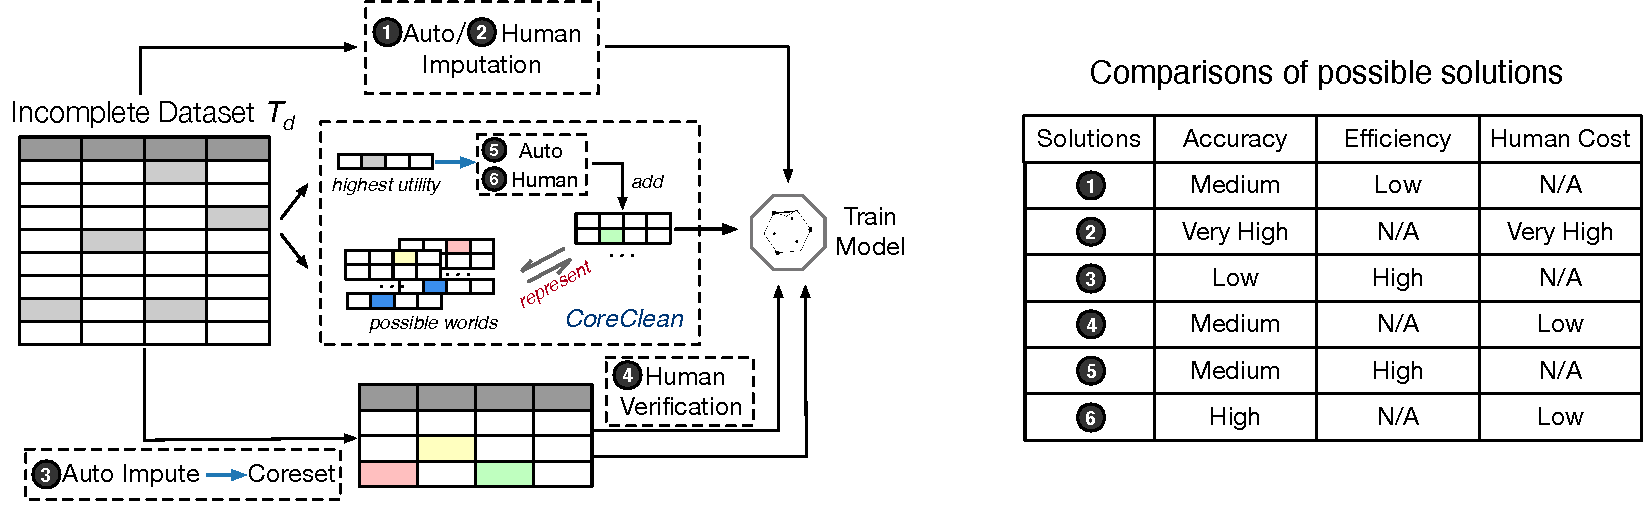
\includegraphics[width=1\textwidth]{figs/solutions}
%	\vspace{-3.2em}	
%	\caption{Possible solutions and \ours.}
	%\label{fig:coresets}
%\end{figure*}



%Hence, in this paper, we aim to solve the problem of \textit{how to select a good coreset that can achieve good performance when there exist incomplete tuples in the train dataset.}

%\add{Example~\ref{example:motexp} tells us that involving human into data cleaning can improve the accuracy. However, high human cost is unacceptable. Thus, introducing automatic data cleaning methods can significantly reduce the human cost.}

%\noindent \textbf{Key challenge.} As discussed, the above  intuitive solutions cannot achieve a good trade-off between data effectiveness and data efficiency. The essential challenge of  selecting a good coreset over incomplete data is that it is hard to know the ground truth of $D$, and thus the selected coreset is hard to represent the accurate complete version of $D$.

%To summarize, the key of coreset selection with incomplete data is to select a good coreset as a representative of the fully imputed train dataset. But unfortunately, $\trainc$ is rather hard to obtain  because of  two challenges. (1) There are many missing values (each  has several possible imputation choices) in $\train$, which constitute a large number  of possible worlds as candidates of $\trainc$. Hence, it is hard for an automatic method to accurately select one as $\trainc$ among these possible worlds . (2) Although we can hire  humans to accurately impute each value, it will introduce high cost. 

 

% \noindent \textbf{Our proposal.} 
% To address the challenge, we propose \ours that can select a well-performed coreset over incomplete data effectively and efficiently. 
% As discussed above, although we cannot get the ground truth in advance, \ours will select an informative coreset $C_C$ considering  the possible worlds of $D$. Overall, We formulate it as an optimization problem for selecting an expected optimal coreset that can represent the  possible worlds of $D$. We prove that this problem is NP-hard. We propose an approximate algorithm, with the main idea that greedily adds tuple with the highest utility  into the coreset. To be specific,  a tuple with a higher utility indicates that including the tuple can make the coreset better represent the possible worlds. Afterwards, $C_C$ can be imputed by automatic methods or human, and we can get $C_C^H$ and $C_C^A$ as shown in solution (3) and (4) respectively. To summarize, since $C_C$ is a good coreset, solution (3) can achieve a higher accuracy than solution (1), and solution (4) is competitive with solution (2) but with a much lower human cost.  
% %But the full data at hand $(\train)$ is incomplete, so  the utility is computed to measure whether the tuple can make the coreset well represent the possible worlds of $\train$.

% \noindent \textbf{Optimizations.} However, since the number of possible worlds of $D$ is extremely large because of there may exist many missing values in $D$, the computational cost of \ours is high. To address this,  we further propose imputation-in-the-loop strategies that  leverage automatic methods (solution (5)) or human (solution (6)) to impute the tuples in the coreset, once one or a small batch of incomplete tuples are added, which can greatly reduce the number of possible worlds. 	Please refer to Table~\ref{tab:compare} for the advantages and disadvantages of solutions (1)-(6). 


% \begin{table}[]
% 	\caption{Comparisons among possible solutions}\label{tab:compare}
% 	\begin{tabular}{|c|c|c|c|}
% 		\hline
% 		\multicolumn{1}{|l|}{Solution} & \multicolumn{1}{l|}{Accuracy} & \multicolumn{1}{l|}{Human Cost} & \multicolumn{1}{l|}{Machine Cost} \\ \hline
% 		(1)                            & Low                           & 0                               & Low                               \\ \hline
% 		(2)                            & High                          & High                            & Low                               \\ \hline
% 		(3)                            & Medium                        & 0                               & High                              \\ \hline
% 		(4)                            & High                          & Low                             & High                              \\ \hline
% 		(5)                            & Medium                        & 0                               & Low                               \\ \hline
% 		(6)                            & High                          & Low                             & Low                               \\ \hline
% 	\end{tabular}
% \end{table}

%There are many advantages. First, the number of possible worlds can be greatly reduced after some tuples are imputed,  and thereby the efficiency can be improved. Second, human is more accurate, so the human-in-the-loop strategy can help continuously improve the coreset quality. Third, since we just need to impute the incomplete tuples in the coreset, which is much smaller than $\train$, the cost is also greatly reduced.
 
 %\add{As shown in Figure~\ref{fig:mot_exp},  our Solution~\ding{204} can significantly reduce the human cost from 12500 to 153 without sacrificing the accuracy much \cc{(0.706)}.}


%\begin{figure}
%	\centering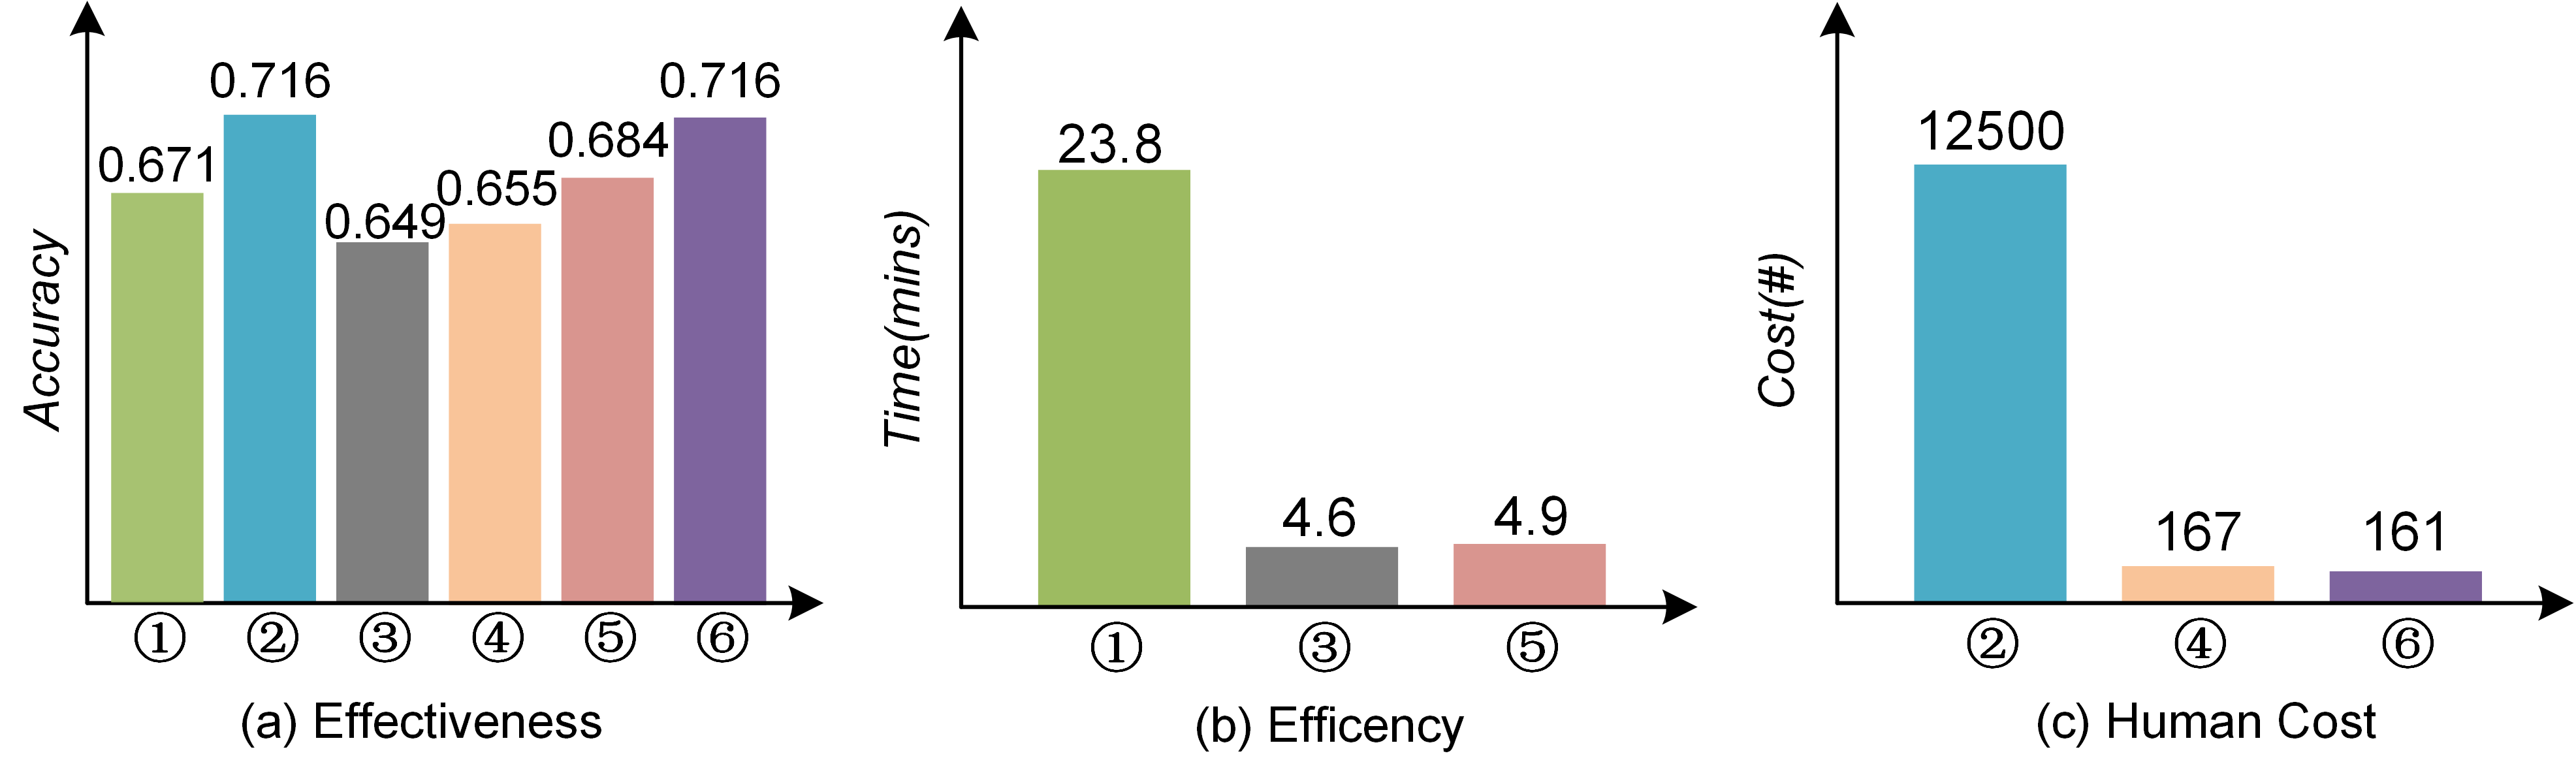
\includegraphics[width=\columnwidth]{figs/mot_exp.png}
%	\vspace{-1em}
%	\caption{Comparison with possible solutions and \ours.}
%	\label{fig:mot_exp}
%\end{figure}




 %and thus  tuples  are selected from the $\train$ iteratively and added into the coreset incrementally. To ensure the accuracy, we ask the humans to impute the selected tuples  iteratively such that  the  quality of the  selected tuples can be improved continuously in further iterations. Since we just leverage the human to impute the tuples within the selected coreset, the cost if greatly reduced (for \textbf{C2}).

% To summarize, we make the following contributions.

% \noindent (1) To the best of our knowledge, we are the first to study  coreset selection for supervised ML with incomplete data, and  formally define the problem (Section~\ref{sec:pre}). 

% \noindent (2) We prove the hardness of the problem. To solve the problem, we  propose a greedy algorithm with an approximate ratio using a single human iteration (Section~\ref{sec:without}). 

 
% \noindent (3) We further develop an imputation-in-the-loop strategy that   iteratively imputes one  or a small batch of tuple(s) during the coreset selection (Section~\ref{sec:human}).

% \noindent (4) We conduct extensive experiment on XX real-world datasets to show that \ours can select a well-performed coreset \cc{XX} while consuming a low human cost \cc{XX} (Section~\ref{sec:exp}).

% expected coreset- Np hard

% human in the loop

% In iterations, each iteration, incrementally select batch, ask human to impute, continuously improve the accuracy.


%automatically select a coreset $\core$ that is expected to be  optimal, and then impute the missing values among the small coreset by humans with a low cost, as shown in Figure~\ref{fig:coresets}-Solution \ding{204}.

%There are a multitude of reasons why they occur: ranging from human errors during data entry, incorrect sensor readings, to software bugs in data science pipelines [16]. Moreover, different from other types of errors (e.g., wrong names/addresses, unnormalized values, and violations of integrity constraints) that sometimes can be remained as they are, for ML modeling, these missing data fields must be deleted or imputed first.

%For many machine learning (ML) projects, the main bottleneck is the lack of high-quality train data, so as to produce high-quality ML model. However,  data collection or acquisition from various real-world datasets always incorporates errors in the train data such as missing values, outliers, inconsistency, etc, which may highly affect the model performance~\cite{}. Hence, it is indispensable to clean the data with the goal of improving the model.







%-- statistic-based, generative model-based, DL-based, but they are not accurate enough







%!TEX root = ../main.tex
\section{Background of Coreset Selection} 
\label{sec:pre}

In this section, we introduce the background of coreset selection on complete data, denoted by $\trainc$.
%, based on which we  illustrate the framework of  selecting the coreset over the incomplete data.

\subsection{Gradient Descent for Machine Learning}

{\bf Gradient descent}~\cite{lemarechal2012cauchy} is the most typical optimization algorithm to train ML models. 
At a high level, it  tweaks the parameters iteratively to minimize a given convex and differentiable function to its local minimum.

Let $\trainc = \{t_1, t_2, ..., t_n \}$ be a set of train tuples (without missing values), where $t_i = (\mathbf{x}_i, \mathbf{y}_i)$, $\mathbf{x}_i \in \mathbb{R}^d$ denotes the vector of features and $\mathbf{y}_i$ denotes the corresponding label. The goal of training on $\trainc$ is to find the best parameter  $\hypo^*$ of a model by minimizing the loss:

\vspace{-0.5em}
\begin{equation}\label{eqa:loss}
\hypo^* = \arg\min_{\hypo\in \vartheta}\fun(\hypo), \fun(\hypo)=\frac{1}{n}\sum_{i=1}^n\fun_i (\hypo, t_i) 
\end{equation}

\noindent where $\vartheta$ is the parameter space. For ease of representation, we abbreviate $\fun_i (\hypo, t_i)$ as $\fun_i(\hypo)$ to represent the loss of the $i$-th train example.  Generally speaking, the gradient descent approach is always applied to find the minimizer of  Eq.~\ref{eqa:loss}, where  the {\bf full gradient} (sum of the gradients over all training tuples), denoted by $\nabla\fun(\hypo) = \sum_{i=1}^{n}\nabla\fun_i(\hypo)$, has to be computed iteratively. 

Besides incremental gradient methods like stochastic gradient descent (SGD) that can be leveraged to accelerate the iterative gradient computation, there are other popular and orthogonal methods, such as coreset, which will be discussed next.

%it is still expensive when there are a large number of train tuples.


\subsection{Coreset over Complete Data}
\label{subset:sigletable}

\stitle{Coreset.} To make training more efficient, instead of learning from entire $\trainc$, one research question  is that whether we can compute a small subset $\corefunc(\trainc)$ of $\trainc$ such that learning with $\corefunc(\trainc)$ can hopefully achieve the same performance as learning with $\trainc$.
%
This small selected subset is called {\bf coreset}~\cite{DBLP:journals/corr/abs-2011-09384,munteanu2018coresets}.
%
In the following, we simply write $\corefunc(\trainc)$ as $\core$ when it is clear from the context.

The state-of-the-art coreset selection solutions are mostly based on gradient approximation~\cite{DBLP:conf/aaai/KillamsettySRI21, DBLP:conf/icml/MirzasoleimanBL20}.
Suppose that $\theta$ denotes the parameter of an ML model trained over the full dataset, and $\theta'$ denotes the parameter of the same model trained over  the coreset.   Intuitively,   the objective of gradient approximation for coreset selection is to make $\nabla\fun(\hypo')$ as close as possible to $\nabla\fun(\hypo)$. To this end, existing solutions focus on \textit{selecting the coreset that  minimizes the upper bound of gradient approximation error} ($\lVert  \nabla\fun(\hypo) - \nabla\fun(\hypo')  \rVert$). Next, let's formally define it from scratch.
%


%Based on gradient approximation, existing solutions can lead to good performance with theoretical guarantees, \ie $\nabla\fun(\hypo)$ is upper-bounded by $\nabla\fun(\hypo')$. Next let's formally define it.

%Given a large training dataset $\train$, in general,  coreset selection in ML aims to compute a small subset $\core$ of $\train$ such that training on  $\core$ can hopefully has the same performance as training on $\train$, which is inefficient due to the large amount of data.  Although there exist a line of approaches, coreset selection considering the gradient approximation is a commonly-used one because of the good performance with theoretical guarantees. 


%\subsection{Problem definition}  \label{subsec:def}

%In this section, we first introduce the  definition of coreset in the field of ML, and then formally define our problem of coreset selection over multiple tables.

%\subsubsection{Coreset selection over a single table}\label{subsubsec:singleTab}  Given a large training dataset $\train$, in general,  coreset selection in ML aims to compute a small subset $\core$ of $\train$ such that training on  $\core$ can hopefully has the same performance as training on $\train$, which is inefficient due to the large amount of data.  Although there exist a line of approaches, coreset selection considering the gradient approximation is a commonly-used one because of the good performance with theoretical guarantees. 

% \noindent \textbf{Training on $\train$.}  Formally speaking, $\train = \{t_1, t_2, ..., t_n \}$ is a set of labeled training tuples, where $t_i = (\mathbf{x}_i, \mathbf{y}_i)$, $\mathbf{x}_i \in \mathbb{R}^d$ denotes the feature vector and $\mathbf{y}_i$ is the corresponding labels.
% The objective of training on $\train$ is to compute the best parameter  $\hypo^*$ to minimize the loss


% \begin{equation}\label{eqa:loss}
%     \fun(\hypo)=\frac{1}{n}\sum_{i=1}^n\fun_i (\hypo, t_i), \hypo^* = \arg\min_{\hypo\in \vartheta}\fun(\hypo)
% \end{equation}

% \noindent where $\vartheta$ denotes the parameter space and for ease of representation, we just use $\fun_i(\hypo)$ to denote the loss of the $i$-th training example, \ie $\fun_i (\hypo, t_i)$.  Typically, the gradient descent method is always applied to optimize Eq.~\ref{eqa:loss}, where  the full gradient, \ie $\nabla\fun(\hypo)$ is required to compute iteratively. Although some classic incremental gradient methods such as  stochastic gradient descent (SGD), can be utilized to accelerate this process, it is still expensive when there are massive training tuples.



\stitle{Gradient-based coreset selection} %To alleviate the above issue, coreset is proposed to  
%It is to select a subset $\core\subseteq \train$ such that the sum of weighted gradients of tuples in $\core$ can well approximate the full gradient $\sum_{i=1}^{n}\nabla\fun_i(\hypo)$. The goal is, training on $\core$ based on the estimated gradient is very likely to achieve the same performance as training on the entire training set. Formally, it is defined as follows:
%Let $\nabla\fun(\hypo) = \sum_{i=1}^{n}\nabla\fun_i(\hypo)$ be the full gradient training using the entire train dataset, the problem of coreset selection 
is to minimize the {\bf gradient approximation error (GA error)} between the full gradient \wrt $\trainc$ and the weighted sum of gradients \wrt the coreset $C$ (or coreset gradient).
Formally, Eq.~\ref{eqa:coreset} tries to minimize the  GA error 
by considering all possible parameters $\hypo\in\vartheta$ (\ie $\max\limits_{\hypo\in\vartheta}$), where ``$\| \cdot \|$'' denotes the normed difference. Next, we introduce the coreset gradient.
%in details.

\vspace{-1em}
\begin{equation}\label{eqa:coreset}
\begin{array}{l}
\core^* = \argmin\limits_{C\subseteq \trainc, w_j \geq 0}
\max\limits_{\hypo\in\vartheta}
\lVert 
\underbrace{
	\underbrace{\sum\limits_{i=1}^n\df_i(\hypo)}_{\text{full gradient}} - 
	\underbrace{\sum\limits_{j=1}^{|C|}w_j\df_{\gamma(j)}(\hypo)}_{\text{coreset gradient}} 
}_{\textbf{gradient approximation error}}
\rVert, 
\\ 
s.t.~|C| \le \numcore %\le \epsilon
\end{array}
\end{equation}




%The {\bf full gradient} has been defined earlier as $\nabla\fun(\hypo) = \sum_{i=1}^{n}\nabla\fun_i(\hypo)$.Next, let's focus on explaining how to compute the {\bf coreset gradient} in Eq.~\ref{eqa:coreset}.
%
%\noindent since  $\core\subseteq \train$ with the size no more than $K$,
Because the coreset is a subset of the complete dataset (\ie $C \subseteq \trainc$),
we use $\gamma(j) = i$ (where $j\in[1,|C|], i\in[1,n]$) to denote that the $j$-th tuple in $\core$ (denoted by $c_j$) is the $i$-th tuple in $\trainc$, \ie $t_i$. In other words, $\gamma$ is an index mapping from $\core$ to $\trainc$. 

Recall that the key idea of the coreset is to \textit{use a subset of tuples to represent the entire set}.  Eq.~\ref{eqa:coreset} potentially contains another important mapping $\phi$ from $\trainc$ to $\core$ to indicate this, \ie $\phi(i) = j, i\in[1,n],  j\in[1,|C|]$, which is highly related to the weight. Specifically, let $\phi(i) = j$ denote that we will assign  $t_i$ to $c_j$ (use $c_j$ to represent $t_i$) and use $\df_{\gamma(j)}$  to represent $\df_i$. Each $t_i$ will be assigned to one and only one $c_j$, but each  $c_j$ might be assigned with multiple tuples in $\trainc$. Based on $\phi$,
$w_j$ is defined as the weight of  the $c_j$, which is the number of tuples in $\trainc$ assigned to the $c_j$, \ie $w_j = |\{t_i|\phi(i) = j, i\in[1,n]\}|$ ($c_j$ is utilized to represent $w_j$ tuples in $\trainc$). 

Next let's use an example to better illustrate Eq.~\ref{eqa:coreset}.



\begin{example}\label{example:singletable}
	Let's consider a  case of the gradients of each tuple, as shown in Figure~\ref{fig:overviewSingle}. Suppose that for any $\hypo$, $\df_1(\hypo)\approx\df_2(\hypo)$, $\df_3(\hypo)\approx\df_4(\hypo)\approx\df_5(\hypo)\approx\df_6(\hypo)$ and $\df_7(\hypo)\approx\df_8(\hypo)$. In this case, based on Eq.~\ref{eqa:coreset}, if one wants to find an optimal coreset with a size of  3, \ie $\numcore=3$, the solution can be $C^* = \{t_2, t_5, t_7\}$ ($\gamma(1)=2, \gamma(2)=5$ and $\gamma(3)=7$), associated with $w_1=2, w_2=4, w_3=2$ because $\phi(1) = \phi(2) = 1, \phi(3) = \phi(4) = \phi(5) = \phi(6) = 2 $ and $\phi(7) = \phi(8) = 3$. In this way, $C^*$ can be one of the optimal coresets that can well approximate the full gradient because  $\lVert \sum\limits_{i=1}^8\df_i(\hypo) - \sum\limits_{j=1}^{3}w_j\df_{\gamma(j)}(\hypo) \rVert  $ is minimized, which is close to 0.
\end{example}


\begin{figure}[t]
	\centering
	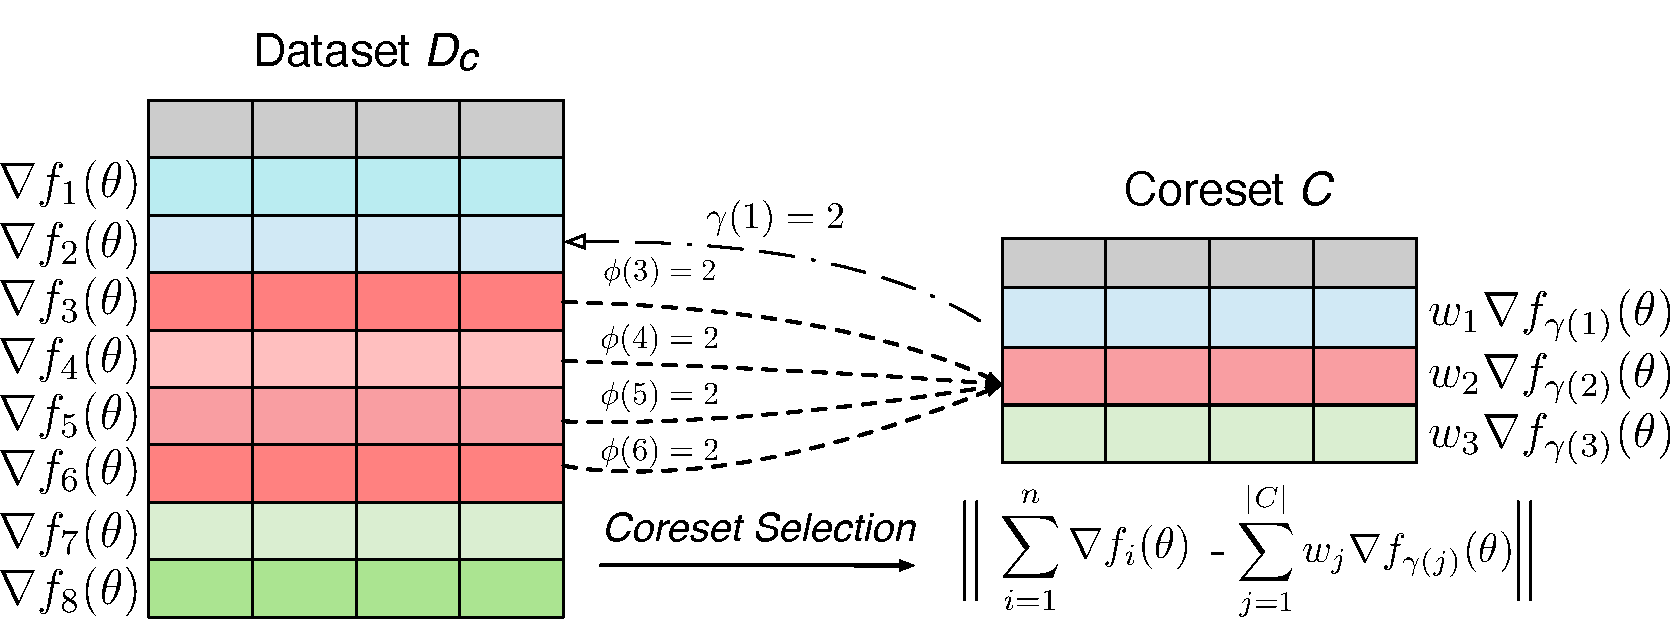
\includegraphics[width=0.6\textwidth]{figs/coresetExample}
%	\vspace{-2em}
	\caption{Example of coreset selection.}
	\label{fig:overviewSingle}
%	\vspace{-2em}
\end{figure}

\stitle{Key observation.} We can observe from Example~\ref{example:singletable} that in order to minimize the GA error, we should set $\phi(i) = j$, where $\df_i$ and $\df_{\gamma(j)}$ are likely to be close. 
Therefore, computing the coreset is similar to computing the $\numcore$ exemplars~\cite{rdusseeun1987clustering} of the gradients, if all the gradients of tuples can be computed.


\stitle{Upper bound minimization of GA error.} We can see from Eq.~\ref{eqa:coreset} that to solve the equation, the gradients have to be computed, which have a close relationship with the parameter  $\theta$. However, the main bottleneck is that  the entire parameter space $\vartheta$ is too expensive to explore. Hence, a typical solution is to  first compute the upper bound of  GA error (Eq.~\ref{eqa:triangle}),  then generalize~\cite{hofmann2015variance, allen2016exploiting,DBLP:conf/icml/MirzasoleimanBL20} the upper bound computation to the entire parameter space (Eq.~\ref{equation:convex}), and finally select the coreset to minimize the bound. To be specific, using the triangle equation, for any particular $\theta$, we have:

\vspace{-0.5em}
\begin{equation}\label{eqa:triangle}\small
\begin{array}{l}
\lVert 
\sum\limits_{i=1}^n\df_i(\hypo) - 
\sum\limits_{j=1}^{|C|}w_j\df_{\gamma(j)}(\hypo) 
\rVert \leq \sum\limits_{i=1}^n \lVert \df_i(\hypo) - \df_{\gamma(\phi_\theta(i))}(\hypo) \rVert
\end{array}
\end{equation}

Together with the aforementioned observation, given a coreset $\core$, the upper bound is minimized when  $\phi$ assigns
every tuple $t_i$ to the tuple in $\core$ with most gradient similarity, \ie $\lVert 
\sum\limits_{i=1}^n\df_i(\hypo) - 
\sum\limits_{j=1}^{|C|}w_j\df_{\gamma(j)}(\hypo) 
\rVert \leq \sum\limits_{i=1}^n \min \limits_{c_j\in\core}\lVert \df_i(\hypo) - \df_{\gamma(j)}(\hypo) \rVert$.

\stitle{For the entire space $\vartheta$},  it has been proved in recent works~\cite{hofmann2015variance, allen2016exploiting,DBLP:conf/icml/MirzasoleimanBL20} that for convex ML problems (corresponding to an optimization problem in which the objective function is a convex function), the normed gradient difference between tuples can be efficiently bounded by:

\vspace{-0.5em}
\begin{equation}\label{equation:convex}
\begin{aligned}
\forall  i, j, \max\limits_{\hypo\in\vartheta}\lVert \df_i(\hypo) - \df_j(\hypo) \rVert \le \max\limits_{\hypo\in\vartheta}\mathcal{O}(\lVert \theta \rVert) \cdot \lVert \mathbf{x}_i - \mathbf{x}_j \rVert
\end{aligned}
\end{equation}

\noindent where $\lVert \mathbf{x}_i - \mathbf{x}_j \rVert$ is the Euclidean distance between  feature vectors of two tuples, namely \textit{feature distance}, and 
 $\mathcal{O}(\lVert \theta \rVert)$ is a constant. Hence, we can conclude that \textbf{GA error can be bounded independent of the optimization problem in practice, \ie any particular $\theta$}. Finally, considering Eq.~\ref{eqa:triangle} and  Eq.~\ref{equation:convex} together,  \textit{the coreset selection problem can be converted to:}
 
 \vspace{-0.5em}
 \begin{equation}\label{eqa:coreset2}
 \core^* = \argmin\limits_{C\subseteq \trainc}\sum_{i=1}^n \min_{c_j\in C}\dist_{ij}, \text{ s.t. } |C| \le \numcore %\le \epsilon
 \end{equation}
 
 \noindent where $\dist_{ij} = \lVert
 \mathbf{x}_i - \mathbf{x}_{\gamma(j)}  \rVert$ for ease of representation. The above equation indicates that given a train data $\trainc$ and a coreset $\core$, we use  $S = \sum_{i=1}^n \min_{c_j\in C}\dist_{ij}$ to score the coreset. The lower the score, the smaller upper bound of the GA error we can get, which indicates a better coreset.
 To summarize, solving Eq.~\ref{eqa:coreset2} is to minimize the upper bound of the GA error (\ie select the coreset with the lowest score) by just considering the feature vectors of the training tuples without  training in advance.
 
Note that Eq.~\ref{equation:convex} holds for tuples associated with the same label~\cite{allen2016exploiting, hofmann2015variance}. Therefore, in practice, we respectively select coresets for tuples with different labels and combine them. Suppose that we aim to select a coreset with size  $K$ for a binary classification task (label 1: 60\%, label 0: 40\%), so we select a coreset with size 60\%$K$ for tuples with label 1 and another one with 40\%$K$ for tuples with label 0.
%we need to select subsets of coresets for tuples with dierent labels
%and combine them. For example, given a binary classication task
%(30\% of label 0 and 70\% with label 1), to select a coreset with size $K$,
%we separately select a coreset of size 30\%$K$ for tuples with label 0
%and another coreset of size 70\%$K$ for tuples with label 1, and then
%merge them. For regression tasks, we will cluster tuples with similar labels, select subsets of coresets for these clusters and merge them.
 
\stitle{Our scope.} In this paper, we focus on the convex problems (\eg logistic regression, support vector machine, etc.) because for such
problems the gradient difference can be well bounded by the difference
between feature vectors. 
%
Note that, for other ML algorithms such as deep neural networks, they can also be trained using selected coreset to achieve good training accuracy (see Section~\ref{sec:exp} for our experimental findings).

% \cc{For other ML algorithms, like
% deep learning, can also train on the selected the coreset. As shown in Section~\ref{sec:exp}, good performance can also be achieved although it is hard to have a theoretical gradient bound.}

%%!TEX root = ../main.tex
%\vspace{-1em}
\section{Related Work}\label{sec:related}

\noindent{\bf Task-agnostic incomplete data imputation.}
Data imputation has been widely studied for  years. Existing  methods can be divided into two categories: statistic-based methods and learning-based methods. The former one always uses the statistic information~\cite{DBLP:journals/tsmc/FarhangfarKP07, DBLP:conf/sigmod/MayfieldNP10} (like mean, median or mode) to impute the missing values. Also, some methods compute the similarity of the incomplete tuples to the complete tuples and use the most similar one to impute the missing values~\cite{altman1992introduction, DBLP:journals/artmed/JerezMGARMF10, DBLP:conf/isese/TwalaCS05}. Recently, to improve the imputation accuracy,   many learning-based methods focus on how to use ML to learn the data distribution (\eg MissForest imputation~\cite{DBLP:journals/bioinformatics/StekhovenB12}, MICE~\cite{royston2011multiple},  IIM~\cite{DBLP:conf/icde/ZhangSSW19}), and then  use the trained model to predict the missing values. Besides traditional ML models, some deep learning models are also used for data imputation (\eg  autoencoder~\cite{DBLP:journals/corr/GondaraW17, mccoy2018variational, DBLP:journals/pr/NazabalOGV20}, GANs~\cite{DBLP:journals/nn/SpinelliSU20, DBLP:conf/icml/YoonJS18}).
 
\noindent{\bf Coreset selection.} A previous work~\cite{} has studied how to select a well-performed coreset over incomplete tuples. The extension to the previous study in this work is four-fold. First, we propose a new framework that incorporates the group-based strategy into the coreset selection process with incomplete data. Secondly, we theoretically analyze that the group-based strategy can still have a bounded GA error. Third, we propose an efficient solution to estimate the upper bound, and several strategies to reduce the number of possible worlds. Fourth, two large datasets are added and multiple experiments are conducted to demonstrate the efficacy of our proposed methods. 

%
Besides, Huang et al.~\cite{DBLP:conf/icml/HuangHLFD21} studied how to compute and continuously update the coreset while training. %, which aims  to utilize the loss of training tuples  to approximate the overall training loss of the entire training set. 
But it is rather time-consuming because of the training process. 
 To solve this problem, works~\cite{DBLP:conf/icml/CampbellB18, DBLP:journals/corr/BravermanFL16}   selected the coreset without training in advance, but they can only be customized to particular model types respectively. %The basic idea is to compute a sensitive score for each tuple, and the higher the score, the more likely the tuple should be in the coreset. 
 Another line of works~\cite{DBLP:conf/icml/MirzasoleimanBL20, DBLP:conf/nips/MirzasoleimanCL20, DBLP:conf/emnlp/KirchhoffB14} focused on selecting the coreset to approximate the full gradient without training in advance for multiple model types, which is regarded as an optimization problem that can be solved  by the three nested loops framework (see Section~\ref{subset:sigletable}).

In short, none of them considers coreset selection over incomplete data. Different from them, we make the first attempt to select coresets over incomplete data.

\noindent{\bf Data cleaning for ML.} Recently, there have  been several works that clean the data to optimize the ML model. 
In contrast to the above discussion about task-agnostic incomplete data imputation, data cleaning for ML is task-aware, which triggers new technical challenges.
SampleClean~\cite{DBLP:journals/debu/KrishnanWFGKM015} focuses on cleaning selected samples, so as to answer  SQL aggregate  queries  more efficiently, but it is not for any model.
%
 CPClean~\cite{DBLP:journals/pvldb/KarlasLWGC0020} proposes certain prediction to impute missing data for optimizing ML models. Different from us, it is customized to nearest neighbor classifiers rather than convex models solved by the gradient decent algorithm. 
  %
  BoostClean~\cite{DBLP:journals/corr/abs-1711-01299} regards data cleaning as a boosting problem that iteratively
 selects from a predefined set of cleaning algorithms, so as to continuously maximize the accuracy of  a validation set with training iteratively. 
Closer to our work is ActiveClean~\cite{DBLP:journals/pvldb/KrishnanWWFG16}, which progressively cleans the data tuples that are likely to much influence the model   measured by the gradients. 
%\cc{
Different from us,  given a budget $K$, we can select the coreset without training, but ActiveClean needs to train iteratively  and label a set of   validation  dataset.  We empirically show that our method outperforms ActiveClean on model accuracy and efficiency in Section~\ref{sec:exp}.
%}.
%(2) ActiveClean uses heuristics to measure the influence of tuples to the model gradients, which may not be accurate.
% Moreover, we  ActiveClean to the data imputation problem and compare with it in Section~\ref{sec:exp}.}

%ActiveClean iteratively estimates the impact of the dirty data and samples a batch of dirty data that have the most impact on the model. Then, ActiveClean asks human to clean the batch of dirty data. The main difference between ActiveClean and \ours is ActiveClean needs to iteratively train the model, since it relies on the feedback from both human and model to estimate the impact of the dirty data.


\noindent{\bf Data Preparation for AI.}
Data preparation~\cite{chai2020crowdchart} can be utilized to improve the effectiveness of ML model, including data discovery~\cite{liu2021automatic, chai2022selective, liu2022feature},  data cleaning~\cite{hao2020outdated,chai2020human}, data labeling~\cite{chai2016cost, chai2018partial, li2018cdb}, data cleaning~\cite{miao2022experimental, gao2018query,miao2018incomplete, miao2021efficient,wu2022interactive,ge2020hybrid} and data exploration~\cite{qin2020interactively,qin2021ranking}.

\section{Coreset Over Incomplete Data} % ($\train$)}
\label{sec:overview}

In this section, we will formally define the problem of coreset selection over incomplete data (Section~\ref{subsec:problem}) and then describe our proposed framework to solve the problem  (Section~\ref{subsec:framework}).

\subsection{Problem Definition}
\label{subsec:problem}



As discussed above, we have to compute the coreset score $S$, so as to produce a good coreset.  To this end, the feature distances can be computed as a pre-processing step, based on which the coreset score can be computed. However, when there exists incomplete data with missing values, even the feature distances are hard to compute accurately, let alone selecting a proper coreset.

\stitle{Incomplete data.}
Formally, suppose that $\train$ has $M$ attributes, denoted by $\{\attr_1, \attr_2, ..., \attr_M\}$. Each attribute $\attr_m, m\in [1,M]$ represents a  domain set including the \texttt{Null}, (\ie $\texttt{Null} \in \attr_m$), in which each tuple in $\train$ can take value on this attribute. $|\attr_m|$ denotes the domain size. Then, each tuple $t_i \in \attr_1 \times \attr_2 \times, ..., \times \attr_m$. Let $t_i[m]$ denote the value of the $m-$th attribute of $t_i$, \ie $t_i[m] \in \attr_m$.
 
 
 For a tuple $t_i\in \train$, if $\exists~ t_i[m] = \texttt{Null},m\in [1,M] $, $t_i$ is an incomplete tuple, denoted by $\mathbb{I}[t_i] = 1$, otherwise $\mathbb{I}[t_i] = 0$.
Let us better illustrate this using an example. 

\begin{example} \label{example:incomplete}
	As shown in  Figure~\ref{fig:missing}(a), there are 6 tuples in the table $\train$ with five attributes (an excerpt from a large table). For example, $\attr_2$ is the \texttt{Gender} attribute, \ie $\attr_2 = \{ \texttt{M}, \texttt{F}, \texttt{Null} \}$.
	 Among these tuples, $t_2, t_3, t_4, t_6$ have missing values, \eg $\mathbb{I}[t_2] = 1, \mathbb{I}[t_1] = 0$. Given a coreset as shown on the right side, if there are no missing values, we can assign each tuple $t_i\in \train$ to its most similar tuple in $\core$ (compute $\min_{c_j\in C}\dist_{ij}$), and then sum these feature distances up to  compute the coreset score  $S$. However, given these missing values, the feature distances cannot be computed accurately (\eg $s_{12}, s_{13}, s_{22}$, etc.), and thus the assignment of tuples in $\train$ cannot be determined precisely. Hence, the coreset score is not precise, and thereby leads to a  coreset that cannot well represent the full complete (clean) data. 
	 \vspace{-0.3em}
\end{example}


\begin{figure}[t]
	\centering
	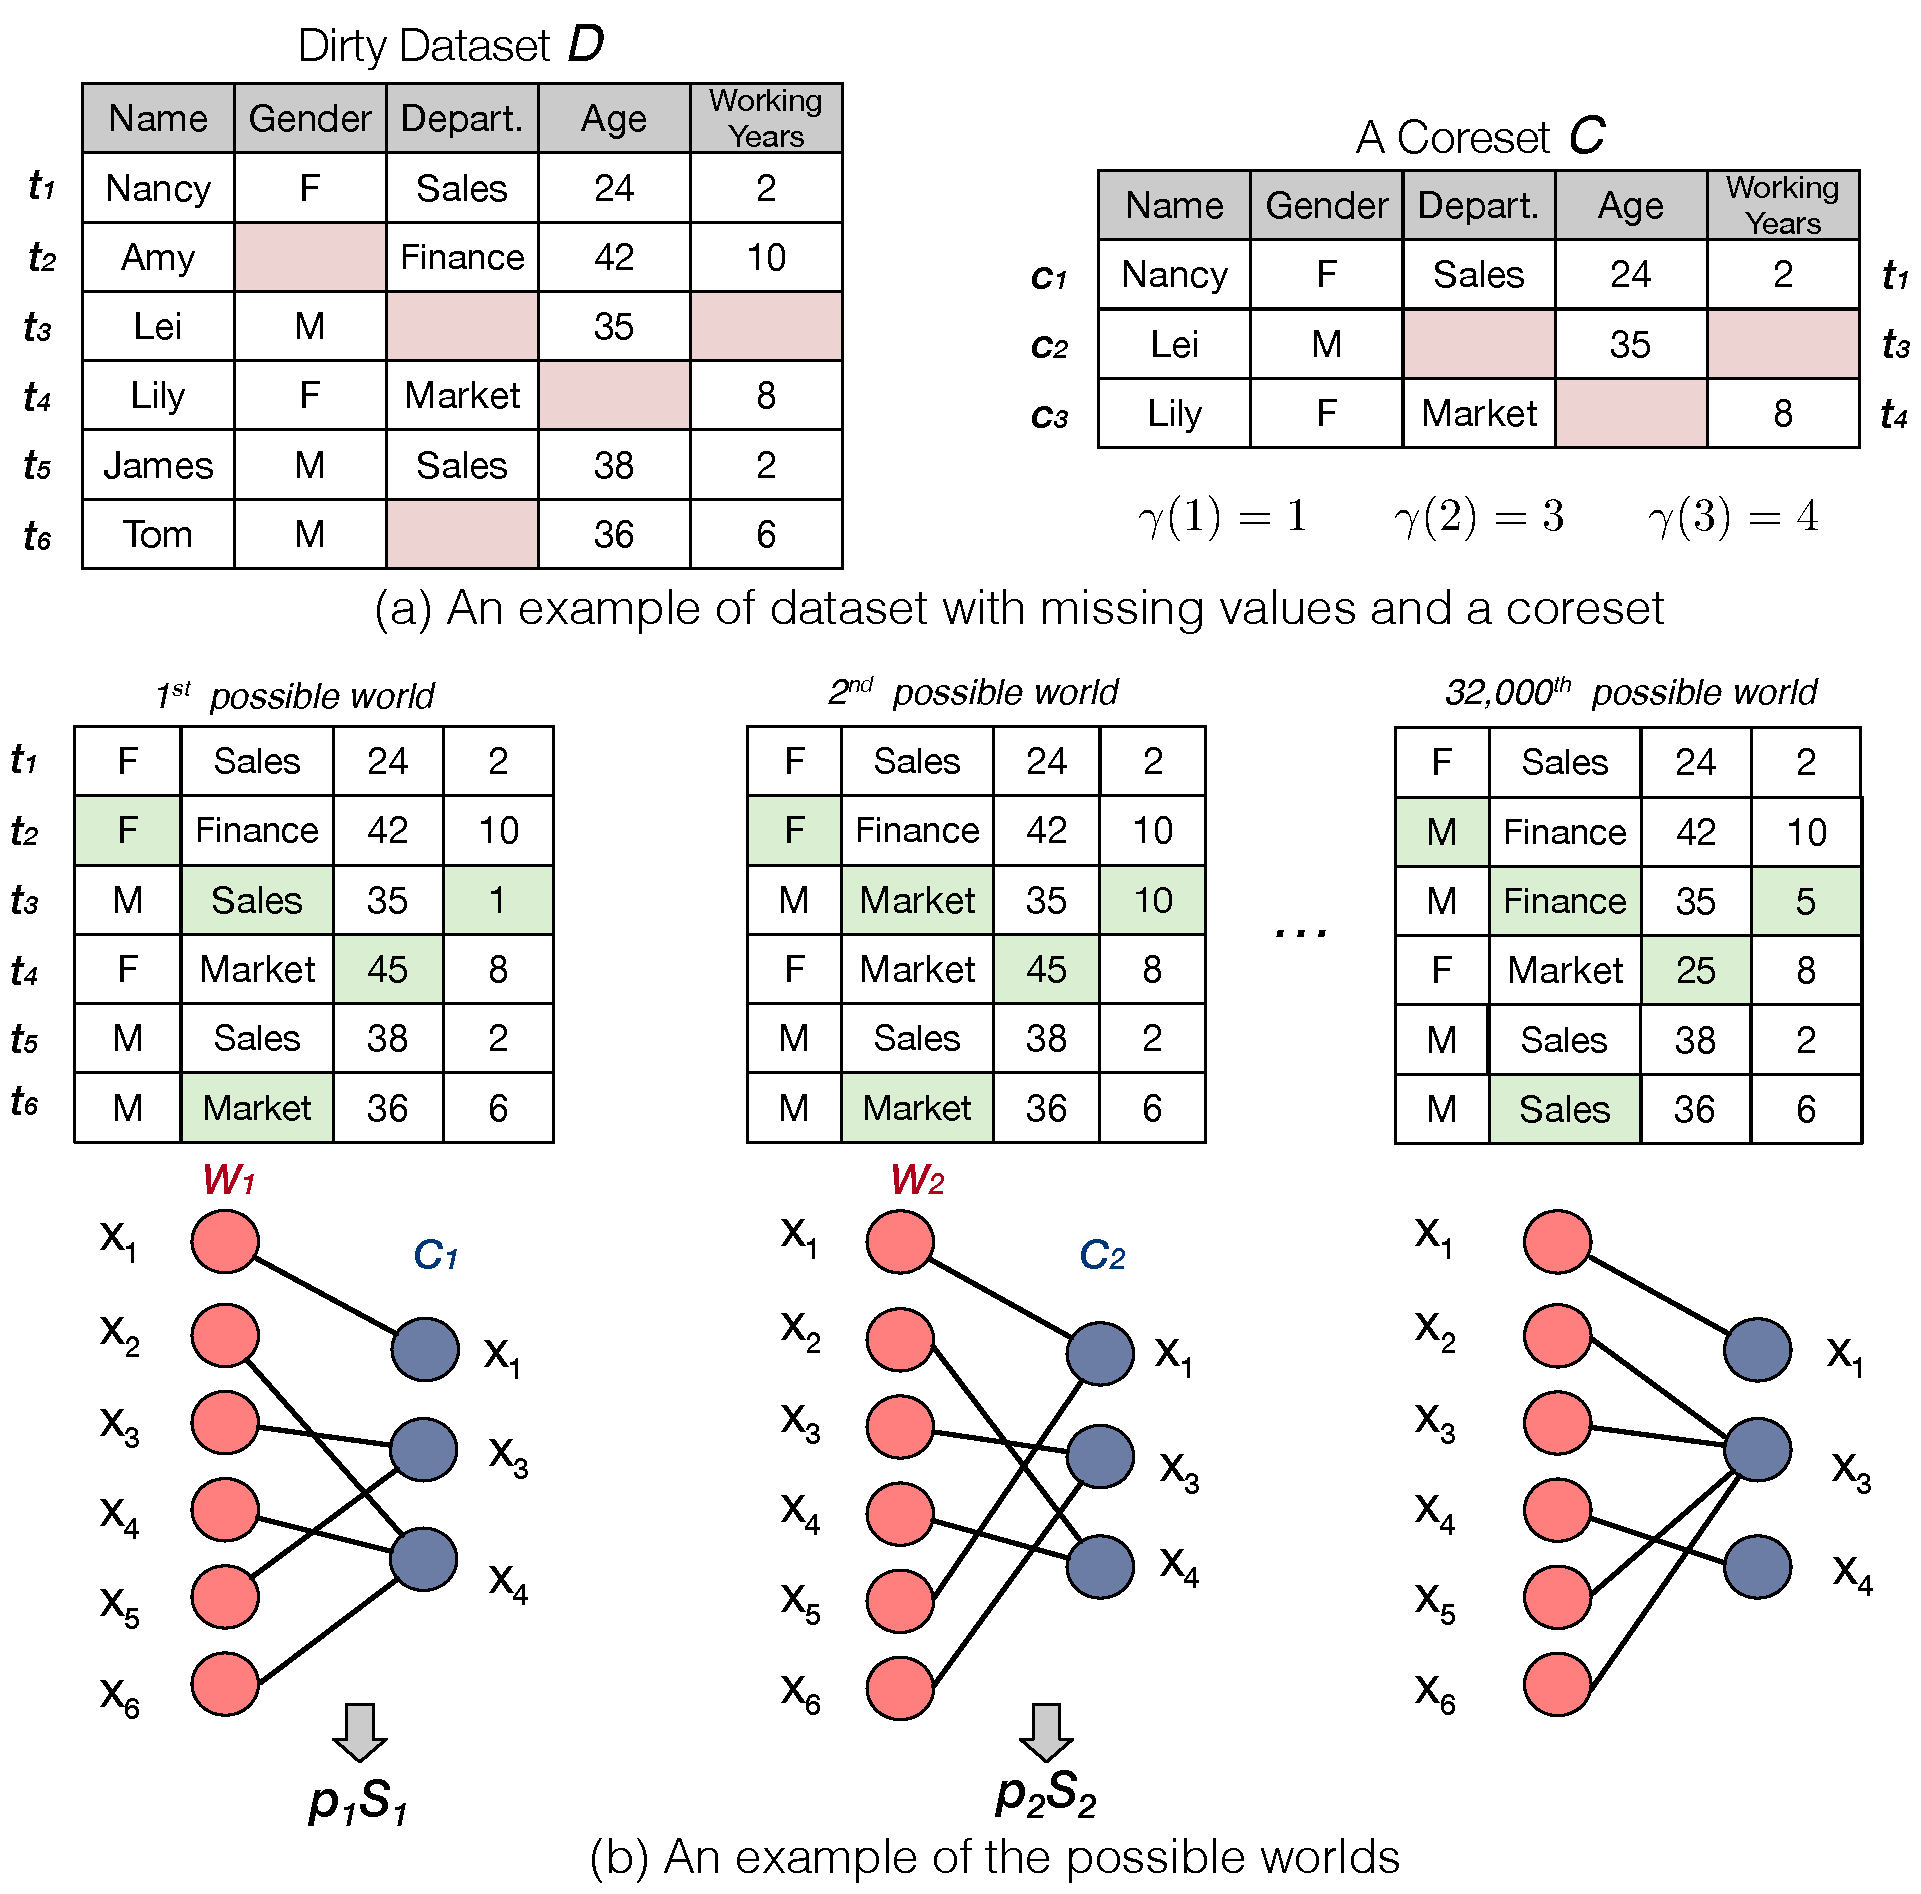
\includegraphics[width=0.6\textwidth]{figs/missExample}
%	\vspace{-2.5em}
	\caption{Example of coreset selection with missing values}.
	\label{fig:missing}
%	\vspace{-1.7em}
\end{figure}

As discussed above, \textit{imputation before coreset selection} suffers from either large cost (human imputation) or large number of possible repairs (automatic imputation), while \textit{imputation after coreset selection} cannot obtain a good coreset  because of the inaccurate feature distance computation (see Example~\ref{example:incomplete}).

%\etitle{Imputation before Coreset Selection.}
%One natural direction is to impute missing values before coreset selection. 
%As discussed in Section~\ref{sec:intro}, we can ask humans to impute the missing values first accurately and then select the coreset, but it is rather expensive given a large number of missing values, as discussed in Case (1) in Section~\ref{sec:intro}. 
%
%Alternatively, we can choose existing automatic imputation methods, as shown in Case (2).
%However, automatic  methods typically cannot ensure high imputation accuracy because these missing values result in a large number of possible repairs, which constitute a large search space. Therefore, it is hard for  automatic methods to identify an accurate imputation, based on which the selected coreset is also not good enough.
%the  they are not always accurate because these missing values result in a large number of possible worlds, and then produce a very large search space. 

%\etitle{Imputation after Coreset Selection.} Instead, we can select the coreset first, and then leverage human or automatic methods to impute the coreset, as illustrated in Case (3) and (4). However, the coreset directly selected from  incomplete data $\train$ is not good enough because of the inaccurate feature distance computation (see Example~\ref{example:incomplete}), and thus although humans can provide accurate imputation with a low cost, it is also hard for the coreset to well represent  $\trainc$.

Therefore, an essential problem is to select a good coreset that can represent the complete dataset $\trainc$, which relies on accurate coreset score computation given $\trainc$ that is the unknown ground truth.
%
Fortunately, the possible repairs of $\train$ can be modeled by possible worlds~\cite{DBLP:journals/tods/DengFG16, DBLP:conf/pods/ArenasBC99, DBLP:series/synthesis/2011Bertossi, DBLP:conf/pods/Bertossi19}, based on which we can effectively select the coreset over incomplete data.

%\cc{In short, the key is to select a good coreset that can represent $\trainc$, which relies on accurate coreset score computation given $\trainc$ and a coreset, but unfortunately $\trainc$ is the ground truth unknown in advance, 
%	To alleviate this issue, we can model possible repairs of $\train$ such that the selected coreset can represent the expected situation of $\trainc$.
%To this end, we leverage the  possible worlds that are widely-used in data repairing~\cite{DBLP:journals/tods/DengFG16, DBLP:conf/pods/ArenasBC99, DBLP:series/synthesis/2011Bertossi, DBLP:conf/pods/Bertossi19} to select the coreset over incomplete data.}


%Next, we first formally define the possible worlds.

%\begin{definition}(Possible worlds) 
\stitle{Possible worlds.}
 Given   the incomplete dataset $\train$, $\forall t \in \train$ and $\mathbb{I}[t] = 1$, $ \forall t[m] = \texttt{Null}, m \in[1, M]$, we assign a value in $\attr_m\setminus \{ \texttt{Null}\}$ to $t[m]$ as an imputation (\aka a possible repair). Thus, we have an assignment for all the missing values in $\train$, which corresponds to a possible world $\world$. Since there exist a large number of possible assignments,
 we define the set of possible worlds as $\worlds=\{\world_k| k\in [1,|\worlds|] \}$.
 %\end{definition}
 
 Let us better illustrate this using an example.
	

\begin{example}
	
Given $\train$, for tuples $t_2, t_3, t_4, t_6$ with missing values, we have a large number of possible assignment  as shown in Figure.~\ref{fig:missing}(b), each of which corresponds to a possible world (we omit the \texttt{Name} attribute because there is no missing value on this attribute). Suppose that there are 2 (4/100/10) types of values of the attribute \texttt{Gender} (\texttt{Department}/\texttt{Age}/\texttt{Working years}), there exist 32,000 possible worlds in total. %\cc{
	%}
\vspace{-0.3em}
\end{example}

Note that for numerical attributes, we will bin them into different buckets, such that we can treat them as categorical values and avoid the unlimited number of possible worlds.

Even with  possible worlds, the score computation of coreset remains challenging. 
Each possible world of $\train$ is a complete dataset, and thus given a coreset, the score can be directly computed considering the feature distances, as discussed in Section~\ref{subset:sigletable}. However, the crucial issue is that each possible world could be the ground truth, \ie $\trainc$, but each one leads to a different score.
%
%\nan{Only saying ``the score can be much different'' is not strong enough for the challenge. We need to use more conceptual idea here. \textbf{Why hard when using possible words?}}

\begin{example}
\label{exam:diffscores}
	As shown in Figure.~\ref{fig:missing}(b), the two possible worlds $\world_1$ and $\world_2$ are only different in $t_3$, leading to a different feature vector $\mathbf{x}_3$, which makes the score computation a difference. To be specific, given the same coreset $\core$ with tuples $t_1 (c_1)$, $t_3 (c_2)$ and $t_4 (c_3)$, because of a different $\mathbf{x}_3$, the closest feature distance of $\mathbf{x}_5$ in $\world_2$ becomes $\mathbf{x}_1$, rather than $\mathbf{x}_3$ in $\world_1$. And the closest feature distance of $\mathbf{x}_6$ in $\world_2$ becomes $\mathbf{x}_3$, rather than $\mathbf{x}_4$ in $\world_1$. Therefore, the coreset scores, %($S=\sum_{i=1}^n \min_{c_j\in C}\dist_{ij}$), 
	\ie the sum of these closest feature distances of tuples are different among possible worlds.
	\vspace{-0.3em}
\end{example}

Example~\ref{exam:diffscores} shows that different possible worlds make the mapping $\phi$ different, which leads to different scores. Hence, to get a good coreset without the ground truth, an intuitive solution is to compute the expected coreset score considering all possible worlds. By doing so, although we cannot get the complete data ($\trainc$) in advance, we can focus on how to select an informative coreset that can represent the possible worlds of $\train$.

Next, we formally define the studied problem.

%\begin{definition}[Expected optimal coreset selection over incomplete data]
\stitle{Expected optimal coreset selection over incomplete data.}
	 %Given $\train$ and $\core$, we have possible worlds $\{W_k\}$ as well as the corresponding coresets $\{C_k\}$. 
	 Given $\train$, we have a number of possible worlds $\worlds=\{W_k\}$. Then given a subset (coreset) $C\subset \train$,  
	  for different $W_k$, we have the corresponding $C_k$ with the same tuples as $C$ but probably different imputations.
	   For $C_k$, we can compute a score $S_k = \sum_{i=1}^n \min_{c_j\in C_k}\dist_{ij}$, where $\dist_{ij} =  \lVert\mathbf{x}_i - \mathbf{x}_{\gamma(j)}\rVert$ and   both feature vectors are from $\{W_k\}$. Then, we have the expectation $\mathrm{E}[C] = \sum_{k= 1}^{|\worlds|} p_kS_k$, where $p_k$ denotes the probability of the appearance of  $\{W_k\}$.
	Finally, our problem becomes how to compute the coreset $C$ with the lowest expectation of GA error upper-bound. Formally, we have
	\begin{equation}\label{eqa:expectation}
	\core^* = \argmin   \limits_{C\subseteq \train}\mathrm{E}[C], \text{ s.t. } |C| \le \numcore %\le \epsilon
	\end{equation} 
%\end{definition}

%\cc{
For example, given $\train$, the corresponding possible worlds and a coreset $C$ in Figure~\ref{fig:missing}, we have different $C_k$ with the same tuples (containing $t_1, t_3, t_4$) but probably different imputations. For each $C_k$, we will compute $S_k$, and finally compute $\mathrm{E}[C]$. Solving Eq.~\ref{eqa:expectation} can result in an informative coreset with incomplete tuples being selected. After these tuples imputed by a human, \ie Case (5), or state-of-the-art automatic method, \ie Case (6), we can derive a good coreset.
%}

%Given a coreset $\core$, we can find that different possible worlds may have different coreset scores. For example, to compute an accurate coreset score, we consider the expected coreset score for each coreset, denoted by XX. Then, the problem becomes how to compute the optimal expected coreset with the lowest expectation score. Formally,







%To be specific,  given two tuples $x_i$ and $x_j$, if any tuple has missing values, the 	feature difference between them cannot be computed accurately. As discussed in Section~\ref{sec:intro}, we can leverage humans/oracle to accurately impute the missing data

%However, the data can be dirty in real world, for example, the missing values. In short, if every pair of $||x_i - x_j||$ can be computed accurately, the coreset is the correct one. Suppose $x_i'$ is a dirty data instance with a missing attribute $a$ (corresponding to the clean one $x_i$), and thus the $\forall j \in S, d_{ij}$ should be computed by $\texttt{const} \cdot ||x_i' - x_j||$, which is not accurate.

%Although  $x_i'$ is a dirty instance, only few attributes of $x_i'$ is dirty.  For each missing attribute of the dirty instance,  \textit{ the missing values  have several candidates to be filled}. Suppose that for $x_i'$ with three possible values of the attribute $a$, leading to $x_i^1, x_i^2, x_i^3$, and $x_i$ must be one of them. 








\iffalse

\noindent \textbf{Compute the expectation.}  In this part, we try to solve the Eq.~\ref{eqa:expectation}, which roughly consists of  two steps. One is to  select the a subset $\core$, and the other is to compute the expectation $\mathrm{E}[\sum_{i\in \train} \min_{j\in \core} d_{ij}]$ such that the smallest subset satisfying the constraint can be selected. In Eq.~\ref{eqa:core}, $\sum_{i\in \train} \min_{j\in \core} d_{ij}$ is easy to compute in linear time, but how about the expectation? To illustrate this, we have to show what is the expectation like, where the possible world is the key point.







\noindent \textbf{Possible world.} Given the full training dataset $\train$, we  can easily derive a dirty subset $\train' \subset \train$, where $\forall t\in \train'$ has at least one missing attribute. For ease of representation, we just consider the case that each data instance just has one missing value.  We assume that each missing attribute $t[a]$ has $k$ (which can be viewed as a constant) possible values, each of which is denoted by $t_i[a], i\in[1,k]$, and $p(t_i[a])$ represents the likelihood that the missing value $t[a]$ being $t_i[a]$.
Therefore, there are $O(k^{|\train'|})$ possible  assignments in total, each of which corresponds to a possible world. 

Let us better illustrate this using an example.



In general, we denote the sets of possible worlds as $\mathcal{P} = \{\mathbf{P}_1, \mathbf{P}_2, ..., \mathbf{P}_{|\mathcal{P}|}\}$, where each possible world $\mathbf{P}_i$ corresponds to a probability $p_i$.
$p_i$ can be directly computed by the multiplication of the probabilities of possible values, i.e., $p_i = \prod_{t\in \train'} p(t_j[a]), t_j[a] \in \mathbf{P}_i$.  
Given $\train,\core$,  different possible worlds still have the same tuples, but the values are different due to different assignments of missing values. Hence, for $\mathbf{P}_i$, we denote the assignments as $\train^*,\core_i$ respectively, and the mappings of different possible worlds are different. Therefore, the sum of similarities, denoted by $sum_k = \sum_{i\in \train^*} \min_{j\in \core_k} d_{ij} $, are different.

\begin{example}
	The Fig. shows some possible worlds of $\train$. For example, as the first two possible worlds $\mathbf{P}_1$ and $\mathbf{P}_2$, the tuples in $\train 1 (\core_1)$ and  $\train 2(\core_2)$ are the same, but the contained values are different, and thus the mappings are different. 
\end{example}

Overall, the expectation is computed by $\mathrm{E}[\sum_{i\in \train} \min_{j\in \core} d_{ij}] = \sum_{i=1}^{|\mathcal{P}|} p_i sum_i$.

\noindent \textbf{Another setting.}

%C\subseteq \train, w_j \geq 0



%\begin{equation}
%\core^* = \arg\min_{\core\subset \train} |\core|, s.t.  \mathrm{E}[\sum_{i\in \train} \min_{j\in \core} d_{ij}] \leq \epsilon
%\end{equation}

%\textbf{One possible solution:} Suppose that for $x_i'$ with three possible values of the attribute $a$, leading to $x_i^1, x_i^2, x_i^3$, and $x_i$ must be one of them. Therefore, $d_{ij} \leq C \cdot \max \{||x_i^1 - x_j||, ||x_i^2 - x_j||, ||x_i^3 - x_j||\}$. Then the greedy algorithm can also be used.

%\textbf{The other possible solution:} We compute an expected $d_{ij}$, denoted by $\mathrm{E}[d_{ij}]$ of $x_i$ or  $x_j$ is dirty. Roughly speaking, $\mathrm{E}[d_{ij}]= p_1||x_i^1 - x_j|| + p_2||x_i^2 - x_j|| + p_3||x_i^3 - x_j||$. And we can make an argument that conver the Eq. 2 to  
\fi



\subsection{Goodcore Framework}
\label{subsec:framework} 

\begin{figure}
	\centering
	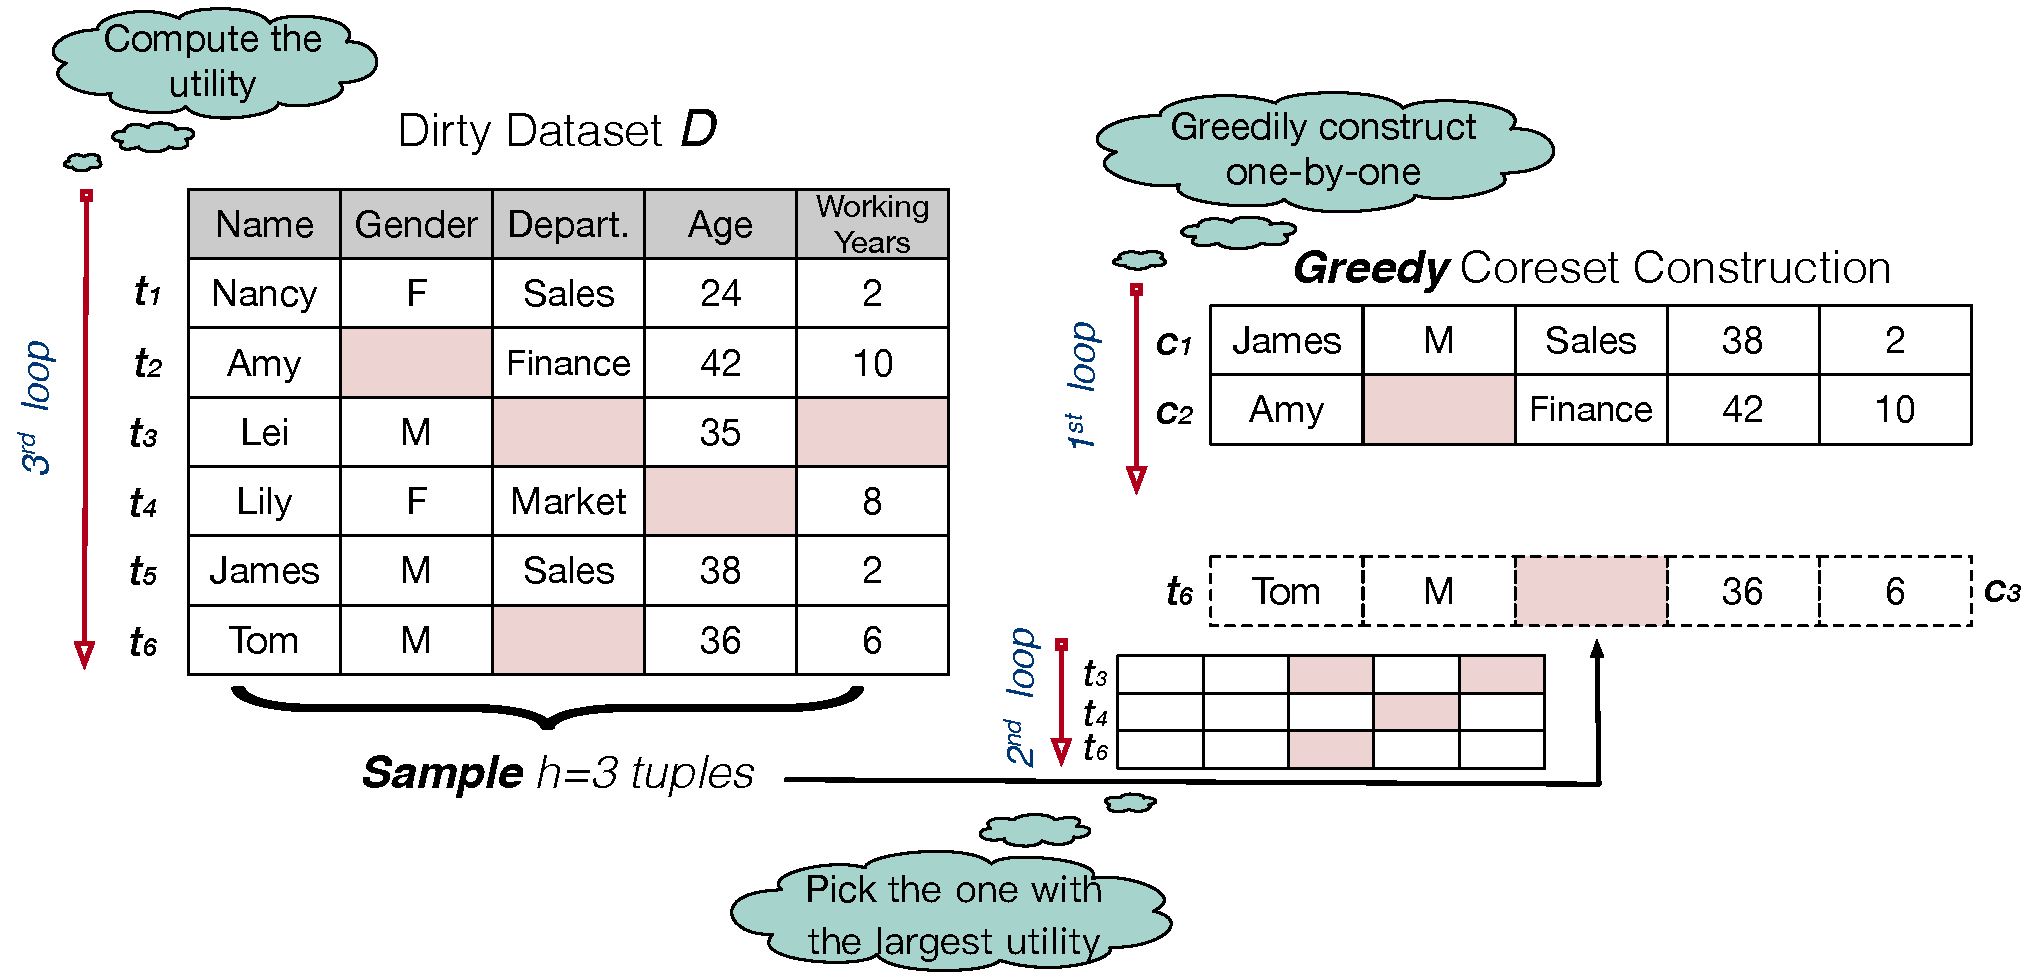
\includegraphics[width=0.6\textwidth]{figs/Overview}
%	\vspace{-2.5em}
	\caption{The \ours framework.}
	\label{fig:overview}
%	\vspace{-2em}
\end{figure}


Next, we will introduce our proposed \ours framework   to solve  Eq.~\ref{eqa:expectation}, which  is non-trivial because it  is NP-hard.
But fortunately, we prove that it has the sub-modular property (see Section~\ref{sec:without}). Hence, \ours uses a greedy framework with three loops to solve the problem with an approximate ratio. 

At a high level, the greedy strategy adds one tuple with the largest ``utility'' to the coreset iteratively, which can be considered as the first loop. In each iteration, we have to iterate tuples in $\train$ to select the one with the largest utility, which is the second loop. Naturally, we have to compute the utility of each tuple, where all tuples in  $\train$ have to be considered, leading to the third loop.
 

Next, we will further illustrate the framework using Figure~\ref{fig:overview} and Algorithm~\ref{alg:framework}.


%!TEX root = ../main.tex

\begin{figure}[!t]
 \vspace{-1em}
	\begin{algorithm}[H]
		\normalem
	\caption{\ours Framework \label{alg:framework}}
		{\small
		\KwIn{Incomplete train data $\train$, coreset size $\numcore$, sample size $h$.}
		\KwOut{A coreset $\core \subseteq \train$, weight $\weightset=\{w_j\}$,$|\core|=|\weightset|=\numcore$.}
		
		$C=\emptyset$;\\\nllabel{alg1:init1}
		
		\While{$|\core|< \numcore$}
		{\nllabel{craig1:loop1}
			
		/*1st loop*/  \\
		
		Sample $h$ tuples as $T_{sample} \subseteq \train \setminus \core$\\\nllabel{craig1:sample}
		
			\For{each tuple $t \in T_{sample}$}  
			{\nllabel{craig1:loop2}
				
				/*2nd loop*/ \\
				
			%	}
			 $\mathrm{E}[t|\core]=\texttt{ComputeUtility}(t, C,D)$;
				 /*3rd loop*/  \\\nllabel{craig1:loop3}
			}		

			$t^*$ = $\argmax_{t\in T_{sample}}\mathrm{E}[t|\core]$ ;\\\nllabel{craig1:maxmulti}
			
			$\core = \core \cup \{t^*\}$;
			\\\nllabel{craig1:add2} 
			
				%\If{$\mathbb{I}[t^*] = 1$}
		%	{ \nllabel{alg:if}
		%		 \cc{Impute $t^*$ (by human or automatic methods).}\\\nllabel{alg:oracle}
		%	
			%}					
		}

	
	    \For{ $t\in \core$} 
	    {\nllabel{craig1:goodcore1}
	       \If{$\mathbb{I}[t] = 1$} {\nllabel{craig1:oracle1}
	         Impute $t$ by a  human or automatic method.\\\nllabel{craig1:oracle}
             }
        }
	 	\For{$j = 1$ to $|\core|$} 
	 	{\nllabel{craig1:cc0}
	 		%$w_j = \sum_{i=1}^{n}\mathbb{I}'[j=\argmin_{c_{j'}\in\core}  %\max\limits_{\hypo\in\vartheta}\lVert \df_i(\hypo) - \df_{\gamma(j')}(\hypo) \rVert ]$;\\\nllabel{craig1:cc}
	 		\For{$i = 1$ to n}
	 		{
	 		  \If{$c_j=\argmin_{c_{j'}\in\core}\max\limits_{\hypo\in\vartheta}\lVert \df_i(\hypo) - \df_{\gamma(j')}(\hypo) \rVert$}
	 		  {
	 		  	$w_j~+\!=~1$;\\\nllabel{craig1:cc}
	 		  }
 		    }
	 		
	 	}
		\Return $\core,\weightset$;\\\nllabel{craig1:return}
		}
	\end{algorithm}
\end{figure}


\stitle{The first loop (lines~\ref{craig1:loop1}-\ref{craig1:add2})} of  the greedy algorithm is  to add the  tuple $t^*$ with the maximum \textit{utility} (\ie $\mathrm{E}[t|\core] = \mathrm{E}[\core] - \mathrm{E}[\core \cup \{t\}]$) into the coreset iteratively for $\numcore$ times. To be specific, the  ``utility''  of a tuple $t$ denotes the reduction of  expectation of GA error after adding $t$  into the coreset $\core$. 

Suppose that $\numcore=3$. Figure~\ref{fig:overview} (the $1^{st}$ loop part) shows the situation that there already have been 2 tuples in $\core$, and we are going to add the third tuple into the coreset.


\stitle{The second loop (lines~\ref{craig1:loop2}-\ref{craig1:loop3})} computes the utilities of  tuples  that are not in coreset $C$, based on which the best one is picked for the first loop. An ideal solution is to consider all tuples in $\train \setminus \core$, which is prohibitively expensive, so in practice we use an efficient method to accelerate
this loop by uniformly sampling $h$ tuples as $T_{sample}$ (line~\ref{craig1:sample}) and then selecting the best one from $T_{sample}$ (line~\ref{craig1:maxmulti}). The  difference is that theoretically, considering all tuples has an approximate ratio 1-$\frac{1}{e}$ (because of the sub-modular property), while the sampling method holds a (1-$\frac{1}{e}-\epsilon$) ratio~\cite{mirzasoleiman2015lazier}, where $\epsilon$ is related to the sampling ratio.

As shown in Figure~\ref{fig:overview}, suppose that $h=3$, and we sample $\{t_3, t_4, t_6\}$ from $\{t_1, t_3, t_4, t_6\}$. Then the second loop iterates the three tuples and computes the utility for each one (the third loop).


\stitle{The third loop (line~\ref{craig1:loop3})} will loop through all tuples in $\train$, so as to compute the utility of tuple $t$ used in the second loop.  To be specific, the core part of the utility computation (\ie \texttt{ComputeUtility}) is to compute $\mathrm{E}[C] = \sum_{k= 1}^{|\worlds|} p_kS_k= \sum_{k= 1}^{|\worlds|} p_k (\sum_{i=1}^n \min_{c_j\in C_k}\dist_{ij})$, from which we can see that it is inevitable to iterate the $n$ tuples in $\train$. However, the most challenging part is that we also have to enumerate a large number of possible worlds. We will illustrate how to solve this in details in Section~\ref{sec:without}.



\stitle{The imputation step (line~\ref{craig1:oracle}).} After \ours selects the coreset $C$ using the above 3 loops, we can leverage a human or automatic method to impute the tuples that are incomplete in $C$, which correspond to Case (5) and Case (6) in Section~\ref{sec:intro} respectively. 




\stitle{Weights computation (lines~\ref{craig1:cc0}-\ref{craig1:cc}).} It computes the weight of each tuple in $C$, which will be used to approximate the full gradient during training. For training, tuples in the coreset are randomly shuffled. Afterwards, suppose that in each step of the gradient decent, when we use $c_j \in \core$ to update the gradient, we compute the gradient $(\df_j)$ of $c_j$ first, and then use $w_j\df_j$ to update the model parameters. $w_j$ is the number of tuples in $\train$ assigned to $c_j$.  The above steps repeat until the model converges.


\stitle{Imputation-in-the-loop optimizations.} Unfortunately, the 3-loop computation of the strategy is rather expensive due to the large number of possible worlds (Section~\ref{sec:without}).   To address this, we can   integrate either human-in-the-loop or the automatic method into \ours framework (Section~\ref{sec:human}).  It iteratively imputes one incomplete tuple or a mini-batch of incomplete tuples. Once the tuple(s) is (are) computed and added to the coreset within the first loop, the number of possible worlds can be significantly reduced, and so does the computational cost. %In addition, how to select an appropriate coreset size $K$ is an important problem, which will be discussed in Section~\ref{exp:sec:end2end}.

%\cc{Do we need to say why this optimization can solve the complexity? But easy to be redundant with Sec 5}

%The advantages of the optimization are two-fold. First, with more and more missing values are imputed, the number of possible worlds are greatly reduced, which reduces the machine cost a lot. Second, for human imputation, it allows us to  gradually impute the tuples accurately, and thus the coreset score computation can be more and more accurate, which produces a better coreset.

\stitle{Group-based acceleration.} As discussed above, we have to iterate all tuples of $D$ in the third loop to compute the utility of a tuple $t$. Given a large train set with missing values, it is still inefficient to compute the coreset. To address this, we propose to assign tuples in $D$ to multiple groups, and use these groups to represent the entire dataset. Since the number of groups are smaller than $n$, the efficiency can be much improved (Section~\ref{sec:group}). 















%!TEX root = ../main.tex






\iffalse
\section{Problem Discussion}

\subsection{Ours}

In Section~\ref{sec:pre}, we have an important mapping $\phi$, \ie $\phi(i) = j, i\in[1,|T|],  j\in[1,|C|]$. $\phi(i) = j$ denotes that we will assign  $t_i$ to $c_j$ and use $\df_{\gamma(j)}$  to represent $\df_i$. Each $t_i$ will be assigned to one and only one $c_j$, but each  $c_j$ might be assigned with multiple tuples in $\train$. 

Consider Eq.~\ref{eqa:expectation}, an important question is how to efficiently compute $\mathrm{E}[\sum_{i\in \train} \min_{j\in \core} d_{ij}]$. Suppose that we first enumerate all possible worlds, then all tuples are deterministic. Thus, we can easily compute
\begin{equation}
	\label{eq:possible_worlds}
	\begin{aligned}
		\mathrm{E}[\sum_{i\in \train} \min_{j\in \core} d_{ij}] & = \sum_{k = 1}^{P} p_{k} * sum_k \\
		& = \sum_{k = 1}^{P} p_{k} * (\sum_{i=1}^{|T|}d_{i, \phi(i)}) \\
		& = \sum_{i=1}^{|T|} \sum_{k = 1}^{P} p_{k} * d_{i, \phi(i)} \\
	\end{aligned}
\end{equation}
where $P$ is the number of possible worlds, $p_{k}$ denotes the probability of occurrence of the $k$-th possible world. Naturally, we have $\sum_{k = 1}^{P} p_{k} = 1$.

Then,  we can aggregate same $d_{i, \phi(i)}$. Suppose we have $d_{g_1}, \cdots, d_{g_C}$. 
\begin{equation}
	\begin{aligned}
		\mathrm{E}[\sum_{i\in \train} \min_{j\in \core} d_{ij}] 
		 = \sum_{i=1}^{|T|} ( &
		 d_{g_1} * (p_{m_1}+\cdots+p_{{m_2} - 1})  \\
		+ & d_{g_2}* (p_{m_2}+\cdots+p_{{m_3} - 1}) \\
		+ & \cdots \\
		+ &  d_{g_C}* (p_{m_C}+\cdots+p_{P}) )
	\end{aligned}
\end{equation}


In practice, we have a reasonable assumption that the imputation of each tuple is independent. For tuple $t_i$, $t_i$ has $\Psi(i)$ imputation schemes and the probability of each scheme is $\rho$.

Every time we compute the utility of a new tuple, we suppose that each tuple in the coreset is already imputed. Then, we have
\begin{equation}
	\begin{aligned}
	\mathrm{E}[\sum_{i\in \train} \min_{j\in \core} d_{ij}] = \sum_{i=1}^{|T|} \sum_{k=1}^{\Psi(i)} \rho_{k} * d_{i, \phi(i)} 
	\end{aligned}
\end{equation}

 
For a new tuple $c$, we suppose that tuple $c$ has a missing value. Consider that $c$ has $\Pi$ different values, \ie $c^{(1)}, \cdots, c^{(\Pi)}$. The probability of each value $c^{(l)}$ is $\pi_{l}$. $\phi_{l}(i)=j$ indicates that when  $c = c^{(l)}$, we assign  $t_i$ to $c_j$.

\begin{equation}
	\mathrm{E}[\sum_{i\in \train} \min_{j\in \core} d_{ij}]  = \sum_{i=1}^{|T|} \sum_{k=1}^{\Psi(i)} \rho_{k} * (\sum_{l=1}^{\Pi} \pi_{l} * d_{i, \phi_{l}(i)}) 
\end{equation}

\subsection{Miao's}

Miao's derivation is similar to ours. 

We assume that for each tuple $x_i$ in $T$, $x_i$ has a corresponding set of tuples $A_i$. Specifically, if there is no missing value in $x_i$, then $x_i$  has been assigned. If there are missing values in $x_i$, then we need to choose a tuple from $A_i$ to replace $x_i$. Similar for tuples in $\core$, each one has a corresponding set $B_i$. Without loss of generality, we can assume that the size of each $A_i$ and $B_i$ is $L$.

Then, we can define a assignment $\varphi: \{x_1, \cdots, x_{|T|}, y_1, \cdots, y_{|\core|}\} \rightarrow \A_1 \times \cdots \times A_{|T|} \times B_1 \times \cdots \times B_{|\core|}$. Then, given an assignment $\varphi$, we can compute the distance between $x_i$ and $y_j$ 
\begin{equation}
	d_{ij}(\varphi) = d[\varphi(x_i), \varphi(y_j)]
\end{equation}
We use $c_i(\varphi) = \min_j d_{ij}(\varphi)$ to denote the minimum distance between $x_i$ and the tuple in $\core$ given the assignment $\varphi$. For each assignment $\varphi$, our goal is to compute $s(\varphi) = c_1(\varphi) + \cdots + c_{|T|}(\varphi)$. 

Apparently, each assignment $\varphi_i$ has a probability $p_i$. Thus, we can rewrite Eq.~\ref{eq:possible_worlds} as 
\begin{equation}
		\begin{aligned}
		\mathrm{E}[\sum_{i\in \train} \min_{j\in \core} d_{ij}] & = \sum_{k = 1}^{P} p_{k} * sum_k \\
		& = \sum_{k = 1}^{P} p_{k} * s(\varphi_k) \\
		& = \sum_{k = 1}^{P} p_{k} * \sum_{i=1}^{|T|} c_i(\varphi_k) \\
		& = S \\
	\end{aligned}
\end{equation}


\begin{figure*}[t]
	\centering
	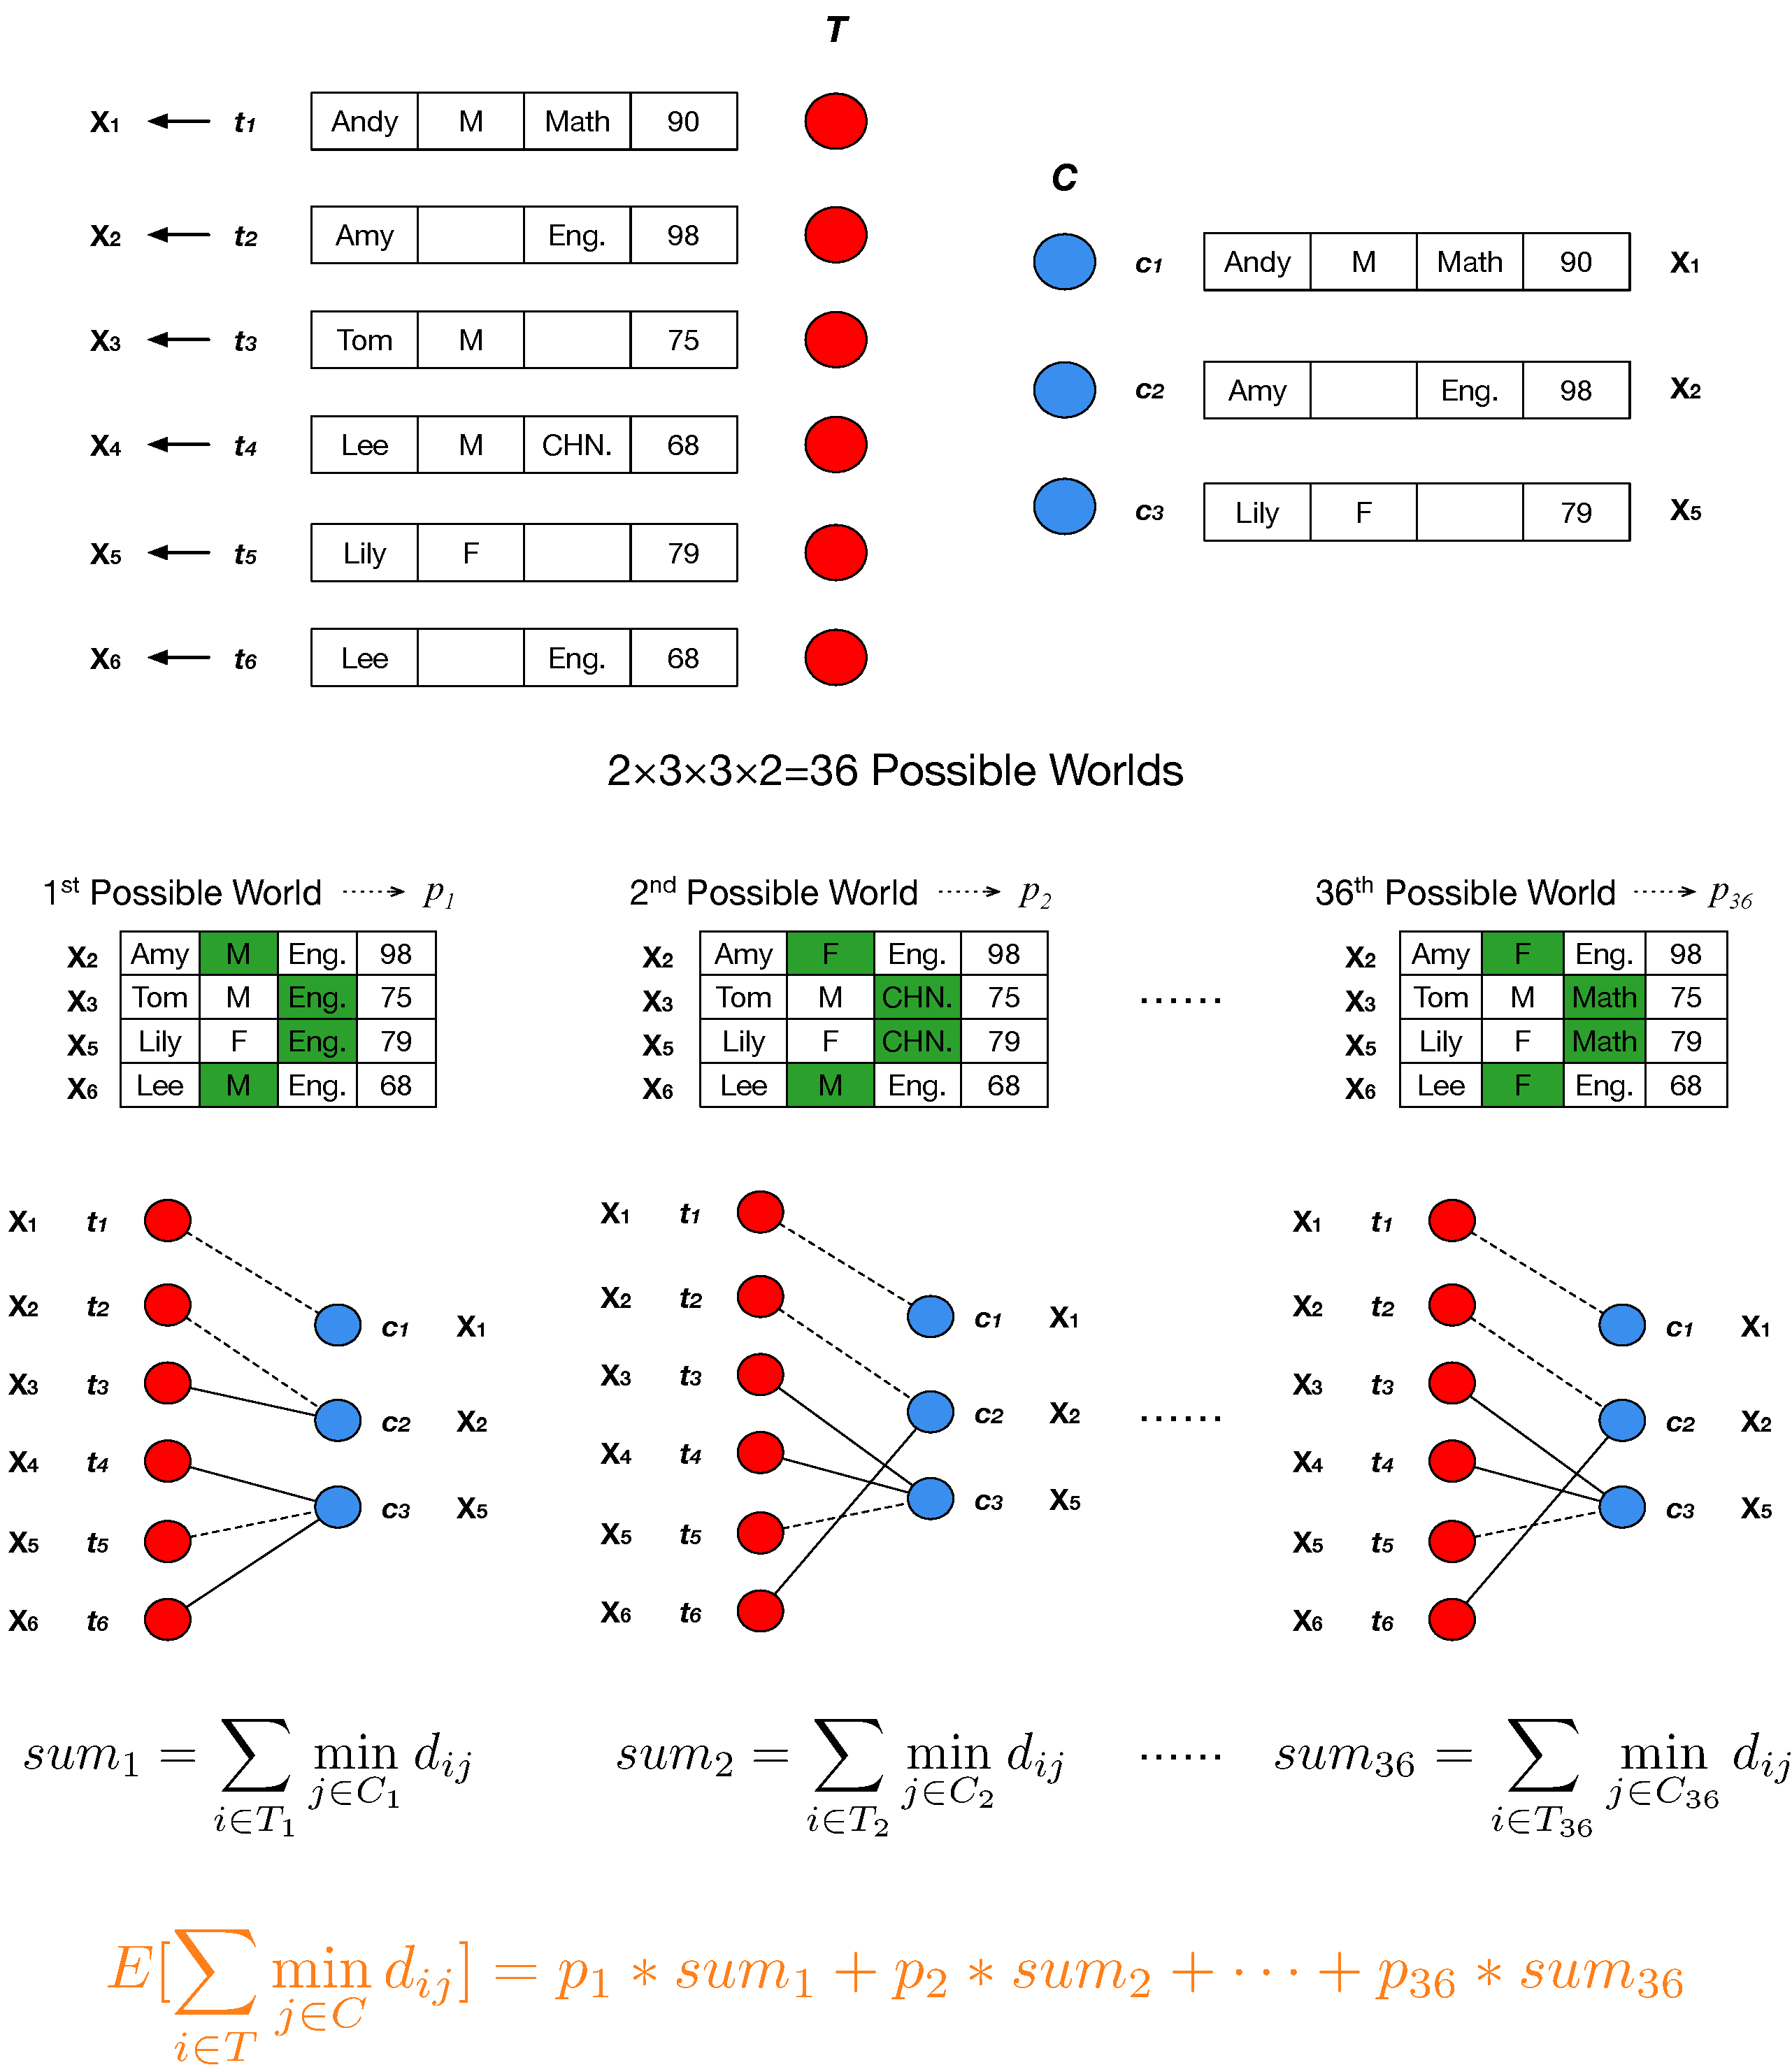
\includegraphics[width=0.98\textwidth]{figs/example.pdf}
	\caption{An example of Coreset4DC.}
	\label{fig:frog}
\end{figure*}
\fi



%!TEX root = ../main.tex
\section{Goodcore Algorithm}
\label{sec:without}

In this section, we will  illustrate \ours algorithm in details for solving Eq.~\ref{eqa:expectation}, which is proven to be prohibitively expensive (Section~\ref{subsec:complexity}).  Then we focus on how to compute the expectation using possible worlds (Section~\ref{subsec:exp}) in the algorithm.

\subsection{Problem Complexity}~\label{subsec:complexity}

Let us first discuss the time complexity of  finding the optimum of Eq.~\ref{eqa:expectation}. 

\begin{theorem}
	\vspace{-0.3em} 
	The problem of expected optimal coreset selection over incomplete data is NP-hard. 
	\vspace{-0.6em} 
\end{theorem}

\begin{proof}
	Let us consider a special case that there is no missing value in $\train$. Our problem becomes the typical coreset selection problem over complete data, which has been proven to be NP-hard by reduction from the Minimum Vertex Cover problem~\cite{dinur2005hardness, mirzasoleiman2020coresets, DBLP:conf/icml/MirzasoleimanBL20}. Hence,  our problem is also NP-hard.
\end{proof}


\begin{theorem}
	\vspace{-0.3em}
	The problem of expected optimal coreset selection over incomplete data has the sub-modular property.
	\vspace{-0.3em}
\end{theorem}

\begin{proof}
	First, we regard $\mathrm{E}[C] = \sum_{k= 1}^{|\worlds|} p_kS_k$ as a utility function, where $S_k = \sum_{i=1}^n \min_{c_j\in C_k}\dist_{ij}$. In fact, $S_k$ can be regarded as a function of the coreset score computation over complete data, which has already  proven to have the sub-modular property~\cite{mirzasoleiman2020coresets, DBLP:conf/icml/MirzasoleimanBL20, killamsetty2021grad}. Therefore, consider the property that a non-negative linear combination of sub-modular functions is also sub-modular~\cite{lin2011class}. To be specific, given   any sub-modular function $g_1,g_2,\ldots,g_k$ and non-negative numbers $\alpha_1,\alpha_2,\ldots,\alpha_k$. Then the function $\mathcal{G}$ defined by $\mathcal{G}=\sum_{i=1}^k \alpha_i g_i$ is sub-modular.
    Hence, we can conclude that our studied problem is a sub-modular problem because $\mathrm{E}[C] = \sum_{k= 1}^{|\worlds|} p_kS_k$, where $p_k>0$.
    \vspace{-0.3em}
\end{proof}

\noindent \textbf{The greedy algorithm.} Given the sub-modular property, naturally, we can design a greedy algorithm with an approximate ratio. As shown in Algorithm~\ref{alg:framework}, we greedily add one tuple to the coreset at each iteration. The added tuple  should have the  largest utility computed by $\mathrm{E}[t|\core] = \mathrm{E}[\core] - \mathrm{E}[\core \cup \{t\}]$. Hence, the key component is that given the original train data $(\train)$ and a coreset ($\core$ or $\core \cup \{t\}$), how to compute the expectation of GA error ($\mathrm{E}[\core]$ or $\mathrm{E}[\core \cup \{t\}]$) of the coreset. However, it is non-trivial because of the large number of possible worlds.  We will first introduce how to compute the probability $p_k$, and describe the expectation computation in Section~\ref{subsec:exp}. After  $K$ tuples are added, we can impute missing tuples in the coreset generated by \ours.


\subsection{Expectation Computation}~\label{subsec:exp}

\noindent \textbf{Possible world probability.} To compute the expectation, it is inevitable to derive the probability of each possible world, which can be taken as a pre-processing step in our framework. 
To be specific, since tuples with missing values are always imputed independently~\cite{miao2022experimental}, given a possible world $\world_k$, the probability $p_k$ can be computed by $p_k = \prod\limits_{t\in \world_k, \mathbb{I}[t] = 1} p_k^t$, where $p_k^t$ denotes the probability of the appearance of tuple $t$ with $\mathbb{I}[t] = 1$. Besides, apparently  $p_k^t = 1$ when $\mathbb{I}[t] = 0$, so $p_k=1$ if there are only complete tuples.
Therefore, our focus is on how to get the value of  $p_k^t$, which can be solved by many approaches, like statistic methods and learning-based methods (see~\cite{miao2022experimental} for a survey). 
%
In this paper, we use the learning-based method~\cite{datawig} with a Python library~\cite{datawigpy} to generate the probability, which can be easily replaced by other libraries or domain-specific methods.
%
%\etitle{Statistic method.} A tuple $t$ may have multiple missing values in different attributes. The straightforward statistic method is to  obtain the probability distribution of values in each attribute through statistic information from $\train$. Afterwards, $p_k^t$ can be computed by simply multiplying the probabilities of these missing values.
%
%\etitle{Deep learning method.}
% Recently, more sophisticated deep learning based methods have been proposed for missing value imputation.
 During training, learning-based methods take $\train$ as input and learn a model $\mathcal{M}$ to describe the joint data distribution.
 For inference,  we have 
$ P(\attr_i | \mathbf{x}, v_{mask}) = \mathcal{M}(\mathbf{x}, v_{mask}, \omega^*)$, where the model takes as input the feature vector $\mathbf{x}$ of $t$, the mask vector $v_{mask}$ (indicating which attributes are missing) and the model parameter $\omega^*$, outputs the probability distribution of a missing attribute $\attr_i$.
 
Suppose that $t$ just  has one missing attribute  $\attr_i$, and then $v_{mask}$ is a one-hot vector with $v_{mask}[i] = 0$. Hence, we can directly obtain $p_k^t$  from the distribution $P(\attr_i | \mathbf{x}, v_{mask})$. For $t$ with multiple missing attributes, we can also compute $p_k^t$ using the chain rule. If $t$ has two missing values of $\attr_i$ and $\attr_j$, to compute $p_k^t$, we have to compute $P(\attr_i, \attr_j | \mathbf{x}, v_{mask})$, abbreviated as $P(\attr_i, \attr_j) = P(\attr_i)P(\attr_j | \attr_i)$. $P(\attr_i)$ can be obtained by masking the $i$-th and $j$-th attribute in $v_{mask}$.
 Then, we only mask the  $j$-th attribute  and impute different values of $\attr_i$ to obtain  $P(\attr_j | \attr_i)$.



 
 %For inference, given a tuple $t$, they leave missing attributes as masks and feed $t$ into the model. Then, the model can directly output the  distribution of missing values and we can obtain the value of  $p_k^t$. 

%\add{which takes an incomplete tuple $t$ along with a mask vector $v_{mask}$ as input and outputs the probability distribution of the missing values. Formally, we have }
%\begin{equation}\label{eq:probDL}
%	P(\attr_i | t, v_{mask}) = M_D(t, v_{mask}, \Omega^*)
%\end{equation}
%\add{where $\attr_i$ denotes the $i$-th attribute and $\Omega^*$ denotes the best parameters of $\mathcal{M}$.}

%\add{We now illustrate how to use $M_D$ to compute the probability of tuple $t$. If there is only one missing value in $t$, suppose $\attr_i$, we can derive the probability distribution using Eq.~\ref{eq:probDL}. We mask the $i$-th attribute (\ie $v_{mask}[i] = 0$) and feed $t$ along with $v_{mask}$ into $M_D$. $M_D$ outputs the probability of different values of $\attr_i$, \ie the probability distribution of $\attr_i$, denoted by $P(\attr_i)$. Apparently,  $P(t) = P(\attr_i)$.}

%\add{Consider that $t$ has two missing values $\attr_i$ and $\attr_j$. It is evident that the probability distribution of $t$ is the joint probability distribution of $\attr_i$ and $\attr_j$, \ie $P(t) = P(\attr_i, \attr_j)$. Then, we have $P(t) = P(\attr_i, \attr_j) = P(\attr_i)P(\attr_j | \attr_i)$. Following Eq.~\ref{eq:probDL}, we can first mask $\attr_i$, $\attr_j$ and obtain the probability distribution $P(\attr_i)$. Then, we only mask $\attr_j$ and impute different values of $\attr_i$ to obtain the marginal probability distribution $P(\attr_j | \attr_i)$. Finally, we multiple $P(\attr_i)$ and $P(\attr_j | \attr_i)$ to compute the probability of $t$. If $t$ has three or more missing values, we can use the chain rule to compute the probability. }



%\add{To be specific, suppose that we have a trained deep learning model $M_D$, which takes an incomplete tuple $t$ along with a mask vector $v_m$ as input and outputs the probability distribution of the missing values. For example, consider that we have a tuple $t$, $t[a] = \texttt{Null}$ and $t[b] = \texttt{Null}$. The range of $a$ and $b$ are $\{1,2\}$ and $\{F,M\}$, respectively. We first feed $t$ with masked attribute $a$ and $b$ into $M_D$. We can obtain the probability distribution of attribute $a$. Suppose that $p(t[a] = 1) = 0.6$ and $p(t[a] = 2) = 0.4$. Then, we can obtain two possible tuples $t[a = 1]$ and $t[a = 2]$. After feeding them into $M_D$, we can get the marginal probability distribution of attribute $b$. Suppose that $p(t[b] = F | t[a] = 1 ) = 0.5$, $p(t[b] = M | t[a] = 1) = 0.5$, $p(t[b] = F | t[a] = 2) = 0.8$ and $p(t[b] = M | t[a] = 2) = 0.2$. Then, we can get the probability distribution of tuple $t$ by multiple the marginal probability distribution of attribute $a$ and $b$, \ie $p(t[a] = 1, t[b] = F) = 0.3$, $p(t[a] = 1, t[b] = M) = 0.3$, $p(t[a] = 2, t[b] = F) = 0.32$ and $p(t[a] = 2, t[b] = M) = 0.08$. For the tuples with more two missing values, we can use the chain rule to solve this problem.}

\begin{example}
	In Figure~\ref{fig:missing}(a), suppose that for the first possible world, we have to compute $p_1 = p_1^2 \times  p_1^3 \times  p_1^4 \times  p_1^6$. For instance, to compute $p_1^3$, given the trained deep learning model, we feed 
	$\{\texttt{Lei}, \texttt{M}, \texttt{Mask}, \texttt{35}, \texttt{Mask}\}$ and a one-hot vector $\{1,1,0,1,0\}$  into the model and compute the probability distribution of this tuple, from which we can get $p_1^3$, \ie the probability of 	$\{\texttt{Lei}, \texttt{M}, \texttt{Sales}, \texttt{35}, \texttt{1}\}$.
	%which is the multiplication result of the probabilities of 
%	\vspace{-0.3em}
\end{example}


\begin{figure}[t]
 \centering
 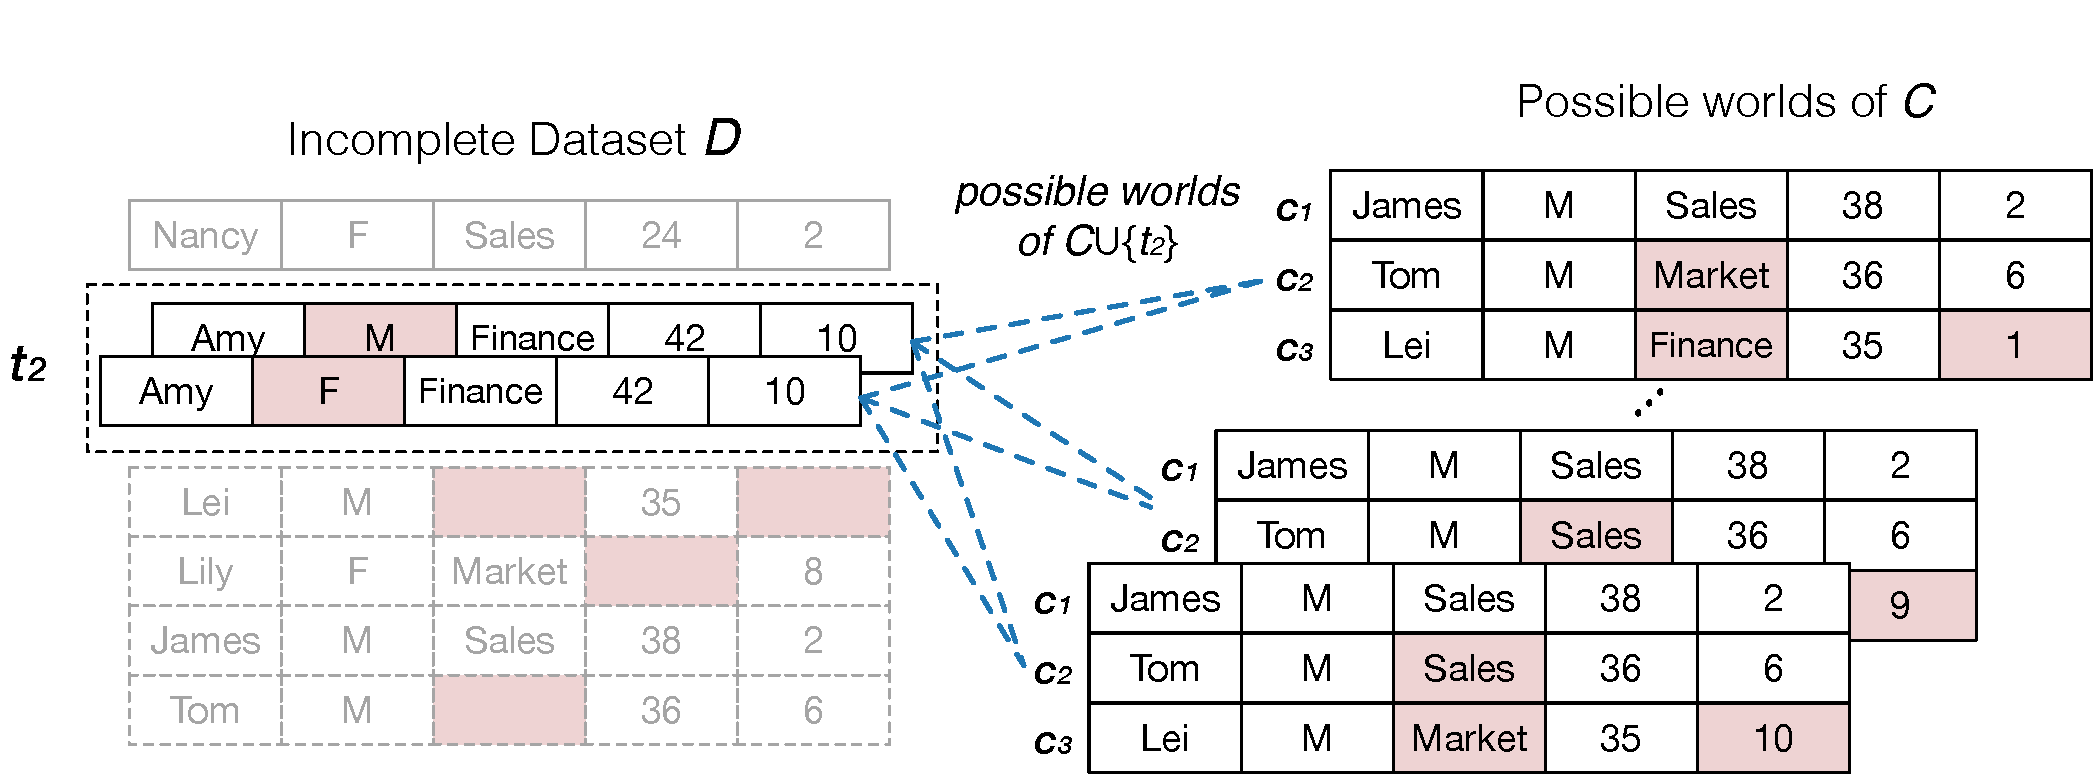
\includegraphics[width=0.6\textwidth]{figs/expectation}
% \vspace{-2.5em}
 \caption{Tuple-based expectation computation.}
 \label{fig:expectation}
% \vspace{-1.5em}
\end{figure}

Compared with statistical approaches, deep learning-based methods use more powerful models with good learning capacity and consider the correlation between attributes. For practitioners, they can use any ad-hoc method to compute the probability.



\stitle{Brute-force expectation computation.} Recap that $\mathrm{E}[C] = \sum_{k= 1}^{|\worlds|} p_k (\sum_{i=1}^n \min_{c_j\in C_k}\dist_{ij})$. Intuitively, the brute-force method is to enumerate each possible world, compute the probability and finally get the expectation. However, there are a huge number of possible worlds, which makes the  computation prohibitively expensive. Specifically, we assume the attribute number $M$ and $|\attr_m|, m\in [1, M]$ are  constants, so the number of possible worlds of each tuple is a constant, denoted by $L$.
Suppose that the number of tuples with missing values is $O(n)$, so the number of possible worlds ($|\worlds|$) is $O(L^n)$. Given a coreset $\core$, the time complexity to compute $\mathrm{E}[C]$ is $O(nL^n)$, which is rather expensive.

\stitle{Tuple-based expectation computation.} To further elaborate, we can easily expand $\mathrm{E}[C]$ as follows:

\vspace{-0.5em}
\begin{equation*}
\begin{aligned}
	\mathrm{E}[C] =& \uwave{p_1(\min_{c_j\in C_1}s_{1j}} + \min_{c_j\in C_1}s_{2j} + \cdots + \min_{c_j\in C_1}s_{nj})\\
	+ ~& \uwave{p_2(\min_{c_j\in C_2}s_{1j}} + \min_{c_j\in C_2}s_{2j} + \cdots + \min_{c_j\in C_2}s_{nj})+ \cdots \\
	+ ~& \uwave{p_{|\worlds|}(\min_{c_j\in C_{|\worlds|}}s_{1j}} + \min_{c_j\in C_{|\worlds|}}s_{2j} + \cdots + \min_{c_j\in C_{|\worlds|}}s_{nj}).
\end{aligned}
\end{equation*}

\noindent  We can see from the above equation that these underlined terms are only related to $t_1\in \train$ as well as  $\{\core_1, \core_2, \cdots, \core_{|\worlds|}\}$, \ie the coresets corresponding to the $|\worlds|$  possible worlds.
However, as the coreset $\core$ is much smaller than the full data $\train$, the number of possible worlds of $\core$ will be also much smaller than $|\worlds|$, and thus there will be many duplicates among $\{\core_1, \core_2, \cdots, \core_{|\worlds|}\}$.
Therefore, many of these underlined terms  have identical variable parts, \ie $\min_{c_j\in C_k} s_{1j}$, when they are associated with the same  $C_k$. These terms are \textit{like terms}. Combining these like terms  (\ie $\sum_{k=1}^{|\worlds|} p_k \min_{c_j\in C_k}s_{1j}$), we can get the expectation of $\min_{c_j\in C}s_{1j}$, denoted by $\mathrm{E}[\min_{c_j\in C}s_{1j}]$.




In short, we can convert the expectation computation over the possible worlds of the entire training set $\train$ to the sum of expectation of each tuple in $\train$, as follows:

\vspace{-0.5em}
\begin{equation}\label{eqa:tuple}
	\mathrm{E}[C] = \sum_{k= 1}^{|\worlds|} p_k (\sum_{i=1}^n \min_{c_j\in C_k}\dist_{ij})= \sum_{i=1}^n \mathrm{E}[\min_{c_j\in C}s_{ij}]
\end{equation}

\begin{example}
	Figure~\ref{fig:expectation} shows how to compute $\mathrm{E}[\min_{c_j\in C}s_{2j}]$. Instead of enumerating $|\worlds|$ possible worlds by the brute-force method, we can enumerate a much smaller number of possible worlds of $\core \cup t_2$, compute the corresponding probabilities and finally get the tuple expectation. Specifically, The left part of Figure~\ref{fig:expectation} shows the possible worlds of the tuple,  the right part shows the possible worlds of the coreset, and their combination is the possible worlds of $\core \cup t_2$. Then, following Eq.~\ref{eqa:tuple}, we can iterate the tuples in $\train$, compute their expectations and sum them up to derive $\mathrm{E}[C]$.
\end{example}




\iffalse
\vspace{-1em}
\begin{equation}\label{equation:triangle}
\begin{aligned}
&  \lVert\sum\limits_{i=1}^N \left( \df_i^+(\hypo) - \df_{\gamma(\map(i))}^+(\hypo) \right) \rVert 
\\
= &\lVert\sum_{i=1}^g  
\sum_{k\in G_i} \left(\df^+_k(\hypo) - \df^+_{\gamma(\map(k))}(\hypo) \right) \rVert 
\\
\le & \sum_{i=1}^g  \lVert
\sum_{k\in G_i}\left( \df^+_k(\hypo) - \df^+_{\gamma(\map(k))}(\hypo) \right) \rVert 
\\
\le & \sum_{i=1}^g  |G_i| \max_{k\in G_i}\lVert 
\df^+_k(\hypo) - \df^+_{\gamma(\map(k))}(\hypo)  \rVert \\
\end{aligned}
\end{equation}
\vspace{-.5em}
\fi

\stitle{Time complexity.} Since the coreset size is $K$, and  the number of tuples with missing values in the coreset is $O(K)$, the time complexity of computing $\mathrm{E}[C]$ using tuple-based method is $O(nL^K)$, where $K$ is much smaller than $n$, compared with the brute-force method. However, note that computing $\mathrm{E}[C]$ is just the third loop in the entire framework. Besides, the first two loops incrementally add $K$ tuples into the coreset, and sample $h$ tuples for tuple selection respectively. Hence, the overall time complexity of coreset selection over incomplete data is $O(KhnL^K)$, which is still expensive when $K$ is not small enough.  
In the next section, we involve the imputation-in-the-loop strategies to achieve further improvement.








%!TEX root = ../main.tex
\section{Optimized Goodcore with Imputation-in-the-loop}
\label{sec:human}


As discussed above, it is rather expensive to directly compute all the $K$ tuples in the coreset.  Hence, in this section, we propose to involve the imputation-in-the-loop mechanism that asks the human, \ie Case (7), or automatic method, \ie Case (8) to impute these missing values iteratively while they are generated by Algorithm~\ref{alg:framework}.


The advantages of this optimization are two-fold. First, with more and more missing values being imputed, the number of possible worlds is greatly reduced, which reduces the machine cost a lot. Second, for human-in-the-loop imputation, it allows us to  gradually impute the tuples accurately, and thus the coreset score computation can be more and more accurate, which produces a better coreset.

 %At a high level, there are two advantages of the human-in-the-loop strategy. On the one hand, in each iteration, the number of possible world is greatly reduced, and thus the time complexity is much lower. On the other hand, as the human has imputed values in previous iterations,  the coreset score computation will be more accurate for the following iterations. That is, the human-in-the-loop strategy continuously improves the accuracy of measuring a coreset using the score, which apparently helps to generate a  better coreset. Next, we  discuss how to  impute one tuple per iteration and impute a small batch of  tuples per iteration respectively.

%!TEX root = ../main.tex

 \begin{figure}[!t]
 \vspace{-1em}
	\begin{algorithm}[H]
		\normalem
	\caption{\texttt{ComputeUtility} (3rd-loop to compute $\mathrm{E}[t|\core]$) \label{alg:one}}
		{\small
		\KwIn{Incomplete train data $\train$, current coreset $\core$, a sampled tuple $t$.}
		\KwOut{The expectation $\mathrm{E}[t|\core]$.}
		    $\hat{\core} = \core \cup \{t\}$;\\\nllabel{one:initc}
		    $\mathrm{E}[\hat{\core}] = 0$; \\\nllabel{one:inite}
			\For{ each tuple $t_i \in \train$} 
			{\nllabel{one:loop}    
                \If{$\mathbb{I}[t]$ = 0 and $\mathbb{I}[t_i]$ = 0  \nllabel{one:clean}} 
                {
                   $\mathrm{E}[\hat{\core}] +\!\!= \min_{c_j\in \hat{\core}}\dist_{ij}$;\\\nllabel{one:cleansum}
                }
                \Else 
                {
                	Get the possible worlds of $\hat{\core} \cup \{t_i\}$;\\\nllabel{one:enumw}
                	Compute $\mathrm{E}[\min_{c_j\in \hat{\core}}s_{ij}]$ using these possible worlds and their probabilities;\\\nllabel{one:exp4pw}
                	$\mathrm{E}[\hat{\core}] +\!\!= \mathrm{E}[\min_{c_j\in \hat{\core}}s_{ij}]$;\\\nllabel{one:dirtysum}
                } 
			}	
		
	 	$\mathrm{E}[t|\core] = \mathrm{E}[\core] - \mathrm{E}[\hat{\core}]$;\\\nllabel{one:expt}
		\Return $\mathrm{E}[t|\core]$;\\\nllabel{one:return}
		}
	\end{algorithm}
\end{figure}

	%\nllabel{craig:sample}\nllabel{alg:maxmulti} 	 \nllabel{alg:add2} \nllabel{alg:if}	\nllabel{alg:oracle}

\subsection{One Tuple Each Iteration}~\label{subsec:one}



In fact, we can just slightly modify Algorithm~\ref{alg:framework} to  achieve the imputation-in-the-loop strategy.
To be specific,  in the first loop, we will iteratively impute the tuple   once an incomplete  tuple $t^*$ is computed by \ours, rather than conducting the imputation after $K$ tuples are computed, as discussed in Section~\ref{sec:without}. To this end, we move the imputation step (lines~\ref{craig1:oracle1}-\ref{craig1:oracle} in Algorithm 1) inside the first loop of Algorthm 1, \ie imputing each selected $t^{*}$ by a human or automatic method in each iteration after line~\ref{craig1:add2}.




Afterwards, we will add the next tuple into the coreset, so another loop starts and $h$ tuples are sampled. In the following, we will expand the third loop,   \ie the function \texttt{ComputeUtility} (line~\ref{craig1:loop3})  of Algorithm~\ref{alg:framework} under this one tuple per iteration scenario. 




As shown in Algorithm~\ref{alg:one}, at the beginning, we temporarily add the sampled tuple $t$ to the current coreset, so as to compute the benefit of $t$, \ie  $\mathrm{E}[t|\core]$. To this end, we have to first  compute the expectation  of GA error bound of $\hat{\core}$   (\ie computing $\mathrm{E}[\hat{\core}]$ in the for-loop lines~\ref{one:loop}-\ref{one:dirtysum}). And the expectation \wrt $\core$ (\ie $\mathrm{E}[\core]$) has been computed in the last loop. Then we can compute $\mathrm{E}[t|\core] = \mathrm{E}[\core] - \mathrm{E}[\hat{\core}]$ (line~\ref{one:expt}).


Specifically, to compute $\mathrm{E}[\hat{\core}]$, we will use the tuple-based expectation computation method proposed in Section~\ref{subsec:exp}. For each tuple $t_i\in \train$, if $t_i$ and $t$ are both complete, we can directly compute $\min_{c_j\in \hat{\core}}s_{ij}$ because there is no incomplete data in $\hat{\core}$ (lines~\ref{one:clean}-\ref{one:cleansum}). Otherwise, we will enumerate the possible worlds of $\hat{\core} \cup \{t_i\}$, compute their probabilities and compute $\mathrm{E}[\min_{c_j\in \hat{\core}}s_{ij}]$
 (lines~\ref{one:enumw}-\ref{one:exp4pw}).
  Note that since there are at most two tuples (\ie $t_i$ and $t$) have missing values, the number of possible worlds is small because other missing values in $\hat{\core}$ have been imputed by humans in previous iterations.

\stitle{Time complexity analysis.} As discussed above, using this human-in-the-loop strategy, the number of possible worlds to be considered is greatly reduced. For   Algorithm~\ref{alg:one}, the time complexity is $O(nL^2)$ because there are at most two incomplete tuples in $\hat{\core}$. For the entire three loops framework, the time complexity is  $O(KhnL^2)$, which is much lower  than the solution without imputation in the loop.
  
  However,  if we utilize the human for imputation, the above method  will incorporate many human iterations. In the following,  we propose to ask human to impute a small batch of missing tuples in each iteration, so as to reduce the  number of human iterations.
  

% we initialize the temporary coreset $\core'$ by combining current coreset $\core$ and the sampled tuple $t$ (line~\ref{one:initc}). We also initialize the expectation of $\core'$ as 0 (line~\ref{one:inite}). Then, for each tuple $t_i$ in $\train$, we update the expectation of $t_i$ (line~\ref{one:clean}-\ref{one:dirtysum}). If $t$ and $t_i$ are both complete tuples, we can easily update the expectation without enumerate the possible worlds (line~\ref{one:cleansum}). Otherwise, we first need to enumerate the possible worlds of  $\core' \cup \{t_i\}$ (line~\ref{one:enumw}) and then compute the expectation of $t_i$ in  different possible worlds (line~\ref{one:exp4pw}-\ref{one:dirtysum}). Finally, we can compute the utility of $t$ by comparing the expectation between $\core$ and $\core'$ (line~\ref{one:expt}).



%!TEX root = ../main.tex

 \begin{figure}[!t]
 \vspace{-1em}
	\begin{algorithm}[H]
		\normalem
	\caption{Batch algorithm of \ours~\label{alg:batch}}
		{\small
			\KwIn{$\train$, $\numcore$, $h$, batch size $b$.}
			\KwOut{A coreset $\core$, weight $\weightset$.}
			
			$C=\emptyset$, $cnt = 0$;\\\nllabel{batch:batchinit1}
			
			\While{$|\core|< \numcore$}
			{\nllabel{batch:batchloop1}
				
				%/*1st loop*/ \\
				Sample $h$ tuples as $T_{sample} \subseteq \train \setminus \core$\\\nllabel{batch:sample}
				\For{ each tuple $t \in T_{sample}$} 
				{\nllabel{batch:loop2}
					%/*2nd loop*/ 
					
					%	}
				$\mathrm{E}[t|\core]=\texttt{ComputeUtility}(t, C,D)$;\\\nllabel{batch:loop3}% /*3rd loop*/  
			}		
			
			$t^*$ = $\argmax_{t\in T_{sample}}\mathrm{E}[t|\core]$ ;\\\nllabel{batch:maxmulti}
			
			$\core = \core \cup \{t^*\}$; \\\nllabel{batch:addcoreset}
			
			\If{$\mathbb{I}[t^*] = 1$}
			{ \nllabel{batch:ifincomp}
				$cnt++$; \\\nllabel{batch:batchadd}
			}
			
			\If{$cnt = b$}
			{\nllabel{batch:batchenough}
				Ask the human to impute the incomplete tuples;\\\nllabel{batch:batchoracle}
				$cnt = 0$; \\\nllabel{batch:batchzero}
			}			
			
		}
	
	 Compute the weight $\weightset$.\\\nllabel{batch:weight}
	\iffalse	\For{$j = 1$ to $|\core|$} 
		{\nllabel{batch:cc0}
			$w_j = \sum_{i=1}^{n}\mathbb{I}[j=\argmin_{c_{j'}\in\core}  \max\limits_{\hypo\in\vartheta}\lVert \df_i(\hypo) - \df_{\gamma(j')}(\hypo) \rVert ]$;\\\nllabel{batch:cc}
		} \fi
		\Return $\core,\weightset$;\\\nllabel{batch:batchreturn}
		}
	\end{algorithm}
\vspace{-2em}
\end{figure}

\subsection{One Batch Each Iteration with Human-in-the-loop}
\label{subsec:batch}

In Section~\ref{subsec:one}, one  tuple per iteration by humans  requires many human iterations. However, if we just incorporate a single human iteration like Section~\ref{subsec:exp}, it is infeasible to compute the tuples to be imputed due to the large number of possible worlds. Therefore, in this subsection, we propose a trade-off solution that asks the human to impute a small batch of tuples per human iteration.

To be specific, as shown in Algorithm~\ref{alg:batch}, compared with the one tuple per human iteration algorithm (\ie the modified Algorithm~\ref{alg:framework} at the beginning of Section ~\ref{subsec:one}), we additionally take the batch size $b$ as input (when $b=1$, Algorithm~\ref{alg:batch} is in fact the modified Algorithm~\ref{alg:framework}). Algorithm~\ref{alg:batch} also incorporates 3 loops, but the main difference is that we do not instantly ask the human to impute the most beneficial tuple $t^*$ among $T_{sample}$. Instead, we just add $t^*$ into the coreset $\core$ (line~\ref{batch:addcoreset}). When there have been $b$ incomplete tuples, we ask the human to impute these tuples together (line~\ref{batch:batchenough}-\ref{batch:batchzero}). Finally we compute the weight (line~\ref{batch:weight}), same as  Algorithm~\ref{alg:framework}.  Although this approach reduces the number of human iterations, it takes a longer time to compute $\mathrm{E}[t|\core]$ (line~\ref{batch:loop3}) than Algorithm~\ref{alg:framework} because there are more incomplete tuples, which indicates more possible worlds. Specifically, the time complexity of computing $\mathrm{E}[t|\core]$ is $O(nL^b)$, which is also expensive. Hence, we propose a heuristic method to accelerate this process as follows. 

\stitle{Reducing the number of possible worlds.} 
A straightforward method of improving the efficiency is to reduce the number of possible worlds. To this end, intuitively, we should focus more on the possible world with a high probability, so these possible worlds with low probabilities can be pruned without sacrificing the accuracy of expectation computation much. Note that for each possible world, the probability is computed by the multiplication of the probabilities of incomplete tuples in the  world because the tuples can be considered independent~\cite{miao2022experimental}. Therefore,  we can remove the possible worlds of each tuple with low probabilities (\ie  reducing $L$), and thus the number of possible worlds of the entire coreset is greatly reduced. 
For example, we can keep top-$l$ (\eg $l=3$) possible worlds (\ie 3 different possible imputations of $t$ with high probabilities) of a tuple $t$. Then for the batch of $b$ incomplete tuples, the number of possible worlds is $l^b$ and the complexity of computing $\mathrm{E}[t|\core]$ is $O(nl^b)$, where both $l$ and $b$ are small enough. Overall, the time complexity is $O(Khnl^b)$. Besides, we can also apply this heuristic method to make the algorithm in Section~\ref{sec:without} practical, which is evaluated in Section~\ref{exp:sec:batchalgo}.






%Recap that in Algorithm~\ref{alg:one}, we need to enumerate the possible worlds of current coreset $\core'$ to compute the benefit of $t$. If the number of possible of each individual tuple (\ie $L$) is large, enumerating all the possible worlds of $\core'$ takes a lot of time since the number is exponential. 

%Then, a straightforward method is to reduce the number of possible worlds of each individual tuple. For example, if every tuple has only 3 possible worlds, the time cost of enumerating the possible worlds for $\core'$ is acceptable. Fortunately, only the possible worlds with high probability of each tuple have a great impact on the computation of benefit. In other words, the possible worlds with low probability could be ignored. Therefore, we propose to use the $top$-$l$ tuples with the largest probability of each tuple when enumerating the possible worlds for $\core'$. To be specific, we only keep the $top$-$l$ tuples with the highest probability for each tuple. Then, only these $top$-$l$ tuples are used in our algorithm. Thus, the complexity of computing $\mathrm{E}[t|\core]$ is $O(nl^b)$, where both $l$ and $b$ are small enough.





















%!TEX root = ../main.tex
\subsection{Convergence Rate Analysis}
\label{sec:proof}

Convergence rate is often used to reflect the speed of finding the optimal parameters for the machine learning algorithm. With a higher convergence rate, we can take fewer epochs to make the model converge. To compute the convergence rate, we have  to compute the distance between the parameter $\hypo$ and the optimal parameter $\hypo^*$ in the $t$-th and the $(t+1)$-th epoch. Since $\fun$ is a strongly convex function, $\forall \hypo, \hypo^{\prime}$ we have

\vspace{-0.5em}
\begin{equation}
	\label{eq:convex}
	\small
	\fun(\hypo) - \fun(\hypo^{\prime}) \ge  \nabla \fun(\hypo^{\prime}) (\hypo - \hypo^{\prime}) + \frac{\eta}{2} \Vert \hypo - \hypo^{\prime} \Vert^{2}
\end{equation}


\noindent where $\eta$ is a constant.  We denote the stepsize as $\zeta_t = \frac{\zeta_0}{k^\tau}$ for the $t$-th epoch, where $\tau$ is a constant.
%Then, we have $max_{\hypo \in \vartheta}  \Vert \df_i(\hypo) - \df_{j}(\hypo) \Vert \leq max_{\hypo \in \vartheta}  \Vert \df_i(\hypo) - \sum_{k= 1}^{|\worlds|} p_k (\df_{j \in \core_k}(\hypo)) \Vert$ .  
%In Section~\ref{sec:pre},  the gradient approximate error can be bounded, \ie $\forall  i, j, \max\limits_{\hypo\in\vartheta}\lVert \df_i(\hypo) - \df_j(\hypo) \rVert \le \epsilon$. 
After using gradient descent in each step, we have $\Vert \hypo^{t+1} - \hypo^{*} \Vert^{2} 
= \Vert \hypo^{t} - \zeta_{k} \sum_{j=1}^{\vert \core \vert} w_j \nabla \fun_{\gamma(j)} (\hypo_{j-1}^t) - \hypo^{*} \Vert^{2}$. Then, following Eq.~\ref{eq:convex}, we have 

\vspace{-1em}
\begin{equation}
	\label{eq:afterig}
	\small
	\begin{aligned}
		\Vert \hypo^{t+1} - \hypo^{*} \Vert^{2} 
		\le  \Vert \hypo^{t} - \hypo^{*} \Vert^{2} - 2 \zeta_{t} \sum_{j=1}^{\vert \core \vert} (\fun_{j}(\hypo^{t}) - \fun_{j}(\hypo^{*}))  \\
		+ 2 \zeta_{t} \sum_{j=1}^{\vert \core \vert} (\fun_{j}(\hypo_{j-1}^{t}) 
		- \fun_{j}(\hypo^{t})) + \zeta_{t}^{2} \sum_{j=1}^{\vert \core \vert} \Vert w_{j} \nabla \fun_j (\hypo_{j-1}^t) \Vert^{2}
	\end{aligned}
\end{equation}



Recap that we select a coreset that minimizes $\mathrm{E}[C]$ through converting gradient difference to feature distance ($s_{ij}$) computation. Obviously, given a dataset, $s_{ij}$ can be bounded (suppose that $s_{ij} \leq s_{0}$). Then we have
$\mathrm{E}[\min_{c_j\in C}s_{ij}] = \sum_{k= 1}^{|\worlds|} p_k (\min_{c_j\in C_k}\dist_{ij}) \leq \sum_{k= 1}^{|\worlds|} p_k * s_{0} = s_{0}$, and thus  $\mathrm{E}[C] = \sum_{i=1}^n \mathrm{E}[\min_{c_j\in C}s_{ij}] \leq n * s_{0} = \kappa_1$. Besides, we also have $max_{\hypo \in \vartheta} \Vert \sum_{i=1}^{n} \nabla \fun_{i}(\hypo) - \sum_{j=1}^{\vert \core \vert} w_j \nabla \fun_{\gamma(j)}(\hypo) \Vert \leq \sum\limits_{i=1}^n \min \limits_{c_j\in\core}\lVert \df_i(\hypo) - \df_{\gamma(j)}(\hypo) \rVert \leq \sum\limits_{i=1}^n \min \limits_{c_j\in\core} \dist_{ij}  \leq \kappa_1$.
%Thus, given a coreset $\core$, $\sum\limits_{i=1}^n \min \limits_{c_j\in\core} \dist_{ij}  \leq \sum\limits_{i=1}^n s_{0} \leq n * s_{0} = \kappa_0$.Apparently, we have $\kappa_0 = \kappa_1$. Then, we have $max_{\hypo \in \vartheta} \Vert \sum_{i=1}^{n} \nabla \fun_{i}(\hypo) - \sum_{j=1}^{\vert \core \vert} w_j \nabla \fun_{\gamma(j)}(\hypo) \Vert \leq \sum\limits_{i=1}^n \min \limits_{c_j\in\core}\lVert \df_i(\hypo) - \df_{\gamma(j)}(\hypo) \rVert \leq \sum\limits_{i=1}^n \min \limits_{c_j\in\core}\lVert \dist_{ij} \rVert \leq \kappa_1$. In addition, we use incremental gradient method in Algorithm~\ref{alg:framework}, we have $\Vert \hypo_t - \hypo^{*} \Vert \le \kappa_2$.
Following the definition of  convex function,  we have $\fun_{j}(\hypo^{t}) - \fun_{j}(\hypo^{*}) \leq w_j \nabla \fun_{j}(\hypo^{*})(\hypo^{t} - \hypo^{*}) + \frac{\eta}{2} \Vert \hypo^{t} - \hypo^{*} \Vert^{2}$. Based on the above things, we can apply Cauchy-Schwarz inequlity~\cite{strang2006linear} and derive  

\vspace{-1em}
\begin{equation}
	\label{eq:item1}
	\small
	\begin{aligned}
		& - 2 \zeta_{t} \sum_{j=1}^{\vert \core \vert} (\fun_{j}(\hypo^{t}) - \fun_{j}(\hypo^{*}))  \\
		\le &  - \eta \zeta_{t} \Vert \hypo^{t} - \hypo^{*} \Vert^{2} + 2 \zeta_{t} \Vert \sum_{j=1}^{\vert \core \vert} w_j \nabla \fun_{j}(\hypo^{*}) \Vert \Vert (\hypo^{t} - \hypo^{*}) \Vert \\
		\le & - \eta \zeta^{t} \Vert \hypo^{t} - \hypo^{*} \Vert^{2} + \frac{2 \zeta^{t} \vert \core \vert \kappa_1 \kappa_2}{\eta}  
	\end{aligned}
\end{equation}

\noindent where $\kappa_2$ can be regarded as the upper bound of $\Vert \hypo_t - \hypo^{*} \Vert$.
Since $\fun$ is convex, thus, for item $\fun_{j}(\hypo_{j-1}^{t}) 
- \fun_{j}(\hypo^{t})$, we have $\fun_{j}(\hypo_{j-1}^{t}) 
- \fun_{j}(\hypo^{t}) \leq \Vert w_j \nabla \fun_{j}(\hypo^{t}) \Vert \zeta_t \sum_{i=1}^{j - 1} \Vert w_i \nabla \fun_{i}(\hypo_{i-1}^{t}) \Vert$. In addition, we can assume that $max_{j \in \{ 1, \cdots, \vert \core \vert\}} \Vert \nabla\fun_j(\hypo) \Vert \le \kappa_3$. 
Then, we have

\vspace{-1em}
\begin{equation}
	\label{eq:item2}
	\small
	\begin{aligned}
		& 2 \zeta_{t} \sum_{j=1}^{\vert \core \vert} (\fun_{j}(\hypo_{j-1}^{t}) 
		- \fun_{j}(\hypo^{t})) + \zeta_{t}^{2} \sum_{j=1}^{\vert \core \vert} \Vert w_{j} \nabla \fun_j (\hypo_{j-1}^t) \Vert^{2} \\
		\le & 2 \zeta_{t} \sum_{j=1}^{\vert \core \vert} \Vert w_j \nabla \fun_{j}(\hypo^{t}) \Vert \zeta_t \sum_{i=1}^{j - 1} \Vert w_i \nabla \fun_{i}(\hypo_{i-1}^{t}) \Vert + \zeta_{t}^{2} \sum_{j=1}^{\vert \core \vert} \Vert w_{j} \nabla \fun_j (\hypo_{j-1}^t) \Vert^{2}\\
		\le & 2 \zeta_t^2 (\vert \core \vert^2 - \vert \core \vert) w_{max}^2 \kappa_3^2 + \zeta_t^2 \vert \core \vert w_{max}^2 \kappa_3^2
	\end{aligned}
\end{equation}

Thus, from Eq.~\ref{eq:afterig} to Eq.~\ref{eq:item2}, we can get

\vspace{-0.5em}
\begin{equation}
	\small
	\begin{aligned}
		\Vert \hypo^{t+1} - \hypo^{*} \Vert
		\le  (1 - \eta \zeta_t)\Vert \hypo^{t} - \hypo^{*} \Vert^{2} + \frac{2 \zeta_{t} \vert \core \vert \kappa_1 \kappa_2 }{\eta}  + \zeta_t^2 \vert \core \vert^2 w_{max}^2 \kappa_3^2 
	\end{aligned}
\end{equation}

%Finally, following Lemma 4 in~\cite{chung1954stochastic}, the convergence rate of Algorithm~\ref{alg:framework} is at the same rate of $O(\frac{1}{\sqrt{k}})$ as the  convergence rate for incremental gradient descent on the entire dataset~\cite{nedic2001convergence}.
Finally, following Lemma 4 in~\cite{chung1954stochastic}, the convergence rate of Algorithm~\ref{alg:framework} is at the same rate of $O(\frac{1}{\sqrt{k}})$ as the  convergence rate on the entire dataset~\cite{nedic2001convergence}. Therefore, theoretically, the selected coreset can converge with the same number of epochs as training on the full data. In this way, since  coreset has a much smaller size than the full data, the efficiency can be much improved.
%!TEX root = ../main.tex


\section{Group-based Acceleration}

As discussed above, we can observe that in Section~\ref{subsec:one}, even with the most efficient imputation-in-the-loop  strategy, \ie  one tuple in  each iteration, the time complexity is  $O(KhnL^2)$, where $K$ is the size of the coreset, $h$ is the sample size, $L$ is a small constant and $n$ is the number of entire dataset. Therefore, obviously, the efficiency is dominated by $n$, which is still low when $n$ is large, and thus it  is necessary to further accelerate this process.

\noindent \textbf{Key observation.}   Recap that in Figure~\ref{fig:overviewSingle}, we can observe that  given a tuple $c$ in the coreset, the tuples in the origin full train set $\trainc$ represented by $c$ are likely to be  closer to each other than other tuples not represented by $c$.
Based on this observation, we propose to first cluster the full train set into groups, and then compute the coreset based on these groups. This can achieve much acceleration because the number of groups is much smaller than $n$. 

At the following, we will theoretically and empirically show the groups-based solution can accelerate the coreset selection process without sacrificing the effectiveness much.

%the acceleration can be achieved by clustering the 

\subsection{Group-based Solution Overview}

\begin{figure}[t]
    \centering
    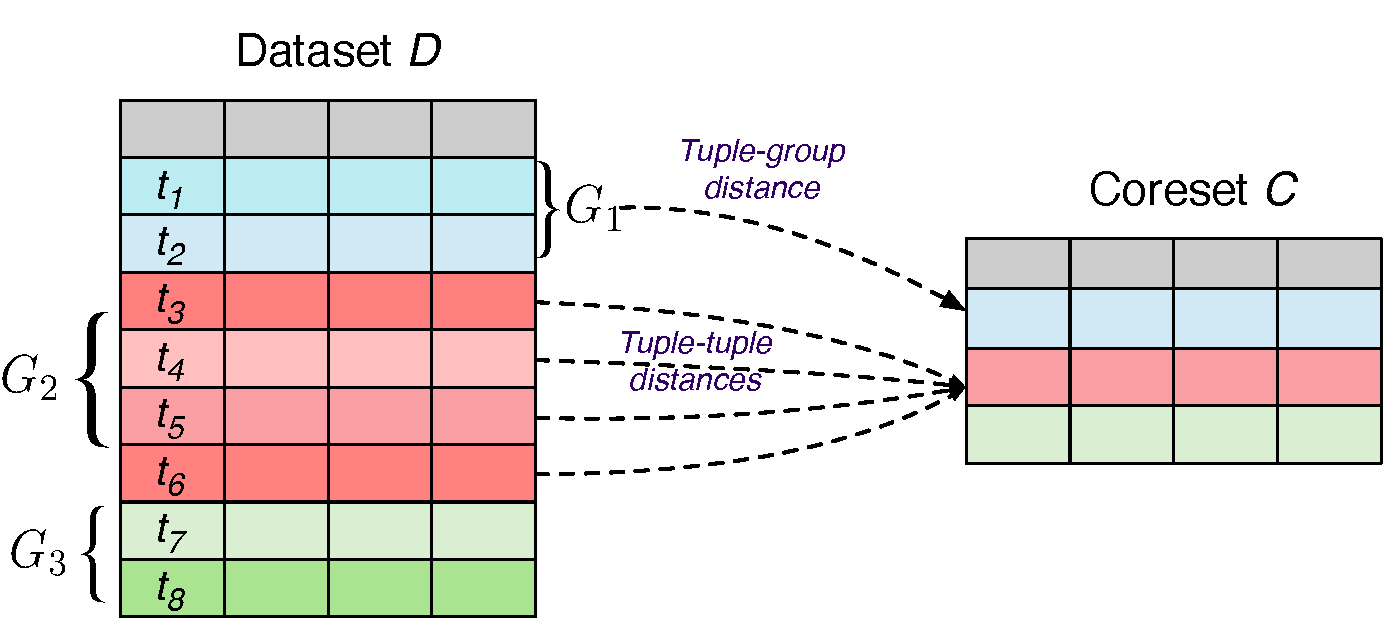
\includegraphics[width=0.6\textwidth]{figs/Overview-gb}
   % \vspace{-2.5em}
    \caption{Illustration of the Group-based Solution.}
    \label{fig:overview-gb}
   % \vspace{-1.5em}
\end{figure}

As shown in Figure~\ref{overview-gb}, one of the core parts of coreset computation is to compute the tuple-tuple distance, \ie $s_{ij}$. For the group-based solution, we just need to consider the relationship between tuples and these pre-computed groups, namely tuple-group distance, rather than the large amount of tuple-tuple distances. As we will discuss below, the computation of tuple-group distance does not need to iterate all tuples in the group, and thus  the overall efficiency can be much improved. 

At a high level, the overall process of group-based \ours solution with imputation in the loop is shown in Algorithm~\ref{alg:group}. To be more explicit, we illustrate Algorithm~\ref{alg:group} in comparison with Algorithm~\ref{alg:framework} in Section~\ref{subsec:framework} without clustering (the modified parts are highlighted in blue fonts).

To be specific, as shown in Line~\ref{alg4:cluster}, we first cluster $\trainc$ into groups using the efficient local sensitive hash (LSH) approach, where each group $\group_u, u\in[1, \groups]$ denotes the indexes of tuples in $\trainc$. In this way, every pair of tuples in the same group is close to each other in the feature distance.
%
 Afterwards, the major difference between group-based \ours and original \ours lies in the 3rd loop. Instead of  selecting a coreset to represent all tuples in the train set, group-based \ours selects a coreset to represent all clusters. As these clusters can well capture the train set distribution, the selected coreset contains enough information to approximate the full gradient of $\trainc$. 
 
 To this end, recap that the typical coreset selection algorithm needs the tuple-tuple distances to approximate the full gradient, while in group-based \ours, we just need to consider the tuple-group distances, \ie  
$\overline{s}_{\gamma(j)u} = \max\limits_{v \in \group_u} s_{\gamma(j)v}, s_{\gamma(j)v} = \lVert\mathbf{x}_v - \mathbf{x}_{\gamma(j)}\rVert, \gamma(j)\in[1, n]$, which denotes the maximum feature distance between the tuple $c_j$ in the coreset and all tuples in $\group_u$. As tuples in $\group_u$ are close to each other, $\overline{s}_{\gamma(j)u}$ can represent the relationship between $c_j$ and tuples in $\group_u$ to a large extent. But as shown in Line~11, we finally use an upper bound $\bound_{jk}$ to compute the coreset score because computing $\overline{s}_{\gamma(j)u}$ needs to iterate the tuples in $\group_u$, which is time-consuming. Next, we will theoretically show that using the upper bound can still derive a bounded GA error, leading to a well-performed coreset. 

%!TEX root = ../main.tex

\begin{figure}[!t]
 \vspace{-1em}
	\begin{algorithm}[H]
		\normalem
	\caption{Group-based \ours Solution (imputation-in-the-loop) \label{alg:group}}
		{\small
			
		\KwIn{Incomplete train data $\train$, coreset size $\numcore$, sample size $h$.}
		
		\KwOut{A coreset $\core \subseteq \train$, weight $\weightset=\{w_j\}$,$|\core|=|\weightset|=\numcore$.}
		
		$C=\emptyset$;\\\nllabel{alg1:init1}
		
		\add{Cluster $\train$ into groups $\groups = \{ \group_1, \group_2, ..., \group_\groupsize \}$;}\\\nllabel{alg4:cluster}
		
		\While{$|\core|< \numcore$}
		{\nllabel{craig1:loop1}
			
		/*1st loop*/  \\
		
		Sample $h$ tuples as $T_{sample} \subseteq \train \setminus \core$\\\nllabel{craig1:sample}
		
			\For{each tuple $t \in T_{sample}$}  
			{\nllabel{craig1:loop2}
				
				/*2nd loop*/ \\
				 $\hat{\core} = \core \cup \{t\}$;\\
			%	}
			 %$\mathrm{E}[t|\core]=\texttt{ComputeUtility}(t, C,D)$;
				 %/*3rd loop*/  \\\nllabel{craig1:loop3}
				 \For{\add{each group $G_k \in \groups$}}  
				 {
				 	\add{/*3rd loop*/} \\
				 
				 	%	Get the possible worlds of $\hat{\core} \cup \{t_i\}$;\\\nllabel{one:enumw}
				 	%	Compute $\mathrm{E}[\min_{c_j\in \hat{\core}}s_{ij}]$ using these possible worlds and their probabilities;\\\nllabel{one:exp4pw}
				 		\add{$\mathrm{E}[\hat{\core}] +\!\!= \mathrm{E}[\min_{c_j\in \hat{\core}}\bound_{jk} \times |\group_k|]$, where $\bound_{jk}$ is the upper bound of} \\\quad \\\nllabel{alg4:bound} \add{$\overline{s}_{\gamma(j)k} = \max\limits_{v \in \group_k} s_{\gamma(j)v}, s_{\gamma(j)v} = \lVert\mathbf{x}_v - \mathbf{x}_{\gamma(j)}\rVert, \gamma(j)\in[1, n]$; }\\\nllabel{one:dirtysum}
			     }
		         \add{$\mathrm{E}[t|\core] = \mathrm{E}[\core] - \mathrm{E}[\hat{\core}];$}
				 
			}		

			$t^*$ = $\argmax_{t\in T_{sample}}\mathrm{E}[t|\core]$ ;\\\nllabel{craig1:maxmulti}
			\If{$\mathbb{I}[t^*] = 1$} {\nllabel{craig1:oracle1}
				        Impute $t$ by a  human or automatic method.\\\nllabel{craig1:oracle}
				    }
			$\core = \core \cup \{t^*\}$;
			\\\nllabel{craig1:add2} 
			
				%\If{$\mathbb{I}[t^*] = 1$}
		%	{ \nllabel{alg:if}
		%		 \cc{Impute $t^*$ (by human or automatic methods).}\\\nllabel{alg:oracle}
		%	
			%}					
		}
	 %   \For{ $t\in \core$} 
	  %  {\nllabel{craig1:goodcore1}
	 %      \If{$\mathbb{I}[t] = 1$} {\nllabel{craig1:oracle1}
	 %        Impute $t$ by a  human or automatic method.\\\nllabel{craig1:oracle}
      %       }
     %   }
    
	 	\For{$j = 1$ to $|\core|$} 
	 	{\nllabel{craig1:cc0}
	 		%$w_j = \sum_{i=1}^{n}\mathbb{I}'[j=\argmin_{c_{j'}\in\core}  %\max\limits_{\hypo\in\vartheta}\lVert \df_i(\hypo) - \df_{\gamma(j')}(\hypo) \rVert ]$;\\\nllabel{craig1:cc}
	 		\For{$i = 1$ to n}
	 		{
	 		  \If{$c_j=\argmin_{c_{j'}\in\core}\max\limits_{\hypo\in\vartheta}\lVert \df_i(\hypo) - \df_{\gamma(j')}(\hypo) \rVert$}
	 		  {
	 		  	$w_j~+\!=~1$;\\\nllabel{craig1:cc}
	 		  }
 		    }
	 		
	 	}
		\Return $\core,\weightset$;\\\nllabel{craig1:return}
		}
	\end{algorithm}
\end{figure}




\subsection{Group-based GA Error Bound}

In this section, following the equations in previous sections, we deduce the GA error bound for our group-based solution. 
%
After clustering $\trainc$ to $\{ \group_1 , \group_2, ...\group_u\}$, considering Equation~\ref{eqa:tuple}, we  first rewrite the sum of $n$ feature distances (\ie $\min_{c_j\in \core_k}\lVert\mathbf{x}_i - \mathbf{x}_{\gamma(j)}\rVert$) to   $|\groups|$ summations. And we use $s_{\gamma(j)v} = \lVert\mathbf{x}_v - \mathbf{x}_{\gamma(j)}\rVert$, as shown in the following Equation:

\begin{equation}\label{eqa:cluster-1}
    \mathrm{E}[C] = \sum_{k= 1}^{|\worlds|} p_k (\sum_{i=1}^n \min_{c_j\in C_k}\lVert\mathbf{x}_i - \mathbf{x}_{\gamma(j)}\rVert) =  \sum_{k= 1}^{|\worlds|} p_k (\sum_{u=1}^{|\groups|}\sum_{v \in \group_u} \min_{c_j\in C_k}\lVert\mathbf{x}_v - \mathbf{x}_{\gamma(j)}\rVert)
\end{equation}

Afterwards, each summation is the sum of $|\group_u|$ feature distances, as shown in Equation~\ref{eqa:cluster-2},  the sum of each cluster can be bounded by  the maximum distance ($\max_{v \in \group_u} \min_{c_j\in \core_k} s_{\gamma(j)v}$)  multiplying the  cluster size, but the bound is expensive to compute because of iterating $\trainc$. To address this, we further apply the max-min inequality~\cite{} to simplify the computations. 


\begin{equation}\label{eqa:cluster-2}
    \begin{aligned}
        \sum_{k= 1}^{|\worlds|} p_k (\sum_{u=1}^{|\groups|}\sum_{v \in \group_u} & \min_{c_j\in C_k} s_{\gamma(j)v}) \leq \sum_{k= 1}^{|\worlds|} p_k (\sum_{u=1}^{|\groups|} |\group_u| \max_{v \in \group_u} \min_{c_j\in C_k}s_{\gamma(j)v}) \\
        & \leq \sum_{k= 1}^{|\worlds|} p_k (\sum_{u=1}^{|\groups|} |\group_u| \min_{c_j\in C_k} \max_{v \in \group_u}s_{\gamma(j)v}) \\
        & =  \sum_{k= 1}^{|\worlds|} p_k (\sum_{u=1}^{|\groups|} |\group_u| \min_{c_j\in C_k} \overline{s}_{\gamma(j)u})
    \end{aligned}
\end{equation}



Therefore,  we are able to iterate the much smaller cluster $\group$ to compute  the maximum feature distance (\ie $\overline{s}_{\gamma(j)u} = \max_{v \in \group_u}s_{\gamma(j)v}, j \in [1,|\core_k|]$) between each $c_j \in \core_k$ and tuples in each cluster $\group_u$. Then, similar to assigning tuples of the full train set to the tuple of the coreset in previous sections, we can assign the cluster $\group_u$ to the tuple  with the minumum distance, \ie $\min_{c_j\in C_k} \overline{s}_{\gamma(j)u}$. To achieve efficient coreset selection, given $\trainc$ and clusters $\group$, we should precompute all the maximum feature distances $\{\overline{s}_{\gamma(j)u}|j \in [1,N], u \in [1,|\groups|]\}$. In this way, we can directly get the value of $\overline{s}_{\gamma(j)u}$. However, as discussed above, computing $\overline{s}_{\gamma(j)u}$ needs to visit every tuple in a cluster, which is still inefficient, so we  efficiently compute an upper bound $\bound_{ju}$ of  $\overline{s}_{\gamma(j)u}$ to replace $\overline{s}_{\gamma(j)u}$. Theoretically, following Eq.~\ref{eqa:cluster-1}, we have:

\begin{equation}\label{eqa:cluster-3}
    \begin{aligned}
        \sum_{k= 1}^{|\worlds|} p_k (\sum_{u=1}^{|\groups|} |\group_u| \min_{c_j\in C_k} \overline{s}_{\gamma(j)u}) \leq \sum_{k= 1}^{|\worlds|} p_k (\sum_{u=1}^{|\groups|} |\group_u| \min_{c_j\in C_k} \bound_{ju})
    \end{aligned}
\end{equation}

Similar to Sec~\ref{subsec:exp}, directly computing the probability and getting the expectation is extremely expensive, and thus we still can convert the expectation computation over the possible worlds associated with all clusters to the sum of expectation of each cluster, as follows:

\begin{equation}\label{eqa:cluster-4}
    \begin{aligned}
        \sum_{k= 1}^{|\worlds|} p_k (\sum_{u=1}^{|\groups|} |\group_u| \min_{c_j\in C_k} \bound_{ju}) = \sum_{u=1}^{|\groups|}  |\group_u| \times\mathrm{E}[\min_{c_j\in \hat{\core}}\bound_{ju}]
    \end{aligned}
\end{equation}

\subsection{Algorithm Details}


\subsubsection{Clustering}~\label{subsec:clustering}
As discussed in Algorithm~\ref{alg:group} Line~2, we need to cluster the entire train set as a pre-processing step. To achieve this efficiently, we adopt the local sensitive hashing~\cite{} to assign similar tuples to the same group. 
%
Note that $\train$ contains some tuples with missing values, an ideal way is to first impute these tuples precisely and then cluster, but we do not know the ground truth in advance. Therefore, we just apply a typical algorithm \ie XXX to impute these missing values, and then conduct the clustering. Although the imputation results may  not be accurate enough, it does not influence much because we just need closer tuples to be included in the same group, and these missing cells do not have a large impact on this. 
%
Tuples with the same hash code are highly similar, which are taken as a cluster.
%
 Clustering by LSH is highly efficient as it has a complexity of  $O(Nrm)$, linear with $|\trainc|$. 
 


%To cluster $\train$ efficiently,  we use the local sensitive hashing~\cite{} (LSH) to efficiently hash similar tuples to the same group.The basic idea  is to hash $\trainc$ with $r$ random hyperplanes $\{\mathbf{h}_1, \mathbf{h}_2, \dots, \mathbf{h}_r\}$ in the  $m$-dimensional space.Each hyperplane divides the entire space into two half subspaces, and LSH just hashes the  items according to which subspace they fall in. Specifically, for  hyperplane $\mathbf{h}_w, w\in[1,r]$, LSH hashes tuple $t_i\in \trainc$ to hash value 1 if $\mathbf{h}_w \cdot \mathbf{x}_i> 0$, and 0 otherwise. In this way, each $t_i$ is hashed into a $r$-bit 0-1 hash code by $p$ hyperplanes. Since the items with the same hash code are highly similar, we take them as a cluster. Clustering by LSH is highly efficient as it has a complexity of  $O(Nrm)$, linear with $|\trainc|$. 

\subsubsection{Computing the upper bound}

Given a tuple $t_j\in \trainc$ and a possible world of cluster $\group_u \in \mathcal{G}$, we first brute all possible worlds of $t_v$ and compute the probability(\ie \{$q_1, q_2, ..., q_k$\}) of each possible world(\ie \{$\world_1, \world_2, ..., \world_k$\}). For each possible world $\world_i$, we use $t_{j_i}$ denote the tuple and then we can get a tuple-group distance(\ie $s_{j_iv}$). Then we can use $s_{jv} = \sum_{i=1}^k q_i s_{j_iv}$ to denote the expectation of tuple-group distance. Formally, following Eq. ~\ref{eqa:cluster-2}, we have:

\begin{equation}\label{eqa:cluster-5}
    \begin{aligned}
        |\group_u|  \min_{c_j\in C} \max_{v \in \group_u}s_{\gamma(j)v} = |\group_u|  \min_{c_j\in C} \max_{v \in \group_u} \sum_{i = 1}^{k} q_i s_{\gamma(j)_iv}
    \end{aligned}
\end{equation}


Then we will introduce how to calculate the $\overline{s}_{j_iu}$ for the tuple $t_{j_i}$ and $\group_u$. It is too expensive to compute it, so we compute an upper bound $\bound_{j_iu}$. For solute this problem, we propose PQ-based solution to address this, which rely on the key idea that splits the $m$ dimension feature space into $M$ low dimensional subspaces. The feature vector $\mathbf{x}_{j_i}$ of $t_{j_i}$ is also splitted into $M$ subvectors, each of which is denoted by $\mathbf{x}^a_{j_i}$. Then we respectively compute the upper bound of the maximum distance between $a$-th subvector and vectors of $m$-th feature subspace in $\group_u$, $a\in [1,M]$, and sum them up, producing the upper bound $\bound_{j_iu}$ between $t_{j_i}$ and $\group_u$. Formally, following Eq. ~\ref{eqa:cluster-5}, we have:

\begin{equation}\label{eqa:cluster-6}
    \begin{aligned}
        |\group_u| \min_{c_j\in C} \max_{v \in \group_u} q_i s_{\gamma(j)_iv} \leq q_i |\group_u| \min_{c_j\in C} \sum_{a = 1}^M \max_{v \in \group_u} s_{\gamma(j)_iv}^a
    \end{aligned}
\end{equation}

\noindent we use $s_{\gamma(j)_iv}^a = \max\limits_{v \in \group_u}\lVert \mathbf{x_v}^a - \mathbf{x}^a_{\gamma(j)_i}\rVert$ to denote the aforementioned maximum feature distance \wrt the $a$-th subspace. We can take $\bound_{\gamma(j)_iv}$ as $\sum_{a=1}^{M} s^a_{\gamma(j)_iv}$. To compute $\bound_{\gamma(j)_iv}$, next, we  discuss how to efficiently compute  $s_{\gamma(j)_i}^a, i\in [1,N]$.

We first  introduce the basic concept of PQ widely used in the era of approximate nearest neighbor (ANN) search, which also uses the idea of  decomposing the entire feature space to a Cartesian product of subspaces with low dimensions~\cite{}. Each subspace is quantized separately. Hence, a feature vector can be represented as a short code, and the $a$-th element of the code denotes the  quantization index of the $a$-th subspace of the vector. Finally, in ANN search,  the Euclidean distance between two items can be efficiently estimated from their codes. Next, we will see how to leverage PQ to address our problem.

% As shown  in Figure~\ref{}, given the full train data $\trainc$ with $m=$, suppose that we divide it into $M=$ subspaces, each of which has 2 dimensions (the upper part of Figure~\ref{}).  For each subspace, we can sample some tuples and run $k-$means algorithm~\cite{} over this subspace. Suppose that $B$ denotes the number of clusters produced by $k-$means, so in Figure~\ref{}, $\{\bound_1^1, \bound_1^2,..., \bound_1^B\}$ denote the $k-$means cluster centers in the first subspace, associated with indexes (codes) $\{1, 2,...,B\}$. Then, a codebook $c\bound_1$ is computed, which records the feature distance between each pair of cluster centers, and we have $M$ codebooks in total (the lower part of Figure~\ref{}). We use $c\bound_1[x][y]$ to denote the distance between the $x$-th and $y$-th centers. In this way, any $t_i (\mathbf{x}_i) \in \trainc$ can be quantized to a short code $d_i$ with length $M$, and we use $c_i^a, a\in[1,M]$  to denote the $a$-th code, which means the $d_i^a$-th center is the closest one to $\mathbf{x}_i^a$ among all clusters in the $a$-th subspace. For any $t_i, t_j$, their feature distance can be approximated by $s_{ij}=\sum_{l=1}^{M}c\bound_a[d_i^a][d_j^a]$.

% Given $t_{j_i}$ and $\group_u$, as shown in Figure ~\ref{}, we compute an approximation of $\hat{s}_{j_iu}^a$ by first quantizing $\mathbf{x}_{j_i}$ and $\forall\mathbf{x}_{j_i} \in \group_u$ to short codes. Then based on the codebooks, for the $a$-th subspace, we compute the largest distance between the corresponding code of $t_{j_i}$ and codes of tuples in $\group_u$, \ie $\hat{s}_{j_iu}^a = \max\limits_{v\in\group_u}cb_a[d_{j_i}^a][d_u^a]$ as the approximation. Then we approximately compute an upper bound $\bound_{\gamma(j)_iv}=\sum_{l=1}^{M}\hat{s}_{j_iu}^a$ by summing the $M$ distances up. Although $\hat{s}_{j_iu}^a$  may be a little smaller than $s^a_{j_iu}$ because of the   quantization bias, the above summation $\bound_{j_iu}$ is always larger than $\overline{s}^a_{j_iu}$ as each $\hat{s}_{j_iu}^a$ is close to $s^a_{it}$.

As illustrated in Figure~\ref{}, given the full training data $\trainc$ with $m$, we partition it into $M$ subspaces, each of which has 2 dimensions (as depicted in the upper part of Figure~\ref{}). For every subspace, a selection of compelte tuples is sampled, and the $k$-means algorithm~\cite{} is applied to this subspace. Let $B$ represent the number of clusters produced by $k$-means. In Figure~\ref{}, $\{\bound_1^1, \bound_1^2,..., \bound_1^B\}$ denote the $k$-means cluster centers in the first subspace, associated with indices (codes) $\{1, 2,...,B\}$. Consequently, a codebook $c\bound_1$ is constructed, storing the feature distances between each pair of cluster centers. There are $M$ codebooks in total (as depicted in the lower part of Figure~\ref{}). We use $c\bound_1[x][y]$ to denote the distance between the $x$-th and $y$-th centers. Consequently, any $t_i (\mathbf{x}_i) \in \mathcal{T}$ can be quantized to a short code $d_i$ with length $M$. We use $c_i^a, a\in[1,M]$ to denote the $a$-th code, indicating that the $d_i^a$-th center is the closest to $\mathbf{x}_i^a$ among all clusters in the $a$-th subspace. The feature distance between any $t_i$ and $t_j$ can then be approximated by $s_{ij}=\sum_{l=1}^{M}c\bound_a[d_i^a][d_j^a]$.

Given $t_{j_i}$ and $\group_u$, as shown in Figure~\ref{}, we approximate $\hat{s}_{j_iu}^a$ by first quantizing $\mathbf{x}_{j_i}$ and every $\mathbf{x}_{j_i} \in \group_u$ to short codes. Based on the codebooks, for the $a$-th subspace, we compute the maximum distance between the corresponding code of $t_{j_i}$ and codes of tuples in $\group_u$, i.e., $\hat{s}_{j_iu}^a = \max\limits_{v\in\group_u}cb_a[d_{j_i}^a][d_v^a]$ as the approximation. Then, we approximately compute an upper bound $\bound_{\gamma(j)_iv}=\sum_{l=1}^{M}\hat{s}_{j_iu}^a$ by summing the $M$ distances. Although $\hat{s}_{j_iu}^a$ may slightly underestimate $s^a_{j_iu}$ due to quantization bias, the summation $\bound_{j_iu}$ always overestimates $\overline{s}^a_{j_iu}$ since each $\hat{s}_{j_iu}^a$ is close to $s^a_{it}$.

\begin{figure}[t]
    \centering
    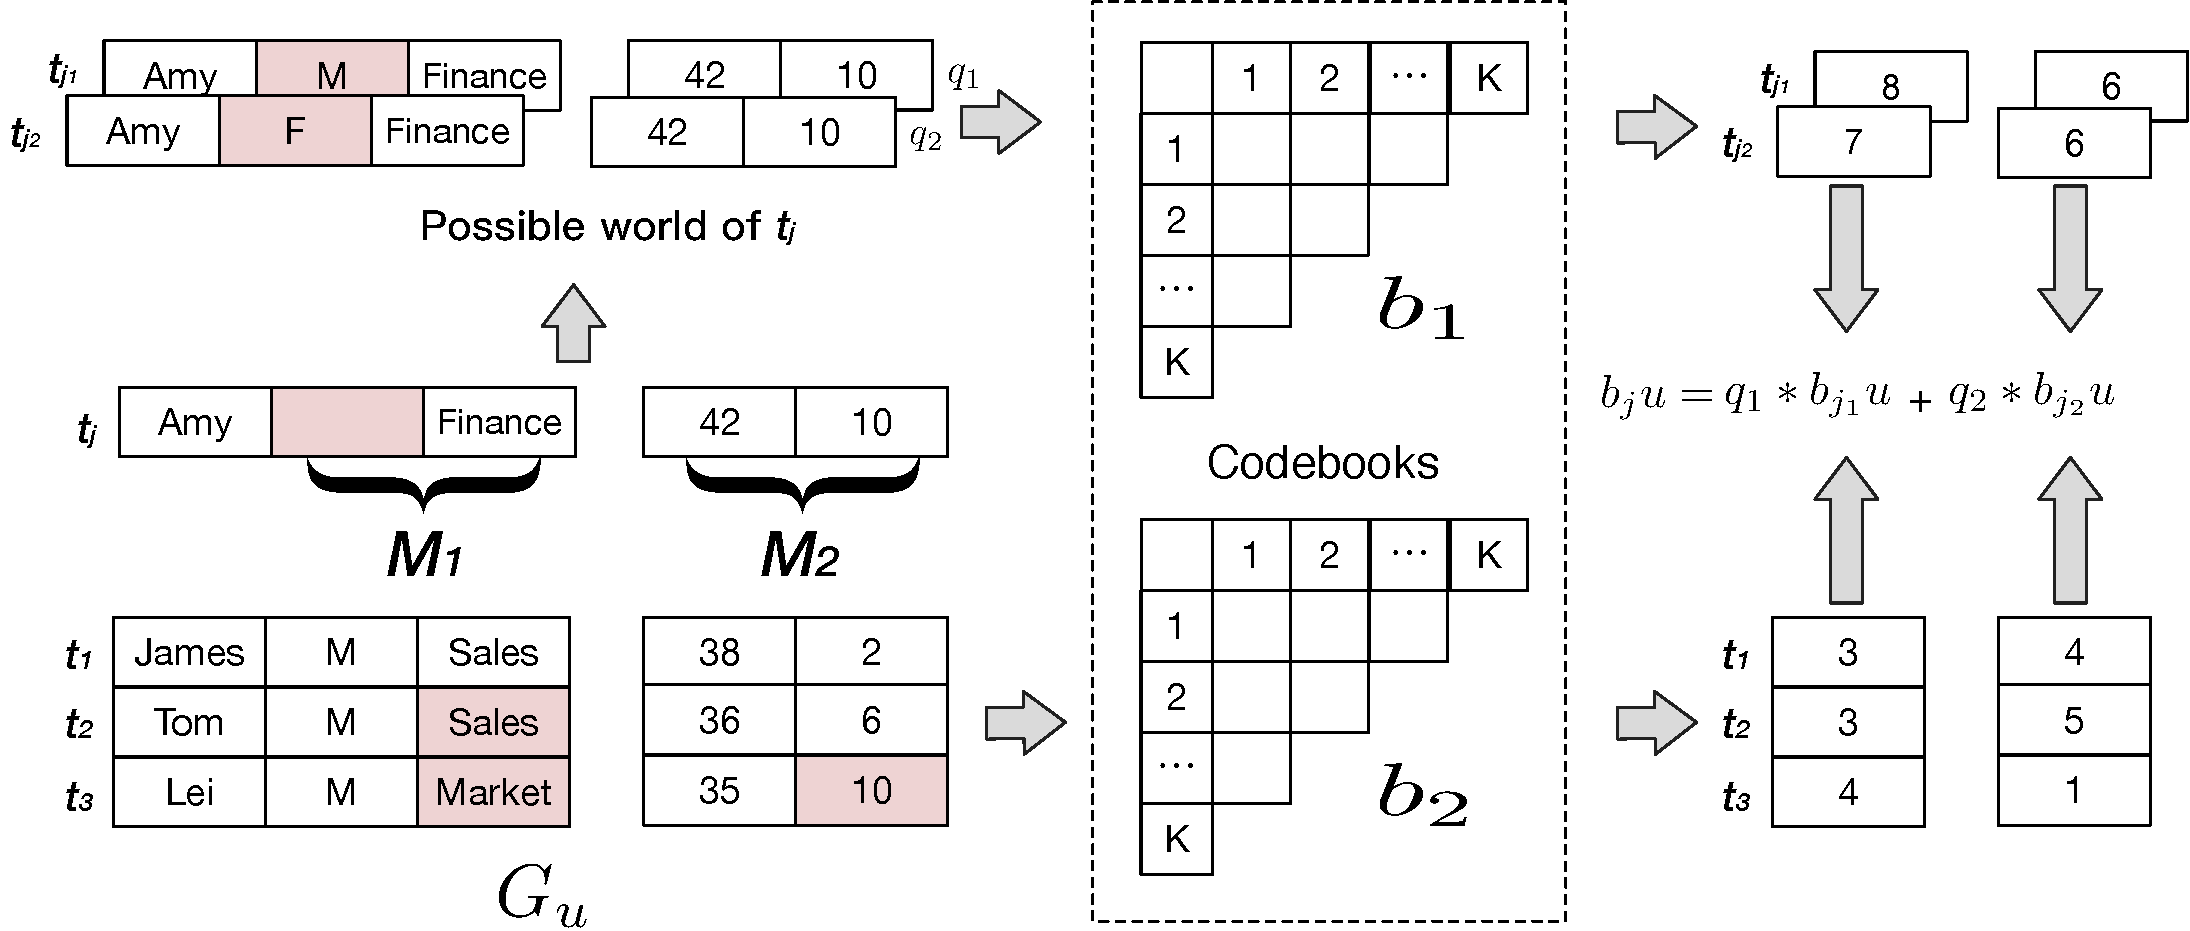
\includegraphics[width=0.6\textwidth]{figs/distance}
   % \vspace{-2.5em}
    \caption{Illustration of the Group-based Solution.}
    \label{fig:distance}
   % \vspace{-1.5em}
\end{figure}

\begin{figure}[t]
    \centering
    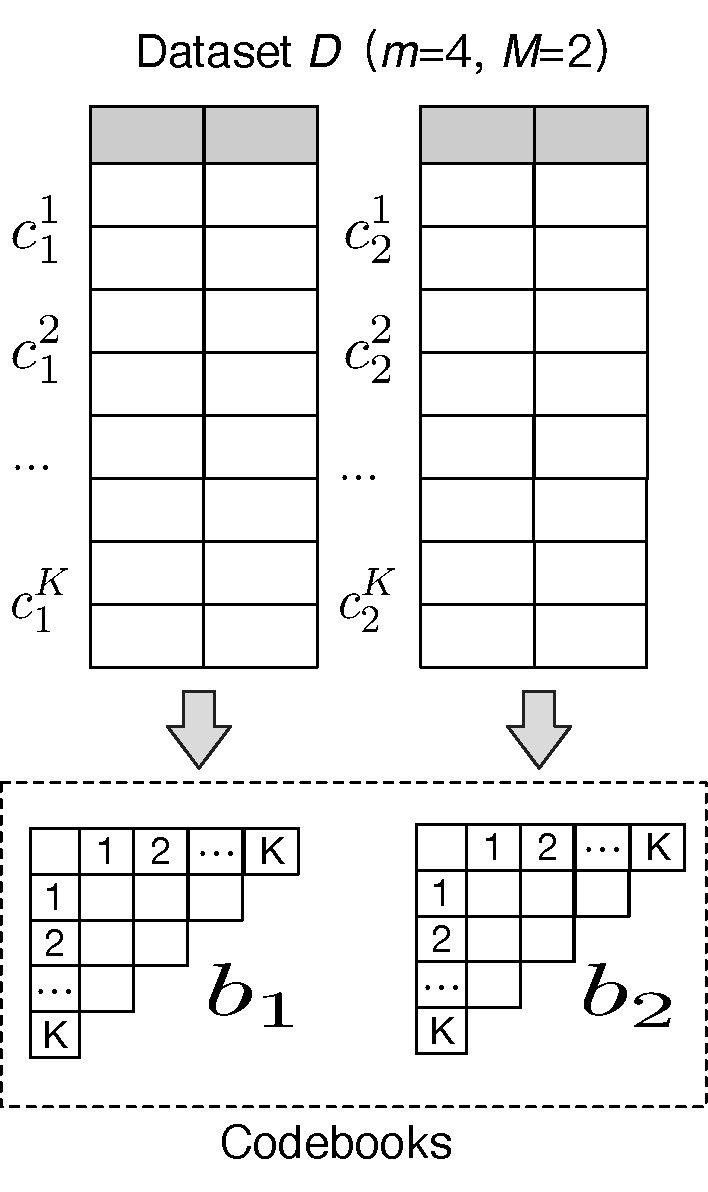
\includegraphics[width=0.6\textwidth]{figs/codebook}
   % \vspace{-2.5em}
    \caption{Illustration of the Group-based Solution.}
    \label{fig:codebook}
   % \vspace{-1.5em}
\end{figure}
%!TEX root = ../main.tex

\section{Experiment}~\label{sec:exp}

%In this section, we mainly answer the following questions: (1) How does \ours perform compared to other baselines? (2) How to implement an  end-to-end solution for \ours and how does the solution perform? (3) How does \ours perform for the batch algorithm? (4) How is the convergence of \ours ? (5) How does some parameters (\eg sample size) affect the performance of the method?

In this section, we sufficiently compare our proposed methods with multiple baselines on real datasets to demonstrate our effectiveness and efficiency. 

%!TEX root = ../main.tex
\subsection{Experimental Settings}

\noindent{\bf Dataset.} We evaluate on 6 real-world datasets that are often used in the field of data imputation~\cite{DBLP:conf/icde/LiRBZCZ21, liu2021adaptive, DBLP:journals/pvldb/KrishnanWWFG16,DBLP:journals/pvldb/KarlasLWGC0020}, as shown in Table~\ref{tbl:dataset}, where $M$ denotes the number of attributes.   
%They cover different downstream ML tasks, including binary classification, multi-classification and regression.  

%Among these datasets, there are not enough missing values in the some of them. Thus, we manually create some incomplete tuples for them. We can also obtain the ground truth of these manually created missing values to better compare different baselines. 
%In addition, numerical attribute is hard to impute, thus, we convert them to categorical attribute using bucketing technique. The details of these datasets are as below.

\noindent{\bf (1) \nursery}~\cite{nursery} is a multi-classification task, which  predicts ``{\it the level of recommendation for whether a child goes to school}''. There are five different levels, \ie $\{ {\tt not\_recom, priority, recommend, spec\_prior, very\_recom} \}$. %There are 9 categorical attributes. %The size of train, validation and test are 10960, 1000 and 1000. We manually created 3000 incomplete tuples in the train dataset.
{\bf (2) \hr}~\cite{chai2022selective} is a binary classification task of ``{\it predicting whether an employee would change the job}''.  %There are 12 attributes, one of which  is numerical. %and we convert it to categorical attribute using bucketing technique. The size of train, validation and test data are 18287, 2000 and 2000. In the train dataset, there are 5000 incomplete tuples.
{\bf (3) \adult}~\cite{adult} is a binary classification task that predicts ``{\it if the annual revenue of a people is over 50000 dollars}''. %There are 14 attributes in this dataset, 6 of which are categorical. %The size of train, validation and test dataset are 32842, 8000 and 8000. In the train dataset, there are 12500 incomplete tuples. 
{\bf (4) \credit}~\cite{kaggle} is a binary classification task that predicts ``{\it whether the loan will be deferred based on a person's economic situation}''.  %The size of train, validation and test dataset are 131,000, 4000 and 4000. In the train dataset, there are 87000 incomplete tuples.
{\bf (5) \bike}~\cite{bike} is a regression task that predicts ``{\it the number of bike sharing in a given time}''. %There are 15 attributes in this dataset, 5 of which are numerical data. %The size of train, validation and test dataset are 13300, 2000 and 2000. In the train dataset, there are 5100 incomplete tuples.
{\bf (6) \air}~\cite{auctus} is a regression task that predicts ``{\it the air quality at a certain time}''. %There are 18 attributes in this dataset, 12 of which are numerical data.
{\bf (7) \imdb}~\cite{DBLP:journals/pvldb/LeisGMBK015} refers to a dataset that \textit{predicts the rating (1-10) of movies}, which contains the basic information of movies, \eg \texttt{movie\_id, title, production\_year}.
%
{\bf (8) \imdbl}~\cite{DBLP:journals/pvldb/LeisGMBK015} is the large vision of \imdb, which contains 4,000,000 records with the same attributes.

%Table~\ref{xxx} shows the statistics of these datasets.

For datasets (1)-(3) and (7)-(8), we follow existing works~\cite{DBLP:journals/jbd/KhanH20,DBLP:conf/icml/YoonJS18,DBLP:conf/mlsys/WuZIR20} to manually inject missing values until the  rate of missing tuples is 30\%, and we will vary the percentage of incomplete tuples in Section~\ref{exp:sec:sensitivity}. Datasets (4)-(6) already contain missing values. For all datasets, we randomly split them for 80\%/10\%/10\% as train/validation/test sets.






\noindent{\bf Evaluation metrics.}
We mainly evaluate the effectiveness and efficiency of \ours and  baselines. For effectiveness, we use the {\it prediction accuracy} for the classification task and use the {\it mean square error} ($MSE = \frac{\sum_{i=1}^N(y_i-\hat{y}_i)}{N}$, where $N$ denotes the size of test set) for the regression task. 

For efficiency, we focus on the machine cost (\ie the runtime of machine) as well as the human cost (the number of tuples imputed by human for human-involved methods). For datasets (1)-(3) and (7)-(8), we have the ground truth of missing tuples, so we use them to simulate the human imputation. For datasets (4)-(6), we leverage the expert to impute missing values in the coreset by looking at the top-5 values recommended by the automatic method as a reference. Note that we only involve humans when it is affordable. For baselines that require humans to impute a lot of missing tuples (\ie~\truth~and $\one$ as below), we will not apply them on datasets (4)-(6).

\noindent{\bf Baselines.} We compare \ours and \ours$^+$ with a variety of baselines.

%\noindent{\bf (1) \noclean} refers to just training on $\train$. \cc{necessary?}



%\noindent{\bf (3) \truthcore} first uses the ground truth to impute the missing values and then selects the coreset for the cleaned dataset. Similar to \truth, it only works for the datasets with manually created missing values. 

%\noindent{\bf (3) \mice} is a typical missing value imputation approach. \mice uses linear regression to estimate the missing values. \mice conducts imputation for a missing value several times and uses the average value as the final result.

%\noindent{\bf (5) \missf} is a tree-based imputation method. It recasts data imputation as a prediction task and uses random forest to predict the missing values.

%Data are imputed by regressing each variable in turn against all other variables and then predicting missing data for the dependent variable using the fitted forest.
\begin{table}
	\centering
	\caption{Statistics of datasets}
	\vspace{-1em}
	{\small
	\begin{tabular}{ccccc}
		\hline
		{\bf Dataset} & {\bf $|\train|$} & {\bf $m$} & {\bf $\#$ Incomp. Tuples} & {\bf Task}\\
		\hline	
		\nursery & 	10960 & 9 & 3218 & Multi-Class. \\
		\hr & 18287 & 12 & 5475 & Binary Class. \\
		\adult & 32842 & 14 & 10752 & Binary Class. \\
		\credit & 131,000 & 11 & 76813 & Binary Class. \\
		\bike & 13300 & 15 & 4821 & Regression \\
		\air & 437,200  & 18 & 128,372 & Regression\\
		\imdb & 1,000,000 & 40 & 331,189 & Multi-Class.\\
		\imdbl & 4,000,000 & 40 & 1,312,908 & Multi-Class.\\
		\hline
	\end{tabular}
	}
	\label{tbl:dataset}
%	\vspace{-1.8em}
\end{table}

\noindent{\bf (1) \noclean}~refers to just training on $\train$.

\noindent{\bf (2) \actclean}~\cite{DBLP:journals/pvldb/KrishnanWWFG16} is an iterative data cleaning framework, which estimates the impact of tuples  and prioritizes cleaning the tuples that much affect the model performance. In each iteration, it can ask the human to clean a sample subset of tuples. We set the sample size to 50, same as the paper. 

\noindent{\bf (3) \boostclean}~\cite{DBLP:journals/corr/abs-1711-01299} is an automatic  data cleaning method that iteratively selects a cleaning method from several pre-defined algorithms, applies to the train dataset and  updates the model.  We use MICE~\cite{royston2011multiple}, MISSForest~\cite{DBLP:journals/bioinformatics/StekhovenB12}, GAIN~\cite{DBLP:conf/icml/YoonJS18} as pre-defined algorithms.


\noindent{\bf (4) \gain}  uses MICE~\cite{royston2011multiple}, MISSForest~\cite{DBLP:journals/bioinformatics/StekhovenB12}, GAIN~\cite{DBLP:conf/icml/YoonJS18} to respectively impute the train set and selects the one that achieves the highest accuracy on the validation set.

\noindent{\bf (5) \truth} is an ideal case that trains on the ground truth, \ie $\trainc$. Note that only datasets (1)-(3) have the ground truth to evaluate this baseline.  Datasets (4)-(6) do not have the ground truth and it is  too expensive to ask the human to impute so many missing values.

\noindent{\bf (6) \mixcore} is a baseline that selects a coreset from all complete tuples, and then we randomly select some incomplete tuples to impute. We set the number of incomplete tuples to be imputed equal to that of  other baselines for fair comparison. Finally we train with the tuples in the coreset plus the  imputed ones.



%It treats the data cleaning as a minimax optimization problem. The generator is optimized to impute the incomplete tuples and makes them as similar as possible to the complete tuples. While the discriminator is utilized to distinguish the imputed tuples. Thus, the incomplete tuples can be imputed during this minimax game.

%\noindent{\bf (7) \rand} randomly samples a subset from the dirty dataset $\train$ and imputes the missing values in it. Then, it trains a downstream model on this subset.


\noindent{\bf (7) $\one$} first involves human to impute the dataset $\train$ and then selects a coreset. Similar to \truth, only datasets (1)-(3) can be evaluated on it because they have the ground truth. The coreset selection solution is the algorithm in~\cite{DBLP:conf/icml/MirzasoleimanBL20}, which is a greedy algorithm by modifying Algorithm 1 without considering the possible worlds.


\noindent{\bf (8)  $\two$} first uses automatic data imputation methods to impute the dataset $\train$, and then selects a coreset using the same method of baseline (7).

\noindent{\bf (9) $\three$} directly selects a coreset based on $\train$ and then asks human to impute the incomplete tuples of the coreset.

\noindent{\bf (10) $\four$} also directly selects a coreset from $\train$, it then uses MICE~\cite{royston2011multiple} to impute the incomplete tuples in the coreset.

\noindent{\bf Our solutions.} We compare \ours and its variants.

\noindent{\bf (11) $\seven$} uses \ours to select the coreset and iteratively asks human to impute incomplete tuples (one tuple per human iteration) during the coreset selection process.

\noindent{\bf (12) $\eight$} is similar to $\goodfunc(\train,\circlearrowleft^\humanfunc)$, but the automatic  MICE  method is used.

\noindent{\bf (13) $\nine$} uses group-based method to accelerate \ours, which selects the coreset and iteratively asks human to impute incomplete tuples (one tuple per human iteration) during the coreset selection process.

\noindent{\bf (14) $\ten$} is similar to $\nine$, but the automatic  MICE  method is used.


Besides, since the coreset of $\five$ (or $\six$) is too expensive to compute due to the large number of possible worlds, we do not directly compare with it. Instead, we will limit the number of possible worlds of each tuple to 3 as discussed in Section~\ref{subsec:batch} and evaluate in Section~\ref{exp:sec:batchalgo}.

%\noindent{\bf (12) $\five$} first uses \ours to select a coreset and then involves human to impute this coreset. Since the machine cost is too high, we limit the number of possible worlds of each tuple to 3 and evaluate in Section~\ref{exp:sec:batchalgo}.

%\noindent{\bf (13) $\six$} also uses \ours to select a coreset and leverages MICE to impute this coreset. For the same reason as $\five$, we also  limit $l=3$  and evaluate in Section~\ref{exp:sec:batchalgo}.

 



%\noindent{\bf (10) \autocore} first uses an automatic data imputation method (\eg MICE) to impute the dirty dataset $\train$. Then, it selects a coreset of the cleaned dataset and involves human to review the missing values in the coreset.




\noindent{\bf Hyper-parameter setting.}
%For classification tasks, we use SVM as the default downstream model. For regression tasks, we use linear regression as the default.
We use SVM and linear regression as the default downstream model for classification and regression tasks, respectively. We vary the downstream models in Section~\ref{exp:sec:sensitivity}. For model training, we use SGD and k-inverse decay  scheduling, \ie $\alpha_k = \alpha_0 / (1+bk)$ ($\alpha_0$ and $b$ are hyper-parameters to be tuned independently for different methods).  The sample size $h$ is set to 200 as default and we vary the  size in Section~\ref{exp:sec:sensitivity}. The number of training epochs is set as 20. %\cc{
We also impute the test data using the same method that is applied to the train data before testing.
%}

%!TEX root = ../main.tex



\subsection{Overall Evaluation}\label{exp:sec:overall}

\begin{table}
	\centering
	\caption{Human cost of different methods}
	\vspace{-1.2em}
	\small
	\begin{tabular}{ccccc}
		\hline
		Dataset & $\nine$ & $\seven$ & $\three$ & $\one$\\
		\hline
		\nursery & 35 & 37 & 22 & 3278\\
		\hr & 48 & 44 & 32 & 5475\\
		\adult & 60 & 63 & 81 & 10752\\
		\credit & 57 & 52 & 67 & -\\
		\bike & 35 & 38 & 25 & -\\
		\air & 100 & 98 & 102 & -\\
		\imdb & 215 & 220 & 230 & 331189\\
		\imdbl & 520 & 511 & 530 & 1312908 \\
		\hline
	\end{tabular}
	\label{tbl:humancost}
	\vspace{-1em}
\end{table}





In this part, we compare \ours \jks{and \ours$^+$} solutions with baselines. We use $\rho = \frac{K}{|\train|}$ to denote the proportion of coreset  to the entire train set.  %\cc{
We set  $\rho=0.005$ for datasets (1)-(4), $\rho=0.001$ for datasets (5) and  $\rho=0.0005$ for larger datasets (6)-(8).
%}
 We  will further  conduct evaluation by varying the coreset size  in Section~\ref{exp:sec:end2end}.




\subsubsection{Evaluation of model accuracy.}
The results are provided in Figure~\ref{fig:effectiveness_old} \jks{and Figure~\ref{fig:effectiveness_new}}. To summarize, the result could be generally ranked as $\seven/\one/\truth$ >  $\eight/\boostclean/\gain$ > $\two$ > $\mixcore$ > $\actclean$ > $\three/\four$ > $\noclean$.
Next, we explain the results.

In general, on all datasets, our method $\seven$, \truth~ and $\one$~   perform the best. 
 \truth~ and $\one$ achieve a high accuracy because they ask the human to impute missing values accurately, but incur a high human cost.  For example, \truth~and $\one$ achieve accuracy of 71.9\% and 71.7\% on \adult. $\seven$  is competitive with them because it selects a good coreset that can well represent the unknown ground truth via gradient approximation. In addition, we can observe that $\seven$ performs better than $\eight$ because human imputation is more accurate than automatic methods. For example, on \adult, $\seven$ has an accuracy of 71.7\%, while $\eight$ and others are below 68\%. $\eight$, \boostclean and \gain have competitive performance on accuracy. \boostclean and \gain can have a not bad performance because they impute all tuples and train on the entire dataset, but they cannot achieve efficient training (see \ref{sec:exp:efficiency}). But  we can train on the much smaller coreset generated by $\eight$ with a good accuracy, because \ours considers the possible repairs to derive the coreset  that can approximate the full gradient of the entire dataset. Given the same number of tuples to be imputed by human,  $\seven$ also outperforms \actclean because we have theoretical guarantees on the gradient approximation. 
 %For example, on dataset \adult, $\eight$ has an accuracy of 69.8\%, which is better than that of \boostclean (65.8\%), \actclean (63.9\%) and \gain (65.1\%). Our method $\eight$ outperforms \boostclean because we consider possible repairs and the gradients of tuples in our algorithm.   \actclean also considers gradients of tuples, which prioritizes imputing tuples that much influence the model gradients, but they use heuristics to estimate the influence, which is not accurate enough. \gain does not perform well because it does not much consider possible repairs and not impute the tuple considering the downstream model performance.
  For other baselines,  $\three$ and $\four$ do not perform well because they select the coreset from an incomplete dataset.  $\two$ cannot achieve a good performance because the selected coreset can not well represent the complete entire dataset, as it does not consider possible repairs as our method.  %it is hard for the automatic method to always achieve a high imputation accuracy. 
  {\mixcore} does not perform well (\eg 65.2\% on \adult) because $\seven$ and $\eight$ select a better coreset considering the full data. For \noclean, on  \adult, the model  has an accuracy of 61.3\% because of the incomplete tuples.



 



\subsubsection{Evaluation of the efficiency.}~\label{sec:exp:efficiency} We  evaluate the efficiency of all methods, including the machine cost and human cost.

\noindent{\bf Machine cost.} Machine cost is shown  in Figure~\ref{fig:efficiency_old}.  The results could be ranked as $\three/\four/\seven/\eight/\one/\mixcore < \two < \truth < \noclean < \actclean < \boostclean/\gain$. We can observe that the first 5 methods in the ranking have low machine cost, mainly because they train based on the selected coreset and do not need iterative training. $\seven$ and  $\eight$ are slightly slower  because they need to iterate several possible repairs during the process of coreset selection.  But $\seven$ is still more efficient than \noclean, \truth, \boostclean and \gain by more than one order of magnitude,  because they need to train on the entire training data. 
 Moreover, \actclean~  and \boostclean are  not efficient either because they incorporate multiple training times, so as to estimate the gradient while data imputation. \gain is slow because training multiple imputation models takes time.


\noindent{\bf Human cost.} In terms of the human cost, $\one$, $\three$, $\seven$ and  \actclean~ involve human. As shown in~Table~\ref{tbl:humancost}, $\one$ is very expensive because it asks the human to impute all missing tuples. For example, on datset \adult, 10752 tuples have to be imputed. We do not compare \credit, \bike and \air for $\one$ because they do not have the ground truth.
 But $\three$ and $\seven$ are cost-effective because human just needs to impute missing tuples in the much smaller coreset. For example, they only cost 81 and 63 tuples on dataset \adult respectively. 
\actclean~ asks the human to iteratively impute the data. Given the same number of tuples to impute, our method can achieve much higher accuracy. We will  evaluate it in details in next subsection.
 



\noindent \textbf{Summary.} 
Based on the results, we have the following conclusions.
(1) Our proposed methods $\seven$ and $\eight$ can achieve high model accuracy because the selected coreset can well represent the underlying ground truth by gradient approximation considering possible repairs. Meanwhile, they are practical because of the low machine cost. (2) Compared with $\one$ that involves human to impute the entire dataset $D$, the human cost of $\seven$ is much lower, as observed in Table~\ref{tbl:humancost}, e.g., $37$ vs. $3278$ on the \nursery dataset. Thus, we can choose $\seven$ when we want to achieve high model accuracy and afford a certain human cost. (3) 
%Meanwhile, they are practical because of the low machine cost. Although $\seven$ needs human involvement, the human cost is also low. We can choose it when we want to achieve high model accuracy. 
If we neither care very much about the accuracy nor consider to incur human cost, the much more efficient $\eight$ is a good choice.

%!TEX root = ../main.tex
\subsection{Evalution of \texttt{GoodCore}$^+$}
\label{exp:sec:G+}

In this part, we evaluate the efficacy of  \texttt{GoodCore}$^+$. 

\begin{figure*}
	\centering
	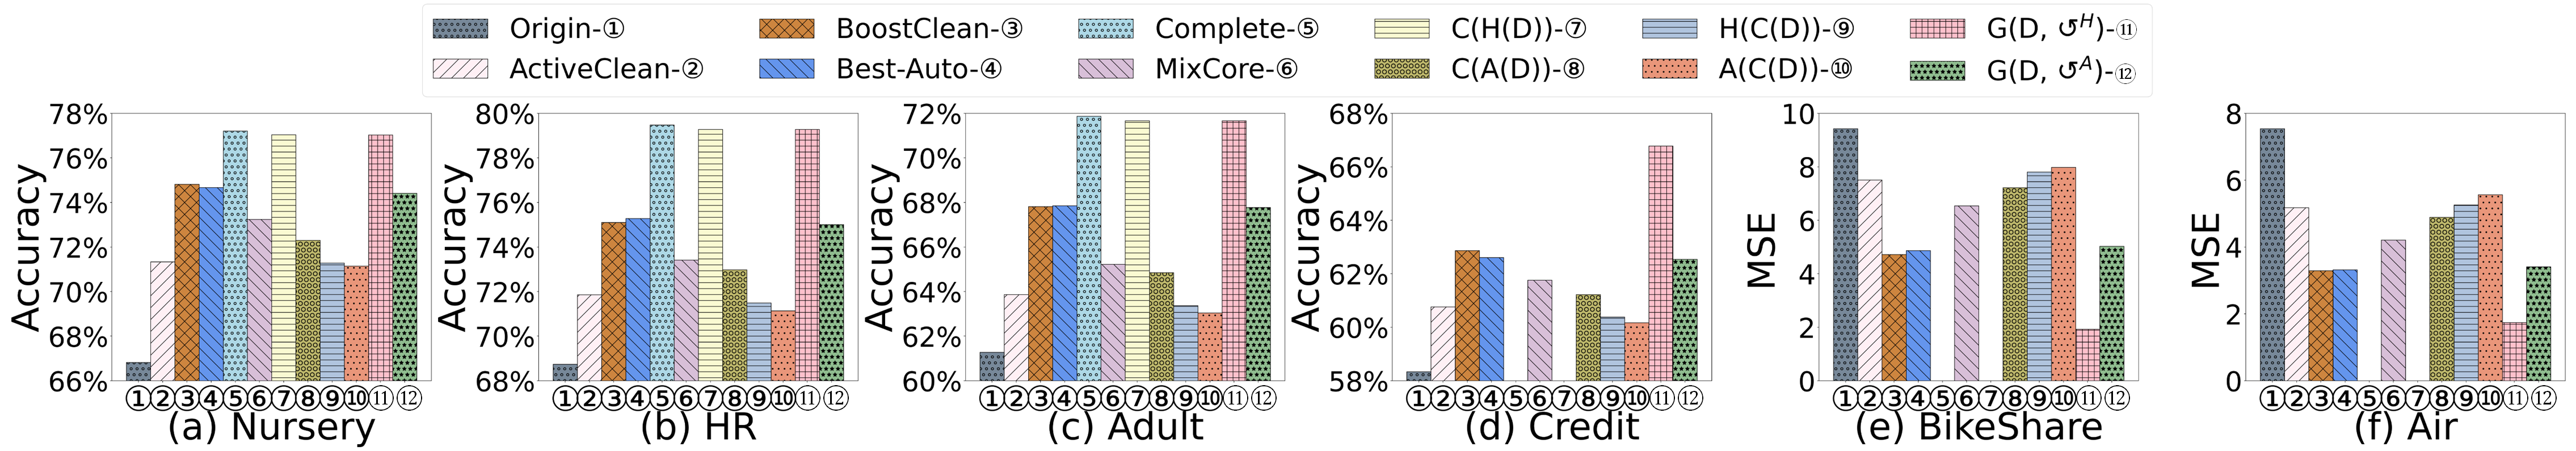
\includegraphics[width=\textwidth]{figs/effectiveness_new}
%	\vspace{-2.5em}
	\caption{Effectiveness of $G$ vs $G^+$.}
	\label{fig:effectiveness_new}
%	\vspace*{-1.2em}
\end{figure*}

\begin{figure*}
	\centering
	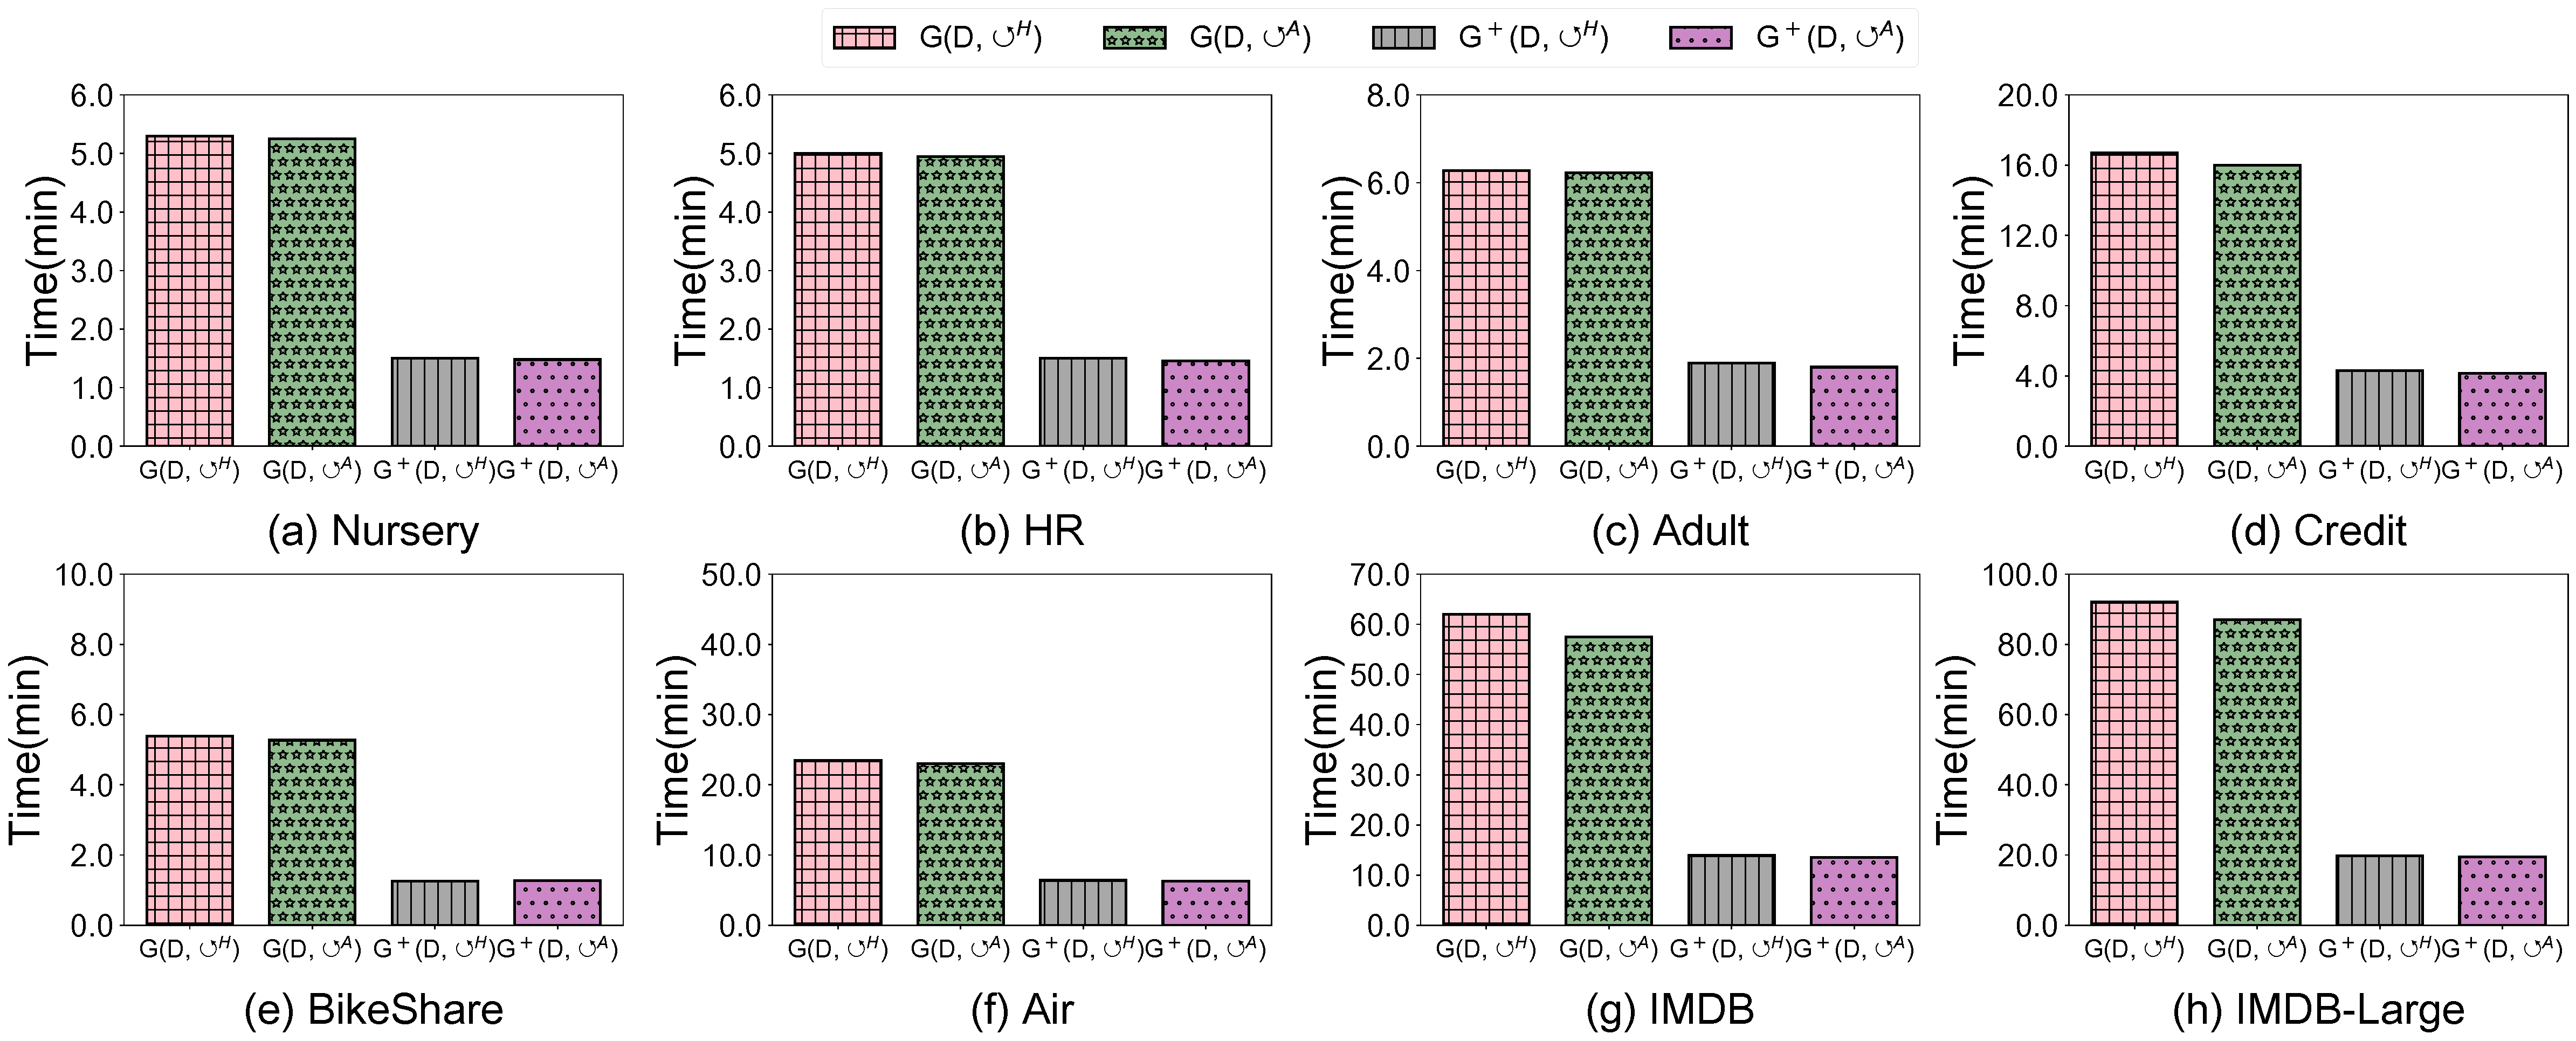
\includegraphics[width=\textwidth]{figs/efficiency_new}
%	\vspace{-2.5em}
	\caption{Efficiency of $G$ vs $G^+$. Note that only machine cost (i.e., runtime of machine) is considered.}
	\label{fig:efficiency_new}
%	\vspace*{-1.5em}
\end{figure*}

\subsubsection{Evaluation of model accuracy.}
The results are provided in Figure~\ref{fig:effectiveness_new}. We can found that the accuracy of \texttt{GoodCore}$^+$ and \ours are roughly the same on all datasets. For example, on dataset \imdbl,  $\nine$and $\seven$ achieve accuracy of 74.7\% and 74.9\% and they differ from each other by 0.2\%. This is because both of them   select a good coreset because of a bounded GA error. In addition, we can observe that $\nine$ performs better than $\ten$ because human imputation is more accurate than automatic methods. For example, on \imdbl,  $\nine$ has an accuracy of 74.7\%, higher than that of $\eight$.

\subsubsection{Evaluation of the efficiency.}~\label{sec:exp:efficiency_g} We  evaluate the efficiency of \texttt{GoodCore}$^+$ and \ours, including the machine cost and human cost.

\noindent{\bf Machine cost.} Machine cost is shown  in Figure~\ref{fig:efficiency_new}.  \texttt{GoodCore}$^+$ is more efficient than \ours. For example, on \imdbl, $\nine$ spends about 12min, which is $4.8\times$ faster than $\seven$. That is because $\nine$ have the lower time complexity than $\seven$, which is discussed in Section~\ref{subsec:pq}.


\noindent{\bf Human cost.} In terms of the human cost, as shown in~Table~\ref{tbl:humancost}, $\nine$ and $\seven$ are cost-effective because humans just need to impute missing tuples in the much smaller coreset. For example, they only cost 520 and 511 tuples on dataset \imdbl respectively. 

\noindent \textbf{Summary.} 
Based on the results, we have the following conclusions. (1) Although we group tuples over the entire train set, our proposed methods $\nine$ and $\ten$ still achieve high  accuracy because the gradient approximation error can still be bounded. (2) The efficiency is much improved compared with \ours because we just need to iterate these groups rather than  the entire train set within the 3-loop coreset selection process. (3) The human cost is competitive with $\seven$ because the group-based solution has low impact on the number of tuples to be imputed by humans.

%(1) Our proposed methods $\nine$ and $\ten$ achieve high model accuracy due to the carefully selected coreset, which effectively represents the underlying ground truth through gradient approximation while considering potential repairs. Additionally, their practicality is evident through their low machine cost. (2) In comparison to $\seven$, the human cost associated with $\nine$ is significantly reduced, as demonstrated in Fig~\ref{fig:efficiency_new}, such as $11.9$min versus $57$min on the \imdbl dataset. Therefore, opting for $\nine$ is advisable when aiming for high model accuracy while managing a specific level of human cost. (3) Conversely, if neither accuracy nor human cost is a primary concern, the notably more efficient $\ten$ presents itself as an appealing option.


%!TEX root = ../main.tex
\vspace{-0.5em}
\subsection{Coreset Size Selection of \ours}
\label{exp:sec:end2end}

% \begin{figure}
% 	\centering
% 	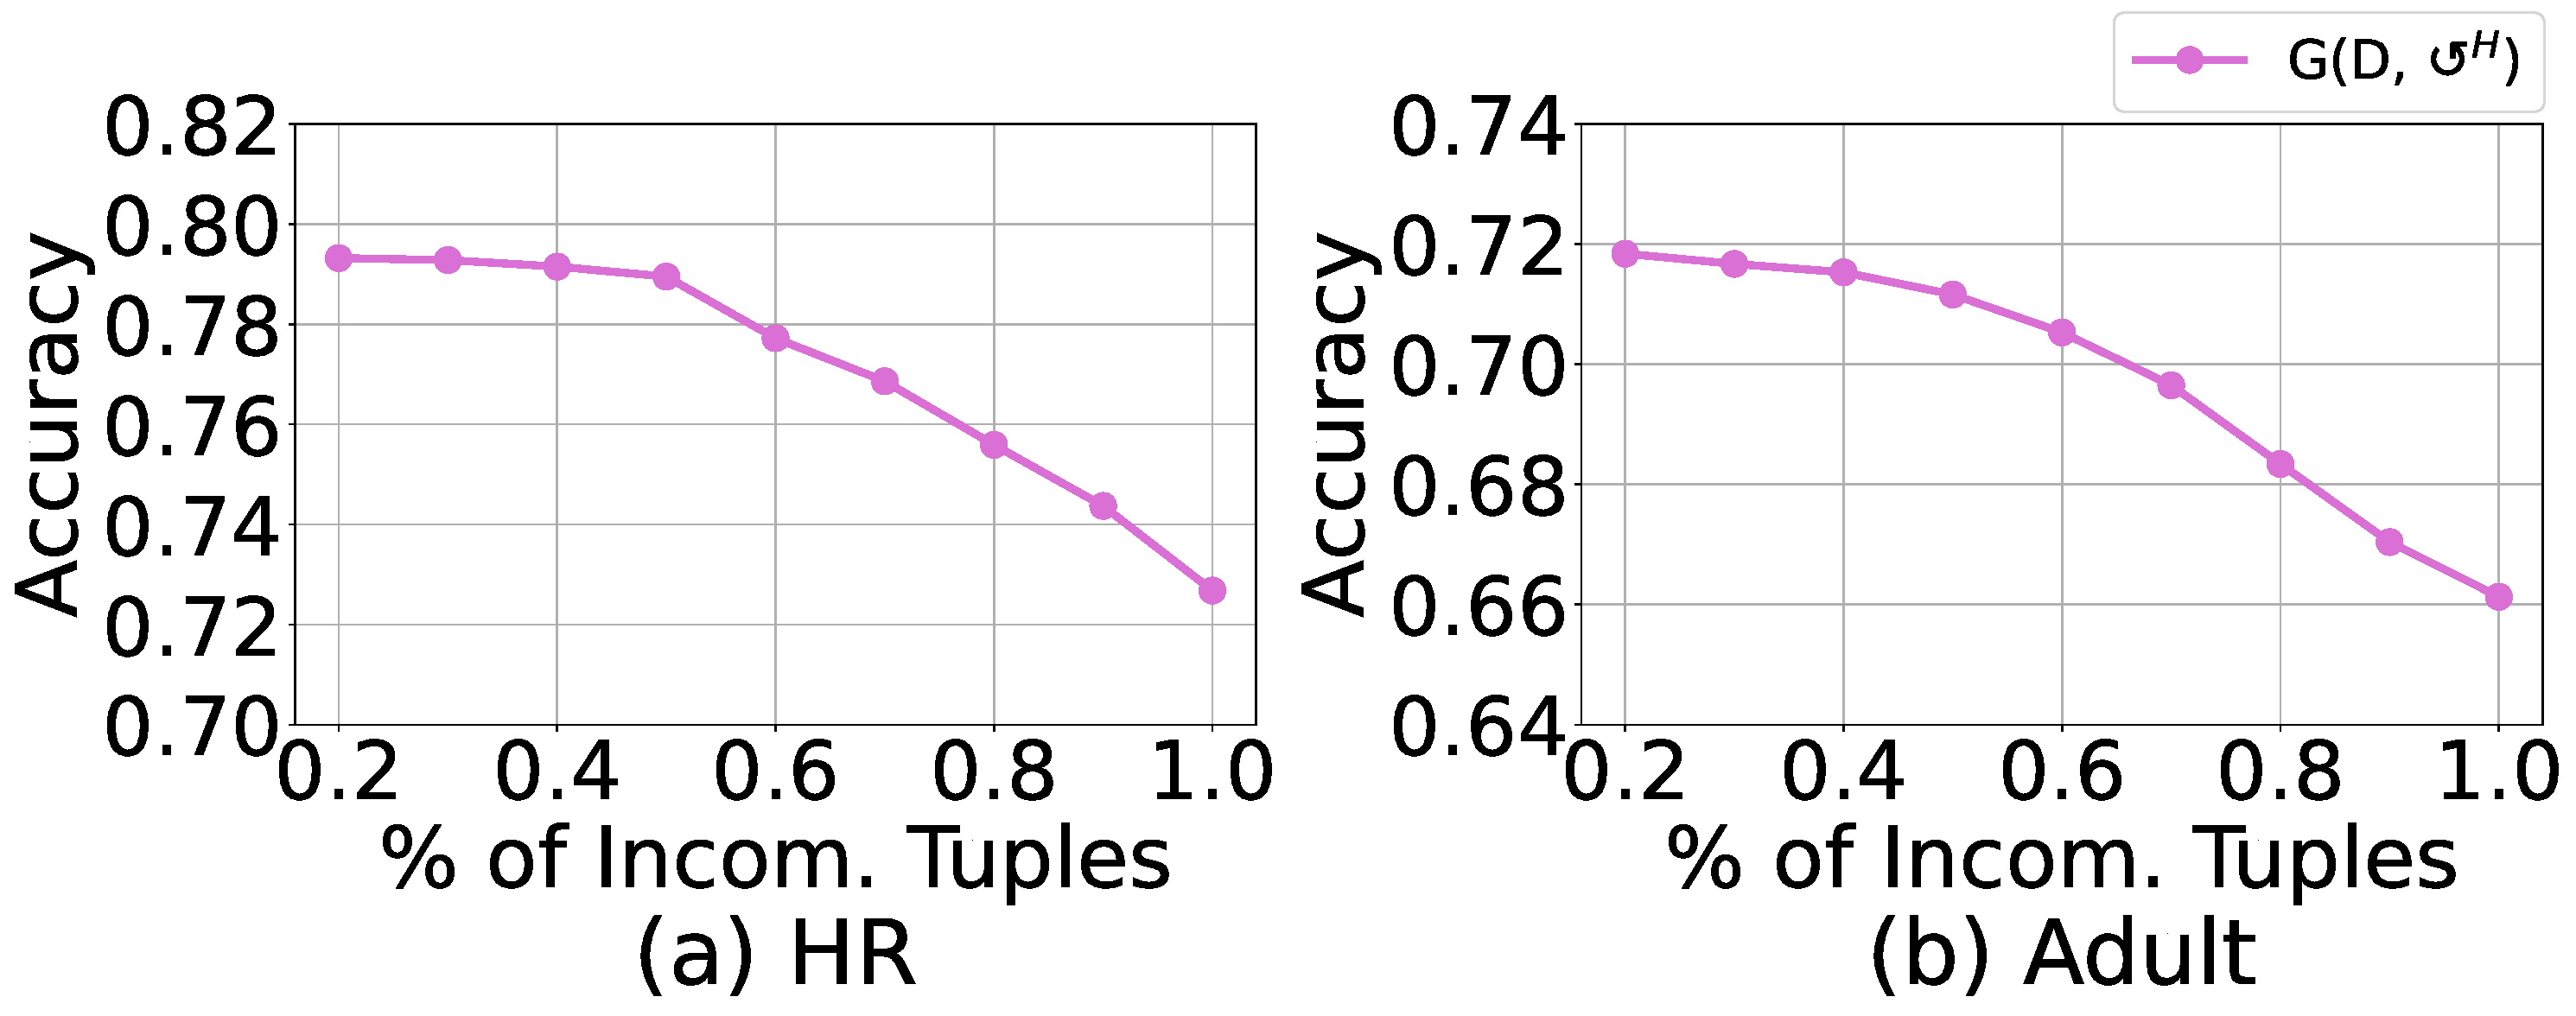
\includegraphics[width=0.5\textwidth]{figs/missingrate_all}
% %	\vspace{-1em}
% 	\caption{Varying missing tuple rate.}
% 	\label{fig:vary_misstuple_all}
% %	\vspace{-1em}
% \end{figure}

% \begin{figure}
% 	\centering
% 	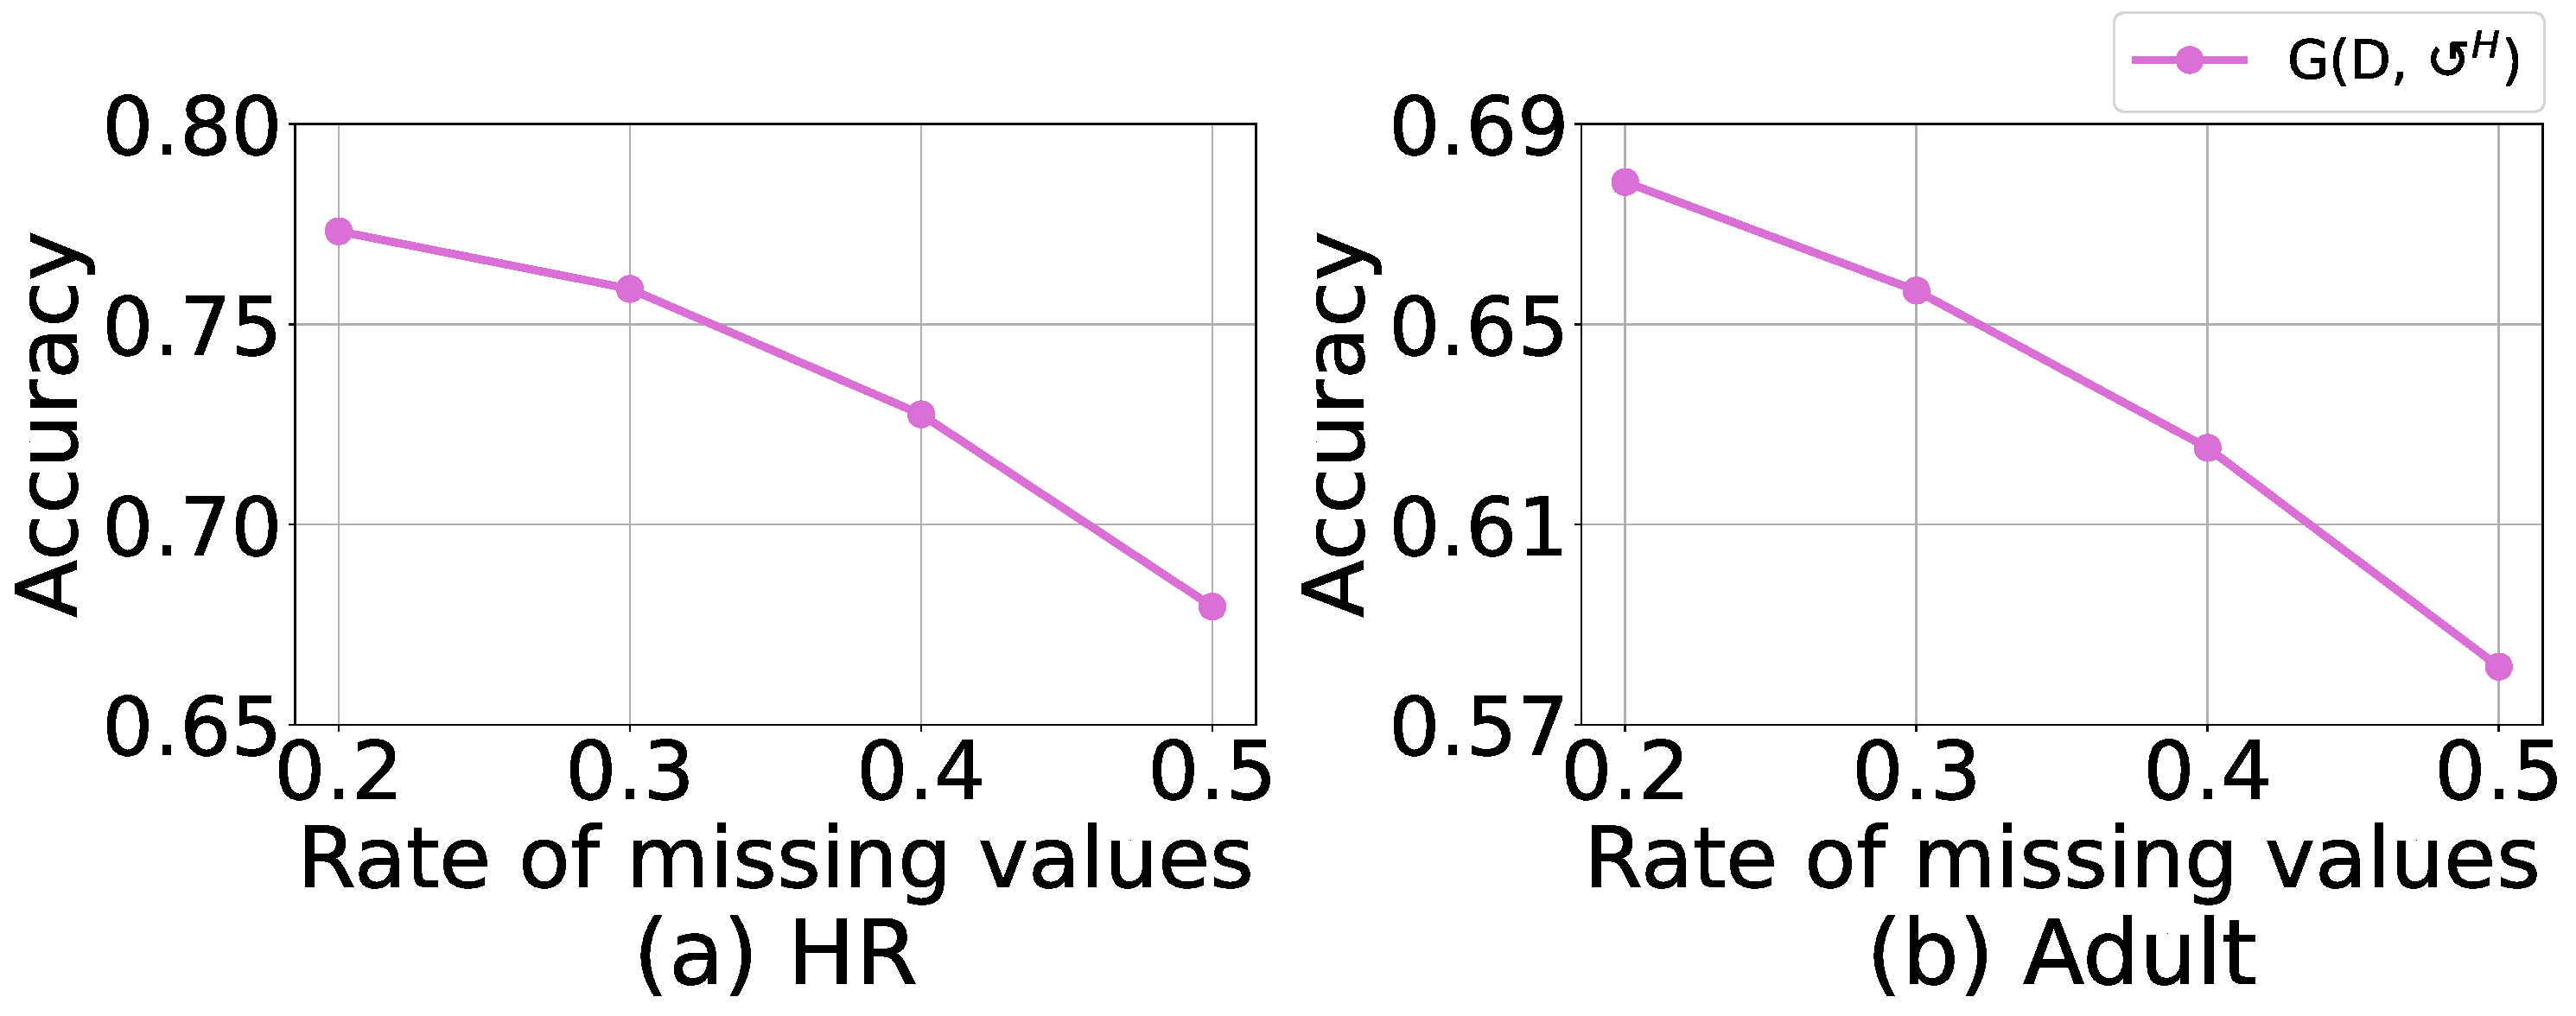
\includegraphics[width=0.5\textwidth]{figs/missingrate_real}
% %	\vspace{-1em}
% 	\caption{Varying missing value rate.}
% 	\label{fig:realmissrate}
% %	\vspace{-1em}
% \end{figure}

Recap that \ours needs the user-specified coreset size as input. Thus, we discuss how to select an appropriate coreset size. We adopt a simple yet effective solution that starts from a coreset with a small size, train over it and
evaluate via a validation set, enlarge the coreset and iteratively
train  until the performance does not improve much. 
To be specific, initially, we begin with $\rho = 10^{-4}$, and   enlarge the coreset by 2 times iteratively. If the performance on validation set varies no more than 0.5\% within three
successive iterations, we will
stop.
 Figure~\ref{fig:e2e} shows the performance on dataset \hr, \adult and \bike when varying the coreset size. We can see that the performance first improves rapidly, then remains  stable just after several iterations. For example, on dataset \adult, when $\rho=5\times 10^{-3}$, the accuracy has improved  to 72.85\% on the validation set. Empirically, an ideal coreset size is between $\rho=10^{-3}$ to $10^{-2}$.

 \begin{figure}
	\vspace{-1em}
	\centering
	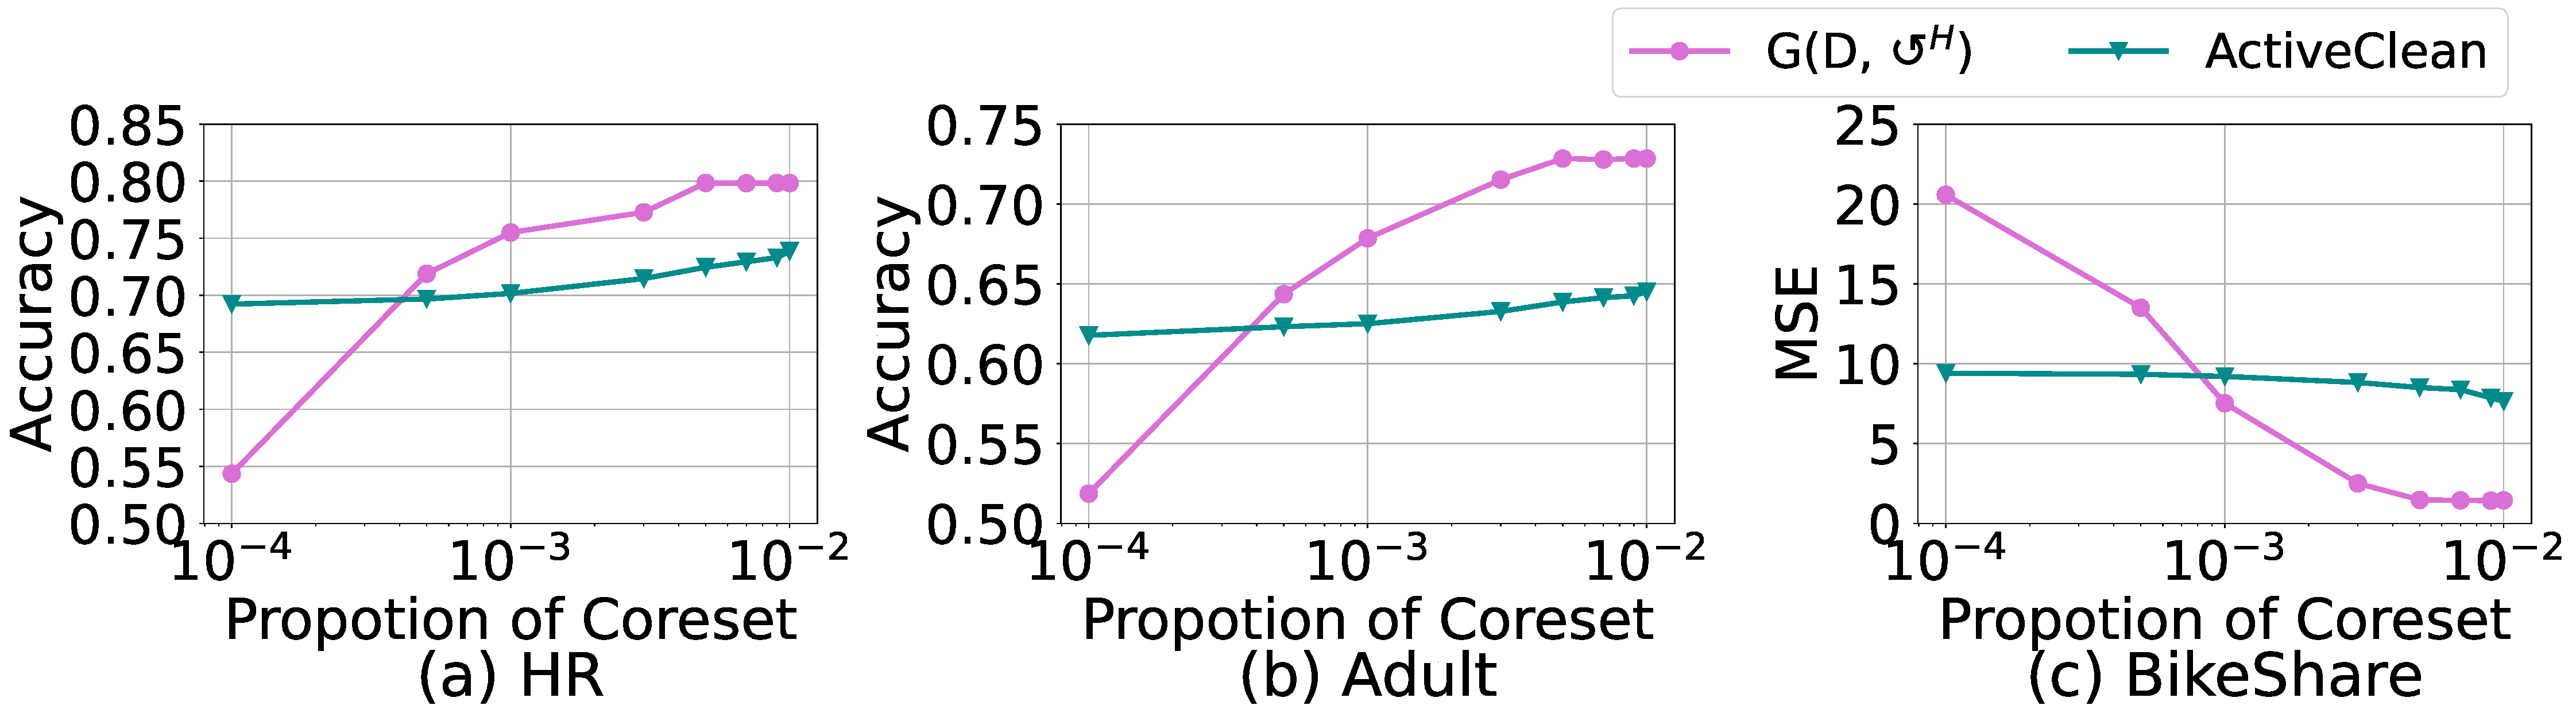
\includegraphics[width=0.8\textwidth]{figs/e2e}
%	\vspace{-2.5em}
	\caption{ Coreset size selection of \ours.}
	\label{fig:e2e}
%	\vspace{-1.8em}
\end{figure}
 
\noindent \textbf{Summary.} The results show that coreset size is not difficult to determine. If the user is willing to specify a coreset size like in Section~\ref{exp:sec:overall} based on the empirical finding, we can directly compute a coreset without training. If she cannot, we can also get a good coreset with just several training iterations over small coresets, which is also efficient.
 
\begin{figure}   
	\centering
	\begin{minipage}[t]{0.49\textwidth}
		\centering
		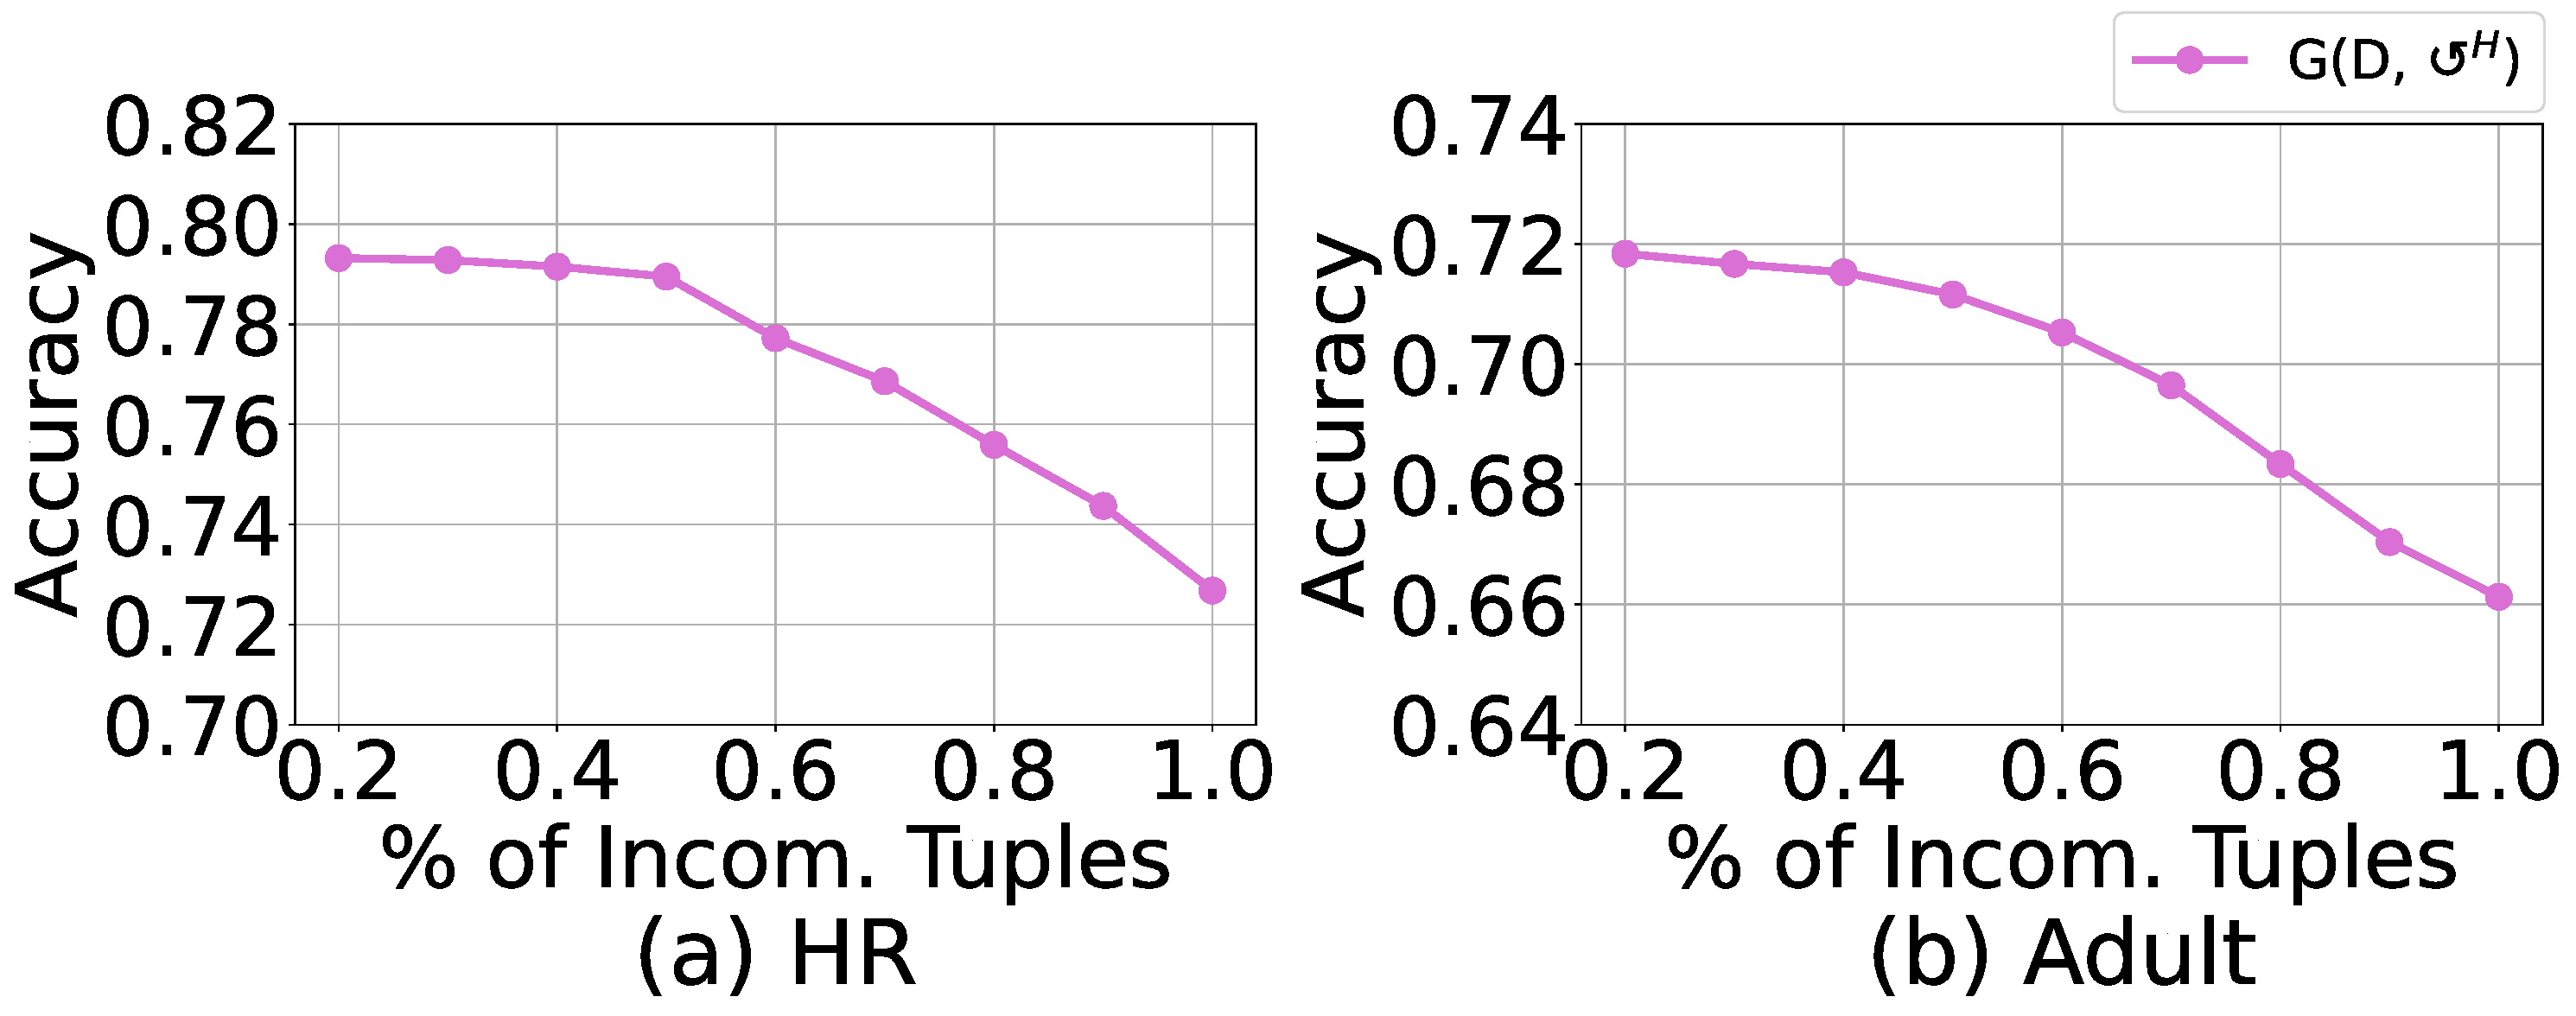
\includegraphics[width=\textwidth]{figs/missingrate_all}
    %	\vspace{-1em}
        \caption{Varying missing tuple rate.}
        \label{fig:vary_misstuple_all}
	\end{minipage}
	\begin{minipage}[t]{0.49\textwidth}
		\centering
		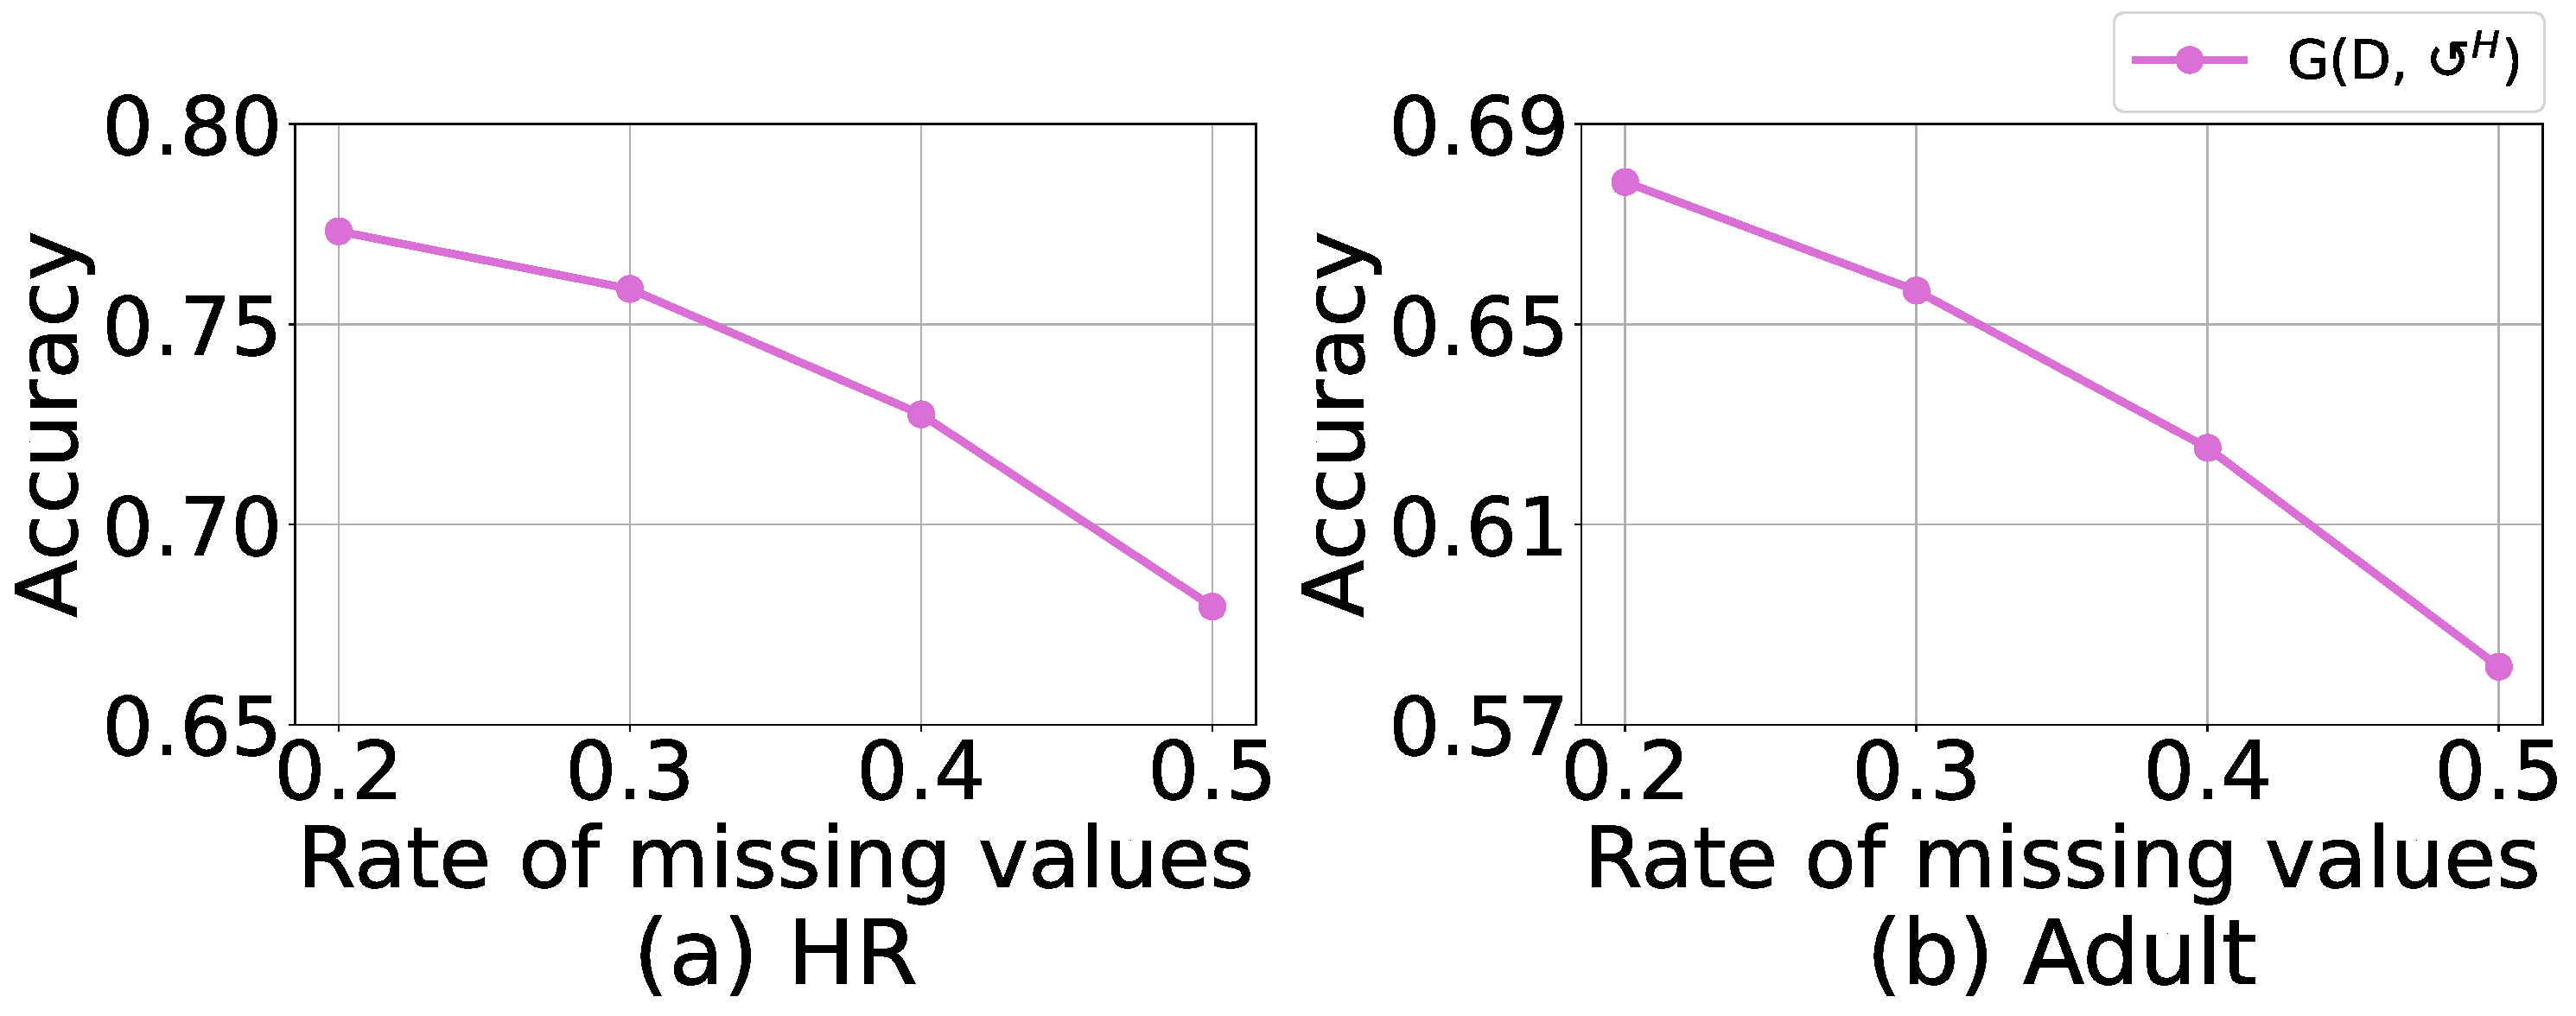
\includegraphics[width=\textwidth]{figs/missingrate_real}
    %	\vspace{-1em}
        \caption{Varying missing value rate.}
        \label{fig:realmissrate}
	\end{minipage}  
\end{figure}

\noindent{\bf Compare with \actclean.} 
Figure~\ref{fig:e2e} also reports an interesting comparison with \actclean. Specifically, 
in \actclean, we use the coreset size $K$ as the budget, i.e., number of tuples to be imputed by human in each active cleaning iteration.  
We can observe that at the beginning, when the coreset size is very small, \actclean is better because it trains with the entire dataset including the imputed tuples, while we train the model using only  few tuples in the coreset.
However, as with the increase of the coreset size, we can see that $\seven$ outperforms \actclean. This is because \actclean uses a heuristic method to estimate the impact of tuples to the overall gradient, which is not theoretically bounded (e.g., with gradient bounds like Coreset) and thus not accurate enough.
For $\seven$, it can achieve high accuracy with a proper coreset size, which is not large.











 


%!TEX root = ../main.tex

\subsection{Batch Algorithm of \ours}
\label{exp:sec:batchalgo}

In Section~\ref{exp:sec:overall} \jks{and Section~\ref{exp:sec:G+},}, $\seven$ \jks{and $\nine$} outperform other baselines on accuracy, but require many human iterations. In this part, we evaluate  the batch algorithm of \ours and \ours$^+ji$ by varying the batch size $b$, \ie Algorithm~\ref{alg:batch} to reduce the number of iterations. Intuitively, the algorithm is  $\seven$  when $b=1$. 
Then we increase $b$ until a single batch with a size $b$ can contain all incomplete tuples in the coreset with size $K$, which is in fact the algorithm $\five$.
 Due to the large number of possible worlds, we adopt the heuristic method in Section~\ref{subsec:batch} to set $l=3$ when $b>1$ \jks{for \ours and we set $l=3$ and $l_G=3$ for \ours$^+$ according to Section~\ref{subsec:pq}}. 

 \begin{figure}   
	\centering
	\begin{minipage}[t]{0.32\textwidth}
		\centering
		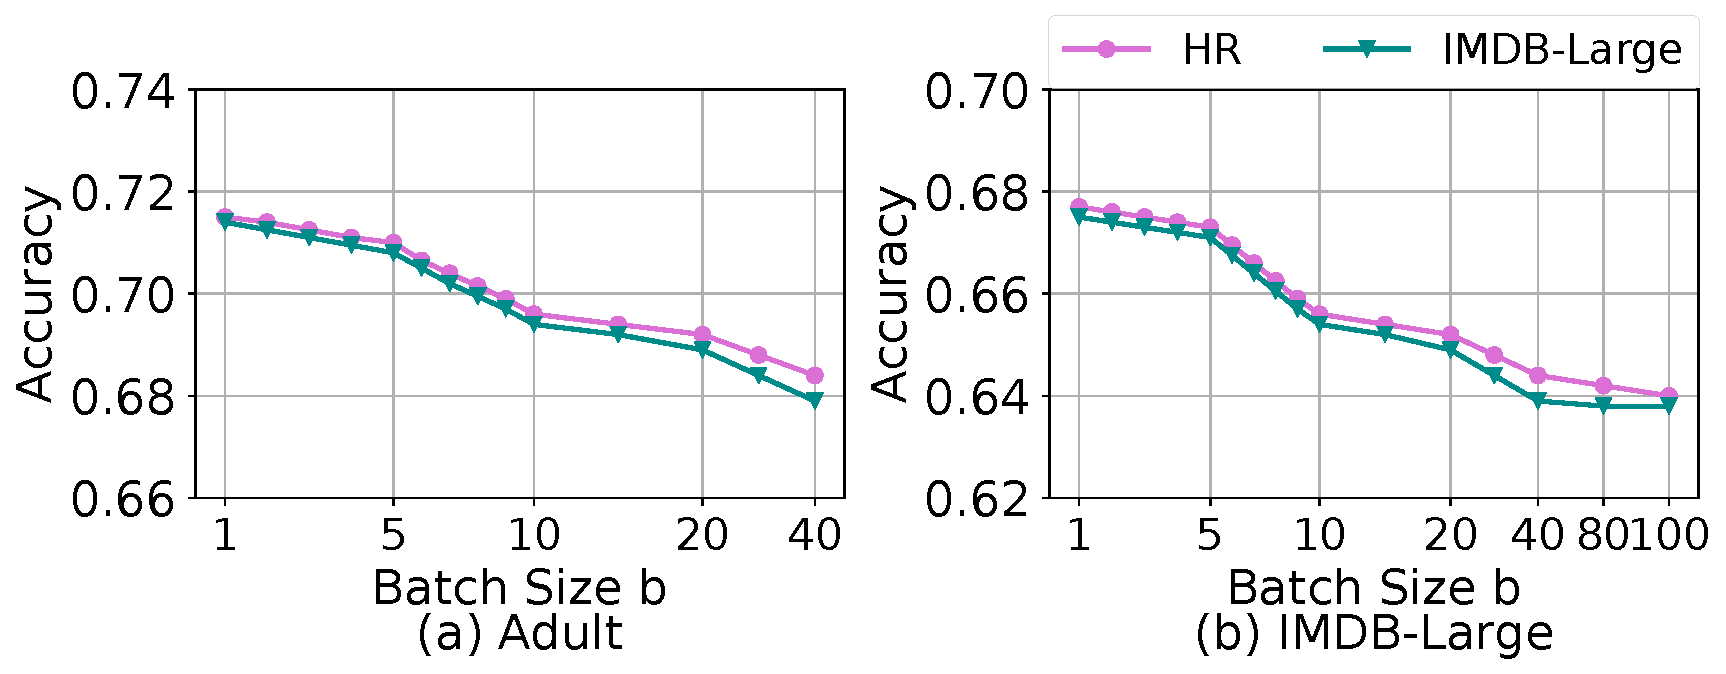
\includegraphics[width=\columnwidth]{figs/batch}
		\vspace{-2.5em}
		\caption{\ours and \ours$^+$ for batch algorithm.}
		\label{fig:batchalg}
	\end{minipage}
	\begin{minipage}[t]{0.32\textwidth}
		\centering
		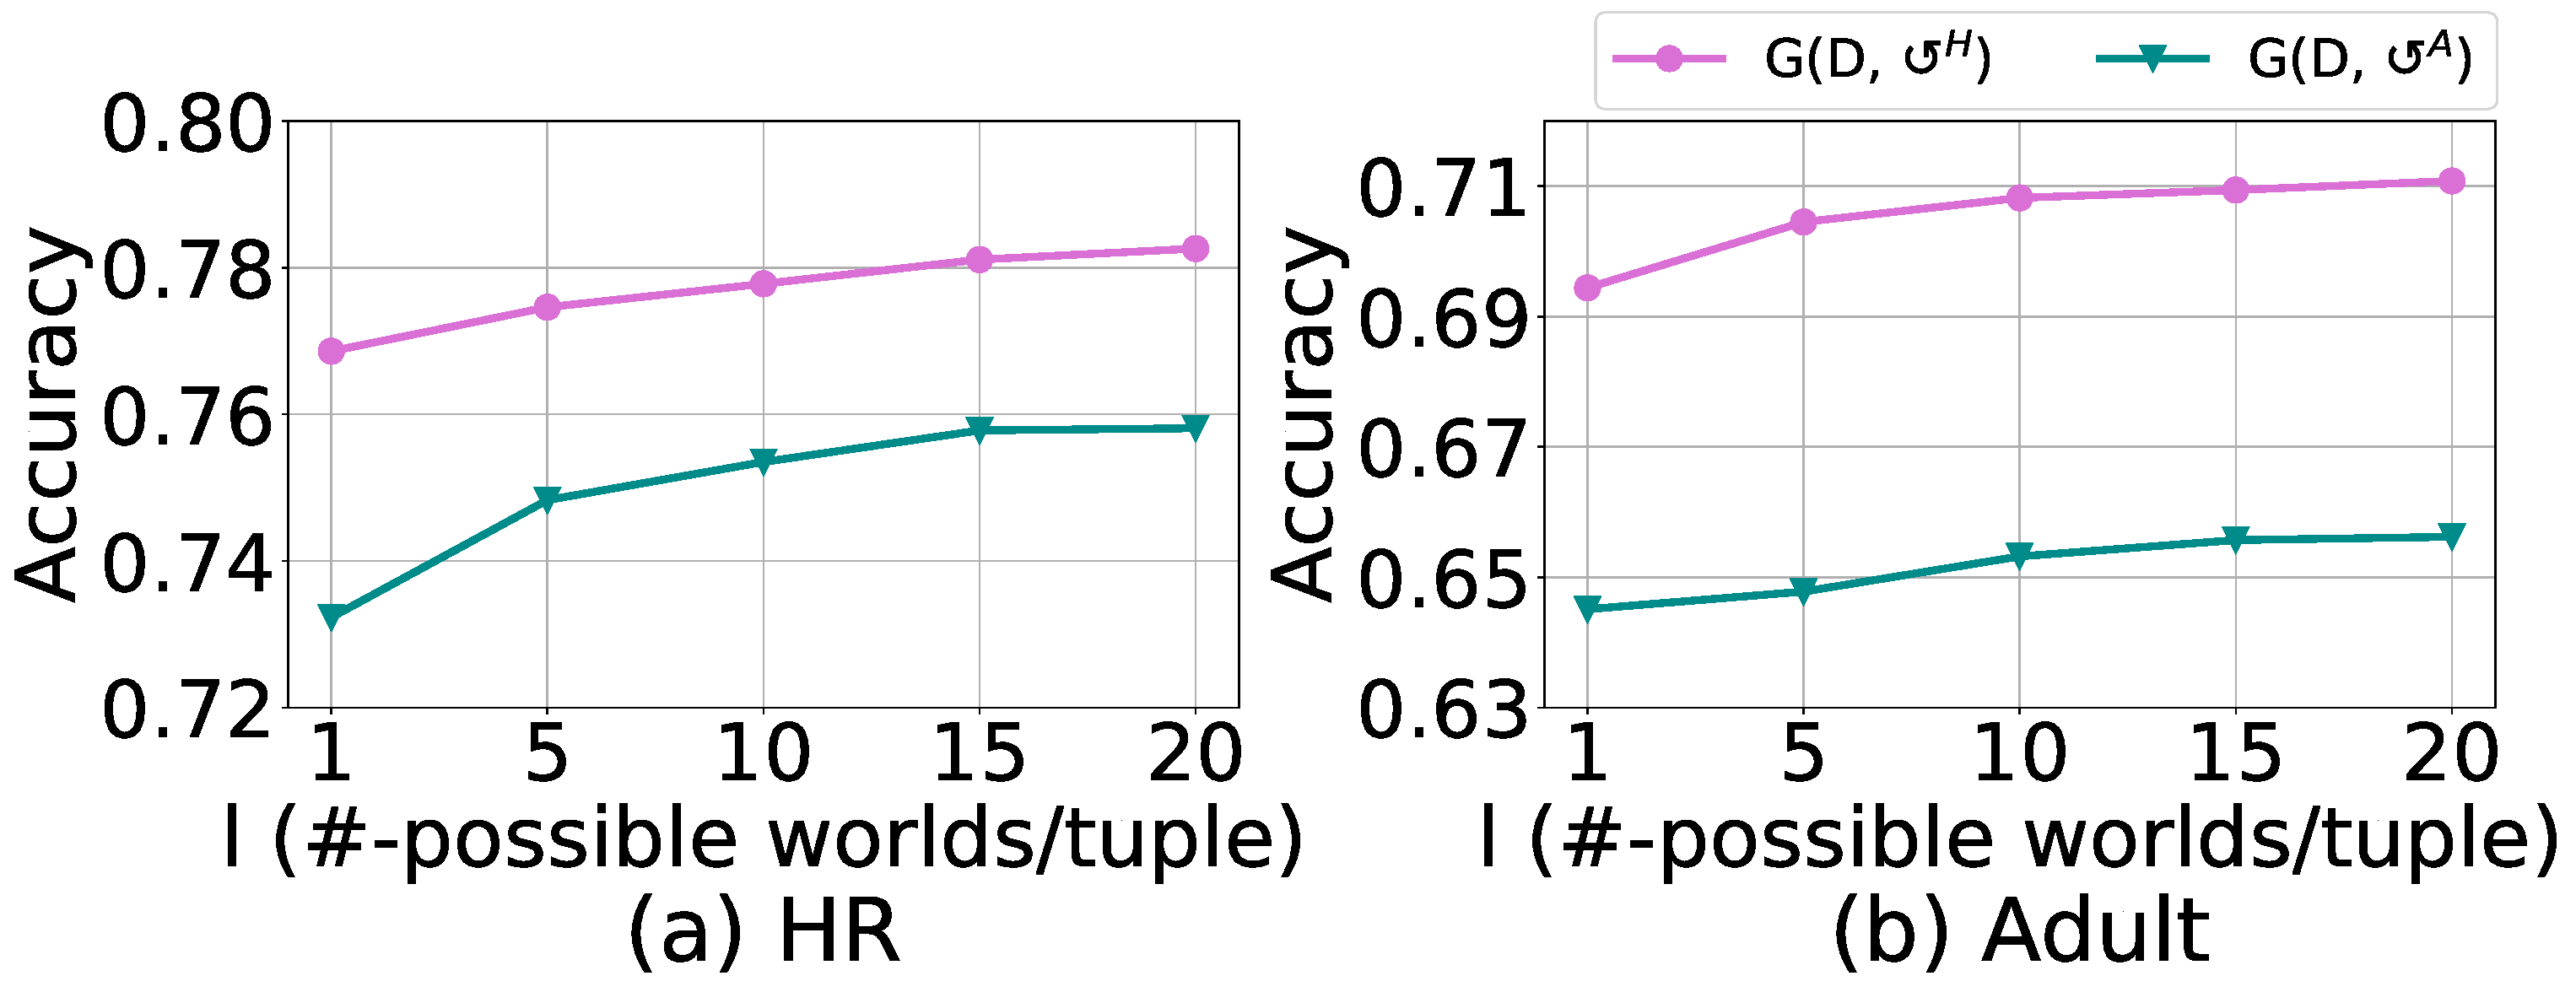
\includegraphics[width=\columnwidth]{figs/vary_l_effectiveness}
		\vspace{-2.5em}
		\caption{Effectiveness of \ours when varying $l$.}
		\label{fig:vary_l_effect}
	\end{minipage}
	\begin{minipage}[t]{0.32\textwidth}
		\centering
		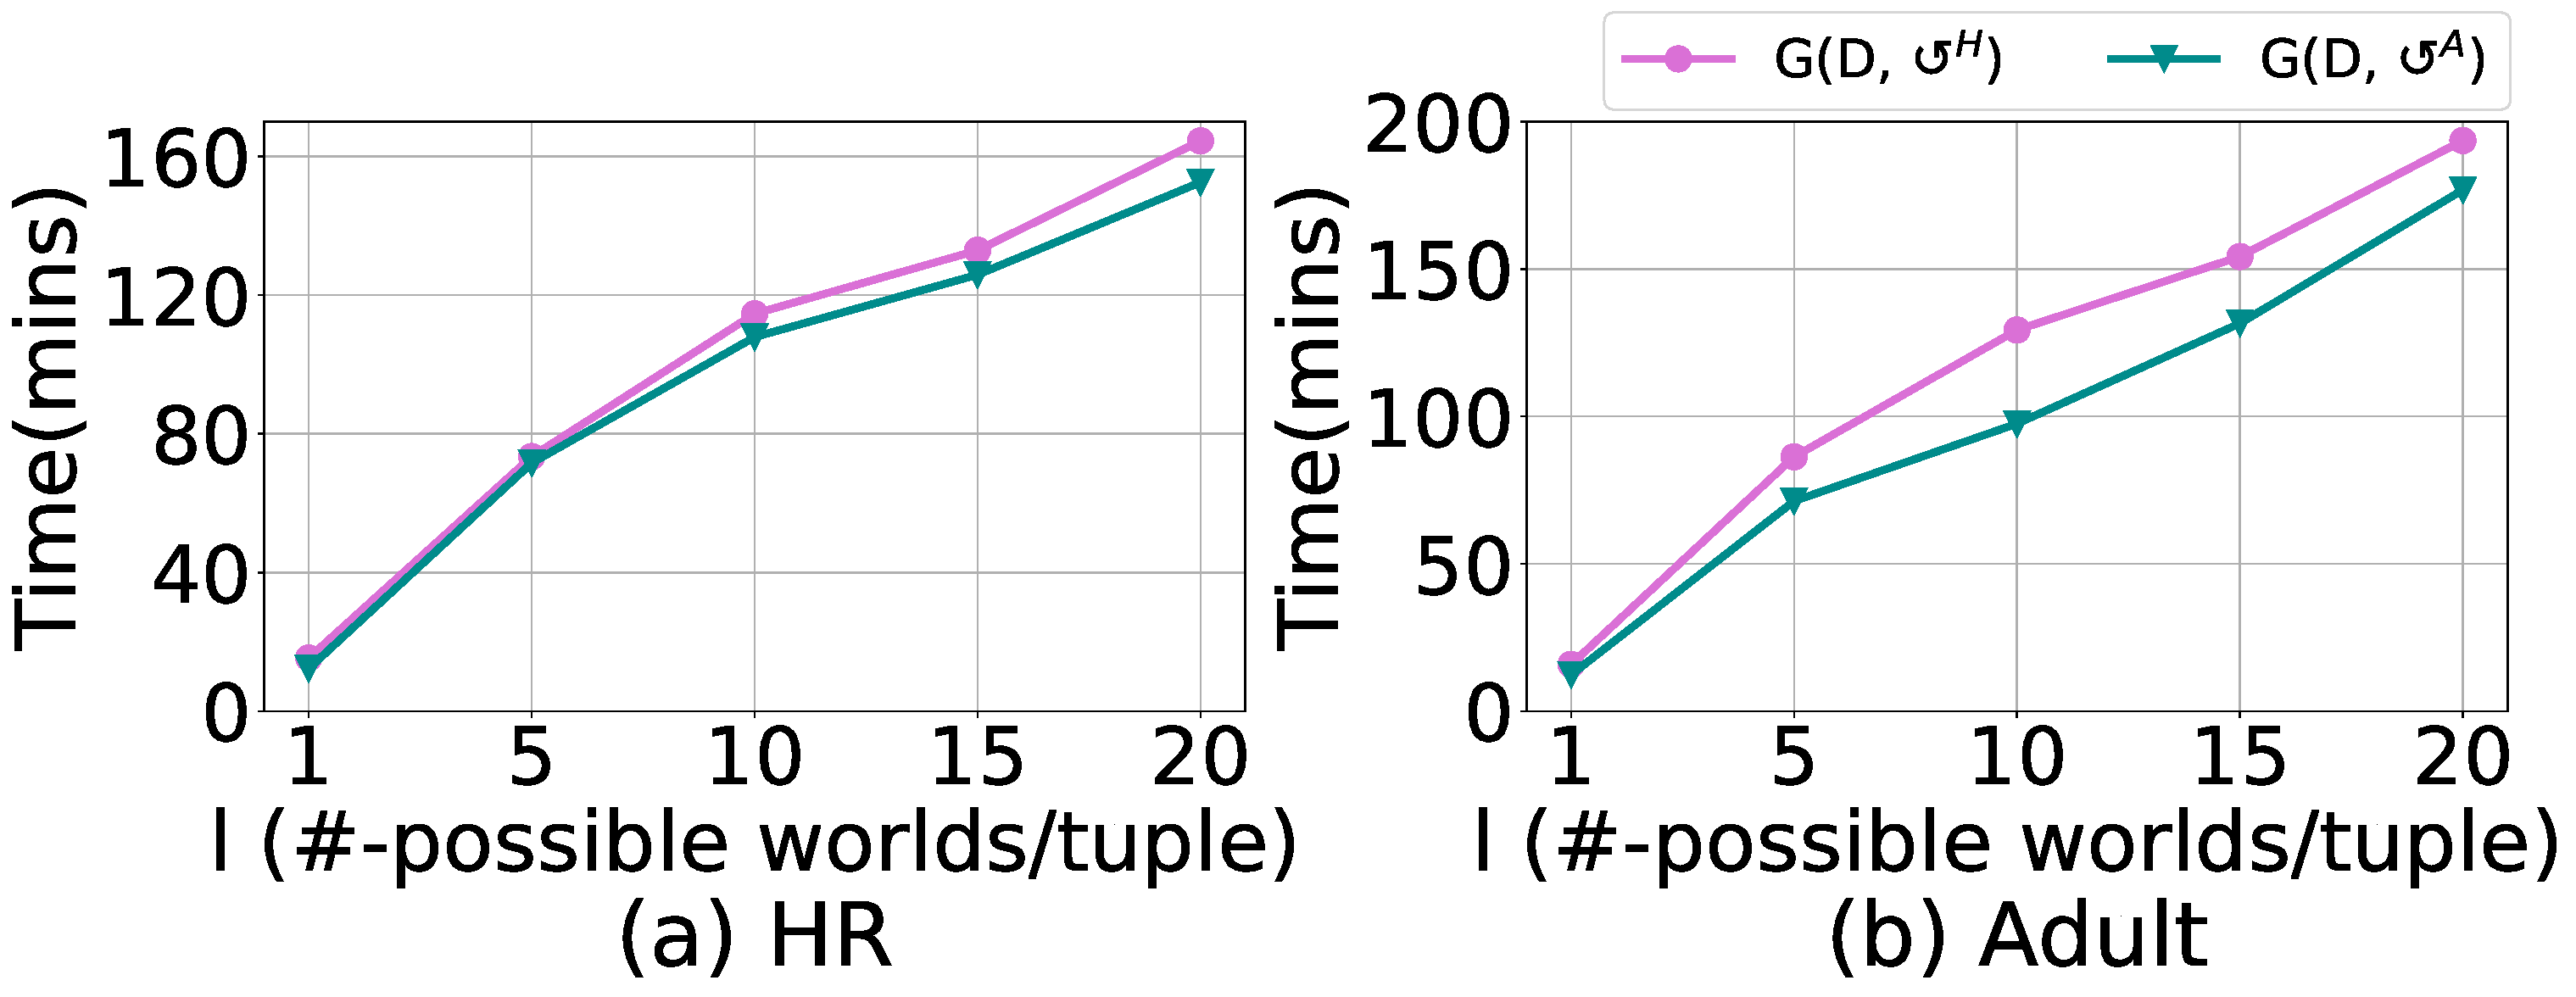
\includegraphics[width=\columnwidth]{figs/vary_l_efficiency}
		\vspace{-2.5em}
		\caption{Efficiency of \ours when varying $l$.}
		\label{fig:vary_l_efficient}
	\end{minipage}
%	\vspace*{-1.8em}   
\end{figure}

% In Figure~\ref{fig:batchalg}, the $x$-axis denotes the batch size and the $y$-axis denotes the test performance on dataset \adult and  \bike. We can see that when $b$ is small (\ie $b \le 5$), the performance does not significantly decrease (\eg on \adult, the accuracy decrease from 71.7\% to 71.2\%.).  When $b$ keeps increasing, the performance slightly decreases. Thus, \ours is not  sensitive to the batch size $b$ and the Algorithm~\ref{alg:batch} can reduce the number of human iterations without sacrificing much  model performance.

\jks{In Figure~\ref{fig:batchalg}, the $x$-axis denotes the batch size and the $y$-axis denotes the test performance on dataset \adult and  \imdbl. We can see that when $b$ is small (\ie $b \le 5$), the performance does not significantly decrease (\eg on \imdbl, the accuracy decrease from 71.5\% to 70.9\% with $seven$.). However, when $b$ keeps increasing, the performance slightly decreases. Thus, \ours  and \ours$^+$ are not sensitive to the batch size $b$ and we can reduce the number of human iterations without sacrificing much  model performance.}


In this part, we also vary the number of possible worlds by varying $l$, which is the number of possibles world per tuple. The larger $l$, the larger number of possible worlds we have. The results are shown in Figures~\ref{fig:vary_l_effect} and  \ref{fig:vary_l_efficient}. In terms of the accuracy, we can see that with $l$ increasing (fixing $b=10$), the accuracy increases first and then  remains stable soon, but the time keeps increasing because more possible worlds indicate more computation. Hence, we do not need a large $l$.

When it comes to the number of possible worlds, we would like to clarify that we do not compare with $\humanfunc(\goodfunc(\train))$ and $\autofunc(\goodfunc(\train))$ because  the number of  possible worlds of $\train$ is very large, which is infeasible to compute. We show the number in Table~\ref{tbl:pwnum}, where we also report the numbers of possible worlds of $\seven$ and $\eight$ in each iteration, which are practical to compute.


\begin{table}
	\centering
	\caption{The number of possible worlds on different datasets}
	{\small
		\begin{tabular}{cccc}
			\hline
			{\bf Method} & {\bf \nursery} & {\bf \hr} & {\bf \adult} \\
			\hline	
			$\five$ & $10^{201}$ & $10^{201}$ & $10^{202}$ \\
			$\six$ & $10^{201}$ & $10^{201}$ & $10^{202}$ \\
			$\seven$ & $10^3$ & $10^3$ & $10^4$ \\
			$\eight$ & $10^3$ & $10^3$ & $10^4$ \\
			\hline
		\end{tabular}
	}
	\label{tbl:pwnum}
	\vspace{-1em}
\end{table}



%!TEX root = ../main.tex

\begin{figure}
	\centering
	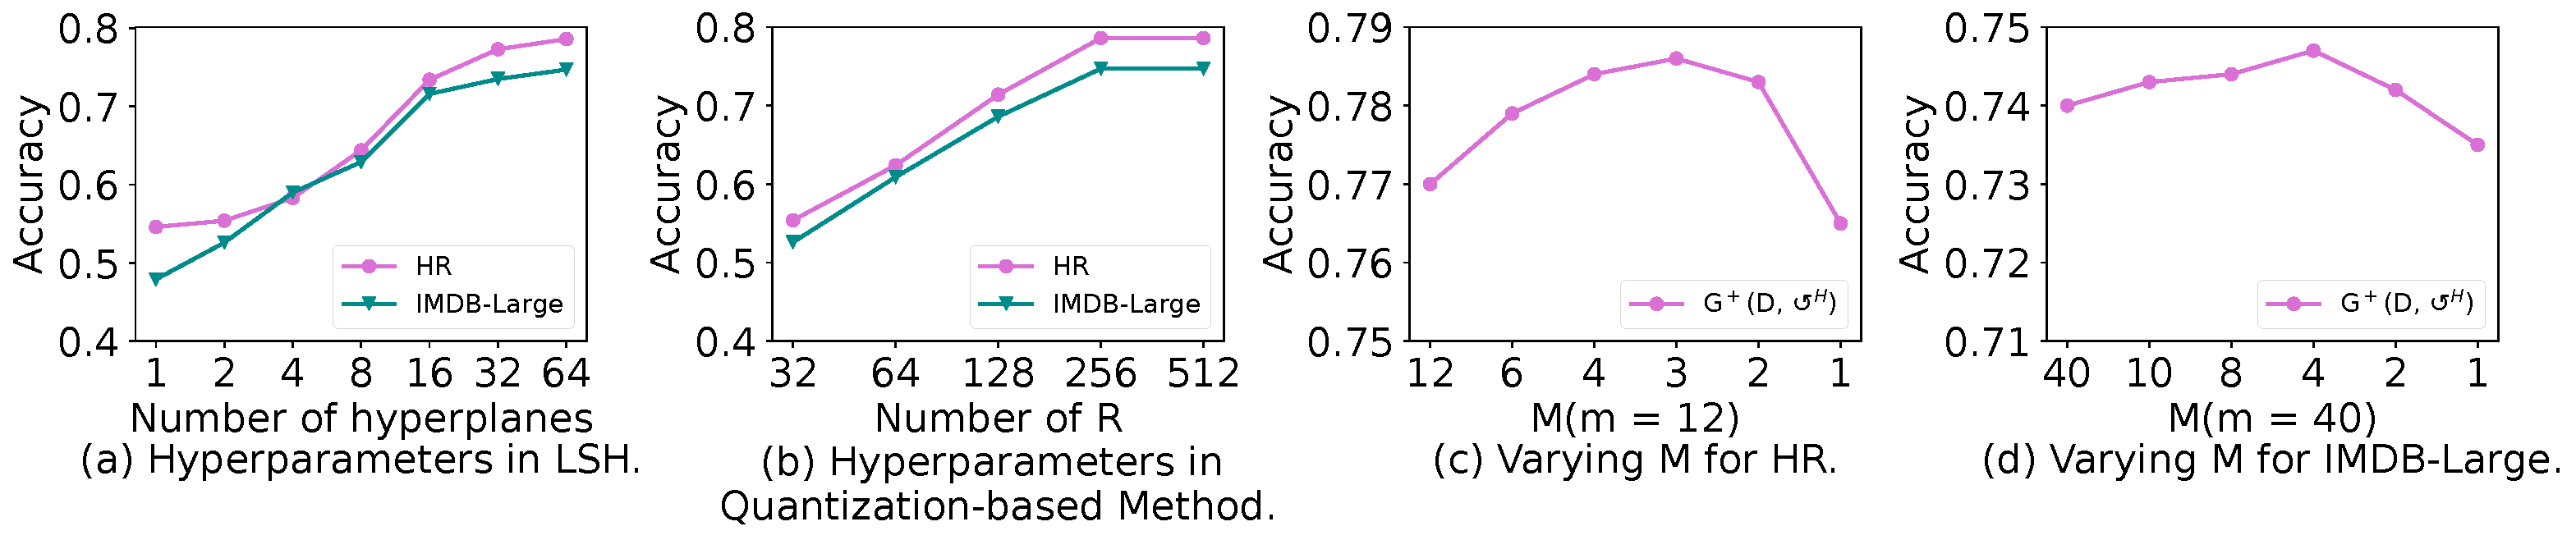
\includegraphics[width=1\textwidth]{figs/M}
	\vspace{-1em}
	\caption{Varying Hyperparameters in LSH and Quantization-based Method.}
	\label{fig:pq-exp}
	\vspace{-1em}
\end{figure}

\subsection{Ablation Studies of \texttt{GoodCore}$^+$}
\noindent{\bf Hyperparamaters for grouping.}
%
We use LSH to efficiently group the entire dataset, and test the impact of  different numbers of hyperplanes, which is a significant parameter in LSH.
 As shown in Figure~\ref{fig:pq-exp} (a), with the number increasing, more groups are generated, and the tuples within each cluster are closer, so the  accuracy increases at the beginning. Afterwards, the accuracy remains stable because tuples in each cluster are similar enough for  approximating the gradient. Therefore, empirically, using  64 hyperplanes is the most appropriate because more groups will reduce the efficiency.

\noindent{\bf Hyperparamaters in quantization-based method.} In Section~\ref{subsec:pq}, we use quantization-based method to estimate the upper bound $\hat{s}_{ju}$ of $\overline{s}_{ju}$. Recap that \texttt{GoodCore}$^+$ needs the user-specified cluster centers size $R$, which is important for computing the maximum feature distances.
%
 To choose a proper $R$, we adopt a simple yet effective solution that selects different $R$ and obtain different coresets. Then we train over these coresets and evaluate via a validation set to get different results. Specifically, we select $R$ from 32 to 512 for each dataset. Figure~\ref{fig:pq-exp} (b) shows the performance on dataset \hr and \imdbl when varying the cluster centers size $R$.  We can see that as $R$ increases, the accuracy of the dataset also gradually increases, because when $R$ increases, the upper bound $\hat{s}_{ju}$ is closer to $\overline{s}_{ju}$, which can help us to select a good coreset.


We also test the performance of different feature splitting ways (corresponding to different $M$). In Figure~\ref{fig:pq-exp}(c)-(d), initially,  $M=12$ indicates that in each subspace, the length of all sub-vectors is 1. With $M$ decreasing, the accuracy increases first because each sub-vector becomes longer, which contains more information when adding up these $\hat{s}^z_{ju}$, leading to a more precise bound. But if each sub-vector is too long, which means that each vector is quantized to a very short code, the accuracy decreases because in this situation, the quantization-based method is not informative enough to give accurate  distance estimation. Empirically, when $M$ is around 3, it is always a good choice.

\noindent{\bf Varying the entropy threshold.} 
\begin{figure}[t]   
	\centering
	\begin{minipage}[t]{0.49\textwidth}
		\centering
		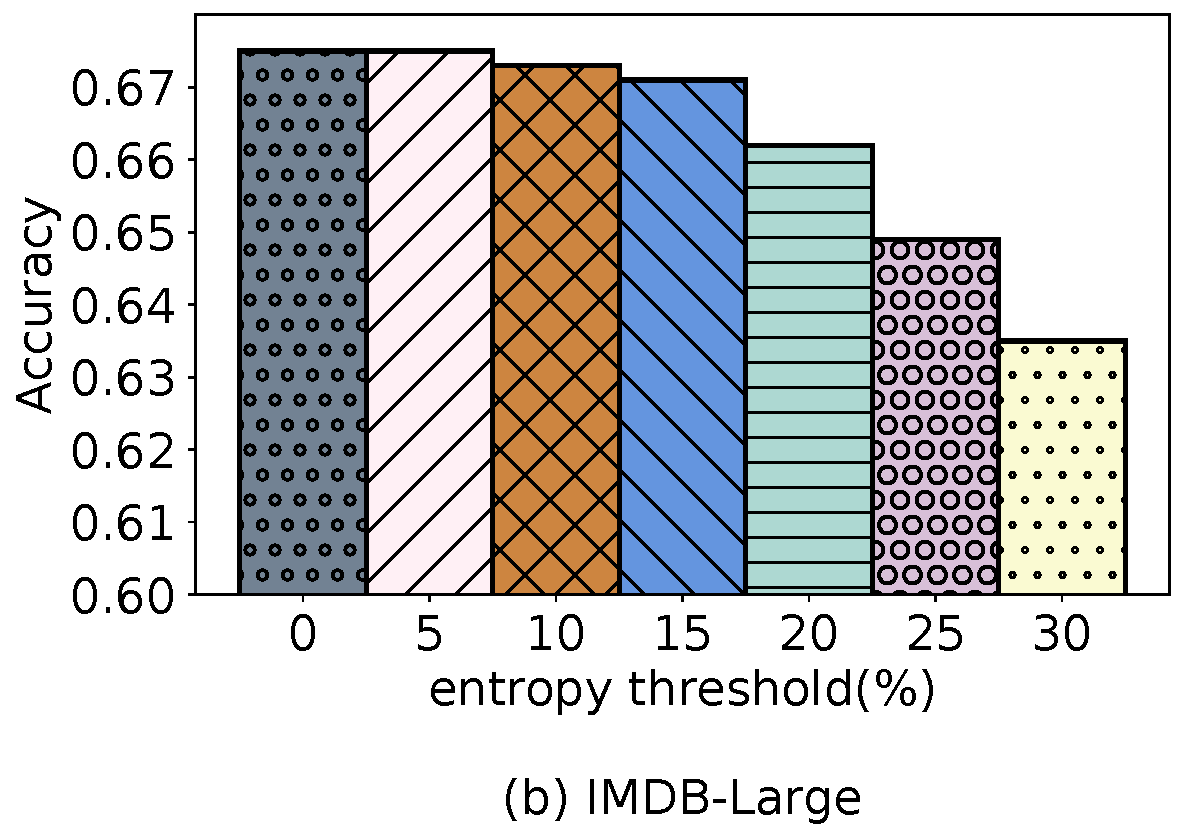
\includegraphics[width=\columnwidth]{figs/entropy_acc}
		\vspace{-1.5em}
		\caption{Effectiveness of \ours$^+$ for different Threshold.}
		\label{fig:entropy_acc}
	\end{minipage}
	\begin{minipage}[t]{0.49\textwidth}
		\centering
		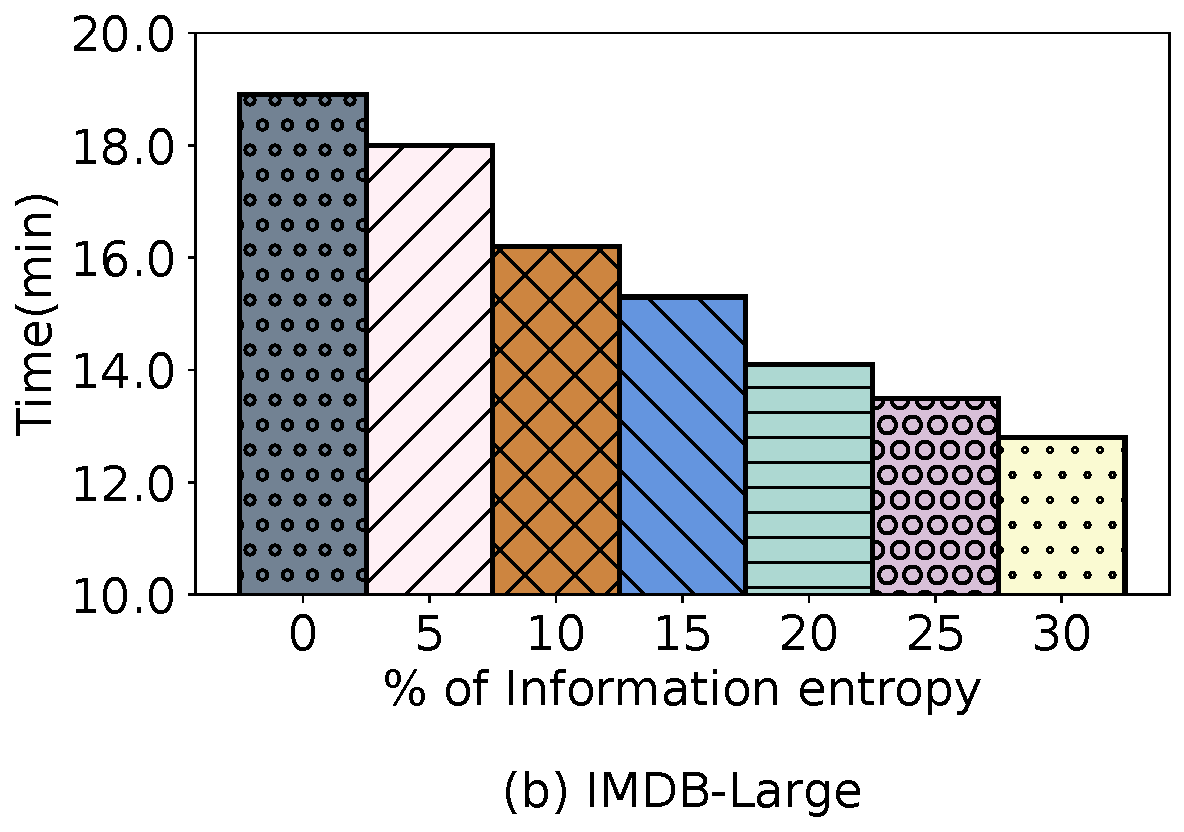
\includegraphics[width=\columnwidth]{figs/entropy_time}
		\vspace{-1.5em}
		\caption{Efficiency of \ours$^+$ for different Threshold.}
		\label{fig:entropy_time}
	\end{minipage}
	\vspace*{-1em}   
\end{figure}
%
In this part, we start to use the entropy to further eliminate the number of possible world by imputing the missing cells with low entropy in advance, as discussed in Section~\ref{subsec:clustering}. 
%
Specifically, we test the impact of different entropy thresholds. As shown in Figure~\ref{fig:entropy_acc}, when the threshold is less than  15\% (\ie we directly impute the cell if its corresponding entropy is no larger than 15\% $\log n_x$), the accuracy almost remains unchanged, but the efficiency is improved by up to \cc{XX\%}. However, when the threshold exceeds 15\%, the accuracy begins to decrease because in this situation, directly imputing a value is not accurate enough. In short, setting an appropriate threshold (\eg 15\%) is helpful to improve the efficiency without sacrificing the accuracy. 

% rate of decrease accelerates. This is because when the threshold is low, all the candidate words filled in for the missing values have a high probability(\ie 90\%) and the threshold increases, the maximum probability gradually decreases, making the selection of candidate words for missing values more challenging. For example, on dataset \imdbl, when threshold is 15\%, the accuracy of \ours$^+$ is 71\%, which is only 0.4\% lower than when no processing is done at all.

%Furthermore, we report the time change to reflect the efficiency of \ours$^+$ for different thresholds of information entropy. In Figure~\ref{fig:entropy_time}, we can see that the algorithm spends less and less time as the threshold increases because of the reduction in the number of incomplete tuples. On dataset \imdbl, when threshold is 30\%, the runtime of \ours$^+$ has decreased by over 30\%. And the runtime of \ours$^+$ decreased by approximately 3 minutes when threshold is 15\%.
%
%In summary, we can use a appropriate threshold of information entropy to preemptively fill in some missing values, which can effectively reduce the runtime of \ours$^+$ while ensuring accuracy. 


\begin{figure}
	\centering
	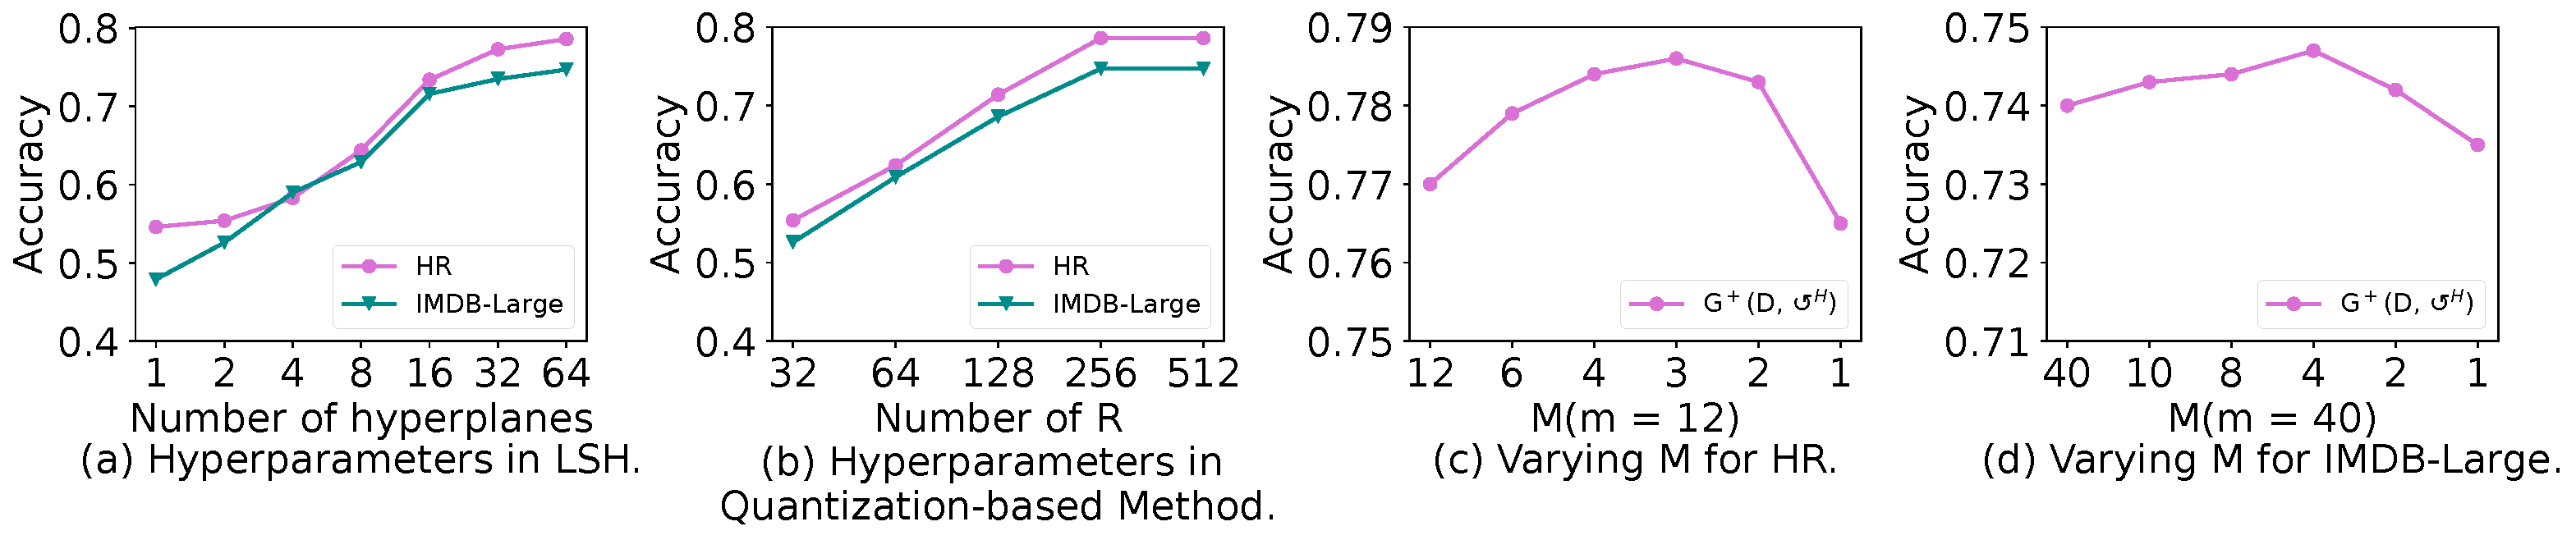
\includegraphics[width=1\textwidth]{figs/M}
%	\vspace{-1em}
	\caption{Varying Hyperparameters in LSH and PQ.}
	\label{fig:pq-exp}
%	\vspace{-1em}
\end{figure}

%!TEX root = ../main.tex
\vspace{-0.5em}
\subsection{Convergence Evaluation}

\begin{figure}[t]   
	\centering
	\begin{minipage}[t]{0.49\textwidth}
		\centering
		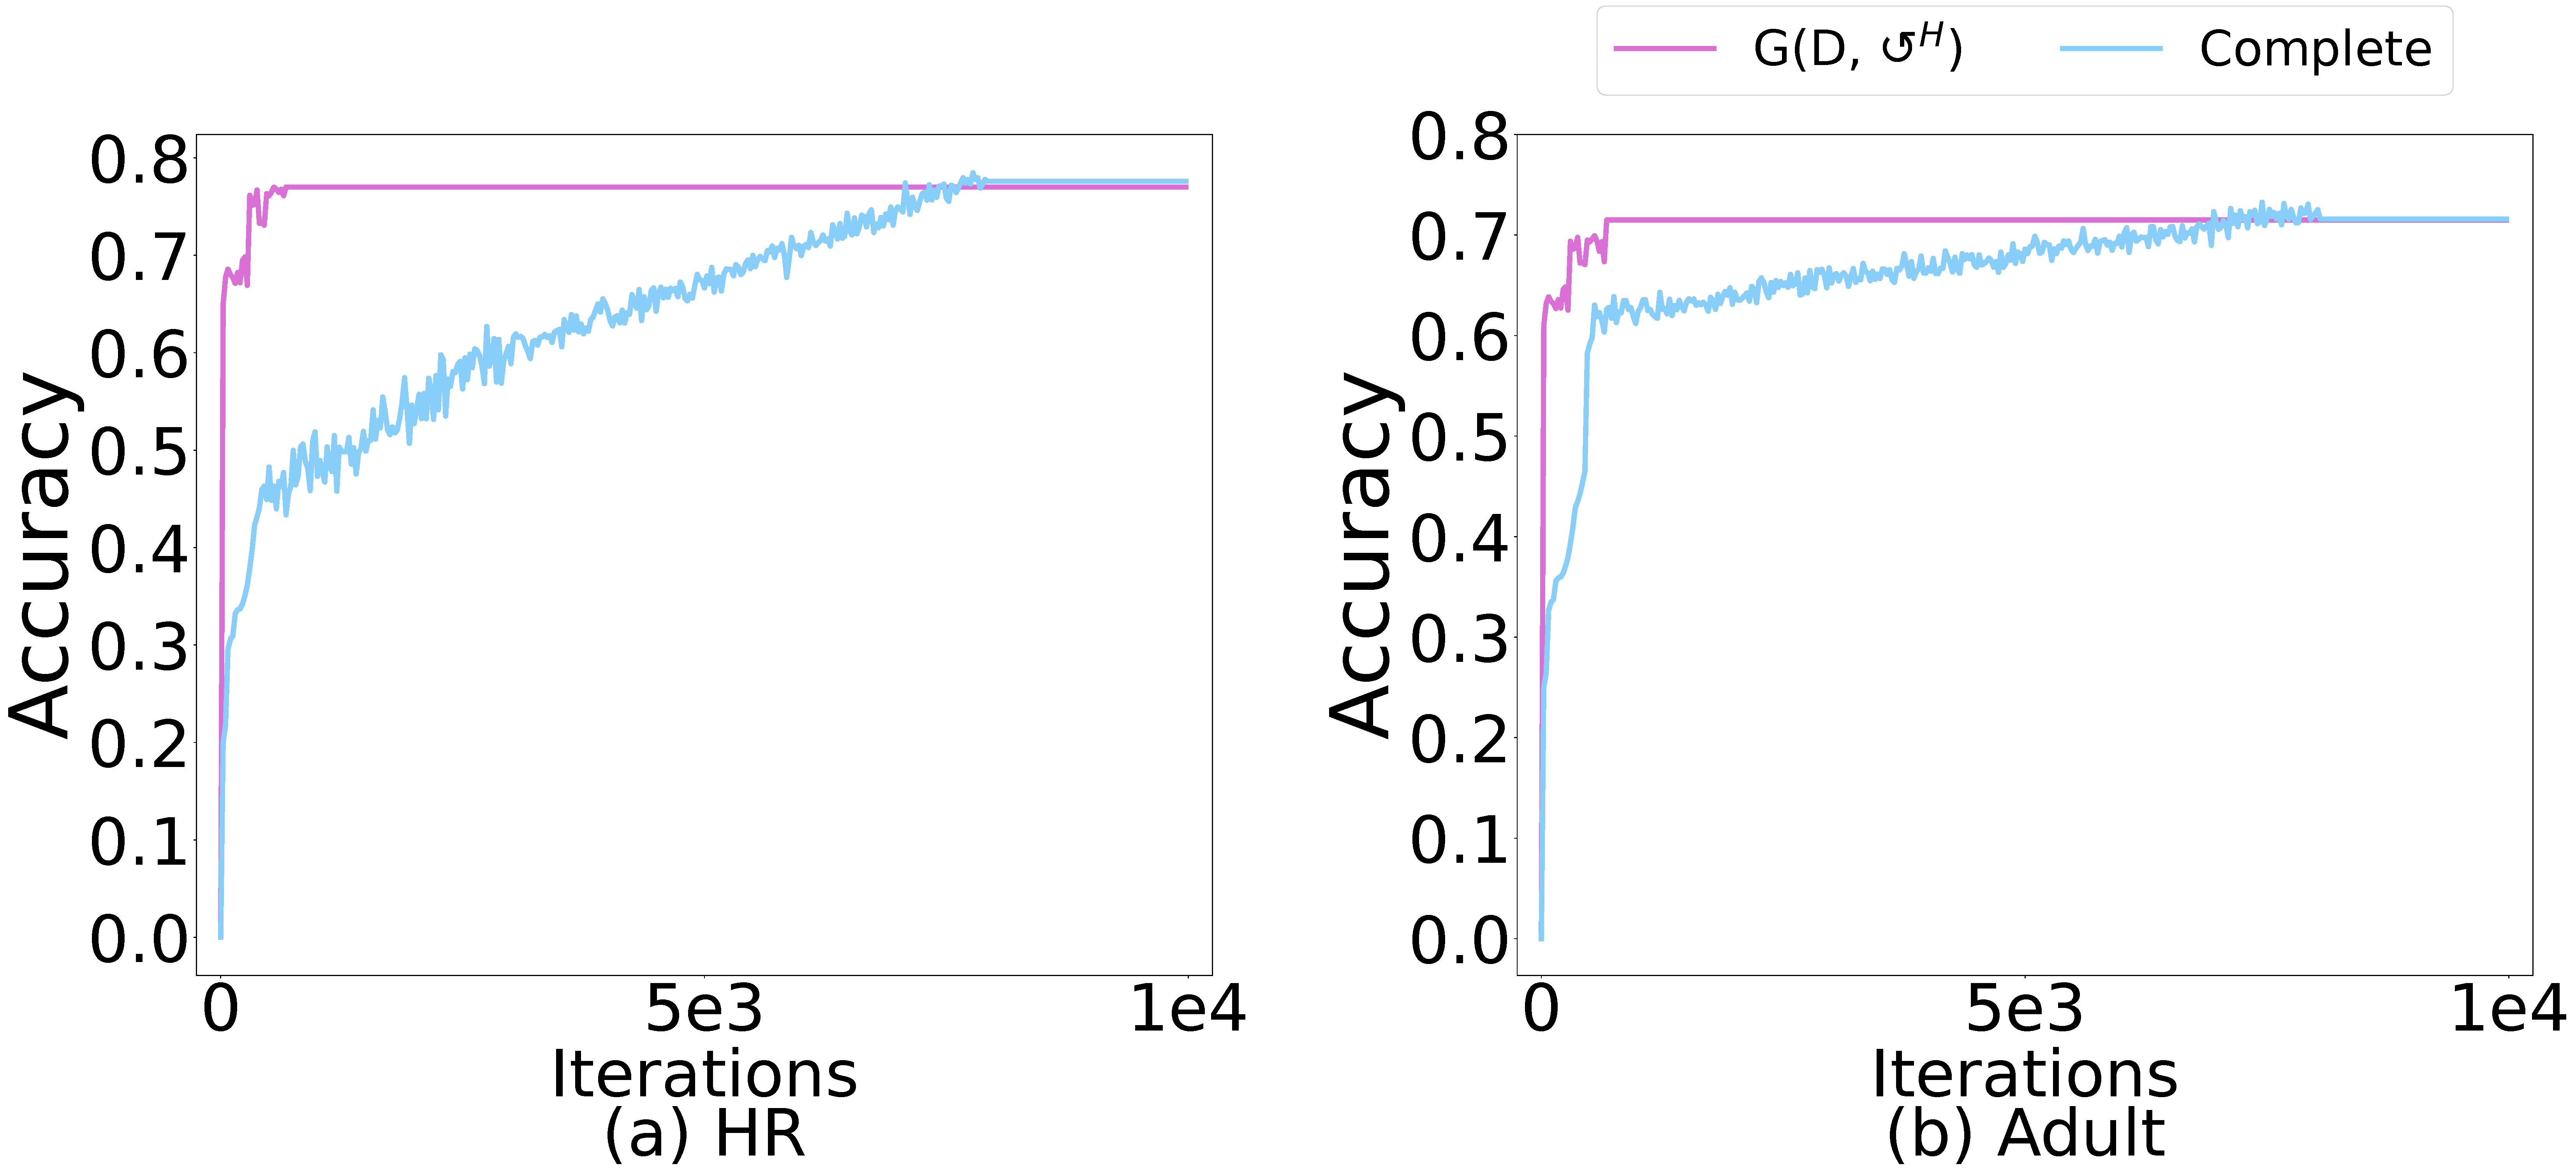
\includegraphics[width=\columnwidth]{figs/G_a}
	    \vspace{-1.5em}
		\caption{Convergence of \ours.}
		\label{fig:converge_G}
	\end{minipage}
	\begin{minipage}[t]{0.49\textwidth}
		\centering
		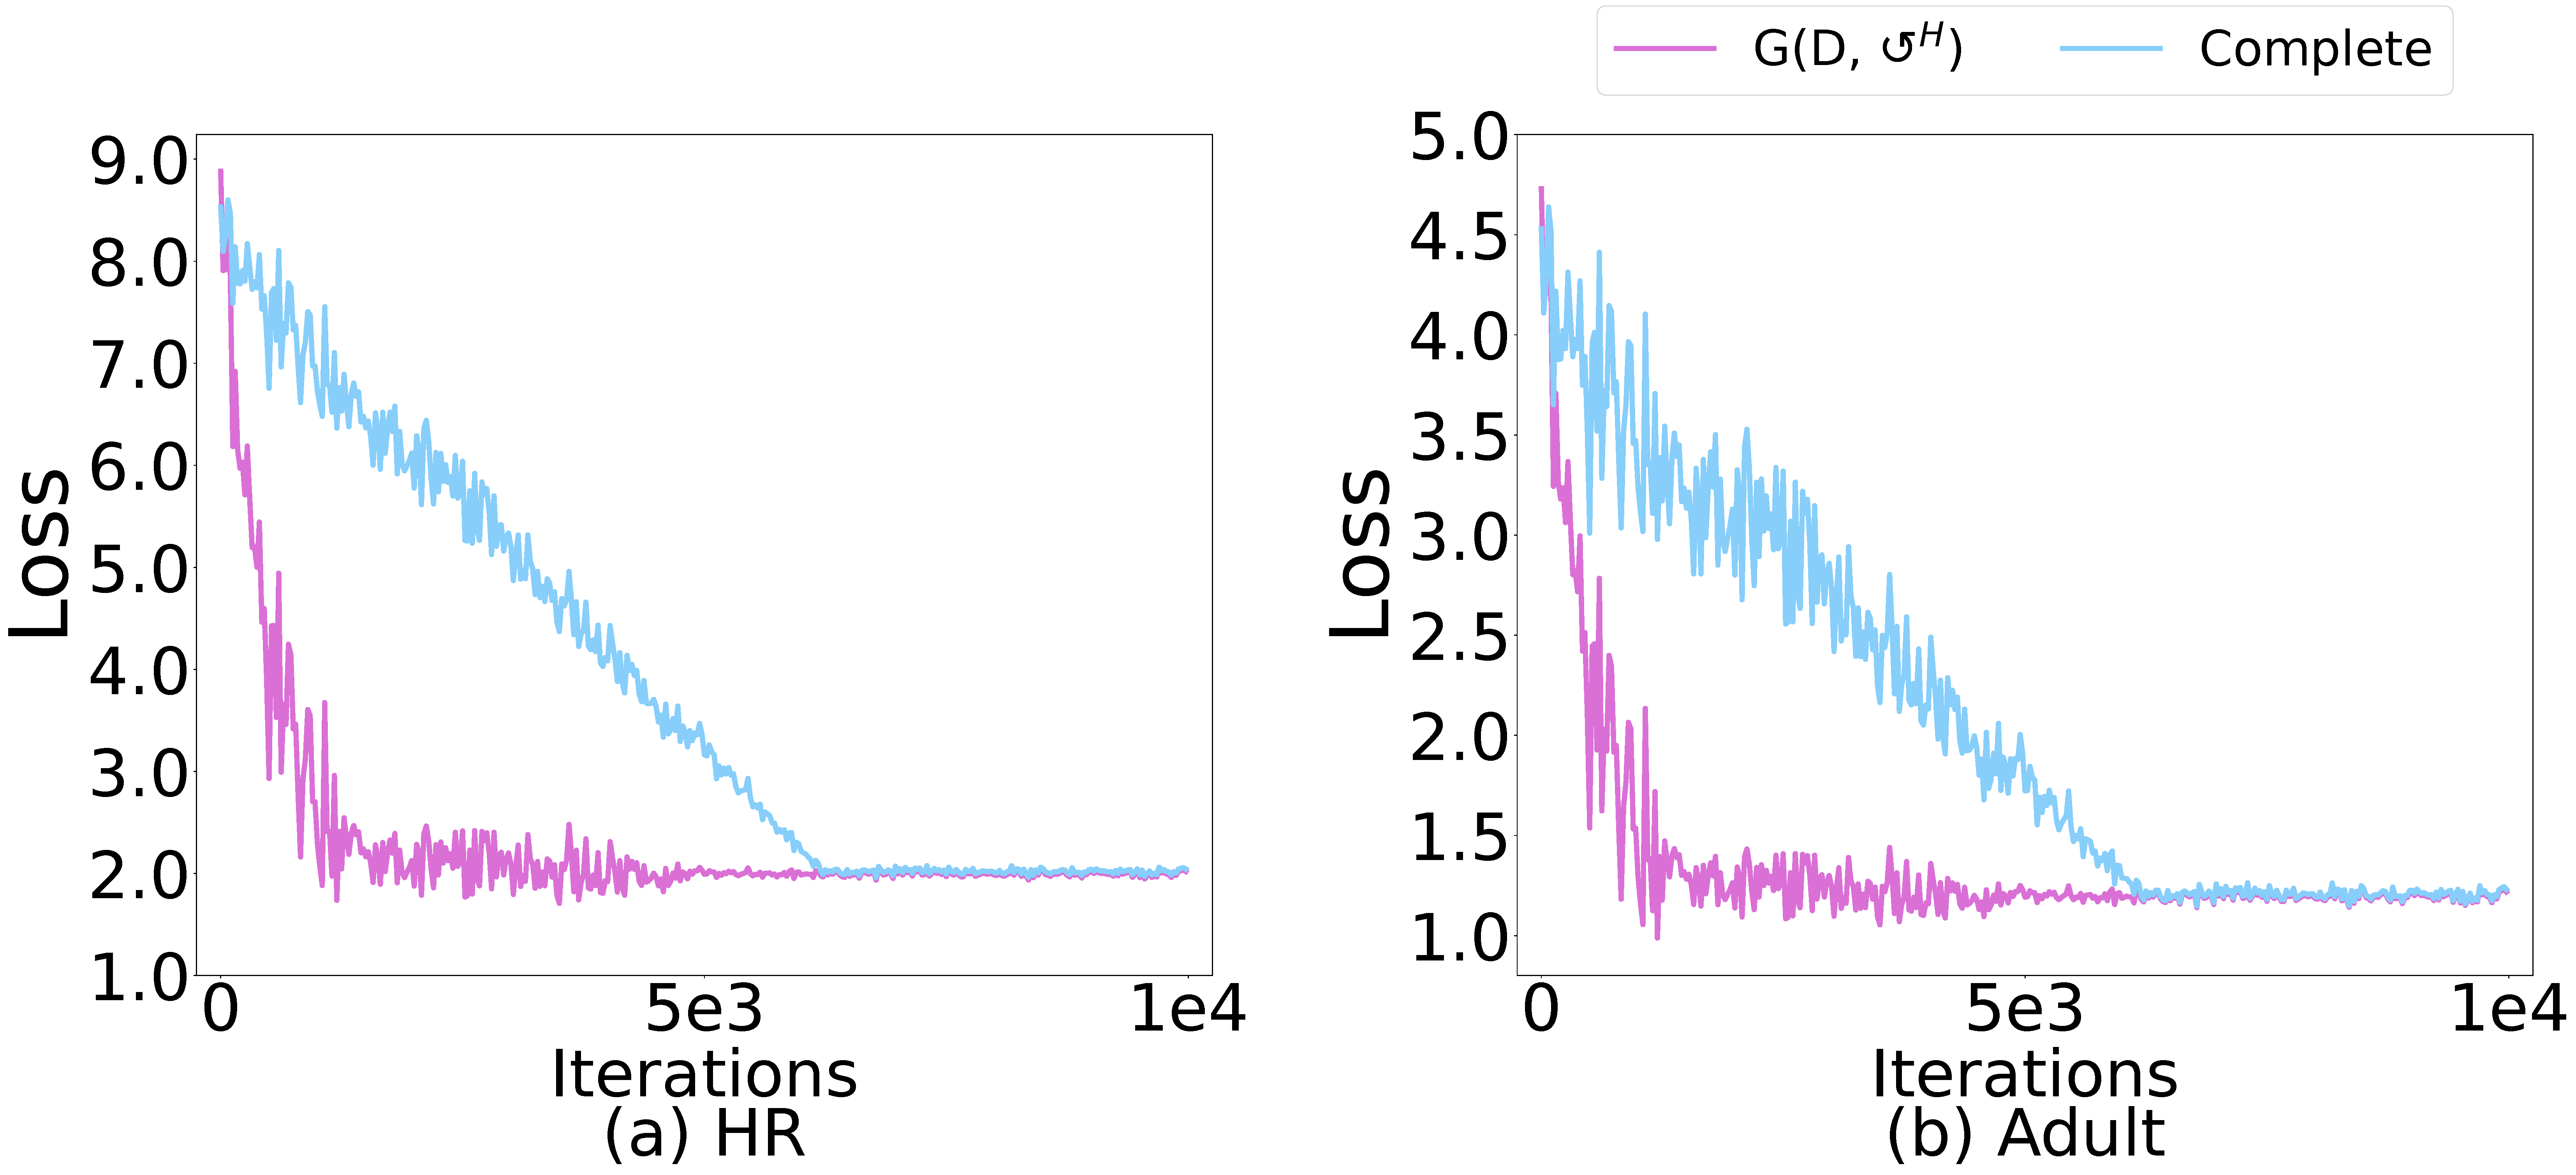
\includegraphics[width=\columnwidth]{figs/G}
	    \vspace{-1.5em}
		\caption{Loss of \ours.}
		\label{fig:real_loss_G}
	\end{minipage}
	\vspace*{-1em}   
\end{figure}

\begin{figure}[t]   
	\centering
	\begin{minipage}[t]{0.49\textwidth}
		\centering
		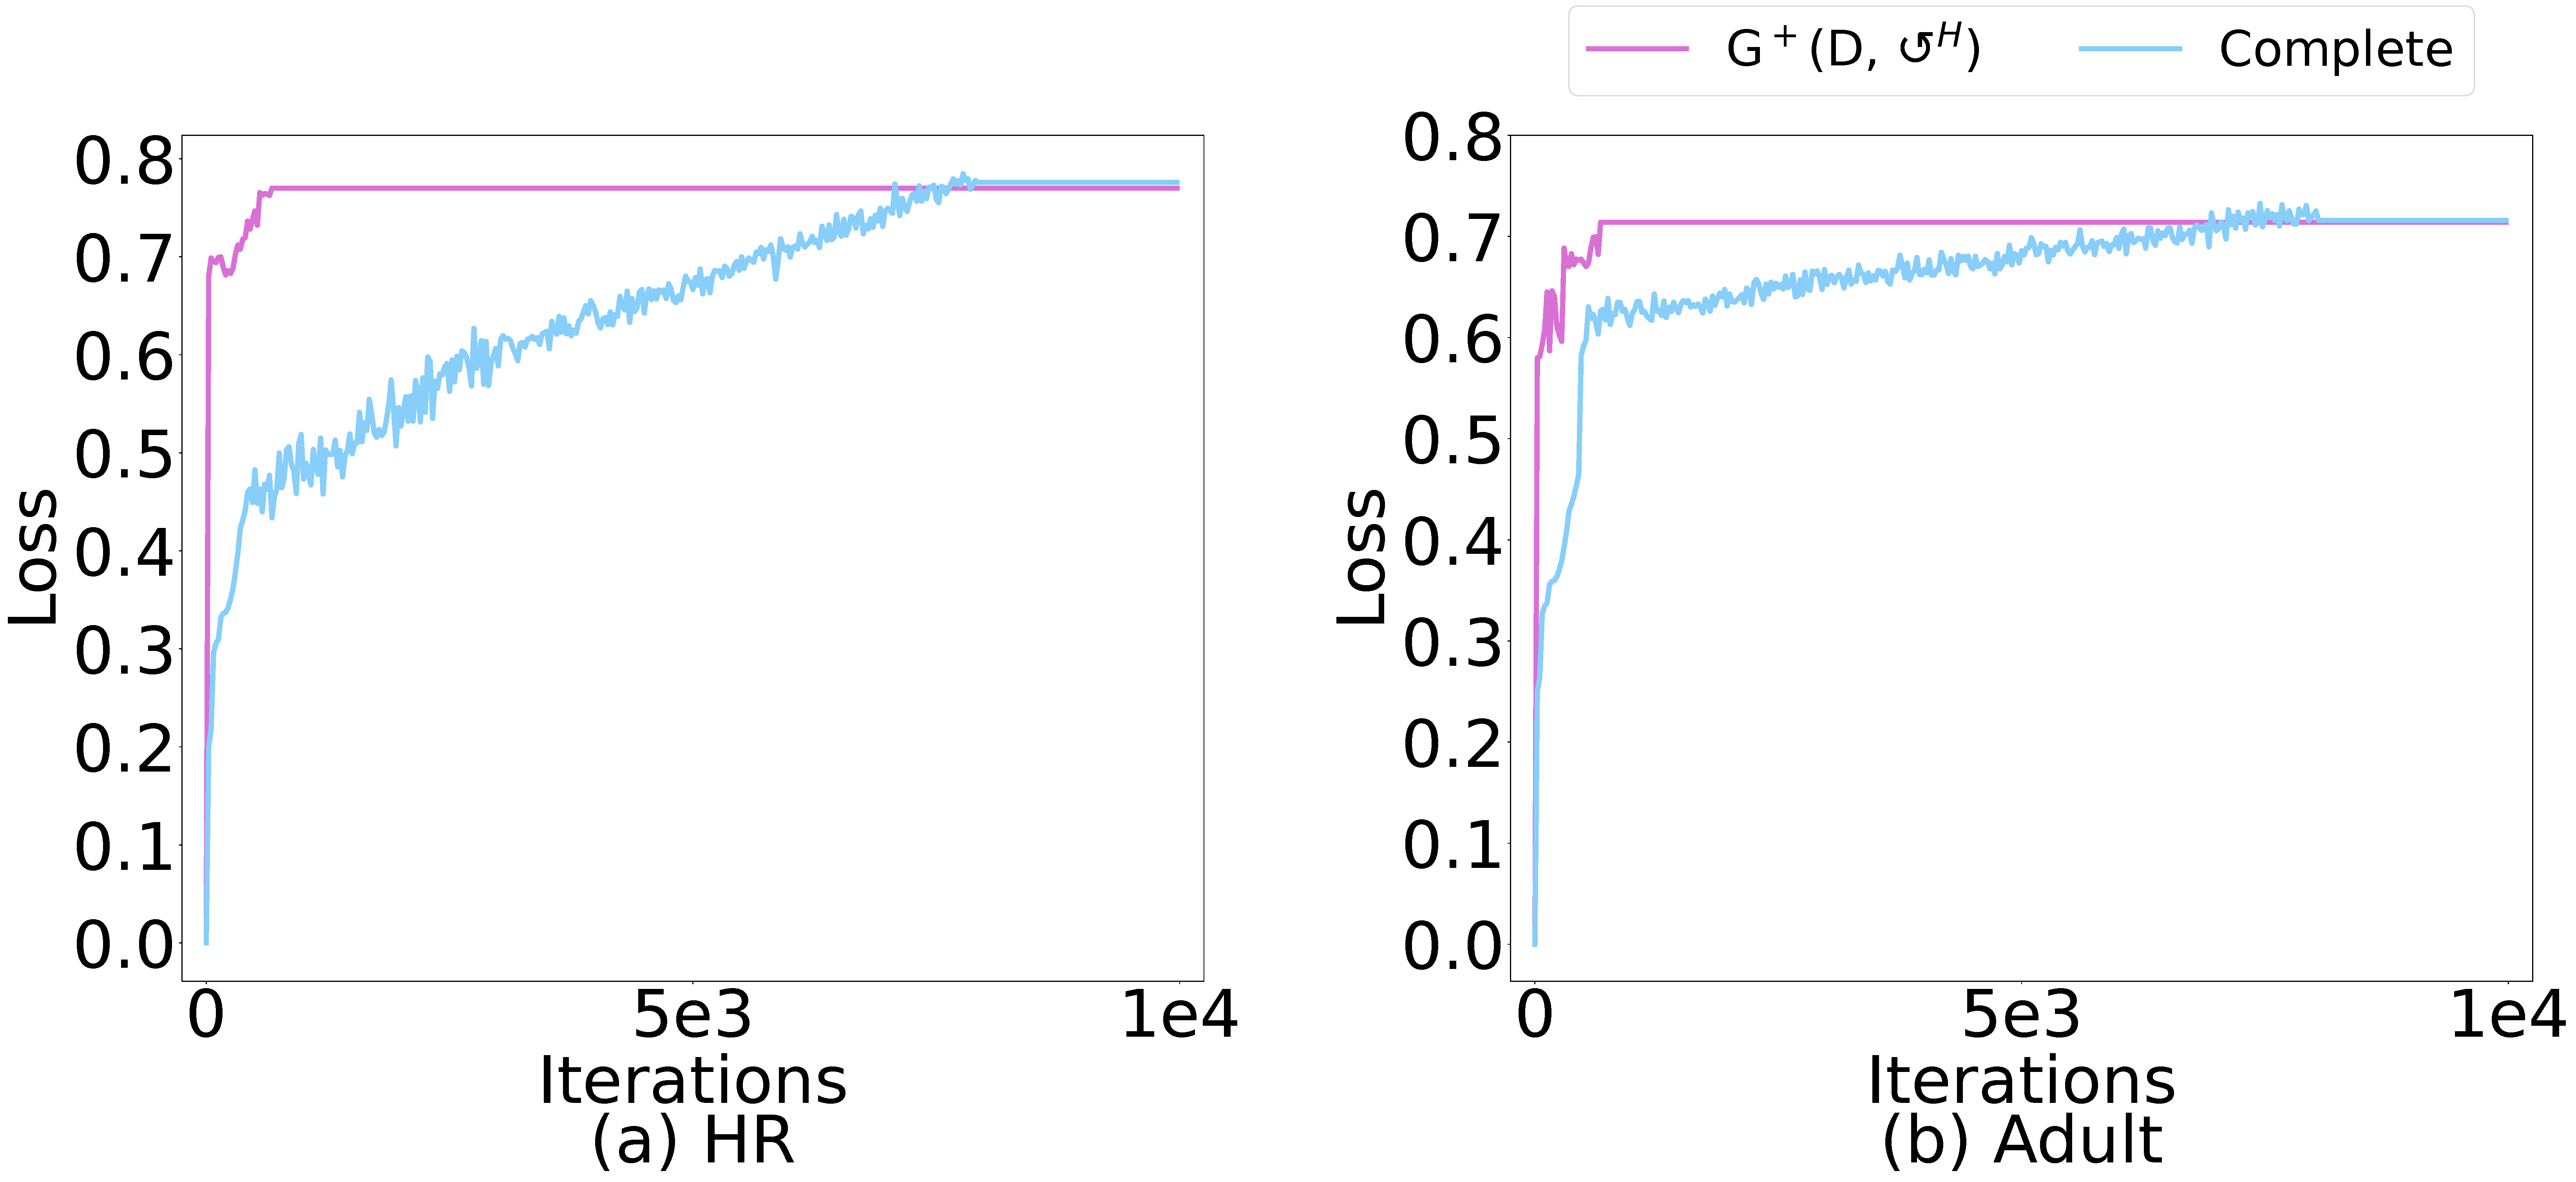
\includegraphics[width=\columnwidth]{figs/G+_a}
		\vspace{-1.5em}
		\caption{Convergence of \texttt{GoodCore}$^+$.}
		\label{fig:converge_G+}
	\end{minipage}
	\begin{minipage}[t]{0.49\textwidth}
		\centering
		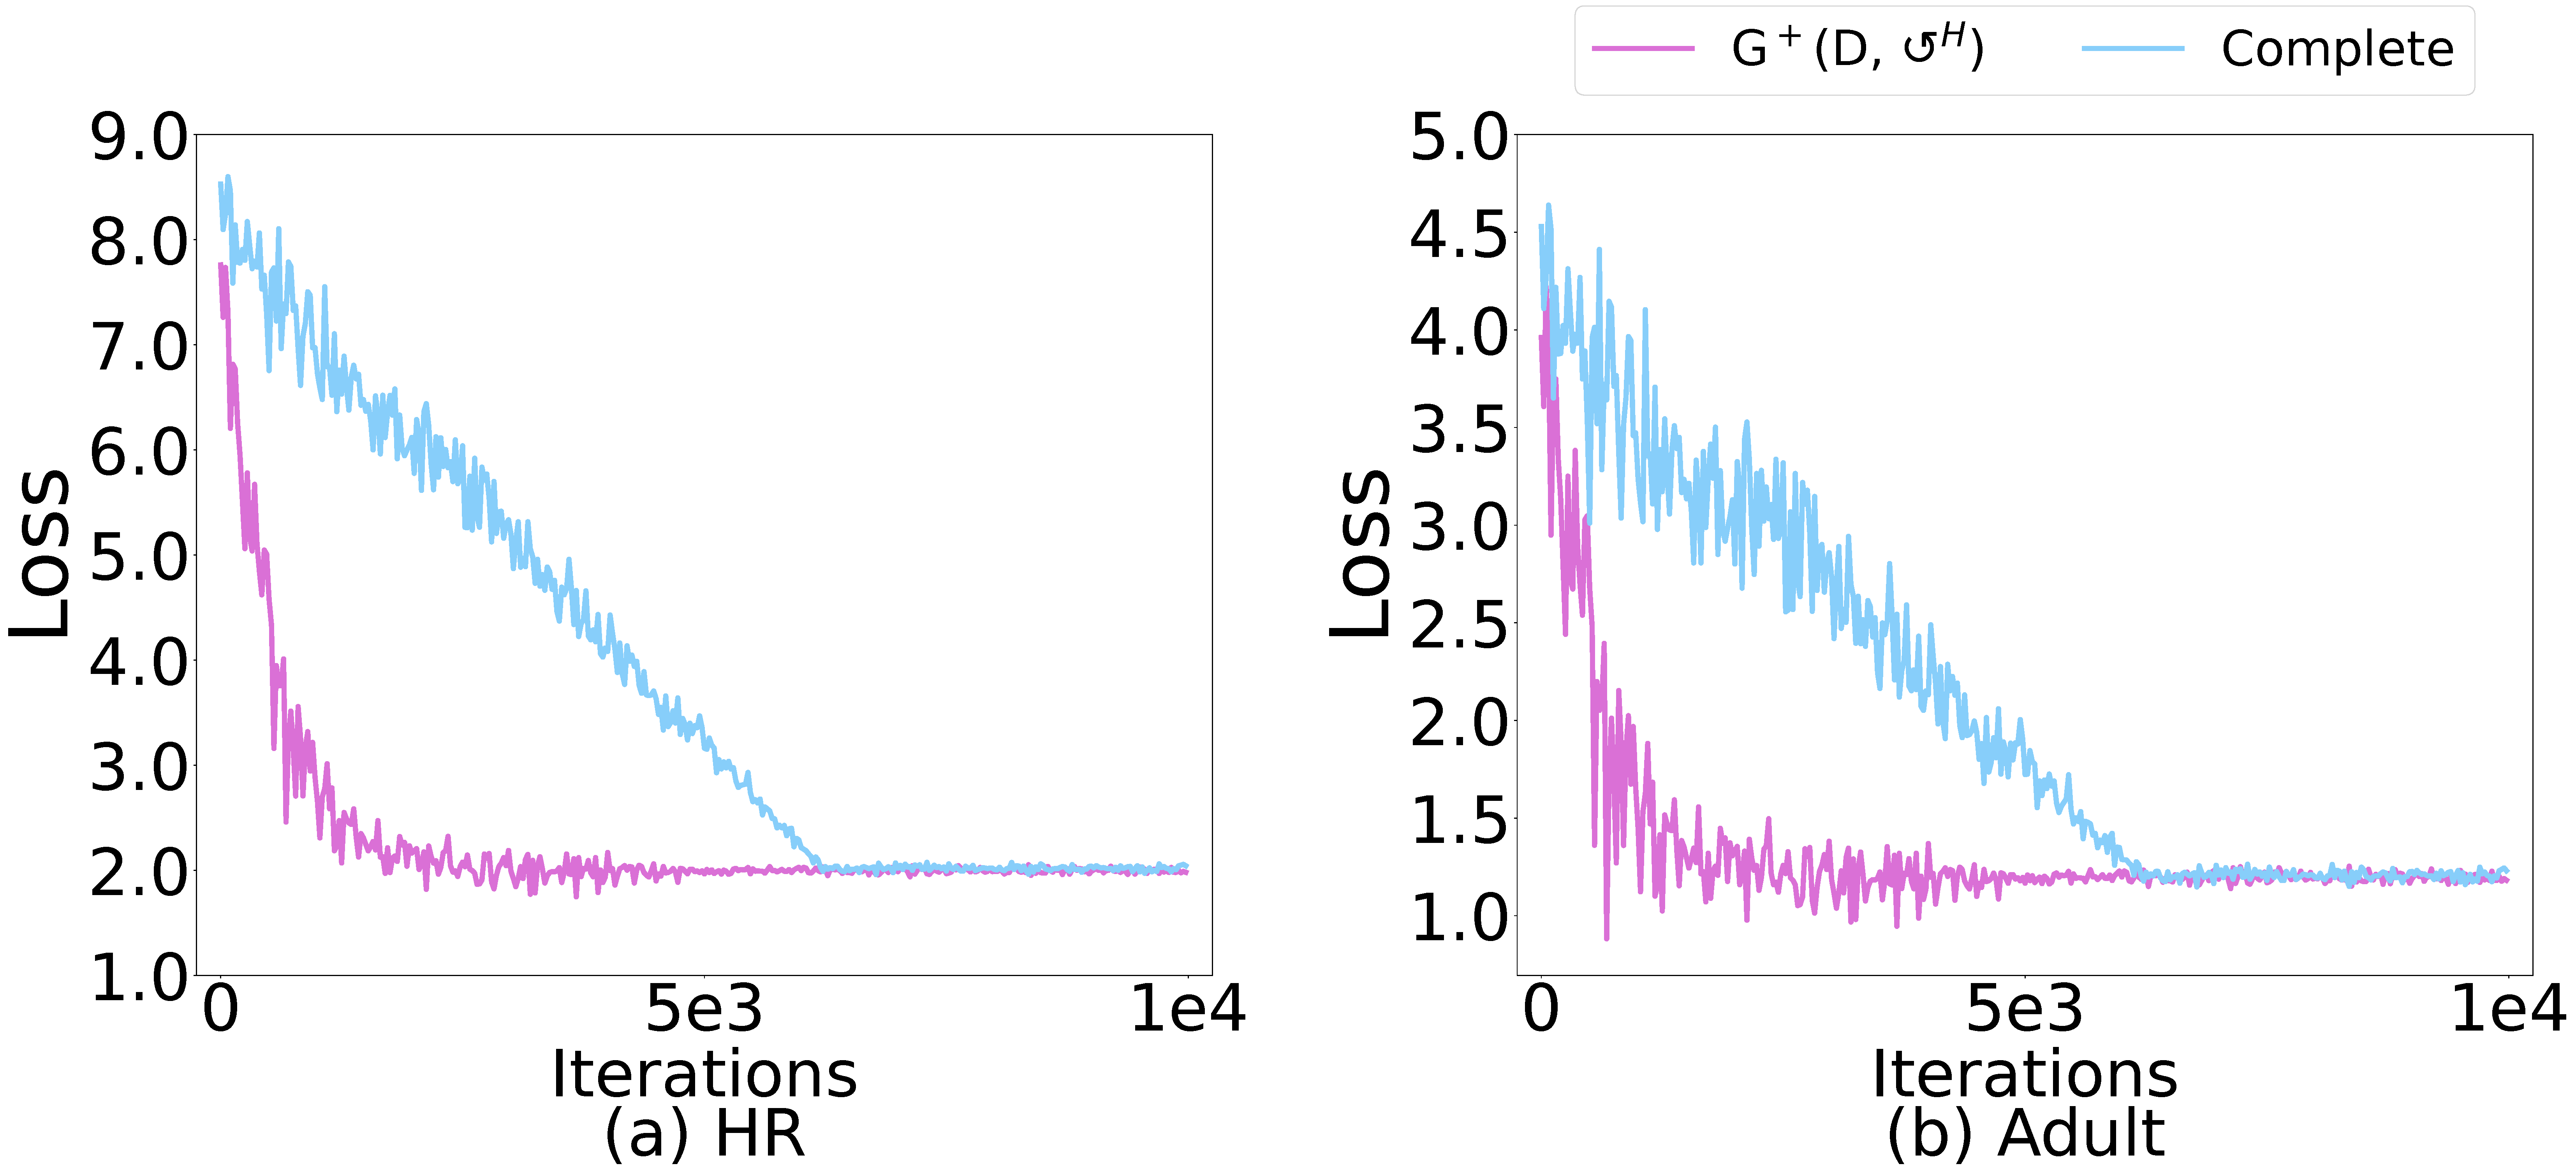
\includegraphics[width=\columnwidth]{figs/G+}
		\vspace{-1.5em}
		\caption{Loss of \texttt{GoodCore}$^+$.}
		\label{fig:real_loss_G+}
	\end{minipage}
	\vspace*{-1em}   
\end{figure}

In Section~\ref{sec:proof}, we have shown  the convergence rate of \ours theoretically. In this part, we test the convergence of training over the coreset ($\seven$) and entire data (\truth) empirically.  Figure~\ref{fig:converge_G} shows the test accuracy of two methods with the number of training iterations increasing. We can observe that on both datasets, training on the coreset converges much faster than training on the full data. 

For example, on dataset \adult, it takes $\sim$40 iterations for \ours to converge, which is  $180\times$ faster than {\truth}. This is because \ours has the same convergence rate with training over the entire dataset as discussed in the theoretical result of Section~\ref{sec:proof}, but the entire dataset (\eg  ~\adult) is $200\times$ (similar to $180\times$) larger than the coreset ($\rho=0.005$).
 That is, \ours converges with the same number of epochs  as training on the entire dataset. Since the size of coreset is much smaller, \ours is more efficient. Also, we can achieve competitive accuracy as training on full data by approximating the full gradient with a theoretical bound. 

Furthermore, we report the loss change to reflect the relation between  actual convergence rate and theoretical results. In Figure~\ref{fig:real_loss_G}, on dataset \hr, the initial loss is 8.4. According to the theoretical convergence rate $O(\frac{1}{\sqrt{k}})$ (this $k$ denotes the $k$-th epoch),  the loss should decrease to around 3.8 at the end of 5-th epoch ($\approx$ 3200-th iteration). Actually,  the  actual loss decreases to 3.25 at that time, which is close to the theoretical value.

We also test the convergence of \texttt{GoodCore}$^+$, as shown in Figure~\ref{fig:converge_G+} and 	\ref{fig:real_loss_G+}. The results  validate that the group-based method can also converge fast.

%\jks{We theoretically established the convergence rate of \ours$^+$. Then we empirically evaluate the convergence of training on the coreset ($\nine$) and the entire dataset (\truth) in Section~\ref{subsec:pq}. Figure~\ref{fig:converge_G+} depicts the test accuracy of both methods as the number of training iterations increases. It is evident that training on the coreset achieves faster convergence compared to training on the full dataset, observed across both datasets.
%For example, on dataset \adult, it takes $\sim$40 iterations for \ours$^+$ to converge, which is  $180\times$ faster than {\truth} and the same as $\seven$. This is because \ours$^+$ and \ours have the same convergence rate with training over the entire dataset, which are both $200\times$ (similar to $180\times$) smaller than the entire dataset. Consequently, \texttt{GoodCore}$^+$ converges within an equivalent number of epochs compared to training on the entire dataset. Given the substantially smaller size of the coreset, \ours$^+$ exhibits superior efficiency. Moreover, by approximating the full gradient using a theoretical bound, we can attain competitive accuracy akin to training on the complete dataset. }
 

%\jks{Alternatively, we also report the variations in loss to demonstrate the connection between the actual convergence speed and the theoretical results. As shown in Figure~\ref{fig:real_loss_G+}, on dataset \hr, the initial loss is 7.7. And the loss should decrease to around 3.5 at the end of 5-th epoch ($\approx$ 3200-th iteration) based on the theoretical convergence rate. Actually, the actual loss decreases to 3.04 at that time, which is close to the theoretical value.}

\begin{figure}[t]   
	\centering
	\begin{minipage}[t]{0.49\textwidth}
		\centering
		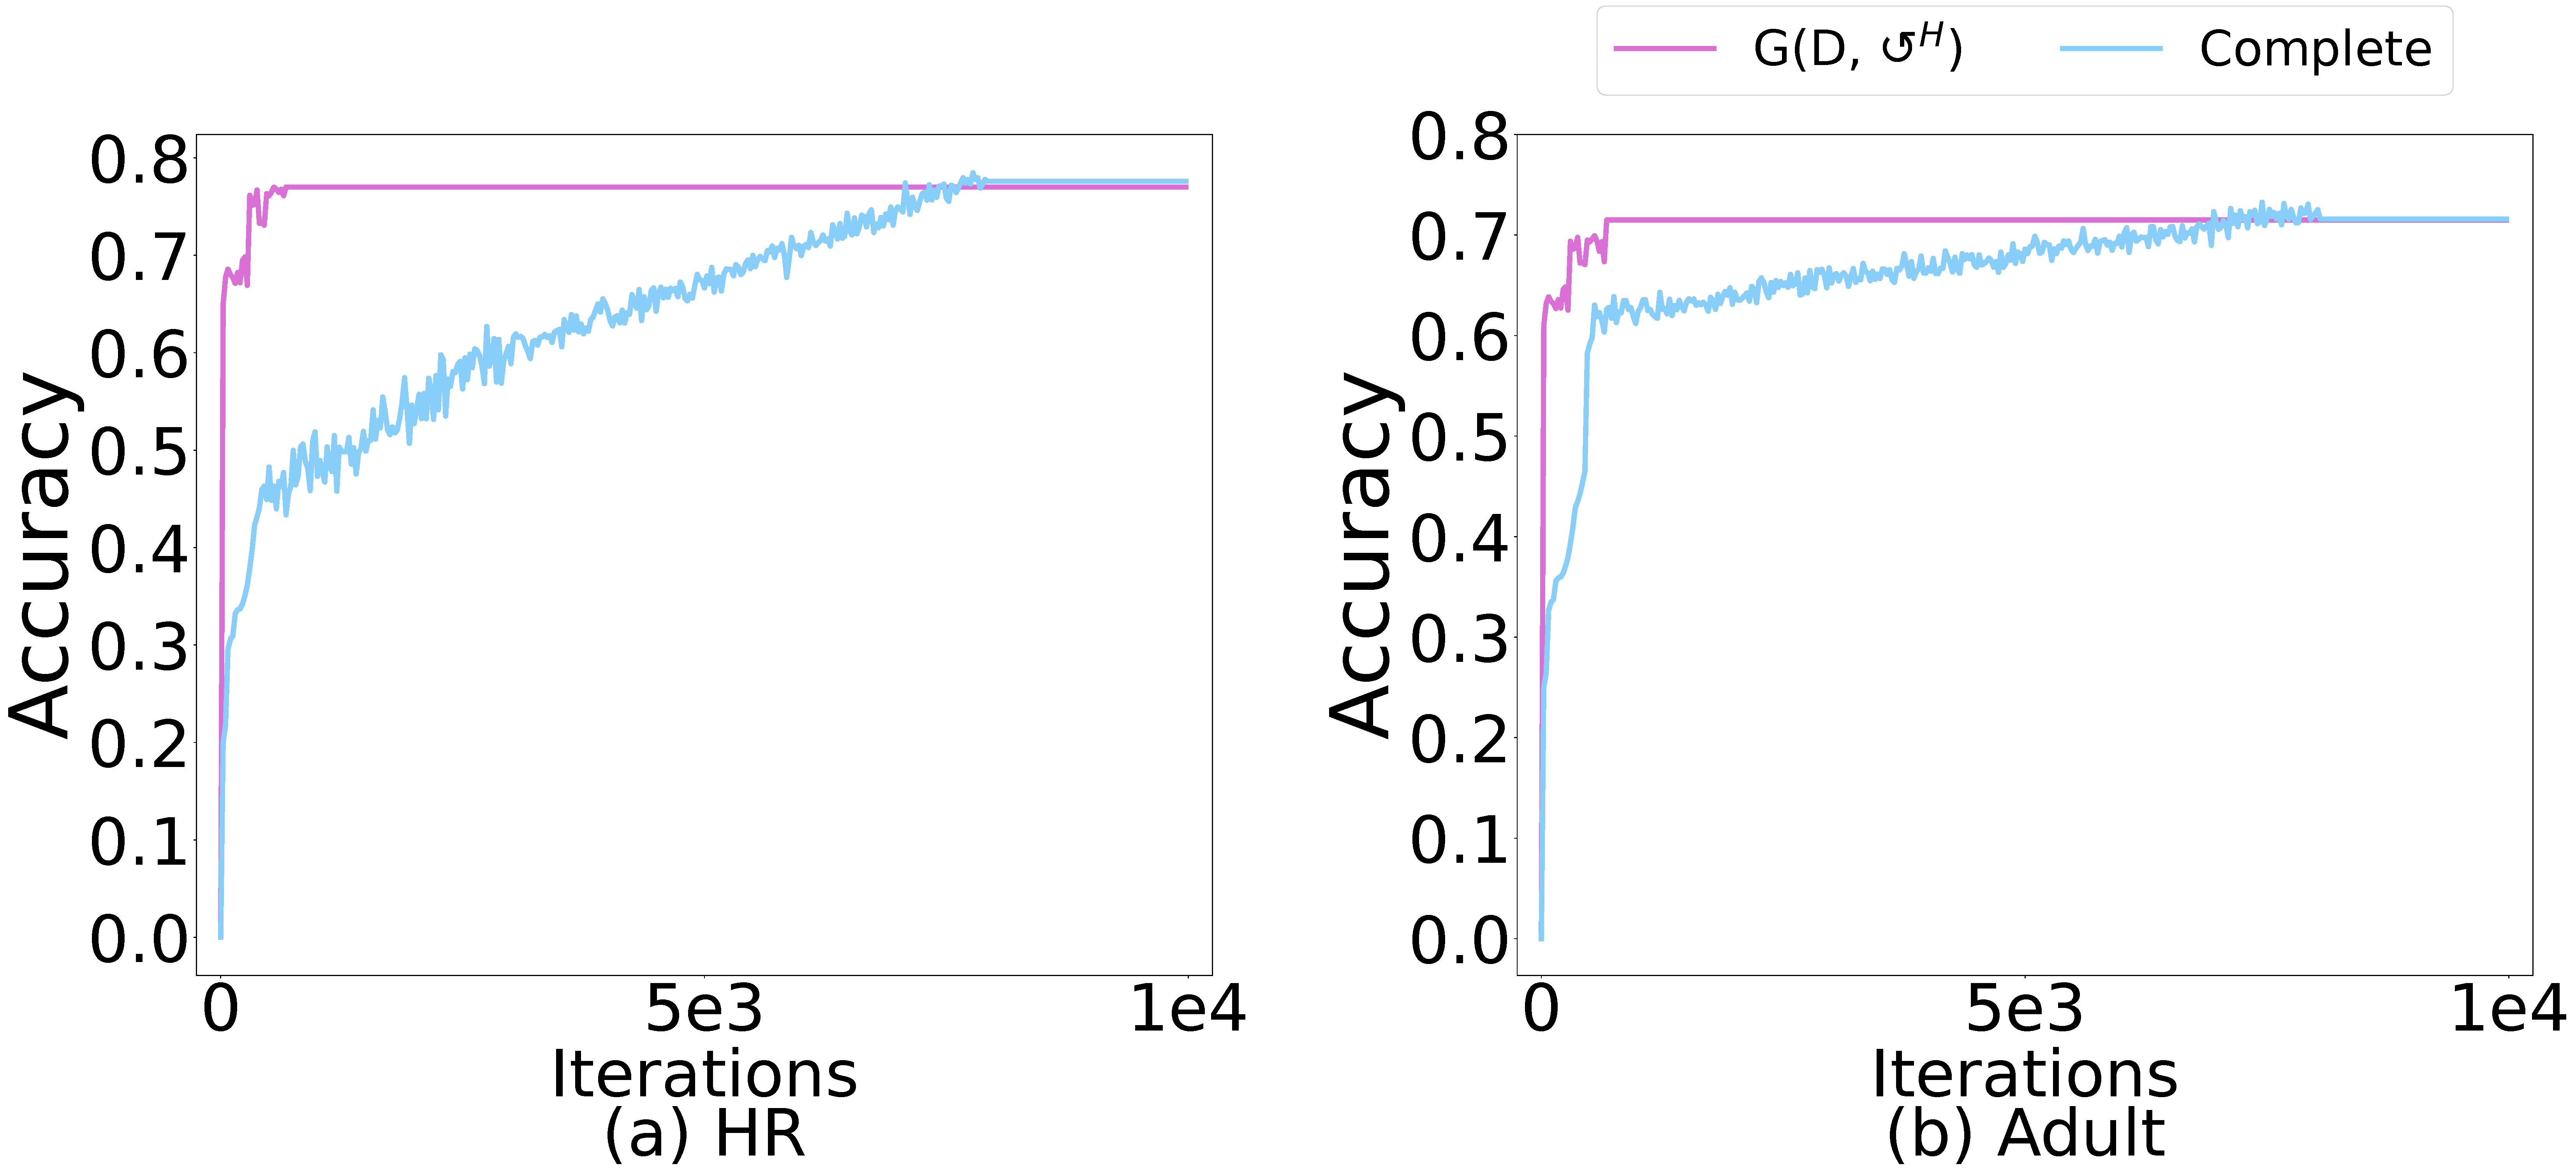
\includegraphics[width=\columnwidth]{figs/G_a}
	%	\vspace{-1.5em}
		\caption{Convergence of \ours.}
		\label{fig:converge_G}
	\end{minipage}
	\begin{minipage}[t]{0.49\textwidth}
		\centering
		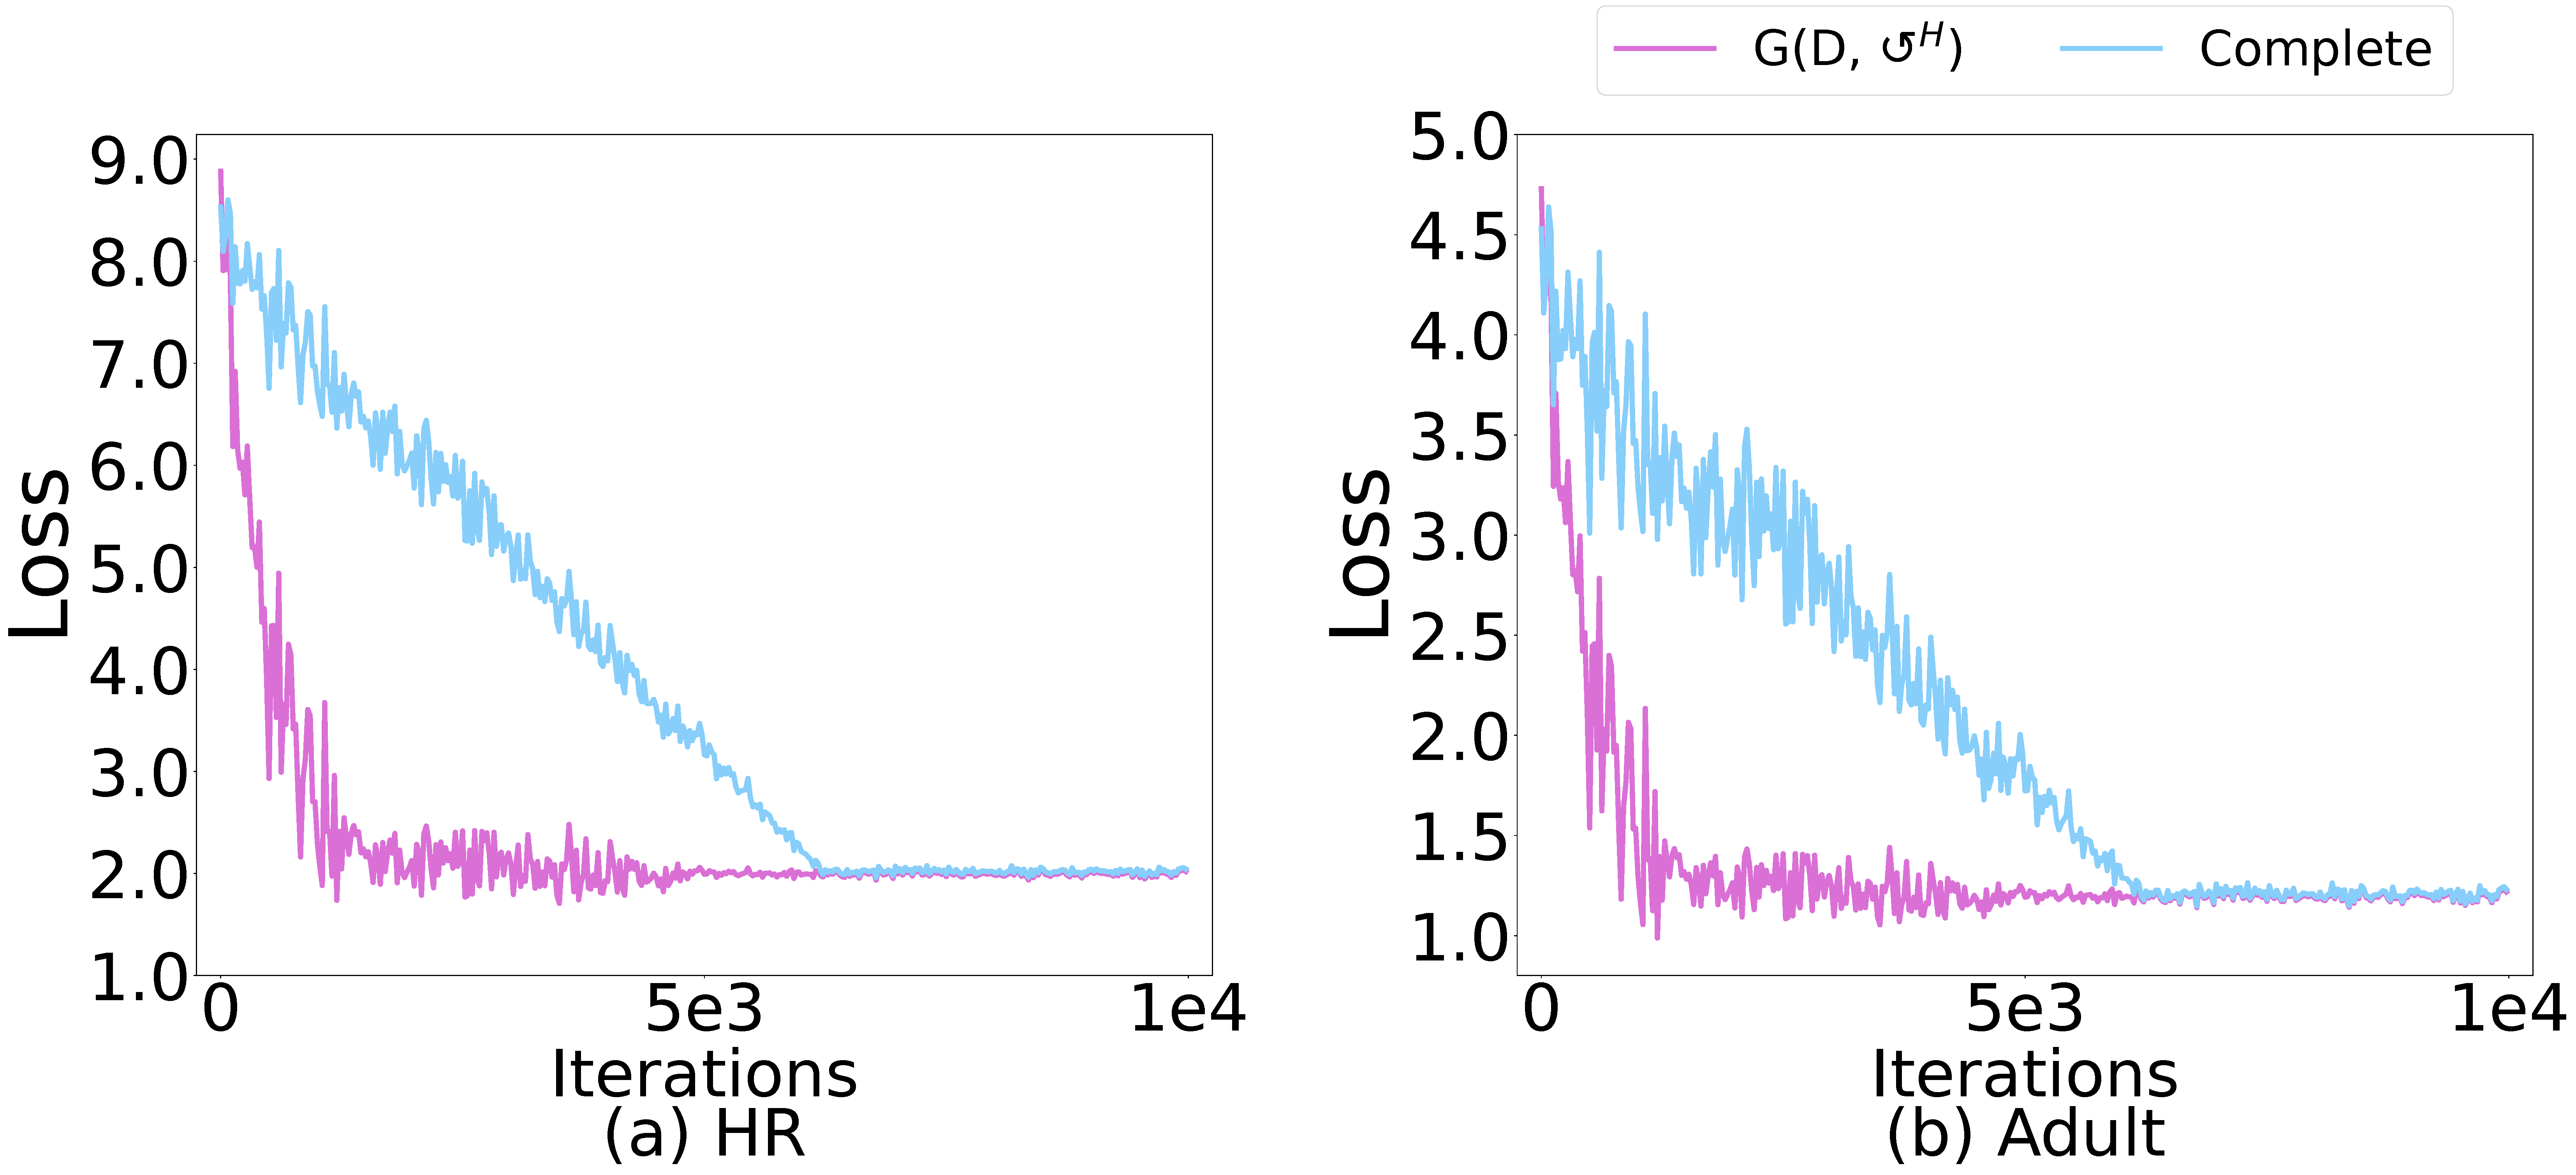
\includegraphics[width=\columnwidth]{figs/G}
	%	\vspace{-1.5em}
		\caption{Loss of \ours.}
		\label{fig:real_loss_G}
	\end{minipage}
	\vspace*{-1em}   
\end{figure}

\begin{figure}[t]   
	\centering
	\begin{minipage}[t]{0.49\textwidth}
		\centering
		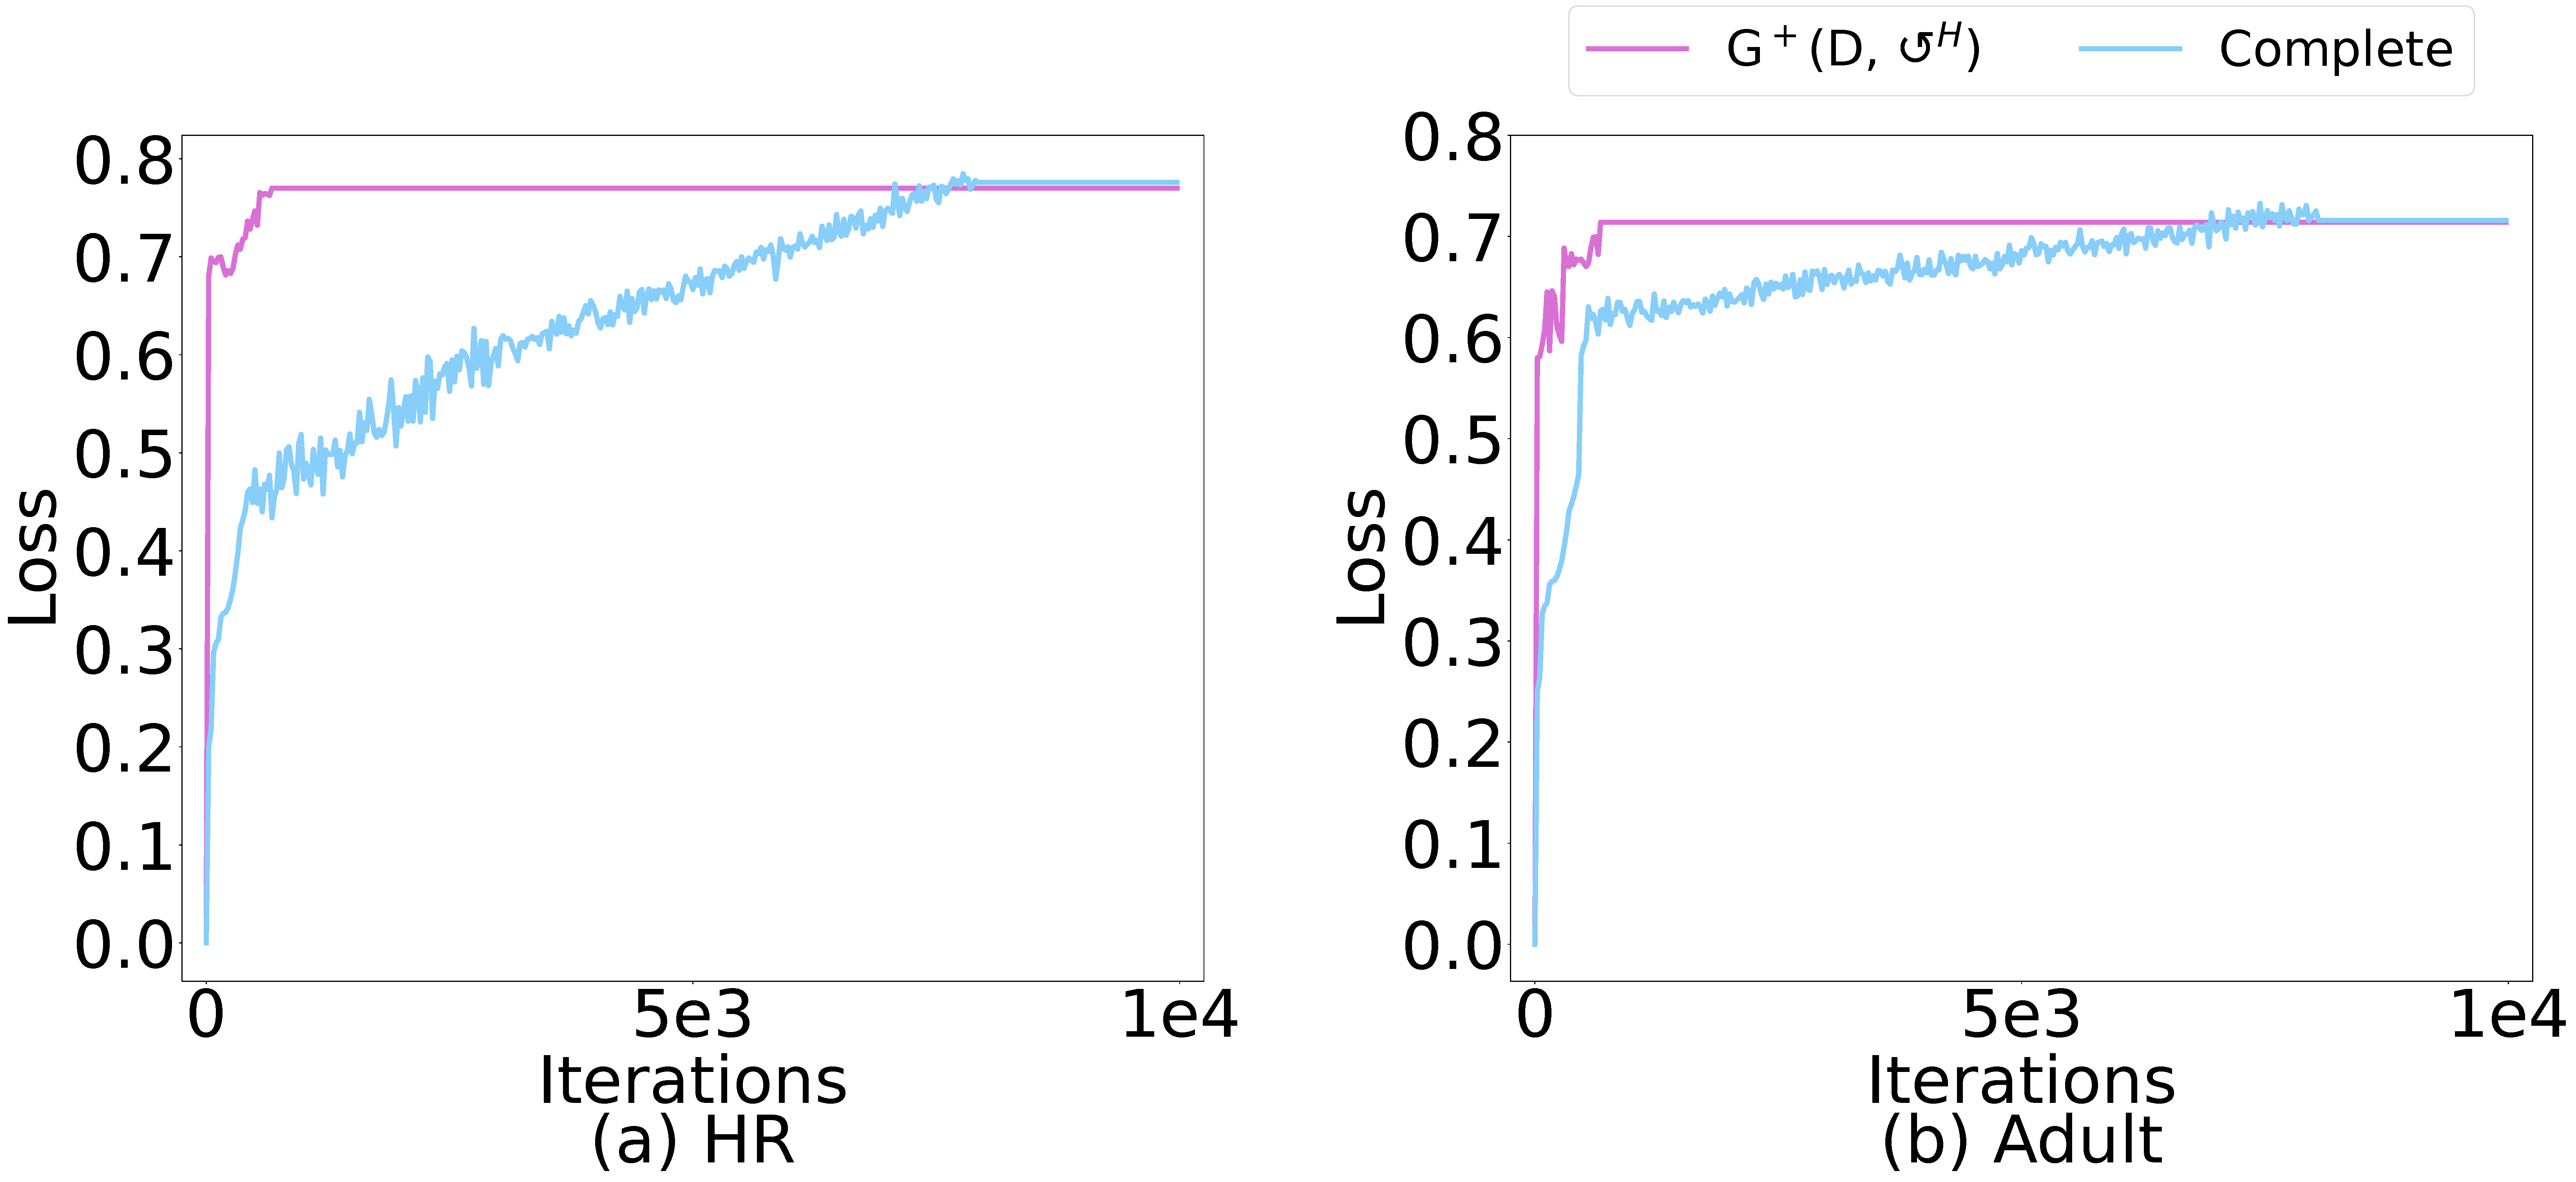
\includegraphics[width=\columnwidth]{figs/G+_a}
	%	\vspace{-1.5em}
		\caption{Convergence of \texttt{GoodCore}$^+$.}
		\label{fig:converge_G+}
	\end{minipage}
	\begin{minipage}[t]{0.49\textwidth}
		\centering
		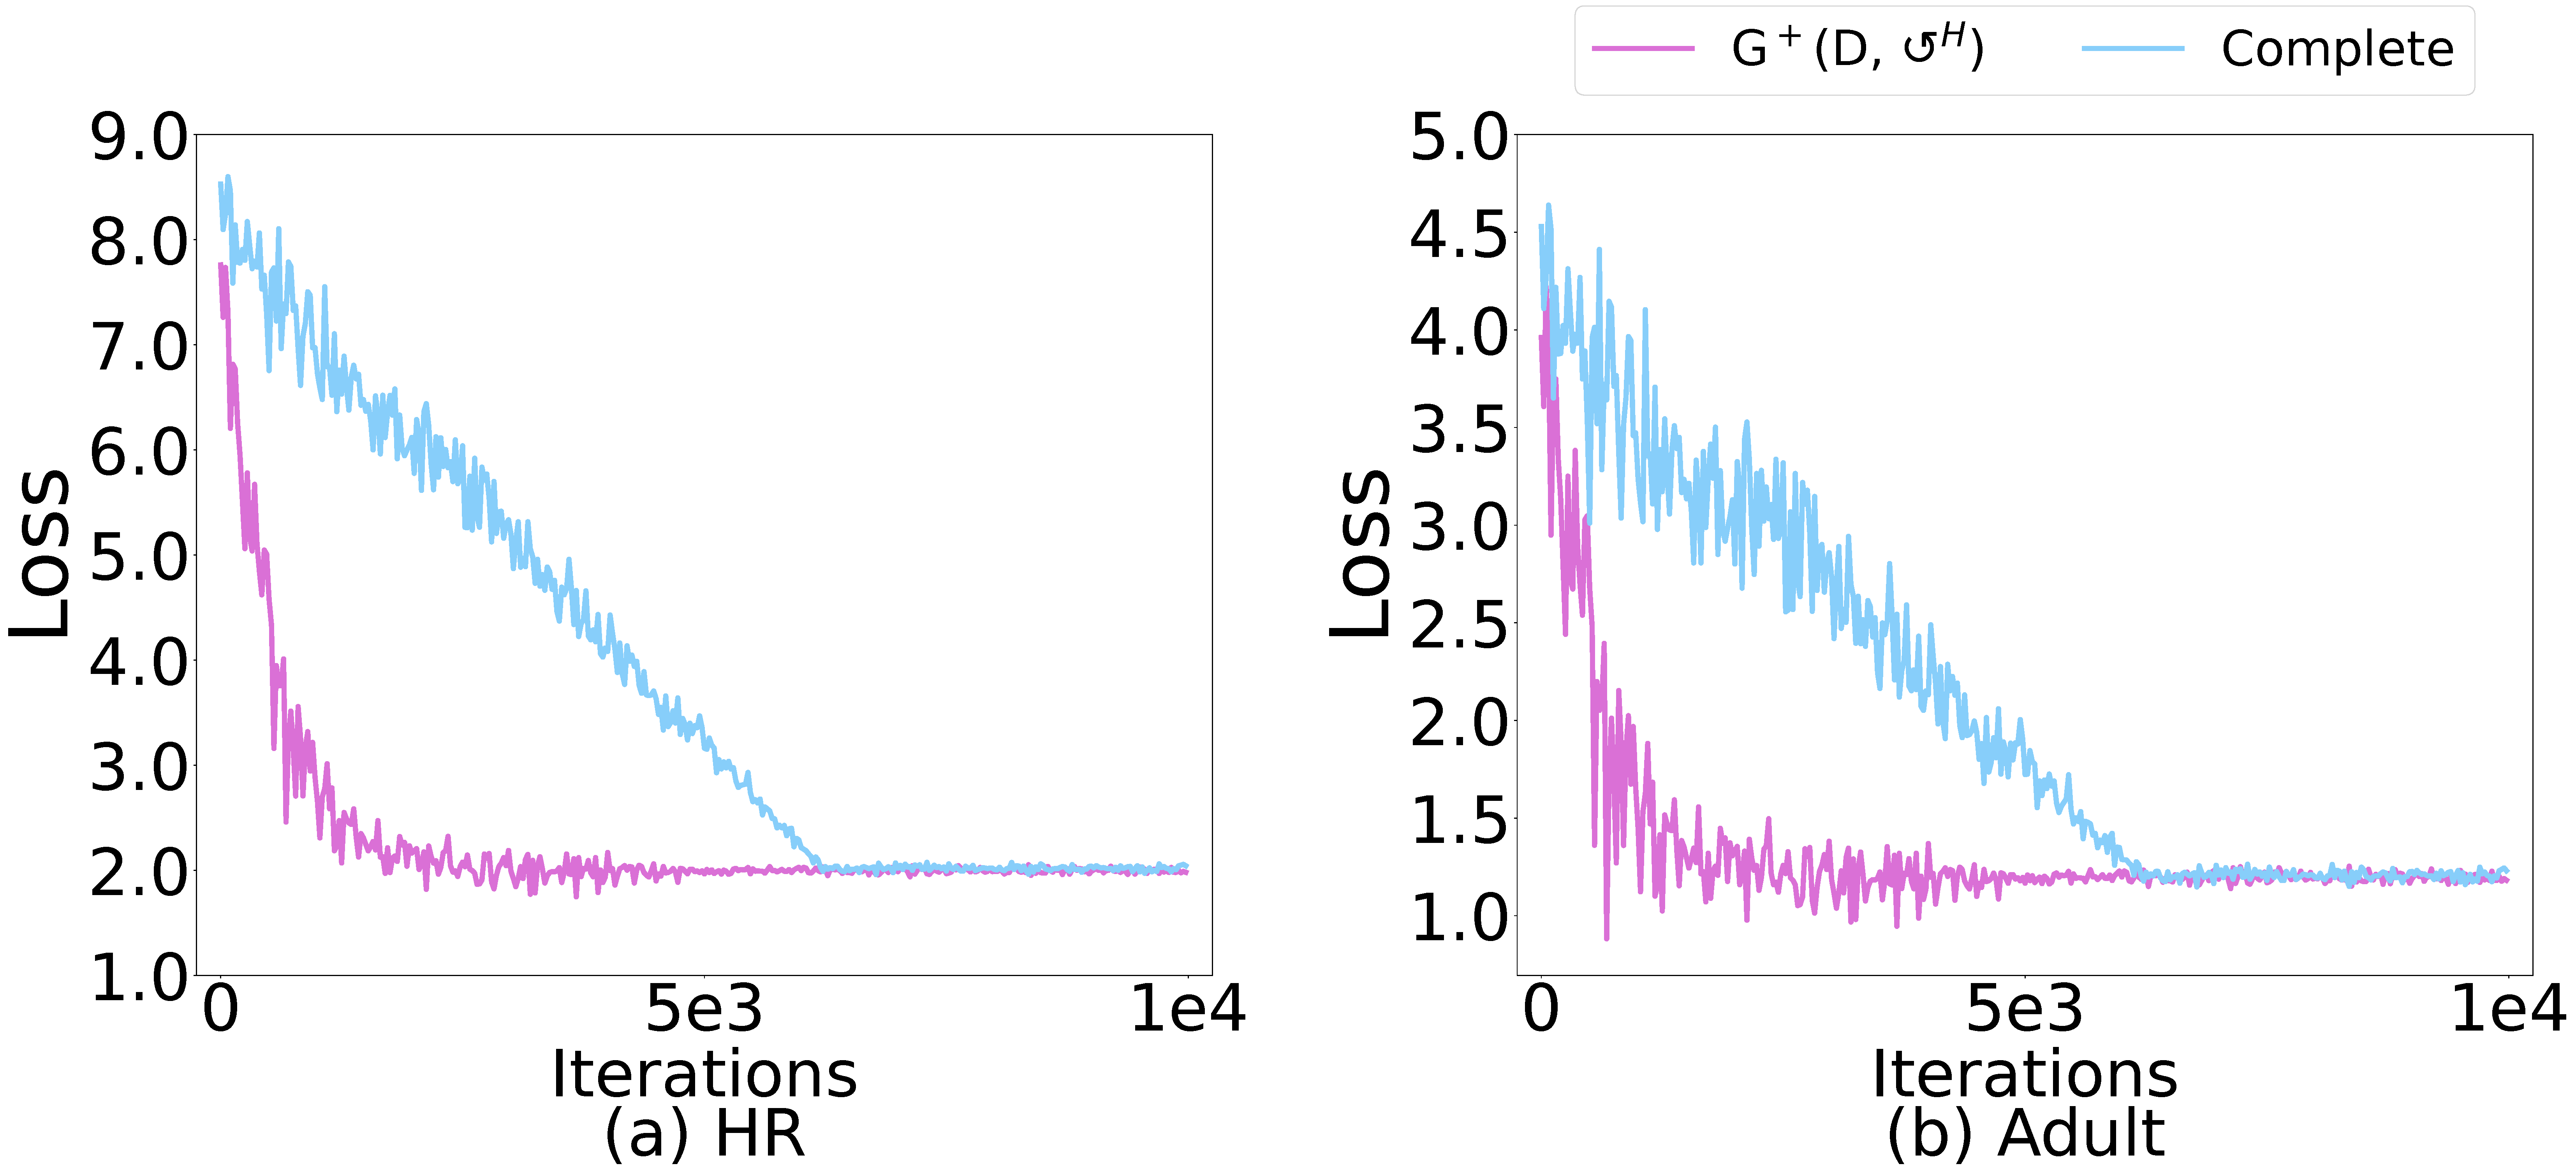
\includegraphics[width=\columnwidth]{figs/G+}
	%	\vspace{-1.5em}
		\caption{Loss of \texttt{GoodCore}$^+$.}
		\label{fig:real_loss_G+}
	\end{minipage}
	\vspace*{-1em}   
\end{figure}

%!TEX root = ../main.tex
\vspace{-0.5em}
\subsection{Sensitivity Analysis}
\label{exp:sec:sensitivity}

\noindent{\bf Varying the sample size.} In this part, we vary the sample size $h$ and evaluate the performance. The experimental results are shown in Figure~\ref{fig:samplesize}. We vary the sample size $h$ from $2^2$ to $2^{10}$. We can see that when $h$ is too small, the performance is low. The reason is that \ours cannot precisely estimate the utilities of tuples when $h$ is  small.  When the sample size increases, we can see that the performance improves rapidly and finally becomes stable, which indicates that \ours is not much sensitive to the sample size when $h$ is not too small.



\noindent{\bf Varying the downstream models.} Recap that \ours can be used on different convex models. Thus, in this part, we apply \ours on different convex models and evaluate the performance. We evaluate logistic regression and SVM for classification tasks. For regression tasks, we evaluate linear regression, ridge regression and SVM regression. We can see that  in Figure~\ref{fig:downmodel} (a) and (b), on dataset \adult, $\seven$ achieved 71.7\% accuracy for SVM, better than on logistic regression (69.4\%). Although different downstream models may have different performance, \ours can improve the model performance for the specific downstream model. In order to show that \ours can be used for other types of models like neural networks, we compare with Multilayer Perceptron (MLP, fully connected networks of 2 hidden layers with 256 nodes for each layer), although \ours does not hold
theoretical guarantee for this non-convex model. As shown in Figure~\ref{fig:downmodel}, we can see that MLP achieves almost the same performance as the ground truth. This is because the coreset selected by \ours can also represent the full dataset. However, in Figure~\ref{fig:downmodel}(c), on a large dataset \air (with metric MSE, the lower the better), neural network based methods (we also implement RNN, 2 hidden layers with 128 nodes for each layer) can have a better accuracy but the coreset cannot perfectly achieve the same performance. %Since we need to compare $\seven$ and $\eight$ with $\truth$, we drop the incomplete tuples in the original dataset and manually inject missing values. 
This may because this large dataset has more informative things to learn, and it is hard for the coreset-based solution to well represent the dataset without the theoretical guarantee.


%\add{For the MLP model, we use fully connected networks of 2 hidden layers. Each layer has 256 nodes. We find that \ours failed on \air when using non-convex model. In Figure~\ref{fig:downmodel}, we can see that MLP (2 hidden layers with 256 nodes for each layer) and RNN (2 hidden layers with 128 nodes for each layer) trained on coreset cannot achieve the same performance on the full dataset.}

%\cc{details of MLP and RNN}

\noindent{\bf Varying the percentage of incomplete tuples.} In this part, we vary the rate of missing tuples and evaluate the performance, as shown in Figure~\ref{fig:vary_misstuple_all}. 
Note that the rate  denotes the percentage of incomplete tuples rather than the cell values. Even if a tuple just has one missing attribute, it is regarded as incomplete.	
	We vary the percentage  from $20\%$ to $100\%$. We can observe that the performance does not decrease  much with the percentage increasing from $20\%$ to $50\%$, which indicates that \ours is not very sensitive to the percentage of incomplete tuples in this range. After that, the accuracy decreases because there are more missing tuples.

Besides, we also vary the rate of missing cell values in Figure~\ref{fig:realmissrate}. In this scenario, for example, 50\% missing values of a dataset  indicates more number of missing cell values than the scenario of 50\% missing tuples. Hence, we can see that the accuracy decreases more quickly than Figure~\ref{fig:vary_misstuple_all}.





\begin{figure}[t]   
	\centering
	\begin{minipage}[t]{0.38\textwidth}
		\centering
		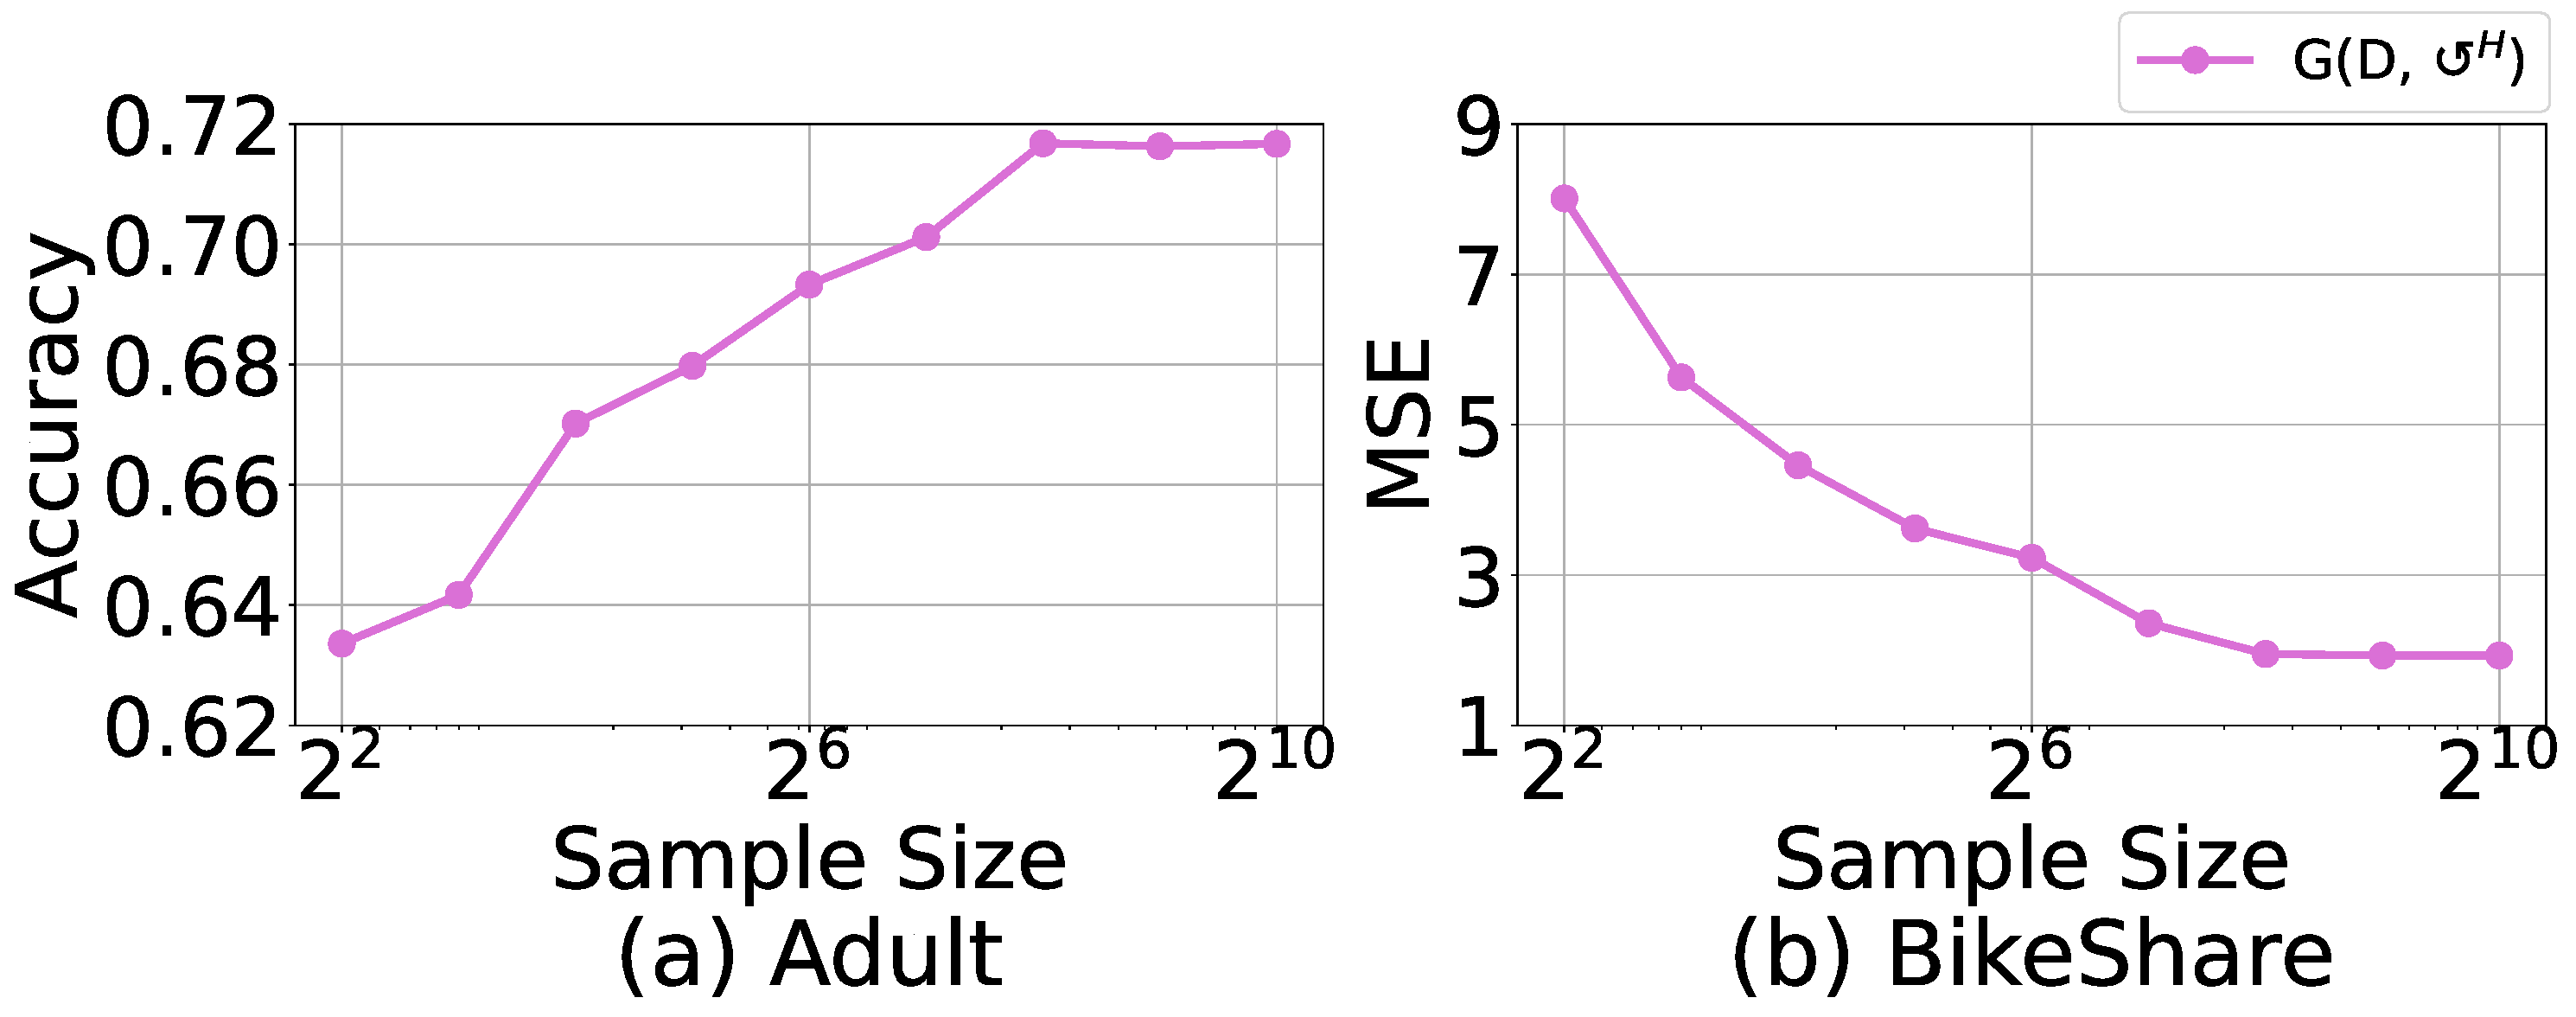
\includegraphics[width=\columnwidth]{figs/samplesize}
		\vspace{-2.5em}
		\caption{Varying sample size.}
		\label{fig:samplesize}
	\end{minipage}
	\begin{minipage}[t]{0.58\textwidth}
		\centering
		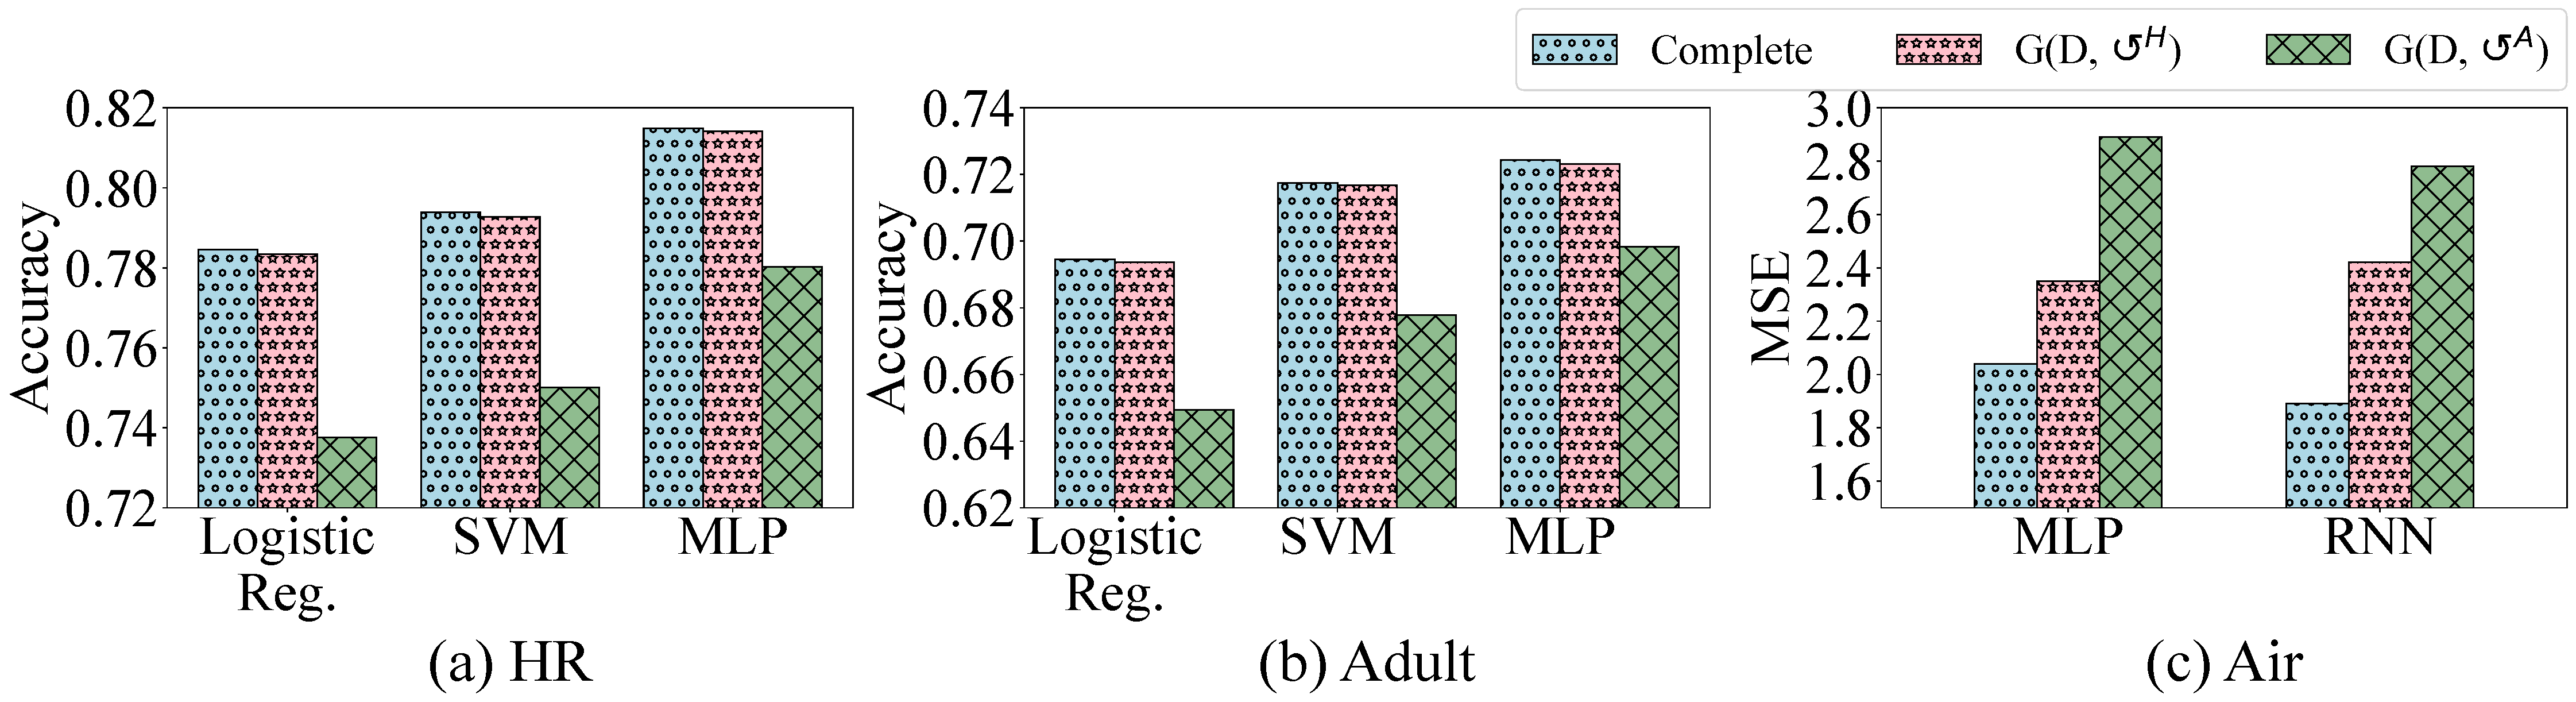
\includegraphics[width=\columnwidth]{figs/downstream_all}
		\vspace{-2.5em}
		\caption{Varying downstream model.}
		\label{fig:downmodel}
	\end{minipage}
	\vspace*{-1em}   
\end{figure}







%!TEX root = ../main.tex
%\vspace{-1em}
\section{Related Work}\label{sec:related}

\noindent{\bf Task-agnostic incomplete data imputation.}
Data imputation has been widely studied for  years. Existing  methods can be divided into two categories: statistic-based methods and learning-based methods. The former one always uses the statistic information~\cite{DBLP:journals/tsmc/FarhangfarKP07, DBLP:conf/sigmod/MayfieldNP10} (like mean, median or mode) to impute the missing values. Also, some methods compute the similarity of the incomplete tuples to the complete tuples and use the most similar one to impute the missing values~\cite{altman1992introduction, DBLP:journals/artmed/JerezMGARMF10, DBLP:conf/isese/TwalaCS05}. Recently, to improve the imputation accuracy,   many learning-based methods focus on how to use ML to learn the data distribution (\eg MissForest imputation~\cite{DBLP:journals/bioinformatics/StekhovenB12}, MICE~\cite{royston2011multiple},  IIM~\cite{DBLP:conf/icde/ZhangSSW19}), and then  use the trained model to predict the missing values. Besides traditional ML models, some deep learning models are also used for data imputation (\eg  autoencoder~\cite{DBLP:journals/corr/GondaraW17, mccoy2018variational, DBLP:journals/pr/NazabalOGV20}, GANs~\cite{DBLP:journals/nn/SpinelliSU20, DBLP:conf/icml/YoonJS18}).
 
\noindent{\bf Coreset selection.} A previous work~\cite{} has studied how to select a well-performed coreset over incomplete tuples. The extension to the previous study in this work is four-fold. First, we propose a new framework that incorporates the group-based strategy into the coreset selection process with incomplete data. Secondly, we theoretically analyze that the group-based strategy can still have a bounded GA error. Third, we propose an efficient solution to estimate the upper bound, and several strategies to reduce the number of possible worlds. Fourth, two large datasets are added and multiple experiments are conducted to demonstrate the efficacy of our proposed methods. 

%
Besides, Huang et al.~\cite{DBLP:conf/icml/HuangHLFD21} studied how to compute and continuously update the coreset while training. %, which aims  to utilize the loss of training tuples  to approximate the overall training loss of the entire training set. 
But it is rather time-consuming because of the training process. 
 To solve this problem, works~\cite{DBLP:conf/icml/CampbellB18, DBLP:journals/corr/BravermanFL16}   selected the coreset without training in advance, but they can only be customized to particular model types respectively. %The basic idea is to compute a sensitive score for each tuple, and the higher the score, the more likely the tuple should be in the coreset. 
 Another line of works~\cite{DBLP:conf/icml/MirzasoleimanBL20, DBLP:conf/nips/MirzasoleimanCL20, DBLP:conf/emnlp/KirchhoffB14} focused on selecting the coreset to approximate the full gradient without training in advance for multiple model types, which is regarded as an optimization problem that can be solved  by the three nested loops framework (see Section~\ref{subset:sigletable}).

In short, none of them considers coreset selection over incomplete data. Different from them, we make the first attempt to select coresets over incomplete data.

\noindent{\bf Data cleaning for ML.} Recently, there have  been several works that clean the data to optimize the ML model. 
In contrast to the above discussion about task-agnostic incomplete data imputation, data cleaning for ML is task-aware, which triggers new technical challenges.
SampleClean~\cite{DBLP:journals/debu/KrishnanWFGKM015} focuses on cleaning selected samples, so as to answer  SQL aggregate  queries  more efficiently, but it is not for any model.
%
 CPClean~\cite{DBLP:journals/pvldb/KarlasLWGC0020} proposes certain prediction to impute missing data for optimizing ML models. Different from us, it is customized to nearest neighbor classifiers rather than convex models solved by the gradient decent algorithm. 
  %
  BoostClean~\cite{DBLP:journals/corr/abs-1711-01299} regards data cleaning as a boosting problem that iteratively
 selects from a predefined set of cleaning algorithms, so as to continuously maximize the accuracy of  a validation set with training iteratively. 
Closer to our work is ActiveClean~\cite{DBLP:journals/pvldb/KrishnanWWFG16}, which progressively cleans the data tuples that are likely to much influence the model   measured by the gradients. 
%\cc{
Different from us,  given a budget $K$, we can select the coreset without training, but ActiveClean needs to train iteratively  and label a set of   validation  dataset.  We empirically show that our method outperforms ActiveClean on model accuracy and efficiency in Section~\ref{sec:exp}.
%}.
%(2) ActiveClean uses heuristics to measure the influence of tuples to the model gradients, which may not be accurate.
% Moreover, we  ActiveClean to the data imputation problem and compare with it in Section~\ref{sec:exp}.}

%ActiveClean iteratively estimates the impact of the dirty data and samples a batch of dirty data that have the most impact on the model. Then, ActiveClean asks human to clean the batch of dirty data. The main difference between ActiveClean and \ours is ActiveClean needs to iteratively train the model, since it relies on the feedback from both human and model to estimate the impact of the dirty data.


\noindent{\bf Data Preparation for AI.}
Data preparation~\cite{chai2020crowdchart} can be utilized to improve the effectiveness of ML model, including data discovery~\cite{liu2021automatic, chai2022selective, liu2022feature},  data cleaning~\cite{hao2020outdated,chai2020human}, data labeling~\cite{chai2016cost, chai2018partial, li2018cdb}, data cleaning~\cite{miao2022experimental, gao2018query,miao2018incomplete, miao2021efficient,wu2022interactive,ge2020hybrid} and data exploration~\cite{qin2020interactively,qin2021ranking}.
%!TEX root = ../main.tex
%\vspace{-1em}
\section{Conclusion}

In this paper, we propose the \ours framework to select a good coreset over the incomplete data, which achieves data-effective and data-efficient ML. We formulate it as an expected optimal coreset selection problem, which is NP-hard. Then we propose a greedy algorithm with an approximation ratio. We also propose to involve imputation-in-the-loop strategies into \ours to further improve the efficiency. We conduct experiments on real-world datasets to verify the effectiveness and efficiency of \ours.

	
%\balance
\clearpage

%\bibliographystyle{abbrv}
\normalem
\bibliographystyle{ACM-Reference-Format}
\bibliography{DA}

\end{document}
\endinput
%%
%% End of file `sample-acmsmall.tex'.
